% Options for packages loaded elsewhere
\PassOptionsToPackage{unicode}{hyperref}
\PassOptionsToPackage{hyphens}{url}
%
\documentclass[
]{book}
\usepackage{lmodern}
\usepackage{amssymb,amsmath}
\usepackage{ifxetex,ifluatex}
\ifnum 0\ifxetex 1\fi\ifluatex 1\fi=0 % if pdftex
  \usepackage[T1]{fontenc}
  \usepackage[utf8]{inputenc}
  \usepackage{textcomp} % provide euro and other symbols
\else % if luatex or xetex
  \usepackage{unicode-math}
  \defaultfontfeatures{Scale=MatchLowercase}
  \defaultfontfeatures[\rmfamily]{Ligatures=TeX,Scale=1}
\fi
% Use upquote if available, for straight quotes in verbatim environments
\IfFileExists{upquote.sty}{\usepackage{upquote}}{}
\IfFileExists{microtype.sty}{% use microtype if available
  \usepackage[]{microtype}
  \UseMicrotypeSet[protrusion]{basicmath} % disable protrusion for tt fonts
}{}
\makeatletter
\@ifundefined{KOMAClassName}{% if non-KOMA class
  \IfFileExists{parskip.sty}{%
    \usepackage{parskip}
  }{% else
    \setlength{\parindent}{0pt}
    \setlength{\parskip}{6pt plus 2pt minus 1pt}}
}{% if KOMA class
  \KOMAoptions{parskip=half}}
\makeatother
\usepackage{xcolor}
\IfFileExists{xurl.sty}{\usepackage{xurl}}{} % add URL line breaks if available
\IfFileExists{bookmark.sty}{\usepackage{bookmark}}{\usepackage{hyperref}}
\hypersetup{
  pdftitle={Introduction aux Data Sciences},
  pdfauthor={Christophe Benavent - Université Paris Dauphine},
  hidelinks,
  pdfcreator={LaTeX via pandoc}}
\urlstyle{same} % disable monospaced font for URLs
\usepackage{color}
\usepackage{fancyvrb}
\newcommand{\VerbBar}{|}
\newcommand{\VERB}{\Verb[commandchars=\\\{\}]}
\DefineVerbatimEnvironment{Highlighting}{Verbatim}{commandchars=\\\{\}}
% Add ',fontsize=\small' for more characters per line
\usepackage{framed}
\definecolor{shadecolor}{RGB}{248,248,248}
\newenvironment{Shaded}{\begin{snugshade}}{\end{snugshade}}
\newcommand{\AlertTok}[1]{\textcolor[rgb]{0.94,0.16,0.16}{#1}}
\newcommand{\AnnotationTok}[1]{\textcolor[rgb]{0.56,0.35,0.01}{\textbf{\textit{#1}}}}
\newcommand{\AttributeTok}[1]{\textcolor[rgb]{0.77,0.63,0.00}{#1}}
\newcommand{\BaseNTok}[1]{\textcolor[rgb]{0.00,0.00,0.81}{#1}}
\newcommand{\BuiltInTok}[1]{#1}
\newcommand{\CharTok}[1]{\textcolor[rgb]{0.31,0.60,0.02}{#1}}
\newcommand{\CommentTok}[1]{\textcolor[rgb]{0.56,0.35,0.01}{\textit{#1}}}
\newcommand{\CommentVarTok}[1]{\textcolor[rgb]{0.56,0.35,0.01}{\textbf{\textit{#1}}}}
\newcommand{\ConstantTok}[1]{\textcolor[rgb]{0.00,0.00,0.00}{#1}}
\newcommand{\ControlFlowTok}[1]{\textcolor[rgb]{0.13,0.29,0.53}{\textbf{#1}}}
\newcommand{\DataTypeTok}[1]{\textcolor[rgb]{0.13,0.29,0.53}{#1}}
\newcommand{\DecValTok}[1]{\textcolor[rgb]{0.00,0.00,0.81}{#1}}
\newcommand{\DocumentationTok}[1]{\textcolor[rgb]{0.56,0.35,0.01}{\textbf{\textit{#1}}}}
\newcommand{\ErrorTok}[1]{\textcolor[rgb]{0.64,0.00,0.00}{\textbf{#1}}}
\newcommand{\ExtensionTok}[1]{#1}
\newcommand{\FloatTok}[1]{\textcolor[rgb]{0.00,0.00,0.81}{#1}}
\newcommand{\FunctionTok}[1]{\textcolor[rgb]{0.00,0.00,0.00}{#1}}
\newcommand{\ImportTok}[1]{#1}
\newcommand{\InformationTok}[1]{\textcolor[rgb]{0.56,0.35,0.01}{\textbf{\textit{#1}}}}
\newcommand{\KeywordTok}[1]{\textcolor[rgb]{0.13,0.29,0.53}{\textbf{#1}}}
\newcommand{\NormalTok}[1]{#1}
\newcommand{\OperatorTok}[1]{\textcolor[rgb]{0.81,0.36,0.00}{\textbf{#1}}}
\newcommand{\OtherTok}[1]{\textcolor[rgb]{0.56,0.35,0.01}{#1}}
\newcommand{\PreprocessorTok}[1]{\textcolor[rgb]{0.56,0.35,0.01}{\textit{#1}}}
\newcommand{\RegionMarkerTok}[1]{#1}
\newcommand{\SpecialCharTok}[1]{\textcolor[rgb]{0.00,0.00,0.00}{#1}}
\newcommand{\SpecialStringTok}[1]{\textcolor[rgb]{0.31,0.60,0.02}{#1}}
\newcommand{\StringTok}[1]{\textcolor[rgb]{0.31,0.60,0.02}{#1}}
\newcommand{\VariableTok}[1]{\textcolor[rgb]{0.00,0.00,0.00}{#1}}
\newcommand{\VerbatimStringTok}[1]{\textcolor[rgb]{0.31,0.60,0.02}{#1}}
\newcommand{\WarningTok}[1]{\textcolor[rgb]{0.56,0.35,0.01}{\textbf{\textit{#1}}}}
\usepackage{longtable,booktabs}
% Correct order of tables after \paragraph or \subparagraph
\usepackage{etoolbox}
\makeatletter
\patchcmd\longtable{\par}{\if@noskipsec\mbox{}\fi\par}{}{}
\makeatother
% Allow footnotes in longtable head/foot
\IfFileExists{footnotehyper.sty}{\usepackage{footnotehyper}}{\usepackage{footnote}}
\makesavenoteenv{longtable}
\usepackage{graphicx,grffile}
\makeatletter
\def\maxwidth{\ifdim\Gin@nat@width>\linewidth\linewidth\else\Gin@nat@width\fi}
\def\maxheight{\ifdim\Gin@nat@height>\textheight\textheight\else\Gin@nat@height\fi}
\makeatother
% Scale images if necessary, so that they will not overflow the page
% margins by default, and it is still possible to overwrite the defaults
% using explicit options in \includegraphics[width, height, ...]{}
\setkeys{Gin}{width=\maxwidth,height=\maxheight,keepaspectratio}
% Set default figure placement to htbp
\makeatletter
\def\fps@figure{htbp}
\makeatother
\setlength{\emergencystretch}{3em} % prevent overfull lines
\providecommand{\tightlist}{%
  \setlength{\itemsep}{0pt}\setlength{\parskip}{0pt}}
\setcounter{secnumdepth}{5}
\usepackage{booktabs}
\usepackage{amsthm}
\makeatletter
\def\thm@space@setup{%
  \thm@preskip=8pt plus 2pt minus 4pt
  \thm@postskip=\thm@preskip
}
\makeatother
\usepackage[]{natbib}
\bibliographystyle{apalike}

\title{Introduction aux Data Sciences}
\author{Christophe Benavent - Université Paris Dauphine}
\date{2022-03-27}

\begin{document}
\maketitle

{
\setcounter{tocdepth}{1}
\tableofcontents
}
\hypertarget{pruxe9face}{%
\chapter{Préface}\label{pruxe9face}}

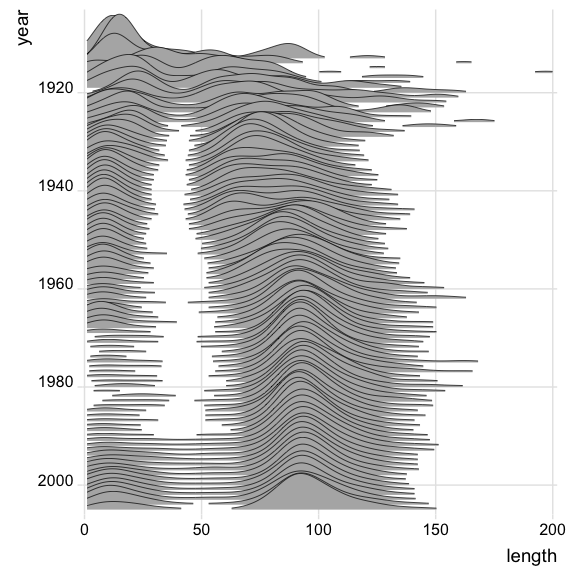
\includegraphics{./Images/ggridge.png}

Ce bookdown reprend les éléments d'un cours de data science avec r. Il a pour but d'être reproductible, c'est pourquoi le choix de ce support et des jeux de données associés. Il sera dynamique, modifié à mesure de nos cours, séminaires et ateliers.

L'illustration représente l'évolution de la longueur des films de la base Imbd et raconte en chiffres une part de l'histoire du cinema. Jusqu'au années la longueur est hétérogène mais au tournant des années 30, la distribution se stabilise, les court-métragessont de l'ordre de 15mn, et voient leurs durée se raccourcir avec les décénnies, le genre menace de disparaitredans les années 80 et reprend du poil de la bête dans les années 2000. Les films longs voient leur longueur s'accroitre et se stabiliser autur de un peu moins de 100 mn, soit une heure et trente minutes. On observera enfin qu'au cours des années 1990 les film de taille intermédiaires réapparaissent.

Dans ce graphique il y a tous les éléments des data sciences modernes : un jeu de donnée riche et systématique, un modèle statistique fondamentale avec la notion de densité de probabilité, une mesure, un critère de comparaison. Les diagrammes ridges sont inspirée de la pochette de l'album \href{https://www.youtube.com/watch?v=7PtvIr2oiaE}{Unknown Pleasures de Joy division} sorti en pleine New Wave , en 1979. Un article de Vice en rappele l'\href{https://i-d.vice.com/fr/article/pabjam/pourquoi-cette-pochette-dalbum-de-joy-division-a-inspire-le-monde-entier}{origine et le destin de ce graphisme}

\hypertarget{plan-du-manuel}{%
\section{Plan du manuel}\label{plan-du-manuel}}

Les chapitres projetés

\begin{itemize}
\tightlist
\item
  1 - L'environnement r
\item
  2 - Installation et prise en main
\item
  3 - Usage de ggplot - uni et bivarié
\item
  4 - Usage de ggplot - multivarié
\item
  6 - Analyse de variance et régression linéraire
\item
  5 - Tables
\item
  6 - Modèles factoriels ( Psych)
\item
  7 - AFC
\item
  8 - MDS
\item
  9 - Clustering
\item
  10 - Analyse de réseaux
\item
  10 - Modèle d'équations structurelles (Lavaan)
\item
  11 - Modèle linéaire généralisé
\item
  12 - Modèles à décomposition d'erreur
\item
  13 - Times series
\item
  14 - Analyse geospatiale
\item
  15 - Machine learning
\end{itemize}

\hypertarget{les-jeux-de-donnuxe9es}{%
\section{Les jeux de données}\label{les-jeux-de-donnuxe9es}}

Au cours du développement, plusieurs cas pratiques - souvent réduit en volume pour rester exemplaire, seront employés. Les donées seront partagées.

En voici la présentation systématique.

disponibles dans le \href{https://benaventc.github.io//}{repositery} avec le code du book. Les amendements et améliorations sont souhaitées et attendues.

\hypertarget{le-cadre-technique-et-les-packages-utilisuxe9s}{%
\section{Le cadre technique et les packages utilisés}\label{le-cadre-technique-et-les-packages-utilisuxe9s}}

Ce \emph{livre} est écrit en \textbf{Markdown} \citep{allaire_rmarkdown_2021} et avec le package \textbf{Bookdown} \citep{R-bookdown}

Le code s'appuie très largement sur \textbf{tidyverse} et emploie largement les ressources de \textbf{ggplot} . Les packages seront introduits au fur et à mesure. En voici la liste complète.

\begin{Shaded}
\begin{Highlighting}[]
\KeywordTok{options}\NormalTok{(}\DataTypeTok{tinytex.verbose =} \OtherTok{TRUE}\NormalTok{)}

\NormalTok{knitr}\OperatorTok{::}\NormalTok{opts_chunk}\OperatorTok{$}\KeywordTok{set}\NormalTok{(}\DataTypeTok{echo =} \OtherTok{TRUE}\NormalTok{, }\DataTypeTok{include=}\OtherTok{TRUE}\NormalTok{, }\DataTypeTok{cache=}\OtherTok{TRUE}\NormalTok{, }\DataTypeTok{message=}\OtherTok{FALSE}\NormalTok{, }\DataTypeTok{warning=}\OtherTok{FALSE}\NormalTok{)}

\CommentTok{#boite à outils et dataviz}
\KeywordTok{library}\NormalTok{(tidyverse) }\CommentTok{# inclut ggplot pour la viz, readr et }
\KeywordTok{library}\NormalTok{(cowplot) }\CommentTok{#pour créer des graphiques composés}
\KeywordTok{library}\NormalTok{(ggridges) }\CommentTok{# le joy division touch}
\KeywordTok{library}\NormalTok{(ggmosaic)}

\CommentTok{#networks}
\KeywordTok{library}\NormalTok{(igraph)}
\KeywordTok{library}\NormalTok{(ggraph)}

\CommentTok{# Accéder aux données}
\KeywordTok{library}\NormalTok{(rtweet)  }\CommentTok{# une interface efficace pour interroger l'api de Twitter}

\CommentTok{# NLP}
\KeywordTok{library}\NormalTok{(tokenizers)}
\KeywordTok{library}\NormalTok{(quanteda)}
\KeywordTok{library}\NormalTok{(quanteda.textstats)}
\KeywordTok{library}\NormalTok{(udpipe) }\CommentTok{#annotation syntaxique}
\KeywordTok{library}\NormalTok{(tidytext)}
\KeywordTok{library}\NormalTok{(cleanNLP) }\CommentTok{#annotation syntaxique}

\CommentTok{#sentiment}
\KeywordTok{library}\NormalTok{(syuzhet)             }\CommentTok{#analyse du sentimeent}



\CommentTok{#mise en page des tableaux}
\KeywordTok{library}\NormalTok{(flextable)}


\CommentTok{#statistiques et modèles}
\KeywordTok{library}\NormalTok{(lme4) }\CommentTok{#pour des modèles plus complexe que les mco}
\KeywordTok{library}\NormalTok{(jtools) }\CommentTok{#une série d'utiltaire pour bien représenter les résultats}
\KeywordTok{library}\NormalTok{(interactions) }\CommentTok{#traitement des interactions}

\KeywordTok{library}\NormalTok{(corrplot)}
\KeywordTok{library}\NormalTok{(psych) }


\KeywordTok{library}\NormalTok{(}\StringTok{"FactoMineR"}\NormalTok{)}
\KeywordTok{library}\NormalTok{(}\StringTok{"factoextra"}\NormalTok{)}


\CommentTok{#ML}
\KeywordTok{library}\NormalTok{(caret)}

\CommentTok{#utilitaires}
\KeywordTok{library}\NormalTok{(rcompanion)}

\CommentTok{#graphismes}
\KeywordTok{library}\NormalTok{(ggthemes)}
\KeywordTok{theme_set}\NormalTok{(}\KeywordTok{theme_bw}\NormalTok{())}


\CommentTok{#palettes}
\KeywordTok{library}\NormalTok{(colorspace) }\CommentTok{#pour les couleurs}
\KeywordTok{library}\NormalTok{(wesanderson)}



\CommentTok{# Utilitaires}

\KeywordTok{library}\NormalTok{(citr) }\CommentTok{#pour insérer des références dans le markdown}
\end{Highlighting}
\end{Shaded}

L'ensemble du code est disponible \href{https://github.com/BenaventC/Datasciences}{sur github}. A ce stade c'est encore très embryonnaire. Les proches pourrons cependant y voir l'évolution du projet et de la \href{https://benaventc.github.io/Datascience/}{progression}

Quelques conventions d'écriture du code r

\begin{itemize}
\tightlist
\item
  On appele les dataframes de manière générale \texttt{df}, les tableaux intermédiaires sont appelé systématiquement \texttt{foo}
\item
  Gestion des palettes de couleurs
  ** une couleur :" royalblue"
  ** deux couleurs
  ** 3 à 7 couleurs
\item
  On emploie autant que possible le dialecte tidy.
\item
  Les chunks sont notés en 4 chiffre : 2 pour le chapitre et deux pour le chunck. 0502 est le second chunk du chapitre 5.
\item
  On commente au maximum les lignes de code pour épargner le corps du texte et le rendre lisible
\end{itemize}

\hypertarget{a-faire}{%
\section{A faire}\label{a-faire}}

todo list :

\begin{itemize}
\tightlist
\item
  insérer un compteur google analytics ( voir \url{https://stackoverflow.com/questions/41376989/how-to-include-google-analytics-in-an-rmarkdown-generated-github-page})
\item
  modifier le titre en haut à gauche
\item
  vérifier le système de références voir ( \url{https://doc.isara.fr/tuto-zothero-5-bibtex-rmarkdown-zotero/})
\item
  Vérifier la publication en pdf
\end{itemize}

\hypertarget{intro}{%
\chapter{Introduction aux data sciences}\label{intro}}

\hypertarget{objectif-et-sommaire}{%
\section{Objectif et sommaire}\label{objectif-et-sommaire}}

L'objet du manuel est de donner un aperçu général des méthodes d'analyses de données et de data science.

\hypertarget{science-ou-technique}{%
\section{Science ou technique ?}\label{science-ou-technique}}

Plûtôt que le terme consacré de Data sciences, il vaudrait mieux parler de data ingiénérie dans la mesure où le data scientiste participe à un processus de production qui va de l'acquisition des donnée à leur propagation dans l'organisation ou la société. La technique domine sur la science et l'unité se trouve dans l'intégration de ce processus. La révolution des données vient de l'interopérabilité croissante de ces techniques et d'une intégration qui fluidifie le passage d'une étape à une autre. Standards et langages en sont les éléments clés.

Du côté des sciences, ce dont bénéficie l'univers des data sciences, c'est l'héritage de cultures statistiques foisonnantes qui après s'être développées dans leur cocon displinaire, se retrouvent désormais rassemblées dans un même langage. Bien sur il y a de manière sous-jascente à ces cultures les mathématiques et les statistiques mathématiques qui construisent les fondements des modèles et des techniques. Mais le développement s'est fait souvent quand le scientifique se retrouve face à un problème où une observation.

Prenons le cas des psychologues qui ont inventé l'analyse factorielle dans le but de pouvoir tester certains de leurs concepts : un degré d'intelligence, une personnalité, des attitudes.

Ou celui des écologues qui souhatent estimer une population de poisson dans une rivière, problème qui a donné naissance aux modèles de capture recapture. On pourrait ajouter les géographes avec les modèles d'analyse spatiale, les financiers face à la variabilité des cours des places boursières, etc. Celui des économètres est peut-être le plus évident. Les biostatisticiens sont des contributeurs importants.

Ce que la technique apporte c'est l'intégration par un langage et donc un ensemble de conventions, incarnées par r et python, d'algoritmes, et de programmes qui ne sont plus spécifique à un domaine, mais peuvent circuler de l'un à l'autre. C'est ainsi que le catalogues de toutes les techniques psychométriques devient accessible aux autres disciplines par le biais d'un pachage en particulier , psych. De la même manière l'outillage des linguiste devient accessible aux autres disciplines, pensons aux économiste qui intéègre dans le indicateurs des sources textuelle telle que l'analyse du sentiment.

L'interopérabilité apportée par ces langages ne se définit pas que par l'algorithme qui aurait été porté d'un autre langage vers celui-ci ( des cas de réécriture ?) mais aussi par des programme passerelle qui à partir de r permettent d'activité des algorithme écrit en C, en javascript ou tout autre langage ``plus informatiques'' et souvent plus éfficace.

\hypertarget{histoires-des-logiciels-statistiques}{%
\section{histoires des logiciels statistiques}\label{histoires-des-logiciels-statistiques}}

Et c'est ce qu'on observe dans l'évolution des logiciels

\begin{itemize}
\tightlist
\item
  1980 : statitcf
\item
  1980 : SAS comme accès à r
\item
  1990 : SPSS
\end{itemize}

\url{http://www.deenov.com/blog-deenov/histoire-du-logiciel-spad.aspx}

des système portable

intégration graphique

la modularisation : base /fonction/ packages

\hypertarget{le-processus-de-traitement-des-donnuxe9es}{%
\section{Le processus de traitement des données}\label{le-processus-de-traitement-des-donnuxe9es}}

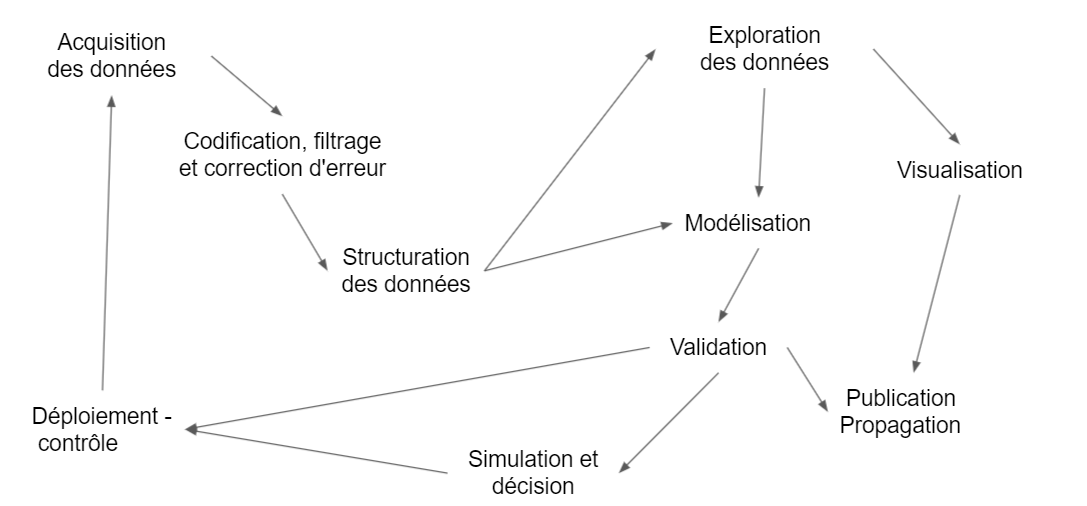
\includegraphics{./Images/datascience2.png}

\begin{itemize}
\tightlist
\item
  Acquisition
\item
  Codification , filtrage et correction d'erreur
\item
  Structuration des données : api, open data
\item
  Exploration
\item
  Modélisation :
\item
  validation : tests versus AB testing
\item
  Simulation et décision
\item
  Vizualisation et sensemaking
\item
  Déploiement :
\item
  Contrôle :
\item
  Publication : dash board, pdf , slide etc, webb site
\end{itemize}

\hypertarget{les-facteurs-de-duxe9veloppement-des-datasciences}{%
\section{Les facteurs de développement des datasciences}\label{les-facteurs-de-duxe9veloppement-des-datasciences}}

Ces développements sont favorisés par un environnement fertile dont trois facteurs se renforcent mutuellement.

\hypertarget{une-lingua-franca}{%
\subsection{Une lingua franca}\label{une-lingua-franca}}

histoire de r
histoire de python

\hypertarget{une-communautuxe9}{%
\subsection{Une communauté}\label{une-communautuxe9}}

Le second facteur , intimement lié au premier, est la constitution d'une large communauté de développeurs et d'utilisateurs qui se retrouvent aujourd'hui dans des plateformes de dépots (Github, Gitlab), de plateformes de type quora (StalkOverFlow), de tutoriaux, de blogs (BloggeR), de journaux (Journal of Statistical Software) et de bookdown.

Des ressources abondantes sont ainsi disponibles et facilitent la formation des chercheurs et des data scientists. Toutes les conditions sont réunies pour engendrer une effervescence créative.

\hypertarget{la-multiplication-des-sources-de-donnuxe9es.}{%
\subsection{La multiplication des sources de données.}\label{la-multiplication-des-sources-de-donnuxe9es.}}

Le troisième est la multiplication des sources de données et leur facilité d'accès. Les données privées, et en particulier celles des réseaux sociaux, même si un péage doit être payé pour accéder aux APIs, popularisent le traitement de données massives. Le mouvement des données ouvertes (open data) proposent et facilitent l'accès à des milliers de corps de données : retards de la SNCF, grand débat, le formidable travail de l'Insee, european survey etc.

\hypertarget{du-ml-uxe0-lia}{%
\subsection{du ML à l'IA}\label{du-ml-uxe0-lia}}

Le retour au boites noires dans les années 2000. Ce qui distingue les statistiques traditionnelles de l'approche machine learning réside d'abord par une approche de la modèlisation différente. Les modèles statistiques et économétriques considèrent non seulement une structure ( moddèle linéaires par ex), la spécification du modèle, mais aussi des modèles de distribution qui définissent le cadre d'estimation. L'évaluation passe par le test du respects des hypothèses de constructions ( distribution des erreurs), et de la qualité d'ajustement. Le machine learning, se concentre sur la valeur prédictive, et considère n'importe quelle spécification même si elle est peu intelligible et comprend de grandes quantité de paramètres.

KNN, SVM, rf et le retour des réseaux de neurones.

La révolution des convolutions et la multiplication des architectures

\hypertarget{prise-en-main}{%
\chapter{Prise en main}\label{prise-en-main}}

Pour démarrer :

1 - Télécharger et installer r sur le site du Comprehensive r Archive Network
2 - Télécharger et installer Rstudio.(version free)
3 - Dans le cadre de cet atelier, on adopte la méthode du \href{https://rmarkdown.rstudio.com/lesson-1.html}{rmarkdown}. On recommande fortement de lire l'ouvrage de référence, même si la prise en main est très rapide. Il est désormais indispensable d'utiliser le package tidyverse et en particulier les fonctions de manipulation et de pipe ( \%\textgreater\%) fournies par dplyr

\hypertarget{la-convention-du-rmarkdown}{%
\section{La convention du Rmarkdown}\label{la-convention-du-rmarkdown}}

Différentes manières d'interagir avec r sont possibles : la première est le mode console, pour de petite opérations et un utilisateur chevronné, celà peut être commode car rapide mais très rapidement on sera amené à enregistrer les opérations dans des scripts. Une idée novatrice a été d'intégrer l'ensemble des élements dans un seul document : le script découpé en petits éléments : des chunks, le commentaire et l'analyse verbabe dans un format texte, et le résultat. Dans l'univers python il s'agit des carnets Jupiter, pour r c'est le rmarkdown.

C'est un dialecte du markdown générique adapté au langage r. On recommande au lecteur d'en lire \href{https://bookdown.org/yihui/rmarkdown/}{le manuel} et de le garder dans ses onglets.

Quelques éléments de base :

un document markdown est composé de plusieurs éléments

\begin{itemize}
\tightlist
\item
  Yalm dans cet entête les éléments essentiels sont définis et paramétrés
\item
  Texte : il suit les conventions de mise en forme du html :
  ** des \# pour les niveau de titres
  ** (x){[}*.html{]} pour des liens et \includegraphics{image.jpg} pour des images
  **
\item
  Les chunks sont isolé par 3 tiks au début et à la fin.
\item
  Résultats apparaissent sous les chunks
\end{itemize}

\url{https://rmarkdown.rstudio.com/authoring_pandoc_markdown.html\#Footnotes}

Ce document peut être excécuté et publié sous différents formats : html, lpadf ou même word avec les éléments suivants
* plan
* texte
* code
* résultats
* Bibliographie
* Références
* liens
* images

\hypertarget{lire-les-donnuxe9es}{%
\section{Lire les données}\label{lire-les-donnuxe9es}}

La première étape c'est la lecture des données. On commence par le plus simple la lecture de fichiers locaux, dont les formats sont multiples : csv, tsv, xlsx, Spss, etc\ldots{} Le package readr contribue à cette tâche.

\begin{Shaded}
\begin{Highlighting}[]
\NormalTok{df <-}\StringTok{ }\KeywordTok{read_csv}\NormalTok{(}\StringTok{"./Data/BXL_listings.csv"}\NormalTok{)}
\end{Highlighting}
\end{Shaded}

Il est possible aussi d'accéder en direct aux données du web, c'est bien utile pour s'assurer que les données sont bien fraiches. Par exemple une connexion à Nsppolls qui propose une compilation de tous les sondages d'intention de vote de la présidentielle 2022.

\begin{Shaded}
\begin{Highlighting}[]
\NormalTok{df_pol <-}\StringTok{ }\KeywordTok{read_delim}\NormalTok{(}\StringTok{"https://raw.githubusercontent.com/nsppolls/nsppolls/master/presidentielle.csv"}\NormalTok{, }
                     \DataTypeTok{delim =} \StringTok{","}\NormalTok{, }\DataTypeTok{escape_double =} \OtherTok{FALSE}\NormalTok{, }\DataTypeTok{trim_ws =} \OtherTok{TRUE}\NormalTok{)}
\end{Highlighting}
\end{Shaded}

\hypertarget{la-diversituxe9-des-formats}{%
\subsection{La diversité des formats}\label{la-diversituxe9-des-formats}}

Peu de formats échappent à r, ils peuvent faire appel à des packages spécifiques

\begin{itemize}
\tightlist
\item
  excell
\item
  Json
\item
  shape et autre GIS :
\item
  les formats bibliographique : bib et ris
\end{itemize}

\hypertarget{les-autres-accuxe8s-aux-donnuxe9es}{%
\subsection{Les autres accès aux données}\label{les-autres-accuxe8s-aux-donnuxe9es}}

Interfaces

le génie des API : ne pas se soucier de la mise à jour à chaque fois qu'on lance un calcul.

exemples :

\begin{itemize}
\tightlist
\item
  base d'archive de presse
\item
  api des réseaux sociaux : tweetr
\item
  open data
\end{itemize}

\hypertarget{dplyr-pour-manipuler-les-donnuxe9es}{%
\section{\texorpdfstring{\texttt{Dplyr} pour manipuler les données}{Dplyr pour manipuler les données}}\label{dplyr-pour-manipuler-les-donnuxe9es}}

C'est un des packages essentiels de la suite tidyverse. Il permet de manipuler aisément les données et mérite une étude approfondie. Un \href{https://dplyr.tidyverse.org/articles/dplyr.html}{point de départ} ou en français : \href{http://larmarange.github.io/analyse-R/manipuler-les-donnees-avec-dplyr.html}{dplyr} .

\hypertarget{des-pipes}{%
\subsection{Des pipes \%\textgreater\%}\label{des-pipes}}

Une grand part de l'intérêt de dplyr est de reprendre un opérateur de maggritr très utiles : le pipe : \%\textgreater\%. Celui ci permet de passer le résultats de l'opération à gauche, dans la fonction de droite.

Un exemple simple . Dans la ligne de code suivante, une première fonction lit le fichier CSV, et envoie le résultat de cette lecture dans une fonction graphique élémentaire: compter le nombre d'occurences des modalité de la variable room\_type. On reviendra longuement sur ggplot, à ce stade ce qui compte c'est de retenir le procédé.

\begin{Shaded}
\begin{Highlighting}[]
\NormalTok{g <-}\StringTok{ }\KeywordTok{read_csv}\NormalTok{(}\StringTok{"./Data/BXL_listings.csv"}\NormalTok{) }\OperatorTok\StringTok{ }
\StringTok{  }\KeywordTok{ggplot}\NormalTok{(}\KeywordTok{aes}\NormalTok{(}\DataTypeTok{x=}\NormalTok{price))}\OperatorTok{+}
\StringTok{  }\KeywordTok{geom_histogram}\NormalTok{()}
\NormalTok{g}
\end{Highlighting}
\end{Shaded}

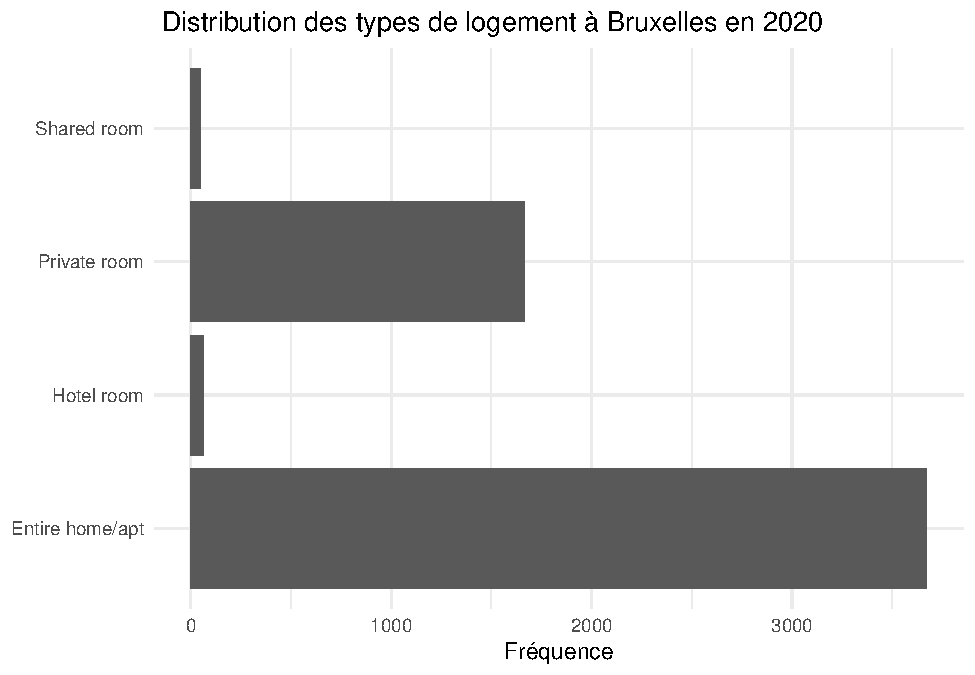
\includegraphics{bookdown-demo_files/figure-latex/0203-1.pdf}

\hypertarget{des-verbes}{%
\subsection{Des verbes}\label{des-verbes}}

L'originalité de dplyr est de définir des fonctions comme des verbes. Chaque verbe désigne un type d'action. On va les examiner progressivement :
Ils sont simples à comprendre : tansformer une variables, filter les obsersation selon un critère, isoler des variables, les groupper pour en calculer des résultats statistiqyes ( somme, moyenne, variance, max min etc) * les déployer selon un format long ou les distribuer en différents critères, les fusionner enfin selon les grandes modalité du SQL)

\hypertarget{mutate}{%
\subsubsection{Mutate}\label{mutate}}

En Français c'est ``transformer''. On modifie la valeur d'une variable par une fonction plus ou moins complexe, éventuellement en ajoutant des conditions.

Dans notre exemple, faisant au plus simple, puisque la distribution est asymétrique, une transformation du prix par les log peut donner des résultats intéressants.

Et c'est le cas. On retrouve une distribution qui semble être gaussienne.

\begin{Shaded}
\begin{Highlighting}[]
\NormalTok{g <-}\StringTok{ }\KeywordTok{read_csv}\NormalTok{(}\StringTok{"./Data/BXL_listings.csv"}\NormalTok{) }\OperatorTok\StringTok{ }
\StringTok{  }\KeywordTok{mutate}\NormalTok{(}\DataTypeTok{price=}\KeywordTok{log10}\NormalTok{(price))}\OperatorTok
\StringTok{  }\KeywordTok{ggplot}\NormalTok{(}\KeywordTok{aes}\NormalTok{(}\DataTypeTok{x=}\NormalTok{price))}\OperatorTok{+}\KeywordTok{geom_histogram}\NormalTok{()}
\NormalTok{g}
\end{Highlighting}
\end{Shaded}

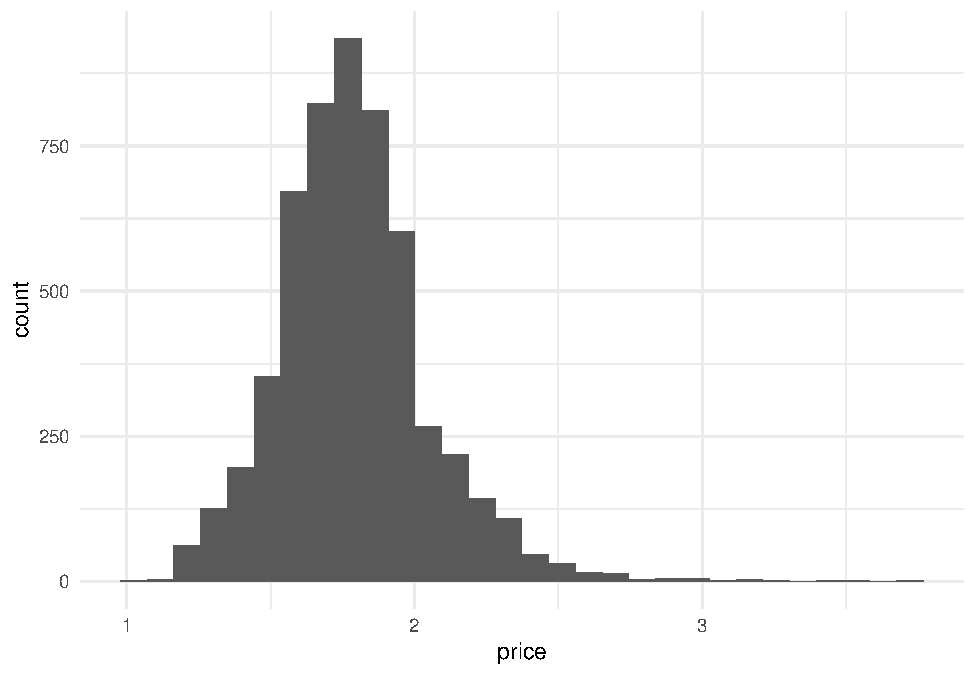
\includegraphics{bookdown-demo_files/figure-latex/0204-1.pdf}

\hypertarget{filter}{%
\subsubsection{Filter}\label{filter}}

On peut vouloir se concentrer sur une sous population. par exemple les chambres privées.

\begin{Shaded}
\begin{Highlighting}[]
\NormalTok{g <-}\StringTok{ }\KeywordTok{read_csv}\NormalTok{(}\StringTok{"./Data/BXL_listings.csv"}\NormalTok{) }\OperatorTok\StringTok{ }
\StringTok{  }\KeywordTok{filter}\NormalTok{(room_type}\OperatorTok{==}\StringTok{"Private room"}\NormalTok{)}\OperatorTok\StringTok{ }
\StringTok{  }\CommentTok{# on note que le signe == est double, c'est pour dire que la variable prend la valeur, ou non, qui est proposée}
\StringTok{  }\KeywordTok{mutate}\NormalTok{(}\DataTypeTok{price=}\KeywordTok{log10}\NormalTok{(price))}\OperatorTok
\StringTok{  }\KeywordTok{ggplot}\NormalTok{(}\KeywordTok{aes}\NormalTok{(}\DataTypeTok{x=}\NormalTok{price))}\OperatorTok{+}\KeywordTok{geom_histogram}\NormalTok{()}
\NormalTok{g}
\end{Highlighting}
\end{Shaded}

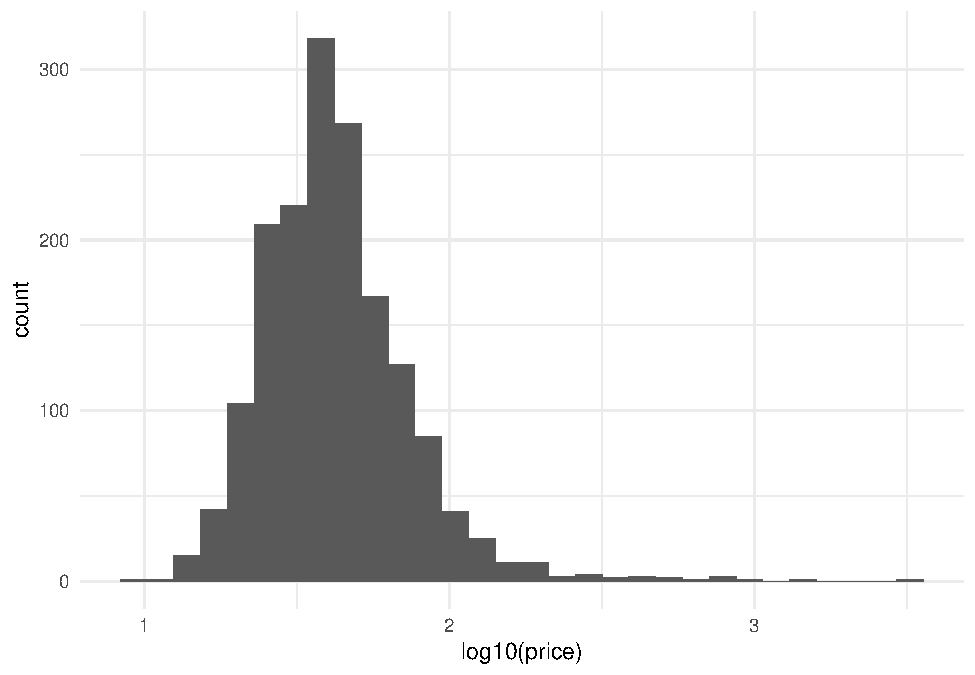
\includegraphics{bookdown-demo_files/figure-latex/0205-1.pdf}

\hypertarget{select}{%
\subsubsection{select}\label{select}}

On peut selectionner des colonnes pour créer un tableau spécifique

\begin{Shaded}
\begin{Highlighting}[]
\NormalTok{foo <-}\StringTok{ }\KeywordTok{read_csv}\NormalTok{(}\StringTok{"./Data/BXL_listings.csv"}\NormalTok{) }\OperatorTok
\StringTok{  }\NormalTok{dplyr}\OperatorTok{::}\KeywordTok{select}\NormalTok{(room_type,price) }\OperatorTok\StringTok{ }
\StringTok{  }\KeywordTok{head}\NormalTok{(}\DecValTok{5}\NormalTok{) }\CommentTok{#afficher les 5 premières observations}
\NormalTok{foo}
\end{Highlighting}
\end{Shaded}

\begin{verbatim}
## # A tibble: 5 x 2
##   room_type       price
##   <chr>           <dbl>
## 1 Entire home/apt    91
## 2 Entire home/apt    74
## 3 Hotel room        120
## 4 Entire home/apt   200
## 5 Entire home/apt    74
\end{verbatim}

\hypertarget{group_by-et-summarize}{%
\subsubsection{Group\_by et summarize}\label{group_by-et-summarize}}

c'est une opération clé, en groupant selon les modalités d'une ou pluseirs variables, on peut construire des tableaux aggrégés.On l'associera à \texttt{summarize} qui permet de calculer les statistique aggrégé selon le groupe que l'on a définit.

\begin{Shaded}
\begin{Highlighting}[]
\NormalTok{foo <-}\StringTok{ }\KeywordTok{read_csv}\NormalTok{(}\StringTok{"./Data/BXL_listings.csv"}\NormalTok{)}\OperatorTok\StringTok{ }
\StringTok{  }\NormalTok{dplyr}\OperatorTok{::}\KeywordTok{select}\NormalTok{(neighbourhood, price)}\OperatorTok
\StringTok{    }\KeywordTok{group_by}\NormalTok{(neighbourhood ) }\OperatorTok\StringTok{ }
\StringTok{  }\KeywordTok{summarise}\NormalTok{(}\DataTypeTok{averageprice=}\KeywordTok{mean}\NormalTok{(price)) }

\KeywordTok{head}\NormalTok{(foo, }\DecValTok{5}\NormalTok{)}
\end{Highlighting}
\end{Shaded}

\begin{verbatim}
## # A tibble: 5 x 2
##   neighbourhood         averageprice
##   <chr>                        <dbl>
## 1 Anderlecht                    71.9
## 2 Auderghem                     66.3
## 3 Berchem-Sainte-Agathe         65.9
## 4 Bruxelles                     91.0
## 5 Etterbeek                     75.8
\end{verbatim}

\hypertarget{pivot_wider-et-pivot_longer}{%
\subsubsection{Pivot\_wider et pivot\_longer}\label{pivot_wider-et-pivot_longer}}

Si pour l'habitué des feuilles excell les données croisent des observations avec des variables, ce format n'est pas le seul moyen de réprésenter des données, et pas forcément le meilleur.

\begin{figure}
\centering
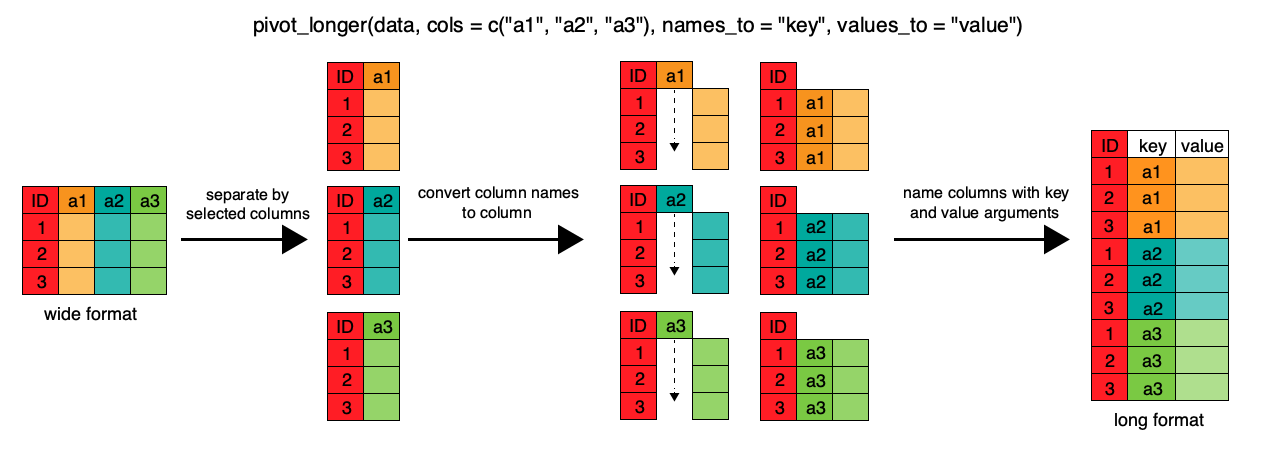
\includegraphics{./Images/pivot_longer.png}
\caption{merge}
\end{figure}

\begin{figure}
\centering
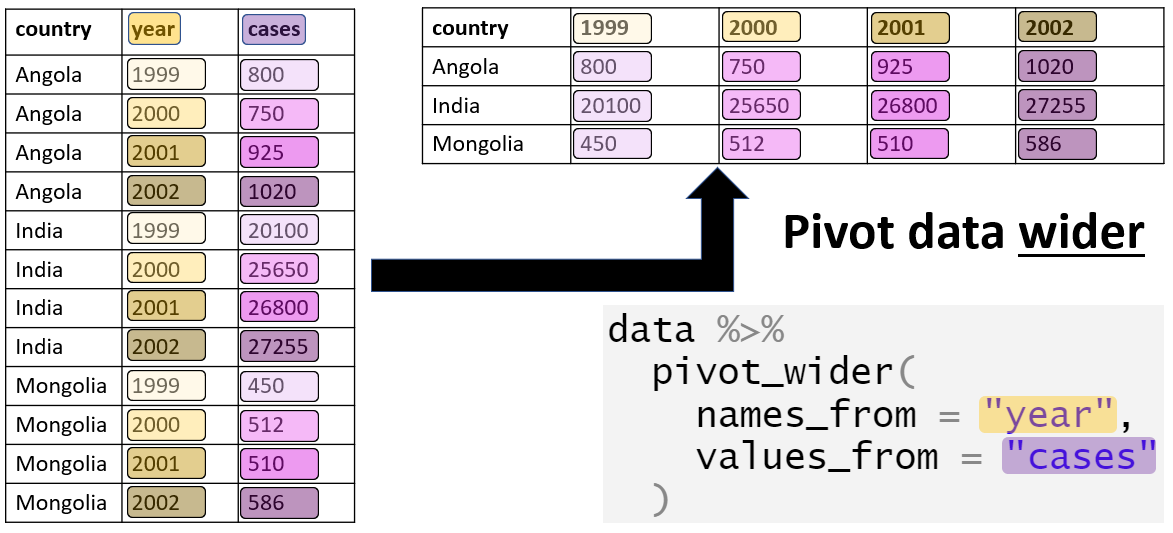
\includegraphics{./Images/pivot_wider.png}
\caption{merge}
\end{figure}

\hypertarget{merge}{%
\subsubsection{merge}\label{merge}}

On sera souvent amené à fabriquer des tableaux de donnée en les enrichissant d'un autre. On sera amené à fusionner les données.

Le cas le plus simples est d'ajouter d'autres observation à un fichier de données, si les variables sont identitiques on peut concaténer diffrents jeux de données avec la fonction de base rbind au contraire si les observation sont les mêmes, et que seules les variables sont différentes on peut utiliser cbind. L'équivalent de DPLYR est row\_bind et column\_bind

mais très souvent on sera dans des cas différents et la fusion des données devra suivre des index

\begin{figure}
\centering
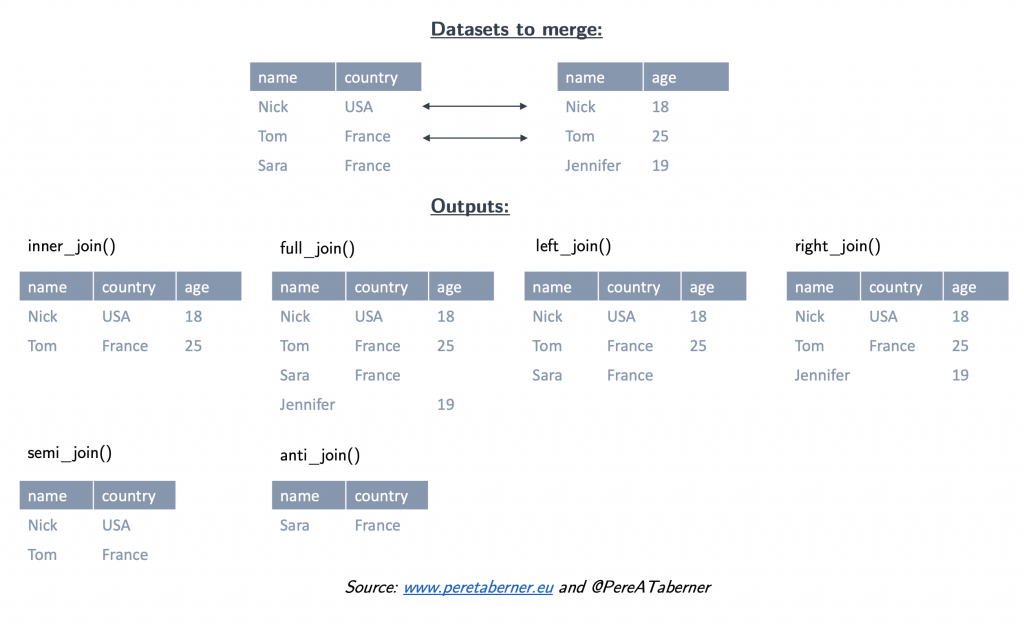
\includegraphics{./Images/merge_ex-1024x624.png}
\caption{merge}
\end{figure}

quatre types de fusion

genérale

fusion à gauche

fusion à droite

\url{https://coletl.github.io/tidy_intro/lessons/dplyr_join/dplyr_join.html}

\hypertarget{pour-aller-plus-loin}{%
\section{Pour aller plus loin}\label{pour-aller-plus-loin}}

On engage le lecteur à poursuivre avec

\begin{itemize}
\tightlist
\item
  le bookdown au-delà du markdown
\item
  une théorie des tidy data
\end{itemize}

\hypertarget{analyses-univariuxe9es}{%
\chapter{Analyses univariées}\label{analyses-univariuxe9es}}

Nous avons appris à lire des données, à les manipuler, nous avons le droit d'être pressé de les représenter de manière immédiatement lisible, par des dataviz.

On présente d'abord rapidement le concept de grammaire des graphiques

On se concentre ensuite sur un cas d'étude

On décline.

\hypertarget{la-grammaire-des-graphiques}{%
\section{La grammaire des graphiques}\label{la-grammaire-des-graphiques}}

C'est sans doute une des percées conceptuelles laplus intéressante des datasciences. La représentation graphhiques des données fait l'objet à la fois d'une explosion créative mais aussi d'une synthèse théorique. C'est l'apport de la grammaire des graphiques.

Ces outils s'appuient sur l'idée de \href{https://www.goodreads.com/book/show/2549408.The_Grammar_of_Graphics}{grammaire des graphiques}. En voici un \href{https://cfss.uchicago.edu/notes/grammar-of-graphics/}{clair résumé}.En français il y a toujours le \href{http://larmarange.github.io/analyse-R/intro-ggplot2.html}{larmarange}

\hypertarget{un-moduxe8le-en-couche}{%
\subsection{Un modèle en couche}\label{un-moduxe8le-en-couche}}

Celle-ci met un ordre dans les éléments qui composent un graphique et les superpose.

\begin{figure}
\centering

\includegraphics{./Images/graphiclayers.png}
\caption{layers}
\end{figure}

\begin{itemize}
\tightlist
\item
  l'aesthetic definit les éléments que l'on veut représenter : ce qu'on met en abscisse, ce qu'on met en ordonnné, les groupes que l'on veut distinguer.
\item
  la geométrie (geom\_x)qui définit la forme de représentation
\item
  les échelles (scale\_x)
\item
  Labelisation (labs)
\item
  les templates
\item
  le facetting
\end{itemize}

ggplot est construit selon cette structure. Voici le \href{https://ggplot2-book.org/}{book de référence}, qui est au centre de ce cours. On aura besoin de manière assez systématique de manipuler les données avant de les représenter, \href{http://larmarange.github.io/analyse-R/manipuler-les-donnees-avec-dplyr.html}{dplyr} nous permet de le faire aisément.

\hypertarget{une-typologie-des-repruxe9sentations}{%
\subsection{Une typologie des représentations}\label{une-typologie-des-repruxe9sentations}}

Un point de départ fondamental est la \href{https://www.r-graph-gallery.com/}{gallery de ggplot},, elle présente de manière synthétique la plupart les types de figures qui peuvent être représentées, avec du code facilement reproductible.

Une classification simple

\begin{itemize}
\tightlist
\item
  Analyse univariée
\item
  Analyse bi variée
\item
  Analyse multivariée
  ** les variables sont quantitatives : on analyse des matrices de corrélations
  ** les variables sont qualitatives : on analyse des tableaux croisés
\item
  Analyse geospatiale
\item
  Analyse de réseaux
\item
  analyse d'arbres
\item
  Diagramme de flux
\end{itemize}

\hypertarget{lesthuxe9tique}{%
\subsection{L'esthétique}\label{lesthuxe9tique}}

L'art des couleurs tient dans les palettes on aimera celles de Wes Anderson, on peut adorer fishualize. on trouvera

\hypertarget{une-uxe9tude-de-cas}{%
\section{Une étude de cas}\label{une-uxe9tude-de-cas}}

Les données sont extraites de l'ESS, une sélection est disponible \href{}{ici}. Elle couvre les 9 vagues et concernent la France et L'Allemagne. Les variables dépendantes (celles que l'on veut étudier et expliquer) sont les 9 items de la confiance, les variable considérées comme indépendantes (ou explicatives) sont une sélection de variables socio-démographiques : âge, genre, perception du pouvoir d'achat, orientation politique, type d'habitat.

On fait quelques opérations de recodage et on renomme les variables avoir une lecture plus aisée des variables et de leurs catégories. Le plan de recodage d'un jeu de données qu'on va employer dans les chapitres suivants. Il s'appuie sur le langage de base.

L'analyse univarié, comme son nom l'indique, ne s'intéresse qu'à une seule variable. Celle-ci peut être \textbf{quantitative} ou \textbf{qualitative} etne comporter qu'un nombre limité de modalités entre lesquels aucune comparaison de grandeur ne peut être faite. Les premières ont le plus souvent dans r un format numeric, les autres correspondent au format \emph{factor}.

(Un exercice peut être de le réécrire avec dplyr.)

\begin{Shaded}
\begin{Highlighting}[]
\NormalTok{df<-}\KeywordTok{readRDS}\NormalTok{(}\StringTok{"./data/trustFrAll.rds"}\NormalTok{)}

\CommentTok{#quelques recodages}
\CommentTok{#on renomme pour plus de clarte}
\KeywordTok{names}\NormalTok{(df)[}\KeywordTok{names}\NormalTok{(df)}\OperatorTok{==}\StringTok{"trstun"}\NormalTok{] <-}\StringTok{ "NationsUnies"} 
\KeywordTok{names}\NormalTok{(df)[}\KeywordTok{names}\NormalTok{(df)}\OperatorTok{==}\StringTok{"trstep"}\NormalTok{] <-}\StringTok{ "ParlementEurop"} 
\KeywordTok{names}\NormalTok{(df)[}\KeywordTok{names}\NormalTok{(df)}\OperatorTok{==}\StringTok{"trstlgl"}\NormalTok{] <-}\StringTok{ "Justice"} 
\KeywordTok{names}\NormalTok{(df)[}\KeywordTok{names}\NormalTok{(df)}\OperatorTok{==}\StringTok{"trstplc"}\NormalTok{] <-}\StringTok{ "Police"} 
\KeywordTok{names}\NormalTok{(df)[}\KeywordTok{names}\NormalTok{(df)}\OperatorTok{==}\StringTok{"trstplt"}\NormalTok{] <-}\StringTok{ "Politiques"} 
\KeywordTok{names}\NormalTok{(df)[}\KeywordTok{names}\NormalTok{(df)}\OperatorTok{==}\StringTok{"trstprl"}\NormalTok{] <-}\StringTok{"Parlement"} 
\KeywordTok{names}\NormalTok{(df)[}\KeywordTok{names}\NormalTok{(df)}\OperatorTok{==}\StringTok{"trstprt"}\NormalTok{] <-}\StringTok{ "Partis"}
\KeywordTok{names}\NormalTok{(df)[}\KeywordTok{names}\NormalTok{(df)}\OperatorTok{==}\StringTok{"pplhlp"}\NormalTok{] <-}\StringTok{ "help"}
\KeywordTok{names}\NormalTok{(df)[}\KeywordTok{names}\NormalTok{(df)}\OperatorTok{==}\StringTok{"pplfair"}\NormalTok{] <-}\StringTok{ "fair"}
\KeywordTok{names}\NormalTok{(df)[}\KeywordTok{names}\NormalTok{(df)}\OperatorTok{==}\StringTok{"ppltrst"}\NormalTok{] <-}\StringTok{ "trust"}

\CommentTok{#on construit les scores de confiance }
\NormalTok{df<-df }\OperatorTok\StringTok{ }
\StringTok{  }\KeywordTok{mutate}\NormalTok{(}\DataTypeTok{trust_institut=}\NormalTok{(Partis}\OperatorTok{+}\NormalTok{Parlement}\OperatorTok{+}\NormalTok{Politiques}\OperatorTok{+}\NormalTok{Police}\OperatorTok{+}\NormalTok{Justice}\OperatorTok{+}\NormalTok{NationsUnies}\OperatorTok{+}\NormalTok{ParlementEurop)}\OperatorTok{*}\DecValTok{10}\OperatorTok{/}\DecValTok{7}\NormalTok{,}\DataTypeTok{trust_interpersonnel=}\NormalTok{(help}\OperatorTok{+}\NormalTok{fair}\OperatorTok{+}\NormalTok{trust)}\OperatorTok{*}\DecValTok{10}\OperatorTok{/}\DecValTok{3}\NormalTok{)}
\NormalTok{df}\OperatorTok{$}\NormalTok{Year<-}\DecValTok{2000}
\CommentTok{#recodage des variables independantes}
\NormalTok{df}\OperatorTok{$}\NormalTok{Year[df}\OperatorTok{$}\NormalTok{essround}\OperatorTok{==}\DecValTok{1}\NormalTok{]<-}\DecValTok{2002}
\NormalTok{df}\OperatorTok{$}\NormalTok{Year[df}\OperatorTok{$}\NormalTok{essround}\OperatorTok{==}\DecValTok{2}\NormalTok{]<-}\DecValTok{2004}
\NormalTok{df}\OperatorTok{$}\NormalTok{Year[df}\OperatorTok{$}\NormalTok{essround}\OperatorTok{==}\DecValTok{3}\NormalTok{]<-}\DecValTok{2006}
\NormalTok{df}\OperatorTok{$}\NormalTok{Year[df}\OperatorTok{$}\NormalTok{essround}\OperatorTok{==}\DecValTok{4}\NormalTok{]<-}\DecValTok{2008}
\NormalTok{df}\OperatorTok{$}\NormalTok{Year[df}\OperatorTok{$}\NormalTok{essround}\OperatorTok{==}\DecValTok{5}\NormalTok{]<-}\DecValTok{2010}
\NormalTok{df}\OperatorTok{$}\NormalTok{Year[df}\OperatorTok{$}\NormalTok{essround}\OperatorTok{==}\DecValTok{6}\NormalTok{]<-}\DecValTok{2012}
\NormalTok{df}\OperatorTok{$}\NormalTok{Year[df}\OperatorTok{$}\NormalTok{essround}\OperatorTok{==}\DecValTok{7}\NormalTok{]<-}\DecValTok{2014}
\NormalTok{df}\OperatorTok{$}\NormalTok{Year[df}\OperatorTok{$}\NormalTok{essround}\OperatorTok{==}\DecValTok{8}\NormalTok{]<-}\DecValTok{2016}
\NormalTok{df}\OperatorTok{$}\NormalTok{Year[df}\OperatorTok{$}\NormalTok{essround}\OperatorTok{==}\DecValTok{9}\NormalTok{]<-}\DecValTok{2018}
\NormalTok{df}\OperatorTok{$}\NormalTok{Year<-}\KeywordTok{as.factor}\NormalTok{(df}\OperatorTok{$}\NormalTok{Year) }

\NormalTok{df}\OperatorTok{$}\NormalTok{OP<-}\StringTok{" "}
\CommentTok{#ggplot(df,aes(x=lrscale))+geom_histogram()}
\NormalTok{df}\OperatorTok{$}\NormalTok{OP[df}\OperatorTok{$}\NormalTok{lrscale}\OperatorTok{==}\DecValTok{0}\NormalTok{] <-}\StringTok{ "Extrême gauche"} 
\NormalTok{df}\OperatorTok{$}\NormalTok{OP[df}\OperatorTok{$}\NormalTok{lrscale}\OperatorTok{==}\DecValTok{1}\NormalTok{] <-}\StringTok{ "Gauche"} 
\NormalTok{df}\OperatorTok{$}\NormalTok{OP[df}\OperatorTok{$}\NormalTok{lrscale}\OperatorTok{==}\DecValTok{2}\NormalTok{] <-}\StringTok{ "Gauche"} 
\NormalTok{df}\OperatorTok{$}\NormalTok{OP[df}\OperatorTok{$}\NormalTok{lrscale}\OperatorTok{==}\DecValTok{3}\NormalTok{] <-}\StringTok{ "Centre Gauche"} 
\NormalTok{df}\OperatorTok{$}\NormalTok{OP[df}\OperatorTok{$}\NormalTok{lrscale}\OperatorTok{==}\DecValTok{4}\NormalTok{] <-}\StringTok{ "Centre Gauche"} 
\NormalTok{df}\OperatorTok{$}\NormalTok{OP[df}\OperatorTok{$}\NormalTok{lrscale}\OperatorTok{==}\DecValTok{5}\NormalTok{] <-}\StringTok{ "Ni G ni D"} 
\NormalTok{df}\OperatorTok{$}\NormalTok{OP[df}\OperatorTok{$}\NormalTok{lrscale}\OperatorTok{==}\DecValTok{6}\NormalTok{] <-}\StringTok{ "Centre Droit"} 
\NormalTok{df}\OperatorTok{$}\NormalTok{OP[df}\OperatorTok{$}\NormalTok{lrscale}\OperatorTok{==}\DecValTok{7}\NormalTok{] <-}\StringTok{ "Centre Droit"} 
\NormalTok{df}\OperatorTok{$}\NormalTok{OP[df}\OperatorTok{$}\NormalTok{lrscale}\OperatorTok{==}\DecValTok{8}\NormalTok{] <-}\StringTok{ "Droite"} 
\NormalTok{df}\OperatorTok{$}\NormalTok{OP[df}\OperatorTok{$}\NormalTok{lrscale}\OperatorTok{==}\DecValTok{9}\NormalTok{] <-}\StringTok{ "Droite"} 
\NormalTok{df}\OperatorTok{$}\NormalTok{OP[df}\OperatorTok{$}\NormalTok{lrscale}\OperatorTok{==}\DecValTok{10}\NormalTok{] <-}\StringTok{ "Extrême droite"} 
\CommentTok{#la ligne suivante est pour ordonner les modalités de la variables}
\NormalTok{df}\OperatorTok{$}\NormalTok{OP<-}\KeywordTok{factor}\NormalTok{(df}\OperatorTok{$}\NormalTok{OP,}\DataTypeTok{levels=}\KeywordTok{c}\NormalTok{(}\StringTok{"Extrême droite"}\NormalTok{,}\StringTok{"Droite"}\NormalTok{,}\StringTok{"Centre Droit"}\NormalTok{,}\StringTok{"Ni G ni D"}\NormalTok{,}\StringTok{"Centre Gauche"}\NormalTok{,}\StringTok{"Gauche"}\NormalTok{,}\StringTok{"Extrême gauche"}\NormalTok{))}


\NormalTok{df}\OperatorTok{$}\NormalTok{revenu<-}\StringTok{" "}
\NormalTok{df}\OperatorTok{$}\NormalTok{revenu[df}\OperatorTok{$}\NormalTok{hincfel}\OperatorTok{>}\DecValTok{4}\NormalTok{] <-}\StringTok{ }\OtherTok{NA}
\NormalTok{df}\OperatorTok{$}\NormalTok{revenu[df}\OperatorTok{$}\NormalTok{hincfel}\OperatorTok{==}\DecValTok{1}\NormalTok{] <-}\StringTok{ "Vie confortable"} 
\NormalTok{df}\OperatorTok{$}\NormalTok{revenu[df}\OperatorTok{$}\NormalTok{hincfel}\OperatorTok{==}\DecValTok{2}\NormalTok{] <-}\StringTok{ "Se débrouille avec son revenu"} 
\NormalTok{df}\OperatorTok{$}\NormalTok{revenu[df}\OperatorTok{$}\NormalTok{hincfel}\OperatorTok{==}\DecValTok{3}\NormalTok{] <-}\StringTok{ "Revenu insuffisant"} 
\NormalTok{df}\OperatorTok{$}\NormalTok{revenu[df}\OperatorTok{$}\NormalTok{hincfel}\OperatorTok{==}\DecValTok{4}\NormalTok{] <-}\StringTok{ "Revenu très insuffisant"} 
\NormalTok{df}\OperatorTok{$}\NormalTok{revenu<-}\KeywordTok{factor}\NormalTok{(df}\OperatorTok{$}\NormalTok{revenu,}\DataTypeTok{levels=}\KeywordTok{c}\NormalTok{(}\StringTok{"Vie confortable"}\NormalTok{,}\StringTok{"Se débrouille avec son revenu"}\NormalTok{,}\StringTok{"Revenu insuffisant"}\NormalTok{,}\StringTok{"Revenu très insuffisant"}\NormalTok{))}

\NormalTok{df}\OperatorTok{$}\NormalTok{habitat<-}\StringTok{" "}

\NormalTok{df}\OperatorTok{$}\NormalTok{habitat[df}\OperatorTok{$}\NormalTok{domicil}\OperatorTok{==}\DecValTok{1}\NormalTok{]<-}\StringTok{ "Big city"}
\NormalTok{df}\OperatorTok{$}\NormalTok{habitat[df}\OperatorTok{$}\NormalTok{domicil}\OperatorTok{==}\DecValTok{2}\NormalTok{]<-}\StringTok{"Suburbs"}
\NormalTok{df}\OperatorTok{$}\NormalTok{habitat[df}\OperatorTok{$}\NormalTok{domicil}\OperatorTok{==}\DecValTok{3}\NormalTok{]<-}\StringTok{"Town"}
\NormalTok{df}\OperatorTok{$}\NormalTok{habitat[df}\OperatorTok{$}\NormalTok{domicil}\OperatorTok{==}\DecValTok{4}\NormalTok{]<-}\StringTok{"Village"}
\NormalTok{df}\OperatorTok{$}\NormalTok{habitat[df}\OperatorTok{$}\NormalTok{domicil}\OperatorTok{==}\DecValTok{5}\NormalTok{]<-}\StringTok{"Countryside"}
\NormalTok{df}\OperatorTok{$}\NormalTok{habitat<-}\KeywordTok{factor}\NormalTok{(df}\OperatorTok{$}\NormalTok{habitat,}\DataTypeTok{levels=}\KeywordTok{c}\NormalTok{(}\StringTok{"Big city"}\NormalTok{,}\StringTok{"Suburbs"}\NormalTok{,}\StringTok{"Town"}\NormalTok{,}\StringTok{"Village"}\NormalTok{,}\StringTok{"Countryside"}\NormalTok{))}

\NormalTok{df}\OperatorTok{$}\NormalTok{genre<-}\StringTok{" "}

\NormalTok{df}\OperatorTok{$}\NormalTok{genre[df}\OperatorTok{$}\NormalTok{gndr}\OperatorTok{==}\DecValTok{1}\NormalTok{]<-}\StringTok{"H"}
\NormalTok{df}\OperatorTok{$}\NormalTok{genre[df}\OperatorTok{$}\NormalTok{gndr}\OperatorTok{==}\DecValTok{2}\NormalTok{]<-}\StringTok{"F"}

\NormalTok{df}\OperatorTok{$}\NormalTok{age<-}\StringTok{" "}

\NormalTok{df}\OperatorTok{$}\NormalTok{age[df}\OperatorTok{$}\NormalTok{agea}\OperatorTok{<}\DecValTok{26}\NormalTok{]<-}\StringTok{"25<"}
\NormalTok{df}\OperatorTok{$}\NormalTok{age[df}\OperatorTok{$}\NormalTok{agea}\OperatorTok{>}\DecValTok{25} \OperatorTok{&}\StringTok{ }\NormalTok{df}\OperatorTok{$}\NormalTok{agea}\OperatorTok{<}\DecValTok{36}\NormalTok{]<-}\StringTok{"26-35"}
\NormalTok{df}\OperatorTok{$}\NormalTok{age[df}\OperatorTok{$}\NormalTok{agea}\OperatorTok{>}\DecValTok{35} \OperatorTok{&}\StringTok{ }\NormalTok{df}\OperatorTok{$}\NormalTok{agea}\OperatorTok{<}\DecValTok{46}\NormalTok{]<-}\StringTok{"36-45"}
\NormalTok{df}\OperatorTok{$}\NormalTok{age[df}\OperatorTok{$}\NormalTok{agea}\OperatorTok{>}\DecValTok{45} \OperatorTok{&}\StringTok{ }\NormalTok{df}\OperatorTok{$}\NormalTok{agea}\OperatorTok{<}\DecValTok{66}\NormalTok{]<-}\StringTok{"46-65"}
\NormalTok{df}\OperatorTok{$}\NormalTok{age[df}\OperatorTok{$}\NormalTok{agea}\OperatorTok{>}\DecValTok{65} \OperatorTok{&}\StringTok{ }\NormalTok{df}\OperatorTok{$}\NormalTok{agea}\OperatorTok{<}\DecValTok{76}\NormalTok{]<-}\StringTok{"66-75"}
\NormalTok{df}\OperatorTok{$}\NormalTok{age[df}\OperatorTok{$}\NormalTok{agea}\OperatorTok{>}\DecValTok{75}\NormalTok{]<-}\StringTok{"75>"}
\NormalTok{df}\OperatorTok{$}\NormalTok{age<-}\KeywordTok{factor}\NormalTok{(df}\OperatorTok{$}\NormalTok{age,}\DataTypeTok{levels=}\KeywordTok{c}\NormalTok{(}\StringTok{"25<"}\NormalTok{,}\StringTok{"26-35"}\NormalTok{,}\StringTok{"36-45"}\NormalTok{,}\StringTok{"46-65"}\NormalTok{,}\StringTok{"66-75"}\NormalTok{, }\StringTok{"75>"}\NormalTok{))}

\KeywordTok{saveRDS}\NormalTok{(df, }\StringTok{"./data/dfTrust.rds)"}\NormalTok{)}

\NormalTok{foo<-df}\OperatorTok
\StringTok{  }\NormalTok{dplyr}\OperatorTok{::}\KeywordTok{select}\NormalTok{(Year,cntry, trust_institut, trust_interpersonnel)}\OperatorTok
\StringTok{  }\KeywordTok{group_by}\NormalTok{(Year,cntry)}\OperatorTok
\StringTok{  }\KeywordTok{summarise}\NormalTok{(}\DataTypeTok{trust_institut=}\KeywordTok{mean}\NormalTok{(trust_institut, }\DataTypeTok{na.rm=}\OtherTok{TRUE}\NormalTok{), }
            \DataTypeTok{trust_interpersonnel=}\KeywordTok{mean}\NormalTok{(trust_interpersonnel, }\DataTypeTok{na.rm=}\OtherTok{TRUE}\NormalTok{))}
\NormalTok{foo}\OperatorTok{$}\NormalTok{Year<-}\StringTok{ }\KeywordTok{as.character}\NormalTok{(foo}\OperatorTok{$}\NormalTok{Year)}
\NormalTok{foo}\OperatorTok{$}\NormalTok{cntry<-}\StringTok{ }\KeywordTok{as.character}\NormalTok{(foo}\OperatorTok{$}\NormalTok{cntry)}

\NormalTok{foo<-foo}\OperatorTok\KeywordTok{pivot_longer}\NormalTok{(}\OperatorTok{!}\KeywordTok{c}\NormalTok{(Year,cntry),}\DataTypeTok{names_to=}\StringTok{"Trust"}\NormalTok{, }\DataTypeTok{values_to=}\StringTok{"value"}\NormalTok{ )}


\KeywordTok{ggplot}\NormalTok{(foo,}\KeywordTok{aes}\NormalTok{(}\DataTypeTok{x=}\NormalTok{Year, }\DataTypeTok{y=}\NormalTok{value, }\DataTypeTok{group=}\NormalTok{Trust))}\OperatorTok{+}
\StringTok{  }\KeywordTok{geom_line}\NormalTok{(}\DataTypeTok{stat=}\StringTok{"identity"}\NormalTok{,}\KeywordTok{aes}\NormalTok{(}\DataTypeTok{color=}\NormalTok{Trust), }\DataTypeTok{size=}\FloatTok{1.2}\NormalTok{)}\OperatorTok{+}
\StringTok{  }\KeywordTok{facet_wrap}\NormalTok{(}\KeywordTok{vars}\NormalTok{(cntry))}\OperatorTok{+}
\StringTok{  }\KeywordTok{scale_color_manual}\NormalTok{(}\DataTypeTok{values =} \KeywordTok{c}\NormalTok{(}\StringTok{"Cyan3"}\NormalTok{,}\StringTok{"Orange2"}\NormalTok{))}\OperatorTok{+}\StringTok{ }\KeywordTok{theme}\NormalTok{(}
    \DataTypeTok{legend.position =} \StringTok{"bottom"}\NormalTok{,}
    \DataTypeTok{legend.justification =} \KeywordTok{c}\NormalTok{(}\StringTok{"right"}\NormalTok{, }\StringTok{"top"}\NormalTok{),}
    \DataTypeTok{legend.box.just =} \StringTok{"right"}\NormalTok{,}
    \DataTypeTok{legend.margin =} \KeywordTok{margin}\NormalTok{(}\DecValTok{6}\NormalTok{, }\DecValTok{6}\NormalTok{, }\DecValTok{6}\NormalTok{, }\DecValTok{6}\NormalTok{)}
\NormalTok{    )}\OperatorTok{+}\StringTok{ }\KeywordTok{labs}\NormalTok{(}\DataTypeTok{x=}\OtherTok{NULL}\NormalTok{, }\DataTypeTok{y=}\StringTok{"Niveau"}\NormalTok{)}\OperatorTok{+}\KeywordTok{ylim}\NormalTok{(}\DecValTok{40}\NormalTok{,}\DecValTok{60}\NormalTok{)}
\end{Highlighting}
\end{Shaded}

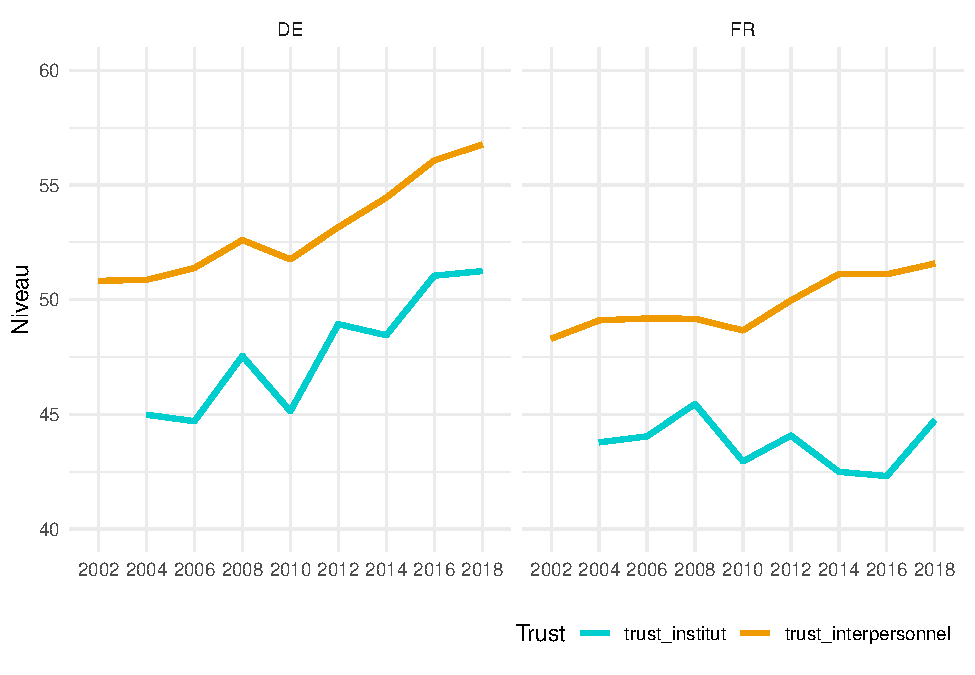
\includegraphics{bookdown-demo_files/figure-latex/301-1.pdf}

\hypertarget{le-cas-des-variables-quantitatives}{%
\subsection{Le cas des variables quantitatives}\label{le-cas-des-variables-quantitatives}}

Les variables quantitatives décrivent une variable dont les valeurs décrivent les quantités d'une grandeur. Elle peuvent être discrètes (dénombrement du d'un nombre d'unités) - le nombre d'habitant), ou continue (le nombre de km parcourus). l'\textbf{histogramme} est l'outil de base pour représenter la distribution d'une telle variable. Il représente pour des intervalles de valeurs donnés, la fréquence des observations.

Sa syntaxe simple comporte d'abord la définition de la variable et de la source de données, puis une des ``géométrie'' de ggplot : la fonction geom\_histogram. Dans notre exemple, on va représenter le score de confiance institutionnelle pour la France en se concentrant sur la dernière vague d'enquête.

\begin{Shaded}
\begin{Highlighting}[]
\CommentTok{#On charge le fichier recodé à la fin du chapitre précédent}
\NormalTok{df<-}\KeywordTok{readRDS}\NormalTok{(}\StringTok{"./data/dfTrust.rds)"}\NormalTok{)}

\CommentTok{#filtrage sur 2018 et la France.}

\NormalTok{foo<-df}\OperatorTok
\StringTok{  }\KeywordTok{filter}\NormalTok{(Year}\OperatorTok{==}\StringTok{"2018"} \OperatorTok{&}\StringTok{ }\NormalTok{cntry}\OperatorTok{==}\StringTok{"FR"} \OperatorTok{&}\StringTok{ }\OperatorTok{!}\KeywordTok{is.na}\NormalTok{(trust_institut)) }

\CommentTok{# on stocke le diagramme dans l'objet g00, pour le réutiliser ultérieurement et pouvoir le compléter.}
\NormalTok{g00<-}\KeywordTok{ggplot}\NormalTok{(foo,}\KeywordTok{aes}\NormalTok{(}\DataTypeTok{x=}\NormalTok{trust_institut))}\OperatorTok{+}
\StringTok{  }\KeywordTok{geom_histogram}\NormalTok{()}

\NormalTok{g00}
\end{Highlighting}
\end{Shaded}

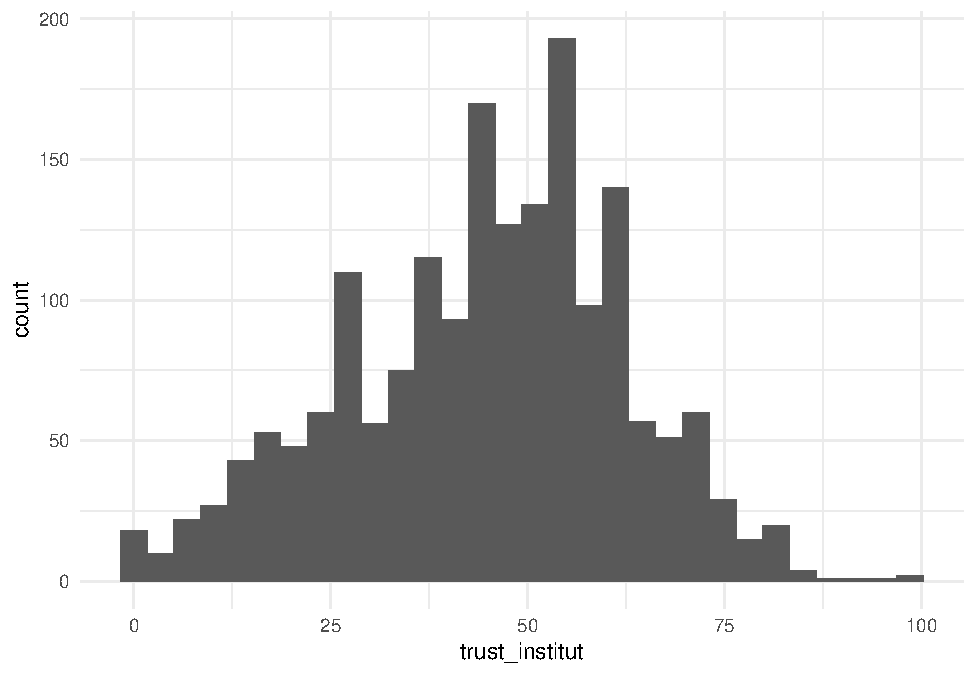
\includegraphics{bookdown-demo_files/figure-latex/302-1.pdf}

\begin{Shaded}
\begin{Highlighting}[]
\NormalTok{g00}\OperatorTok{+}\KeywordTok{labs}\NormalTok{(}\DataTypeTok{title=}\StringTok{"Distribution de la confiance institutionnelle en France et en 2018"}\NormalTok{,}
         \DataTypeTok{x=}\StringTok{"Confiance institutionnelle"}\NormalTok{)}
\end{Highlighting}
\end{Shaded}

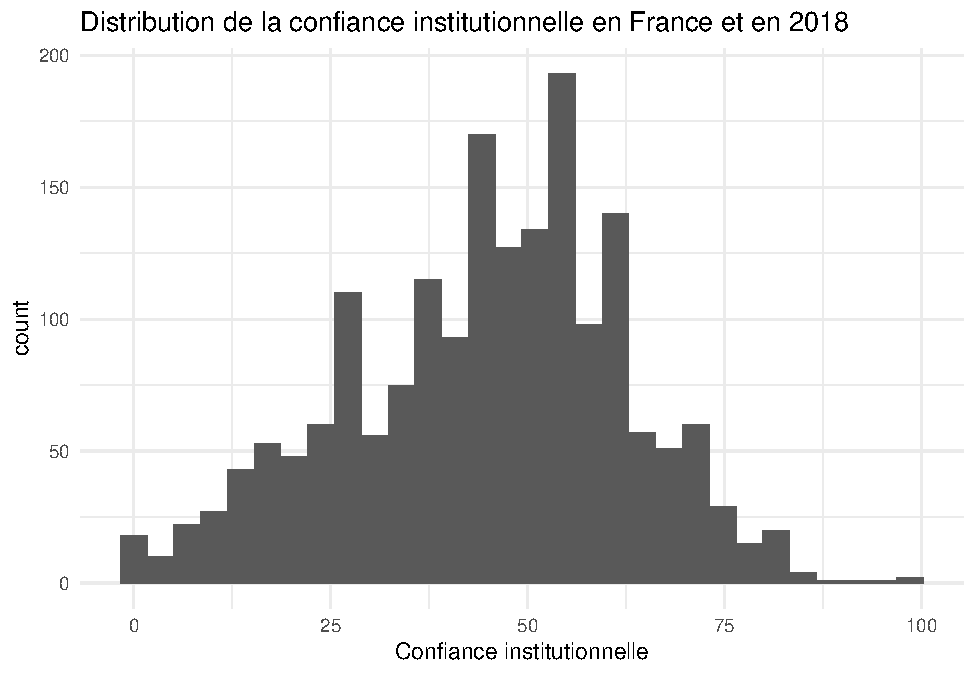
\includegraphics{bookdown-demo_files/figure-latex/302-2.pdf}

On va améliorer l'aspect en

\begin{enumerate}
\def\labelenumi{\alph{enumi})}
\tightlist
\item
  modifiant la couleur et la largeur des barres,
\item
  ajoutant un thème,
\item
  en précisant les éléments textuels (titres, label)
\item
  en calculant et en représentant la valeur moyenne et l'écart-type . Pour ces statistiques, on emploie les fonction de base : mean, sd et round.
\end{enumerate}

On notera que le titre est défini par la concaténation de plusieurs chaines de caractères avec la fonction paste0. On peut ainsi injecter dans le graphique des éléments externes au jeu de données.

\begin{Shaded}
\begin{Highlighting}[]
\CommentTok{#on calcule la moyenne}
\NormalTok{moy=}\KeywordTok{mean}\NormalTok{(foo}\OperatorTok{$}\NormalTok{trust_institut, }\DataTypeTok{na.rm=}\OtherTok{TRUE}\NormalTok{)}
\NormalTok{sd=}\KeywordTok{sd}\NormalTok{(foo}\OperatorTok{$}\NormalTok{trust_institut, }\DataTypeTok{na.rm=}\OtherTok{TRUE}\NormalTok{)}

\CommentTok{#avec tous les éléments}
\NormalTok{g01 <-}\KeywordTok{ggplot}\NormalTok{(foo,}\KeywordTok{aes}\NormalTok{(}\DataTypeTok{x=}\NormalTok{trust_institut))}\OperatorTok{+}
\StringTok{  }\KeywordTok{geom_histogram}\NormalTok{(}\DataTypeTok{binwidth=}\DecValTok{5}\NormalTok{,}\DataTypeTok{fill=}\StringTok{"pink"}\NormalTok{)}\OperatorTok{+}
\StringTok{  }\KeywordTok{labs}\NormalTok{(}\DataTypeTok{title=} \StringTok{"Distribution de la confiance institutionnelle"}\NormalTok{, }
       \DataTypeTok{subtitle=} \KeywordTok{paste0}\NormalTok{(}\StringTok{"moyenne = "}\NormalTok{,}\KeywordTok{round}\NormalTok{(moy,}\DecValTok{2}\NormalTok{), }\StringTok{" ecart-type = "}\NormalTok{, }\KeywordTok{round}\NormalTok{(sd,}\DecValTok{2}\NormalTok{)),}
       \DataTypeTok{caption=}\StringTok{"ESS2002-2018"}\NormalTok{,}
       \DataTypeTok{y=} \StringTok{"frequence"}\NormalTok{,}
       \DataTypeTok{x=}\StringTok{"confiance (index de 0 à 100)"}\NormalTok{)}\OperatorTok{+}
\StringTok{    }\KeywordTok{geom_vline}\NormalTok{(}\DataTypeTok{xintercept=}\NormalTok{moy, }\DataTypeTok{color=}\StringTok{"red"}\NormalTok{,}\DataTypeTok{size=}\FloatTok{1.5}\NormalTok{)}\OperatorTok{+}
\StringTok{        }\KeywordTok{geom_segment}\NormalTok{(}\DataTypeTok{y =} \DecValTok{0}\NormalTok{, }\DataTypeTok{yend=}\DecValTok{0}\NormalTok{,}\DataTypeTok{x=}\NormalTok{moy}\OperatorTok{-}\NormalTok{sd,}\DataTypeTok{xend=}\NormalTok{moy}\OperatorTok{+}\NormalTok{sd, }\DataTypeTok{color=}\StringTok{"orange"}\NormalTok{,}\DataTypeTok{size=}\FloatTok{1.5}\NormalTok{)}

\NormalTok{g01}
\end{Highlighting}
\end{Shaded}

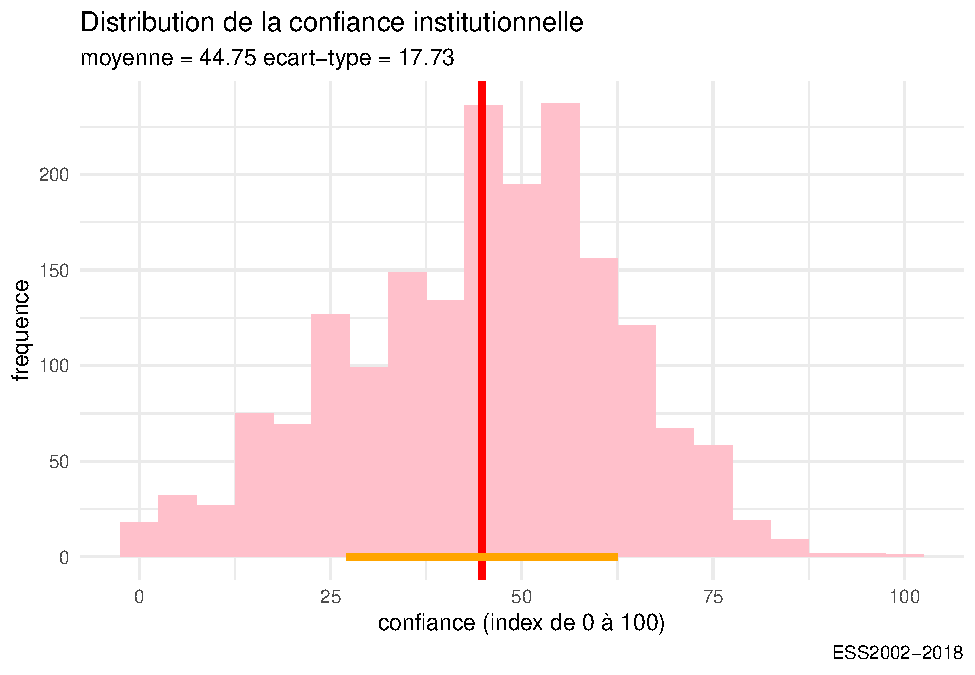
\includegraphics{bookdown-demo_files/figure-latex/303-1.pdf}

Diagramme de densité : Au lieu de représenter les effectifs, on ramène l'effectif total à 1.

\begin{Shaded}
\begin{Highlighting}[]
\NormalTok{g04<-}\KeywordTok{ggplot}\NormalTok{(foo,}\KeywordTok{aes}\NormalTok{(}\DataTypeTok{x=}\NormalTok{trust_institut))}\OperatorTok{+}\StringTok{ }
\StringTok{  }\KeywordTok{geom_density}\NormalTok{(}\DataTypeTok{fill=}\StringTok{"pink2"}\NormalTok{) }\OperatorTok{+}
\StringTok{  }\KeywordTok{labs}\NormalTok{(}\DataTypeTok{title=} \StringTok{"Fonction de densité de probabilité"}\NormalTok{, }\DataTypeTok{caption=}\StringTok{"ESS2002-2018"}\NormalTok{,}\DataTypeTok{y=} \StringTok{"frequence"}\NormalTok{,}\DataTypeTok{x=}\StringTok{"Confiance (index de 1 à 100)"}\NormalTok{) }
\NormalTok{g04}
\end{Highlighting}
\end{Shaded}

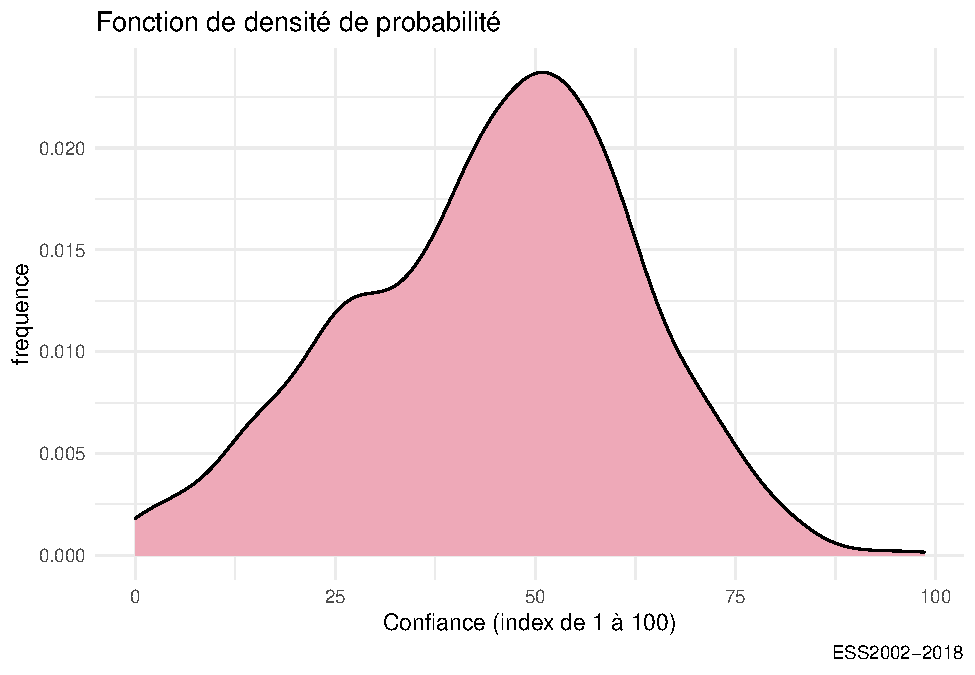
\includegraphics{bookdown-demo_files/figure-latex/304-1.pdf}

enfin on peut examiner par rapport à une distribution théorique, en l'occurrence une distribution gaussienne, ou normale, de paramètres égaux à la moyenne et la variance empirique de la distribution. L'ajustement est convenable même si on observe une déviation sur la droite. C'est pourquoi on calcule aussi la Kurtosis et le skewness de la distribution.

\begin{Shaded}
\begin{Highlighting}[]
\CommentTok{#On a déjà calculé la moyenne : mean}
\CommentTok{#il nous manque l'écart-type et }
\NormalTok{sd<-}\KeywordTok{sd}\NormalTok{(foo}\OperatorTok{$}\NormalTok{trust_institut, }\DataTypeTok{na.rm=}\OtherTok{TRUE}\NormalTok{)}
\KeywordTok{library}\NormalTok{(moments)}
\NormalTok{sk<-}\KeywordTok{skewness}\NormalTok{(foo}\OperatorTok{$}\NormalTok{trust_institut)}
\NormalTok{ks<-}\KeywordTok{kurtosis}\NormalTok{(foo}\OperatorTok{$}\NormalTok{trust_institut)}


\NormalTok{g05<-}\KeywordTok{ggplot}\NormalTok{(foo,}\KeywordTok{aes}\NormalTok{(}\DataTypeTok{x=}\NormalTok{trust_institut))}\OperatorTok{+}\StringTok{   }
\StringTok{  }\KeywordTok{labs}\NormalTok{(}\DataTypeTok{title=} \StringTok{"Distribution de la confiance institutionnelle"}\NormalTok{, }\DataTypeTok{caption=}\StringTok{"ESS2002-2018"}\NormalTok{,}\DataTypeTok{y=} \StringTok{"frequence"}\NormalTok{,}\DataTypeTok{x=}\StringTok{"confiance (index de 0 à 100)"}\NormalTok{) }\OperatorTok{+}
\StringTok{  }\KeywordTok{geom_density}\NormalTok{(}\DataTypeTok{fill=}\StringTok{"pink2"}\NormalTok{)}\OperatorTok{+}
\StringTok{  }\KeywordTok{stat_function}\NormalTok{(}\DataTypeTok{fun =}\NormalTok{ dnorm,}\DataTypeTok{color=}\StringTok{"red"}\NormalTok{,}\DataTypeTok{size=}\FloatTok{1.2}\NormalTok{, }\DataTypeTok{args =} \KeywordTok{list}\NormalTok{(}\DataTypeTok{mean =}\NormalTok{moy, }\DataTypeTok{sd=}\NormalTok{sd))}
   
\NormalTok{g05}
\end{Highlighting}
\end{Shaded}

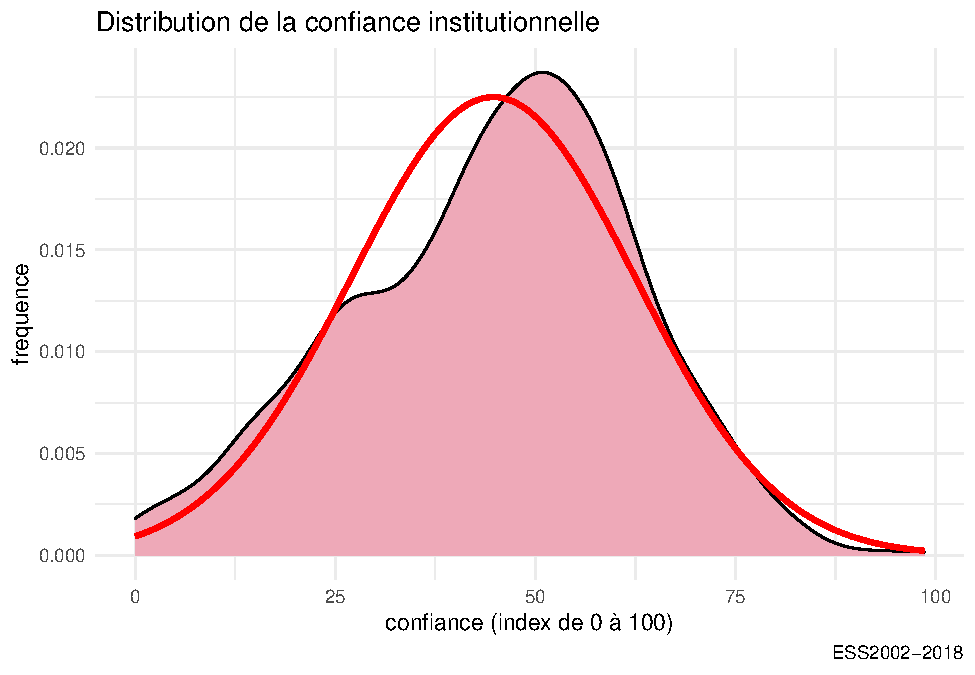
\includegraphics{bookdown-demo_files/figure-latex/305-1.pdf}

Un grand classique du test de normalité d'une distribution est le diagramme QQ

\begin{Shaded}
\begin{Highlighting}[]
\NormalTok{g06 <-}\StringTok{ }\KeywordTok{ggplot}\NormalTok{(foo, }\KeywordTok{aes}\NormalTok{(}\DataTypeTok{sample =}\NormalTok{ trust_institut)) }\OperatorTok{+}\StringTok{ }
\StringTok{  }\KeywordTok{stat_qq}\NormalTok{() }\OperatorTok{+}\StringTok{ }\KeywordTok{stat_qq_line}\NormalTok{()}\OperatorTok{+}\StringTok{ }
\StringTok{  }\KeywordTok{labs}\NormalTok{(}\DataTypeTok{title=} \StringTok{"QQplot confiance interpersonnelle"}\NormalTok{, }\DataTypeTok{caption=}\StringTok{"ESS2002-2018"}\NormalTok{,}\DataTypeTok{y=} \StringTok{"Echantillon"}\NormalTok{,}\DataTypeTok{x=}\StringTok{"Théorique"}\NormalTok{) }
\NormalTok{g06}
\end{Highlighting}
\end{Shaded}

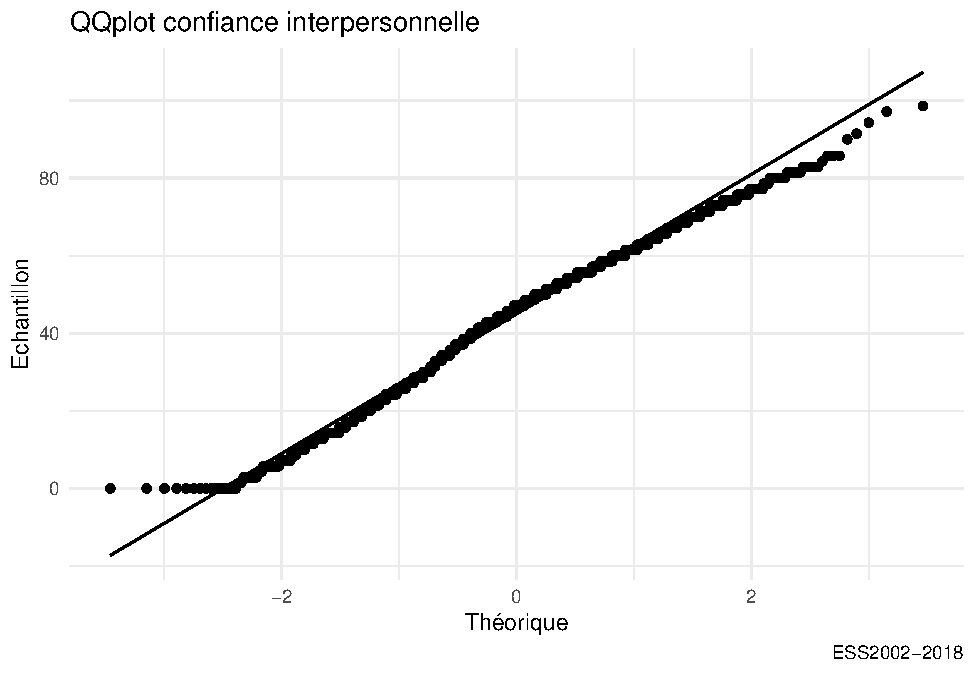
\includegraphics{bookdown-demo_files/figure-latex/306-1.pdf}

On fini cette étude détaillée par l'ajustement d'abord d'un modèle (loi normale) aux données. Ensuite d'un modèle de mélange ( Mixture model) par lequel on défiit la loi de distribution sous jascente, comme un mélange entre deux populations normale de paramètres distincts.

\url{https://tinyheero.github.io/2015/10/13/mixture-model.html}

\begin{Shaded}
\begin{Highlighting}[]
\NormalTok{df0<-df }\OperatorTok\StringTok{ }\KeywordTok{na.omit}\NormalTok{() }
\KeywordTok{library}\NormalTok{(MASS)}
\NormalTok{fit<-}\KeywordTok{fitdistr}\NormalTok{(df0}\OperatorTok{$}\NormalTok{trust_interpersonnel,}\StringTok{"normal"}\NormalTok{) }
\NormalTok{fit}
\end{Highlighting}
\end{Shaded}

\begin{verbatim}
##       mean           sd     
##   52.48548790   16.57617220 
##  ( 0.09344363) ( 0.06607462)
\end{verbatim}

\begin{Shaded}
\begin{Highlighting}[]
\NormalTok{g07<-}\StringTok{ }\NormalTok{g05}\OperatorTok{+}\KeywordTok{stat_function}\NormalTok{(}\DataTypeTok{fun =}\NormalTok{  dnorm ,}\DataTypeTok{color=}\StringTok{"orange"}\NormalTok{,}\DataTypeTok{size=}\FloatTok{1.2}\NormalTok{, }\DataTypeTok{args =} \KeywordTok{list}\NormalTok{( }\DataTypeTok{mean=}\FloatTok{52.48}\NormalTok{,  }\DataTypeTok{sd=}\FloatTok{16.57}\NormalTok{))}
\NormalTok{g07}
\end{Highlighting}
\end{Shaded}

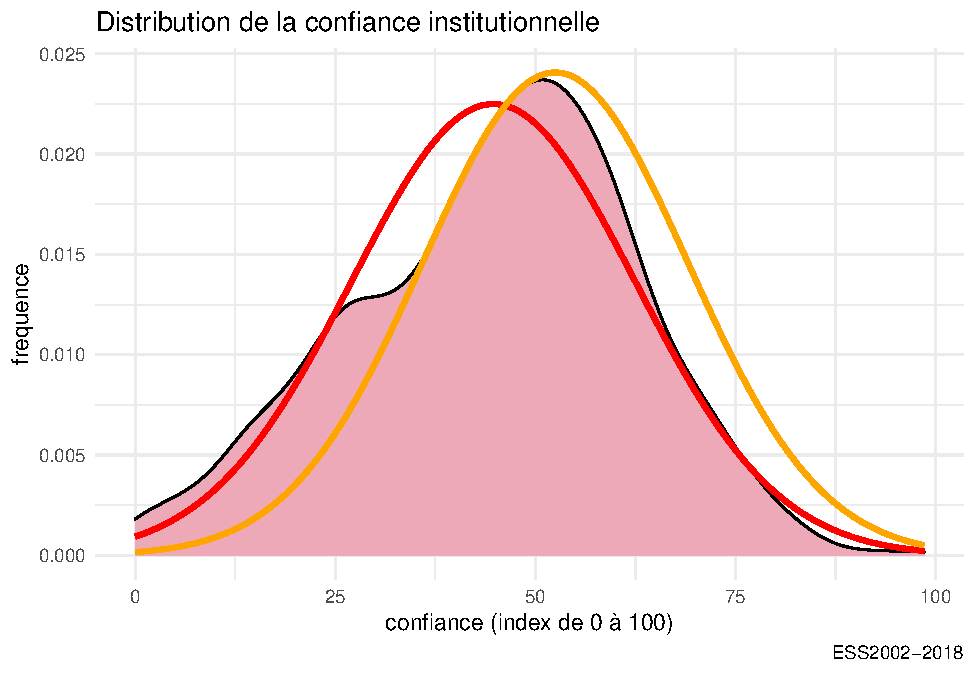
\includegraphics{bookdown-demo_files/figure-latex/307-1.pdf}

\begin{Shaded}
\begin{Highlighting}[]
\KeywordTok{library}\NormalTok{(mixtools)}
\NormalTok{trust =}\StringTok{ }\NormalTok{foo}\OperatorTok{$}\NormalTok{trust_institut}
\NormalTok{mixmdl =}\StringTok{ }\KeywordTok{normalmixEM}\NormalTok{(trust, }\DataTypeTok{k=}\DecValTok{2}\NormalTok{)}
\end{Highlighting}
\end{Shaded}

\begin{verbatim}
## number of iterations= 517
\end{verbatim}

\begin{Shaded}
\begin{Highlighting}[]
\NormalTok{mixmdl}\OperatorTok{$}\NormalTok{mu}
\end{Highlighting}
\end{Shaded}

\begin{verbatim}
## [1] 39.23077 56.04167
\end{verbatim}

\begin{Shaded}
\begin{Highlighting}[]
\NormalTok{mixmdl}\OperatorTok{$}\NormalTok{sigma}
\end{Highlighting}
\end{Shaded}

\begin{verbatim}
## [1] 17.90247 10.56090
\end{verbatim}

\begin{Shaded}
\begin{Highlighting}[]
\NormalTok{mixmdl}\OperatorTok{$}\NormalTok{lambda}
\end{Highlighting}
\end{Shaded}

\begin{verbatim}
## [1] 0.6719521 0.3280479
\end{verbatim}

\begin{Shaded}
\begin{Highlighting}[]
\KeywordTok{plot}\NormalTok{(mixmdl,}\DataTypeTok{which=}\DecValTok{2}\NormalTok{)}
\KeywordTok{lines}\NormalTok{(}\KeywordTok{density}\NormalTok{(trust), }\DataTypeTok{lty=}\DecValTok{2}\NormalTok{, }\DataTypeTok{lwd=}\DecValTok{2}\NormalTok{)}
\end{Highlighting}
\end{Shaded}

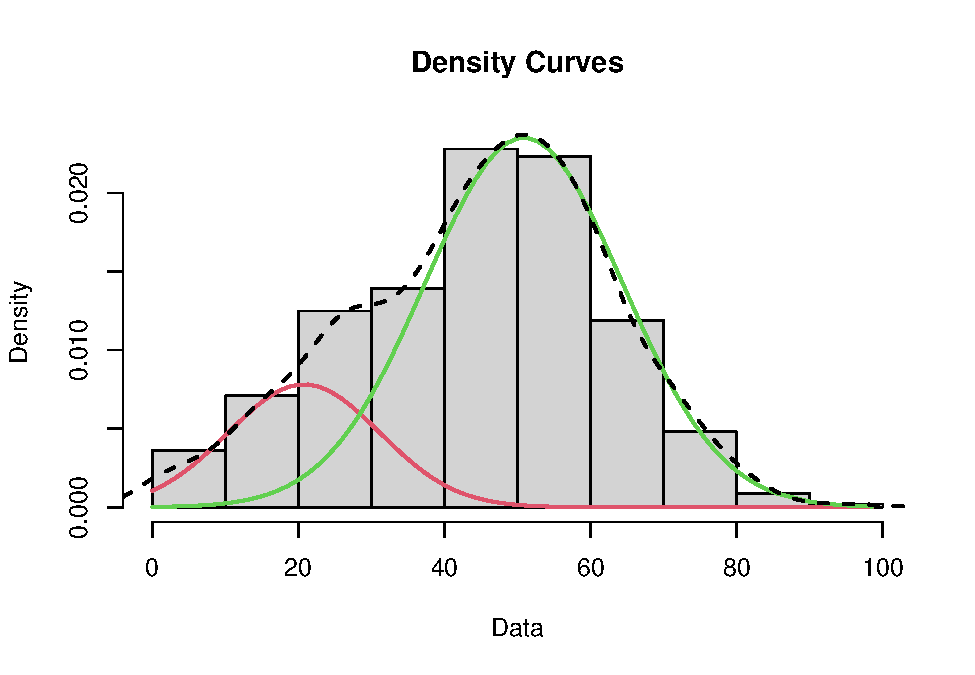
\includegraphics{bookdown-demo_files/figure-latex/307-2.pdf}

Finalement si notre distribution est univariée, car n'étudiant qu'une variable, on peut quand distinguer deux population distinctes.

\hypertarget{dautres-muxe9thodes}{%
\subsubsection{D'autres méthodes}\label{dautres-muxe9thodes}}

Il n'y a pas que l'histogram ou le diagramme de densité, d'autres méthodes sont utiles, surtout quand on veut comparer des groupes ( ce sera l'objet du prochain chapitre). Il s'agit du diagramme à moustache et du diagramme en violon.

\begin{Shaded}
\begin{Highlighting}[]
\NormalTok{g0306 <-}\StringTok{ }\KeywordTok{ggplot}\NormalTok{(foo, }\KeywordTok{aes}\NormalTok{(}\DataTypeTok{y =}\NormalTok{ trust_institut, }\DataTypeTok{x=}\DecValTok{1}\NormalTok{)) }\OperatorTok{+}\StringTok{ }
\KeywordTok{geom_boxplot}\NormalTok{(}\DataTypeTok{fill=}\StringTok{"Grey"}\NormalTok{) }

\NormalTok{g0307 <-}\StringTok{ }\KeywordTok{ggplot}\NormalTok{(foo, }\KeywordTok{aes}\NormalTok{(}\DataTypeTok{x=}\DecValTok{1}\NormalTok{,}\DataTypeTok{y =}\NormalTok{ trust_institut)) }\OperatorTok{+}\StringTok{ }
\KeywordTok{geom_violin}\NormalTok{(}\DataTypeTok{fill=}\StringTok{"Gold"}\NormalTok{) }\OperatorTok{+}\StringTok{ }\KeywordTok{labs}\NormalTok{(}\DataTypeTok{x=}\StringTok{"density"}\NormalTok{)}

\KeywordTok{plot_grid}\NormalTok{(g0306, g0307, }\DataTypeTok{labels =} \KeywordTok{c}\NormalTok{(}\StringTok{"Boxplot"}\NormalTok{,}\StringTok{"Violin plot"}\NormalTok{),}
  \DataTypeTok{label_size =} \DecValTok{12}
\NormalTok{)}
\end{Highlighting}
\end{Shaded}

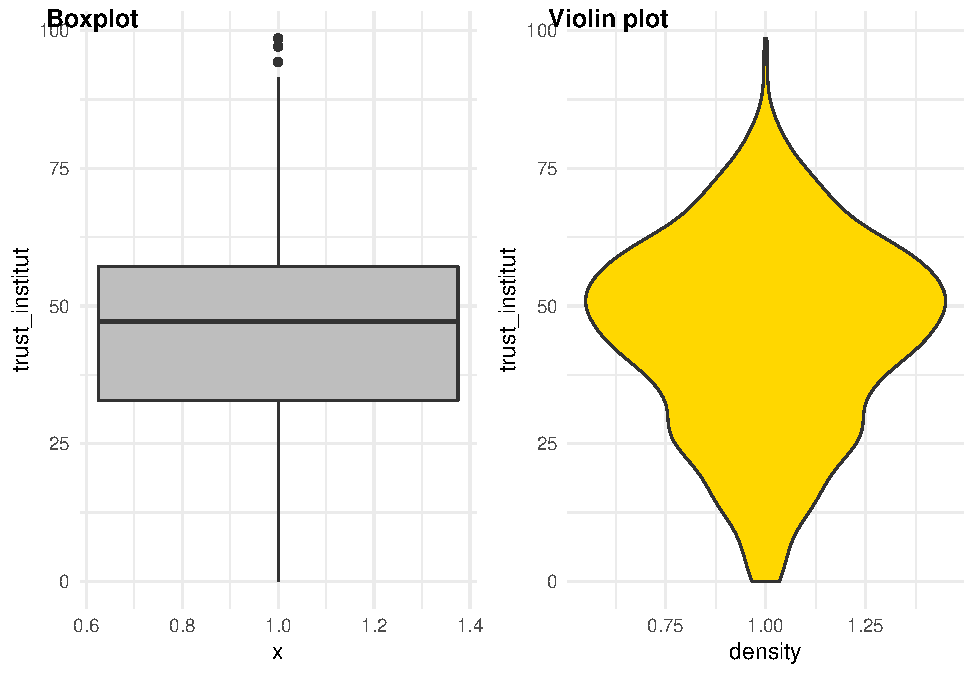
\includegraphics{bookdown-demo_files/figure-latex/308a-1.pdf}

\hypertarget{quand-la-variable-est-qualitative}{%
\subsection{Quand la variable est qualitative}\label{quand-la-variable-est-qualitative}}

Quand la variable est qualitative, que ses variables sont discrètes, la manière de représenter la plus commune est le fameux camembert que les experts écartent. Un diagramme en barre représente mieux les proportions.

Un premier exemple pour représenter les vagues d'enquêtes

\begin{Shaded}
\begin{Highlighting}[]
\NormalTok{g08<-}\KeywordTok{ggplot}\NormalTok{(df,}\KeywordTok{aes}\NormalTok{(}\DataTypeTok{x=}\NormalTok{age))}\OperatorTok{+}
\StringTok{  }\KeywordTok{geom_bar}\NormalTok{(}\DataTypeTok{fill=}\StringTok{"skyblue"}\NormalTok{)}\OperatorTok{+}
\StringTok{  }\KeywordTok{labs}\NormalTok{(}\DataTypeTok{title=} \StringTok{"Distribution par classe d'âge"}\NormalTok{, }\DataTypeTok{caption=}\StringTok{"ESS2002-2018"}\NormalTok{,}\DataTypeTok{y=} \StringTok{"frequence"}\NormalTok{,}\DataTypeTok{x=}\StringTok{"Vague d'enquête") }
\StringTok{g08}
\end{Highlighting}
\end{Shaded}

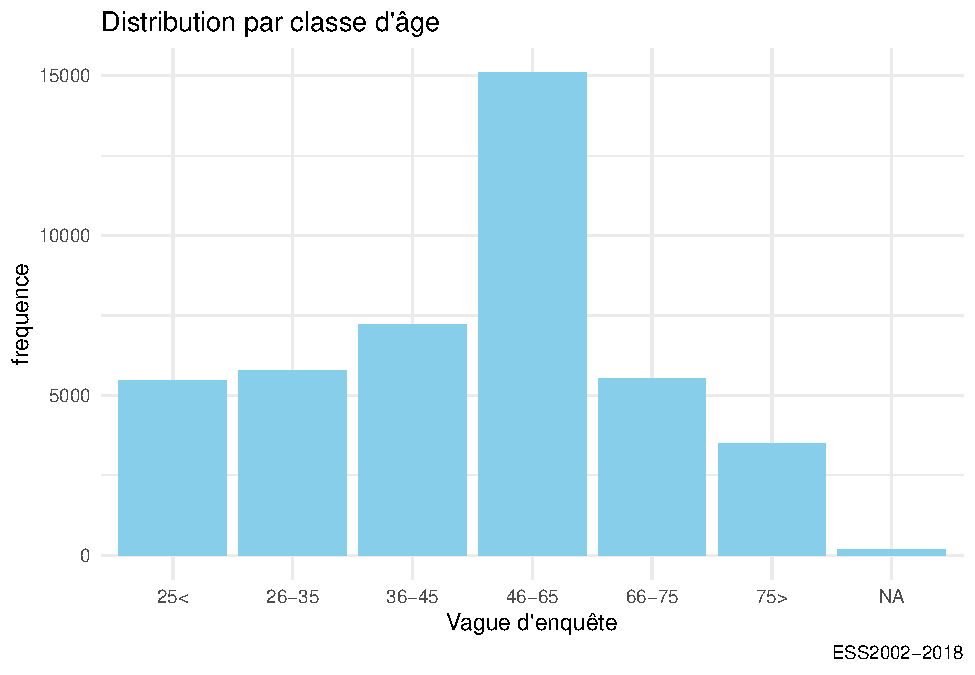
\includegraphics{bookdown-demo_files/figure-latex/308-1.pdf}

Avec quelques améliorations : contôle de la couleurs des barres, ajout des \% et pivot pour une meilleure lecture.

\begin{Shaded}
\begin{Highlighting}[]
\NormalTok{foo<-df }\OperatorTok
\StringTok{  }\KeywordTok{filter}\NormalTok{(}\OperatorTok{!}\KeywordTok{is.na}\NormalTok{(age))}

\NormalTok{g10<-}\KeywordTok{ggplot}\NormalTok{(foo,}\KeywordTok{aes}\NormalTok{(}\DataTypeTok{x=}\NormalTok{age, }\DataTypeTok{y =} \KeywordTok{prop.table}\NormalTok{(}\KeywordTok{stat}\NormalTok{(count)),}\DataTypeTok{label =}\NormalTok{ scales}\OperatorTok{::}\KeywordTok{percent}\NormalTok{(}\KeywordTok{prop.table}\NormalTok{(}\KeywordTok{stat}\NormalTok{(count)))))}\OperatorTok{+}
\StringTok{  }\KeywordTok{geom_bar}\NormalTok{(}\KeywordTok{aes}\NormalTok{(}\DataTypeTok{fill =}\NormalTok{ age)) }\OperatorTok{+}\StringTok{  }
\StringTok{  }\KeywordTok{coord_flip}\NormalTok{()}\OperatorTok{+}\StringTok{ }
\StringTok{  }\KeywordTok{labs}\NormalTok{(}\DataTypeTok{title=} \StringTok{"Répartition de la population par classe d'âge"}\NormalTok{, }\DataTypeTok{caption=}\StringTok{"ESS2002-2018"}\NormalTok{,}\DataTypeTok{y=} \StringTok{"%"}\NormalTok{,}\DataTypeTok{x=}\StringTok{"classes d'age"}\NormalTok{) }\OperatorTok{+}
\StringTok{  }\KeywordTok{scale_y_continuous}\NormalTok{(}\DataTypeTok{labels =}\NormalTok{ scales}\OperatorTok{::}\NormalTok{percent)}\OperatorTok{+}\StringTok{ }\CommentTok{#contrôle de l'échelle des % et du format}
\StringTok{  }\KeywordTok{scale_fill_brewer}\NormalTok{()}\OperatorTok{+}
\StringTok{  }\KeywordTok{geom_text}\NormalTok{(}\DataTypeTok{stat =} \StringTok{'count'}\NormalTok{,}\DataTypeTok{position =} \KeywordTok{position_dodge}\NormalTok{(.}\DecValTok{9}\NormalTok{),  }\DataTypeTok{hjust =} \DecValTok{1}\NormalTok{, }\DataTypeTok{size =} \DecValTok{3}\NormalTok{)}


\NormalTok{g10}
\end{Highlighting}
\end{Shaded}

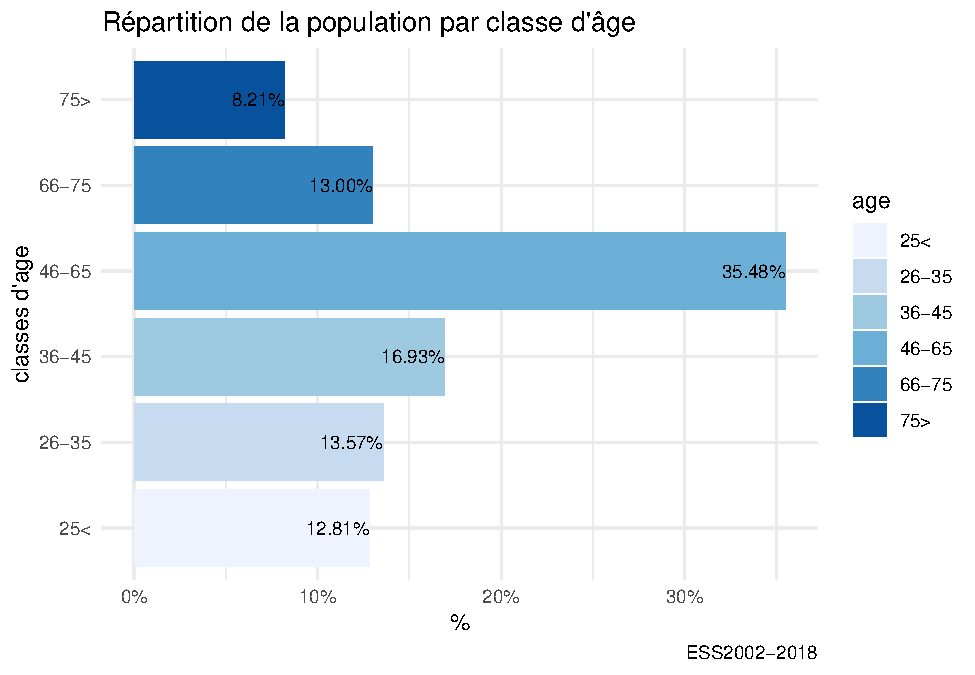
\includegraphics{bookdown-demo_files/figure-latex/309-1.pdf}

si on tient au diagramme en secteur

\begin{Shaded}
\begin{Highlighting}[]
\NormalTok{foo<-df }\OperatorTok\KeywordTok{filter}\NormalTok{(}\OperatorTok{!}\KeywordTok{is.na}\NormalTok{(age))}
\NormalTok{g10<-}\KeywordTok{ggplot}\NormalTok{(foo,}\KeywordTok{aes}\NormalTok{(}\DataTypeTok{x=}\StringTok{""}\NormalTok{, }\DataTypeTok{y =} \KeywordTok{prop.table}\NormalTok{(}\KeywordTok{stat}\NormalTok{(count)),}\DataTypeTok{label =}\NormalTok{ scales}\OperatorTok{::}\KeywordTok{percent}\NormalTok{(}\KeywordTok{prop.table}\NormalTok{(}\KeywordTok{stat}\NormalTok{(count)))))}\OperatorTok{+}
\StringTok{  }\KeywordTok{geom_bar}\NormalTok{(}\KeywordTok{aes}\NormalTok{(}\DataTypeTok{fill =}\NormalTok{ age)) }\OperatorTok{+}\StringTok{  }
\StringTok{  }\KeywordTok{labs}\NormalTok{(}\DataTypeTok{title=} \StringTok{"Répartition de la population par classe d'âge"}\NormalTok{, }\DataTypeTok{caption=}\StringTok{"ESS2002-2018"}\NormalTok{,}\DataTypeTok{y=} \StringTok{"%"}\NormalTok{,}\DataTypeTok{x=}\StringTok{"classes d'age"}\NormalTok{) }\OperatorTok{+}
\StringTok{  }\KeywordTok{geom_text}\NormalTok{(}\DataTypeTok{stat =} \StringTok{'count'}\NormalTok{,}\DataTypeTok{position =} \KeywordTok{position_dodge}\NormalTok{(.}\DecValTok{9}\NormalTok{),  }\DataTypeTok{hjust =} \DecValTok{1}\NormalTok{, }\DataTypeTok{size =} \DecValTok{3}\NormalTok{) }\OperatorTok{+}\StringTok{ }
\StringTok{  }\KeywordTok{coord_polar}\NormalTok{(}\StringTok{"y"}\NormalTok{, }\DataTypeTok{start=}\DecValTok{0}\NormalTok{)}



\NormalTok{g10}
\end{Highlighting}
\end{Shaded}

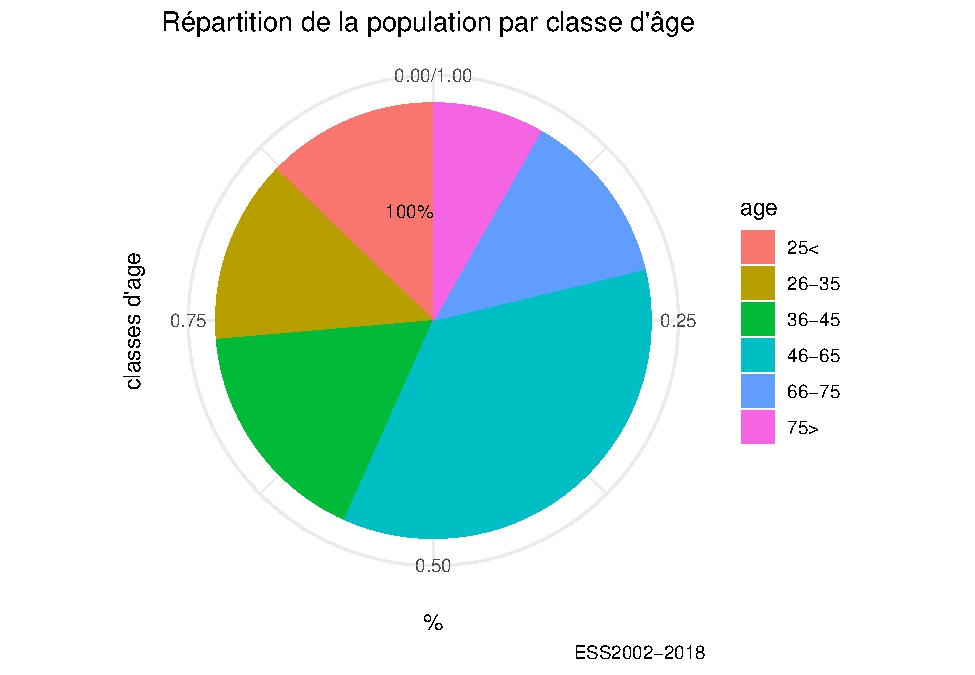
\includegraphics{bookdown-demo_files/figure-latex/310-1.pdf}
\url{https://cran.r-project.org/web/packages/treemapify/vignettes/introduction-to-treemapify.html}

si on tient au diagramme en cercle, autant opter pour un treemap avec la bibliothèque treemapifi

\begin{Shaded}
\begin{Highlighting}[]
\KeywordTok{library}\NormalTok{(treemapify)}
\NormalTok{tree1<-df }\OperatorTok\StringTok{ }
\StringTok{  }\KeywordTok{mutate}\NormalTok{(}\DataTypeTok{n=}\DecValTok{1}\NormalTok{)}\OperatorTok\KeywordTok{group_by}\NormalTok{(age) }\OperatorTok\StringTok{ }
\StringTok{  }\KeywordTok{summarize}\NormalTok{(}\DataTypeTok{n=}\KeywordTok{sum}\NormalTok{(n)) }\OperatorTok
\StringTok{  }\KeywordTok{filter}\NormalTok{(}\OperatorTok{!}\KeywordTok{is.na}\NormalTok{(age))}

\NormalTok{g11 <-}\StringTok{ }\KeywordTok{ggplot}\NormalTok{(tree1, }\KeywordTok{aes}\NormalTok{(}\DataTypeTok{area =}\NormalTok{ n, }\DataTypeTok{fill=}\NormalTok{n),}\DataTypeTok{label=}\NormalTok{age) }\OperatorTok{+}
\StringTok{  }\KeywordTok{geom_treemap}\NormalTok{() }\OperatorTok{+}
\StringTok{  }\KeywordTok{geom_treemap_text}\NormalTok{(}\KeywordTok{aes}\NormalTok{(}\DataTypeTok{label=}\NormalTok{age),}\DataTypeTok{colour =} \StringTok{"white"}\NormalTok{, }\DataTypeTok{place =} \StringTok{"centre"}\NormalTok{,}\DataTypeTok{grow =} \OtherTok{FALSE}\NormalTok{)}\OperatorTok{+}
\StringTok{  }\KeywordTok{labs}\NormalTok{(}\DataTypeTok{title=} \StringTok{"Répartition de la population par classe d'âge"}\NormalTok{, }\DataTypeTok{caption=}\StringTok{"ESS2002-2018"}\NormalTok{,}\DataTypeTok{y=} \OtherTok{NULL}\NormalTok{,}\DataTypeTok{x=}\OtherTok{NULL}\NormalTok{) }

\NormalTok{g11}
\end{Highlighting}
\end{Shaded}

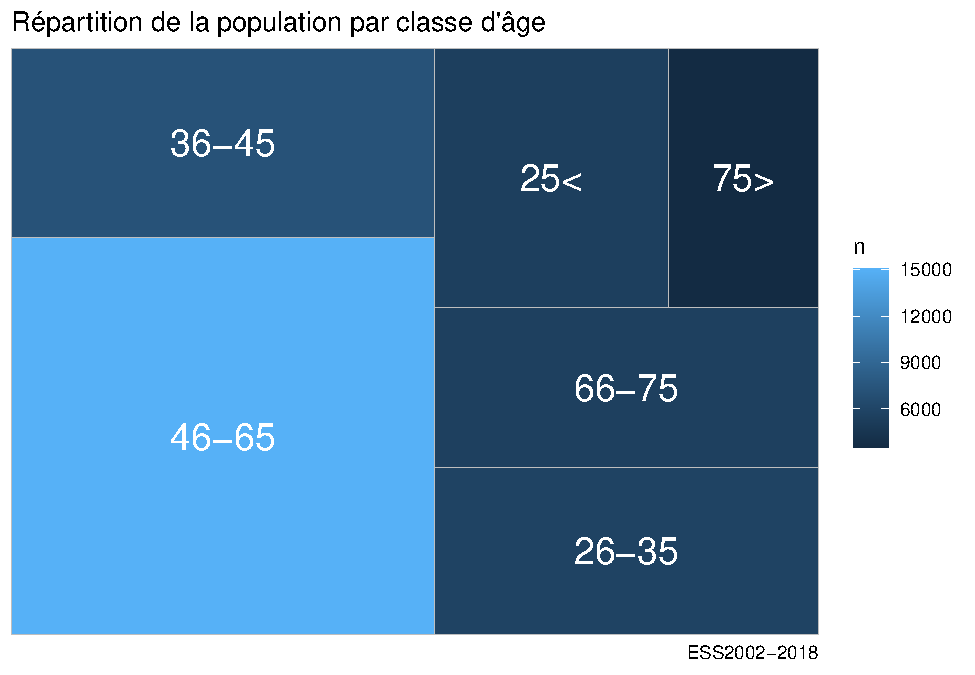
\includegraphics{bookdown-demo_files/figure-latex/311-1.pdf}

\hypertarget{analyse-bi-variuxe9e}{%
\chapter{Analyse bi variée}\label{analyse-bi-variuxe9e}}

Comme son nom l'indique, il s'agit d'examiner la relation entre deux variables et d'étudier leur distribution conjointe. On distinguera 3 situations et on examinera pour chaune les modes de représentations graphiques ainsi que les tests associés qui permette de s'assurer que la relation apparente est effective.

\begin{enumerate}
\def\labelenumi{\alph{enumi})}
\item
  Deux variables quantitatives : scatterplot et corélations
\item
  deux variable qualitatives : tableau croisé et test du chi2
\item
  une variable quanti et une variable quali. Compariaons de moyennes et ANOVA
\item
  par comparer des distribution de plusieurs groupes (variables catégorielles)
\item
  par comparer des moyennes d'une variable dépendante en fonction de plusieurs variables indépendantes catégorielle
\item
  mesurer l'association entre deux variables qualitatives
\end{enumerate}

\hypertarget{diagrammes-xy---la-magie-des-corruxe9lations}{%
\section{Diagrammes xy - la magie des corrélations}\label{diagrammes-xy---la-magie-des-corruxe9lations}}

Venons en à analyser les relations entre deux variables quantitatives.

\begin{Shaded}
\begin{Highlighting}[]
\NormalTok{foo<-df }\OperatorTok
\StringTok{  }\KeywordTok{filter}\NormalTok{(cntry}\OperatorTok{==}\StringTok{"FR"} \OperatorTok{&}\StringTok{ }\NormalTok{Year}\OperatorTok{==}\StringTok{"2018"}\NormalTok{) }\CommentTok{#selection de l'echantillon}

\NormalTok{g31<-}\StringTok{ }\KeywordTok{ggplot}\NormalTok{(foo, }\KeywordTok{aes}\NormalTok{(}\DataTypeTok{x=}\NormalTok{ trust_interpersonnel,}\DataTypeTok{y=}\NormalTok{trust_institut)) }\OperatorTok{+}
\StringTok{  }\KeywordTok{geom_point}\NormalTok{( }\DataTypeTok{size=}\FloatTok{0.1}\NormalTok{)}
     
\NormalTok{g31}
\end{Highlighting}
\end{Shaded}

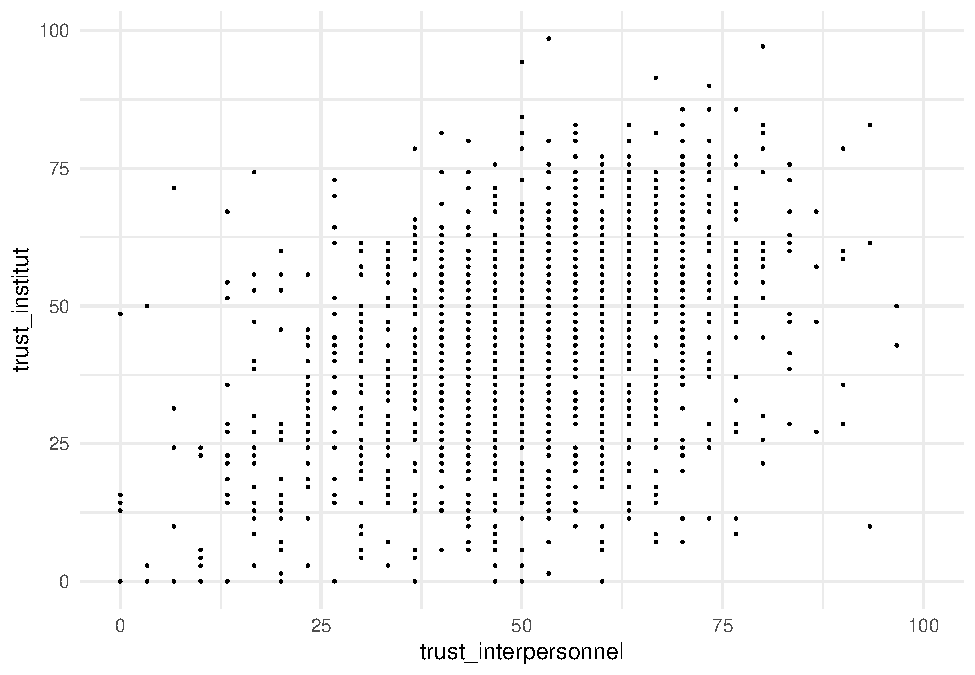
\includegraphics{bookdown-demo_files/figure-latex/412-1.pdf}

Ce graphe est peu clair, il y a trop de points qui prennent des valeurs discrètes. Une astuce est de donner une position aléatoire pour sur disperser, on fait mieux apparaitre la densité de points. On ajoute la représentation de deux courbe d'ajustement, l'une linéraire et l'autre non linéaires.

Mais en attendant en voici un calcul élémentaire.

le calcul de la variance

\[{SS}_{xx} = \sum (x - \bar{x})^2 = \sum x^2 - \frac {(\sum x)^2}{n}\]
le calcul de la covariance

\[{SS}_{xy} = \sum (x - \bar{x})(y - \bar{y}) = \sum xy - \frac {(\sum x)(\sum y)}{n}\]
et la corrélation qui est le rapport de la covariance sur la racine carrée du produit des variances de x et y.

\[r = \frac {{SS}_{xy}}{\sqrt {{SS}_{xx}{SS}_{yy}}}\]

La corrélation est de l'ordre d'un peu plus de 0,40 ce qui est assez élevé mais laisse une certaine indépendance des variables. Elle désignent des objets liés mais distinct. On peut tester l'hypothèse qu'en réalité cette corrélation est nulle. Le test conduit au rejet de l'hypothèse nulle de manière très nette, compte-tenu de l'échantillon l'intervalle de confiance est compris entre 0.36 et 0.44.

\begin{Shaded}
\begin{Highlighting}[]
\CommentTok{#psych}
\NormalTok{r<-}\KeywordTok{cor.test}\NormalTok{(foo}\OperatorTok{$}\NormalTok{trust_interpersonnel, foo}\OperatorTok{$}\NormalTok{trust_institut) }\CommentTok{#le test vient du package psych}
\NormalTok{r}
\end{Highlighting}
\end{Shaded}

\begin{verbatim}
## 
##  Pearson's product-moment correlation
## 
## data:  foo$trust_interpersonnel and foo$trust_institut
## t = 18.861, df = 1821, p-value < 2.2e-16
## alternative hypothesis: true correlation is not equal to 0
## 95 percent confidence interval:
##  0.3651235 0.4419644
## sample estimates:
##      cor 
## 0.404257
\end{verbatim}

\begin{Shaded}
\begin{Highlighting}[]
\NormalTok{rp<-}\KeywordTok{round}\NormalTok{(r}\OperatorTok{$}\NormalTok{estimate,}\DecValTok{3}\NormalTok{)}
\NormalTok{rp}
\end{Highlighting}
\end{Shaded}

\begin{verbatim}
##   cor 
## 0.404
\end{verbatim}

Améliorons le graphe On peut souhaiter ajouter une droite des moindre carrés (calculée pour chaque vague d'enquête pour évaluer la stabilité de la relation dans le temps). Les lignes sont parallèles, la corrélation ne change pas dans le temps, c'est une relation stable. Les deux formes de confiance vont dans le meme sens. On verra dans un autre chapitre comment calculer ces droites de corrélations.

\begin{Shaded}
\begin{Highlighting}[]
\KeywordTok{library}\NormalTok{(ggExtra)}
\NormalTok{g32<-}\KeywordTok{ggplot}\NormalTok{(foo, }\KeywordTok{aes}\NormalTok{(}\DataTypeTok{x=}\NormalTok{ trust_interpersonnel,}\DataTypeTok{y=}\NormalTok{trust_institut)) }\OperatorTok{+}
\StringTok{  }\KeywordTok{geom_point}\NormalTok{(}\DataTypeTok{position =} \StringTok{"jitter"}\NormalTok{, }\DataTypeTok{size=}\FloatTok{0.1}\NormalTok{, }\DataTypeTok{color=}\StringTok{"grey"}\NormalTok{)}\OperatorTok{+}
\StringTok{  }\KeywordTok{geom_smooth}\NormalTok{(}\DataTypeTok{method=}\StringTok{"lm"}\NormalTok{, }\DataTypeTok{se=}\OtherTok{TRUE}\NormalTok{) }\OperatorTok{+}
\StringTok{  }\KeywordTok{geom_smooth}\NormalTok{(}\DataTypeTok{method=}\StringTok{"gam"}\NormalTok{,}\DataTypeTok{color=}\StringTok{"red"}\NormalTok{)     }\OperatorTok{+}
\StringTok{  }\KeywordTok{labs}\NormalTok{(}\DataTypeTok{title =} \StringTok{"Relation entre confiance }\CharTok{\textbackslash{}n}\StringTok{institutionnelle et interpersonnelle"}\NormalTok{, }
       \DataTypeTok{subtitle =} \KeywordTok{paste}\NormalTok{(}\StringTok{"r de pearson: "}\NormalTok{,rp ),}
       \DataTypeTok{x=} \StringTok{"Confiance interpersonnelle"}\NormalTok{,}
       \DataTypeTok{y=}\StringTok{" Confiance institutionnelle"}\NormalTok{)}

\KeywordTok{ggMarginal}\NormalTok{(g32  ,}\DataTypeTok{type =} \StringTok{"density"}\NormalTok{, }\DataTypeTok{fill =} \StringTok{"Royalblue1"}\NormalTok{, }\DataTypeTok{alpha=}\NormalTok{.}\DecValTok{5}\NormalTok{)}
\end{Highlighting}
\end{Shaded}

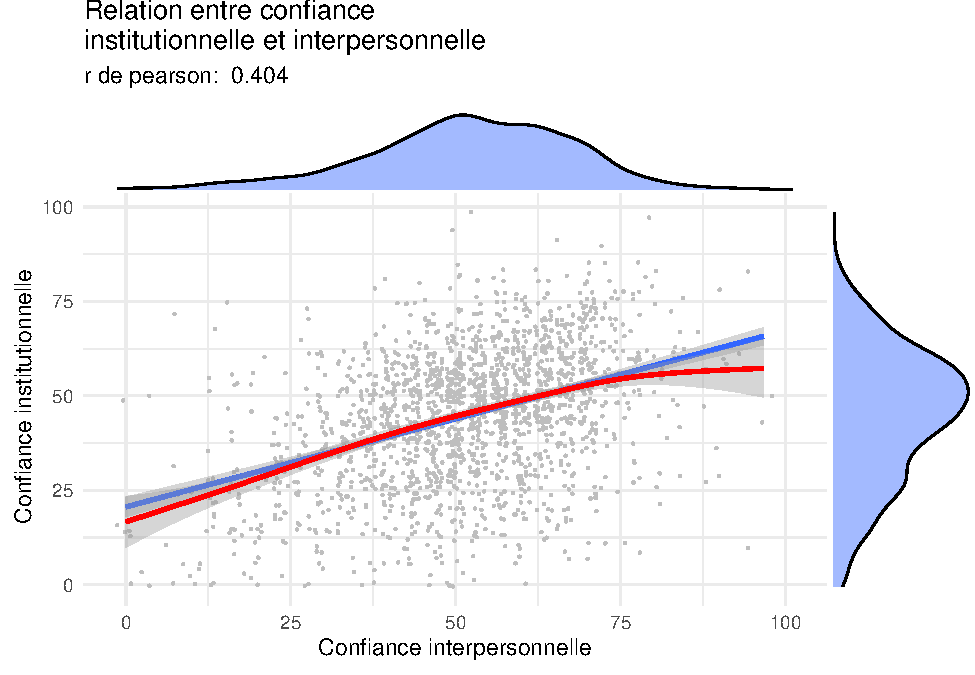
\includegraphics{bookdown-demo_files/figure-latex/415-1.pdf}

Une autre façon de représenter est celle de carte de densité de probabilité.

\begin{Shaded}
\begin{Highlighting}[]
\NormalTok{g32<-}\KeywordTok{ggplot}\NormalTok{(foo, }\KeywordTok{aes}\NormalTok{(}\DataTypeTok{x=}\NormalTok{ trust_interpersonnel,}\DataTypeTok{y=}\NormalTok{trust_institut)) }\OperatorTok{+}
\StringTok{  }\KeywordTok{geom_point}\NormalTok{(}\DataTypeTok{position =} \StringTok{"jitter"}\NormalTok{, }\DataTypeTok{size=}\FloatTok{0.1}\NormalTok{, }\DataTypeTok{color=}\StringTok{"grey"}\NormalTok{)}\OperatorTok{+}\KeywordTok{geom_density2d}\NormalTok{()}\OperatorTok{+}
\StringTok{  }\KeywordTok{labs}\NormalTok{(}\DataTypeTok{title =} \StringTok{"Relation entre confiance institutionnelle et interpersonnelles"}\NormalTok{, }\DataTypeTok{subtitle =} \KeywordTok{paste}\NormalTok{(}\StringTok{"r de pearson: "}\NormalTok{,rp ))}
  
\NormalTok{g33<-}\KeywordTok{ggplot}\NormalTok{(foo, }\KeywordTok{aes}\NormalTok{(}\DataTypeTok{x=}\NormalTok{ trust_interpersonnel,}\DataTypeTok{y=}\NormalTok{trust_institut)) }\OperatorTok{+}
\StringTok{  }\KeywordTok{geom_density2d_filled}\NormalTok{(}\KeywordTok{aes}\NormalTok{(}\DataTypeTok{fill =}\NormalTok{ ..level.., }\DataTypeTok{color =}\NormalTok{ ..level..),}
    \DataTypeTok{contour_var =} \StringTok{"density"}\NormalTok{)}\OperatorTok{+}
\StringTok{  }\KeywordTok{labs}\NormalTok{(}\DataTypeTok{title =} \StringTok{"Relation entre confiance institutionnelle et interpersonnelles"}\NormalTok{, }\DataTypeTok{subtitle =} \KeywordTok{paste}\NormalTok{(}\StringTok{"r de pearson: "}\NormalTok{,rp ))}\OperatorTok{+}\KeywordTok{theme}\NormalTok{(}\DataTypeTok{legend.position =} \StringTok{"none"}\NormalTok{)}
  

\KeywordTok{plot_grid}\NormalTok{(g32, g33, }\DataTypeTok{labels =} \KeywordTok{c}\NormalTok{(}\StringTok{'A'}\NormalTok{, }\StringTok{'B'}\NormalTok{), }\DataTypeTok{label_size =} \DecValTok{12}\NormalTok{)}
\end{Highlighting}
\end{Shaded}

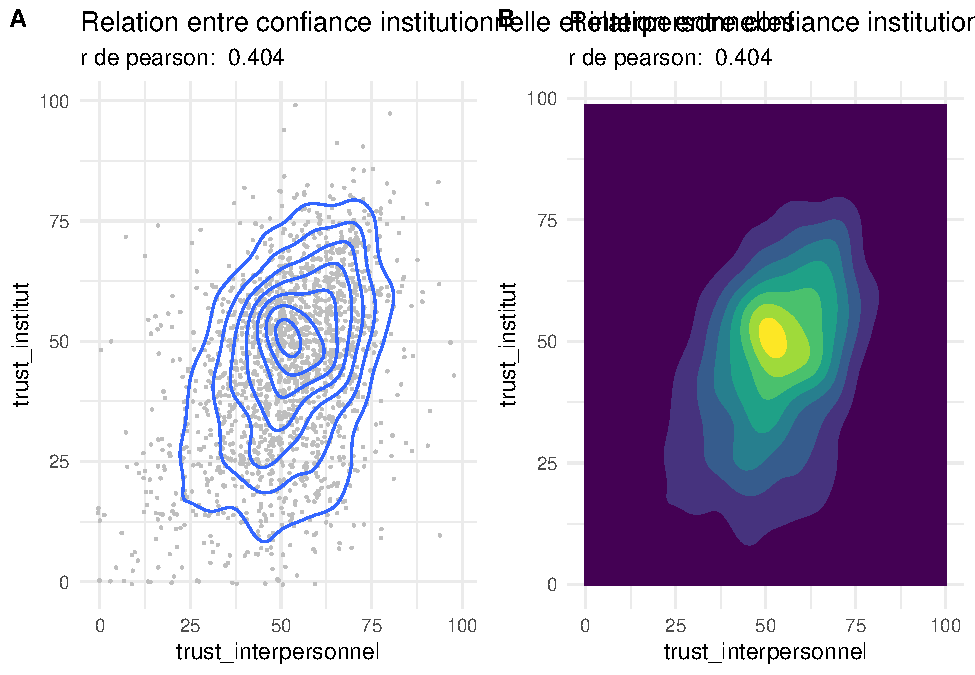
\includegraphics{bookdown-demo_files/figure-latex/416-1.pdf}

\hypertarget{comparer-les-distributions-et-des-moyennes}{%
\section{Comparer les distributions et des moyennes}\label{comparer-les-distributions-et-des-moyennes}}

Dans notre base on a pris les données de l'Allemagne et de la France. On va comparer leur distribution. Et tant qu'à faire, puisque qu'on a deux variables, on va faire deux comparaisons : par pays et par type de confiance.

A cette fin, nous construisons un tableau de données spécifique.

\begin{Shaded}
\begin{Highlighting}[]
\CommentTok{#on recode en facteur la variable}

\NormalTok{foo <-}\StringTok{ }\NormalTok{df }\OperatorTok\StringTok{ }
\StringTok{  }\NormalTok{dplyr}\OperatorTok{::}\KeywordTok{select}\NormalTok{(cntry,trust_institut, Year,trust_interpersonnel) }\OperatorTok
\StringTok{  }\KeywordTok{filter}\NormalTok{( Year}\OperatorTok{==}\StringTok{"2018"}\NormalTok{) }\OperatorTok\StringTok{ }
\StringTok{ }\NormalTok{dplyr}\OperatorTok{::}\KeywordTok{select}\NormalTok{(}\OperatorTok{-}\NormalTok{Year)}\OperatorTok
\StringTok{ }\KeywordTok{drop_na}\NormalTok{() }\OperatorTok
\StringTok{  }\KeywordTok{gather}\NormalTok{(variable, value, }\OperatorTok{-}\NormalTok{cntry) }\CommentTok{#attention plutôt utiliser pivot_longer}

\KeywordTok{head}\NormalTok{(foo)}
\end{Highlighting}
\end{Shaded}

\begin{verbatim}
## # A tibble: 6 x 3
##   cntry        variable       value
##   <chr+lbl>    <chr>          <dbl>
## 1 DE [Germany] trust_institut  58.6
## 2 DE [Germany] trust_institut  65.7
## 3 DE [Germany] trust_institut  58.6
## 4 DE [Germany] trust_institut  65.7
## 5 DE [Germany] trust_institut  48.6
## 6 DE [Germany] trust_institut  37.1
\end{verbatim}

Pour la représentation, en plus de la représentation en terme de densité, on va choisir une méthode de violon et de boxplot. On utilise une couche de ``facetting'' pour éclater ainsi la distribution des deux variables selon un critère de pays.

\begin{Shaded}
\begin{Highlighting}[]
\CommentTok{#on peut utiliser "facet"}
\NormalTok{g20<-}\KeywordTok{ggplot}\NormalTok{(foo,}\KeywordTok{aes}\NormalTok{(}\DataTypeTok{x=}\NormalTok{value))}\OperatorTok{+}\StringTok{ }\KeywordTok{geom_density}\NormalTok{(}\DataTypeTok{binwidth=}\DecValTok{10}\NormalTok{, }\DataTypeTok{fill=}\StringTok{"pink"}\NormalTok{)}\OperatorTok{+}\StringTok{ }\KeywordTok{facet_grid}\NormalTok{(cntry}\OperatorTok{~}\NormalTok{variable)}\OperatorTok{+}\StringTok{   }
\StringTok{  }\KeywordTok{labs}\NormalTok{(}\DataTypeTok{title=} \StringTok{"Confiance institutionnnelle"}\NormalTok{, }\DataTypeTok{caption=}\StringTok{"ESS2002-2018"}\NormalTok{,}\DataTypeTok{y=} \StringTok{"frequence"}\NormalTok{,}\DataTypeTok{x=}\StringTok{"Confiance"}\NormalTok{)}
\NormalTok{g20}
\end{Highlighting}
\end{Shaded}

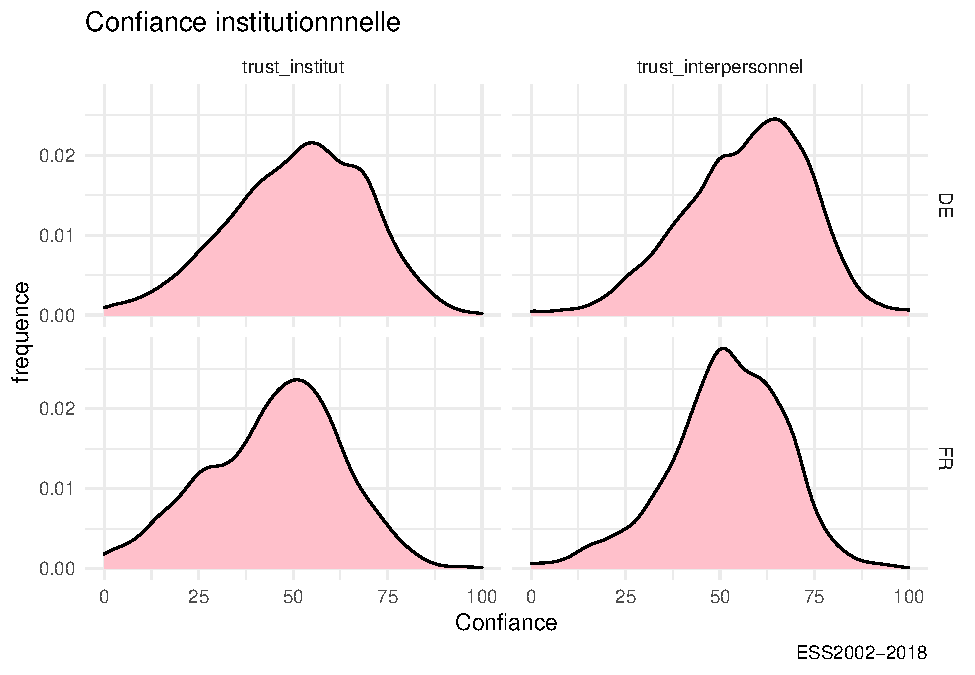
\includegraphics{bookdown-demo_files/figure-latex/418-1.pdf}

\begin{Shaded}
\begin{Highlighting}[]
\NormalTok{g21<-}\KeywordTok{ggplot}\NormalTok{(foo,}\KeywordTok{aes}\NormalTok{(}\DataTypeTok{x=}\NormalTok{variable, }\DataTypeTok{y=}\NormalTok{value))}\OperatorTok{+}\StringTok{ }
\StringTok{  }\KeywordTok{geom_violin}\NormalTok{( }\DataTypeTok{fill=}\StringTok{"pink"}\NormalTok{) }\OperatorTok{+}\StringTok{ }
\StringTok{  }\KeywordTok{geom_boxplot}\NormalTok{(}\DataTypeTok{width=}\FloatTok{0.1}\NormalTok{)}\OperatorTok{+}
\StringTok{  }\KeywordTok{facet_grid}\NormalTok{(cntry}\OperatorTok{~}\NormalTok{.)}\OperatorTok{+}\StringTok{   }
\StringTok{  }\KeywordTok{labs}\NormalTok{(}\DataTypeTok{title=} \StringTok{"Confiance institutionnnelle"}\NormalTok{, }\DataTypeTok{caption=}\StringTok{"ESS2002-2018"}\NormalTok{,}\DataTypeTok{y=} \StringTok{"frequence"}\NormalTok{,}\DataTypeTok{x=}\StringTok{"Confiance"}\NormalTok{)}
\NormalTok{g21}
\end{Highlighting}
\end{Shaded}

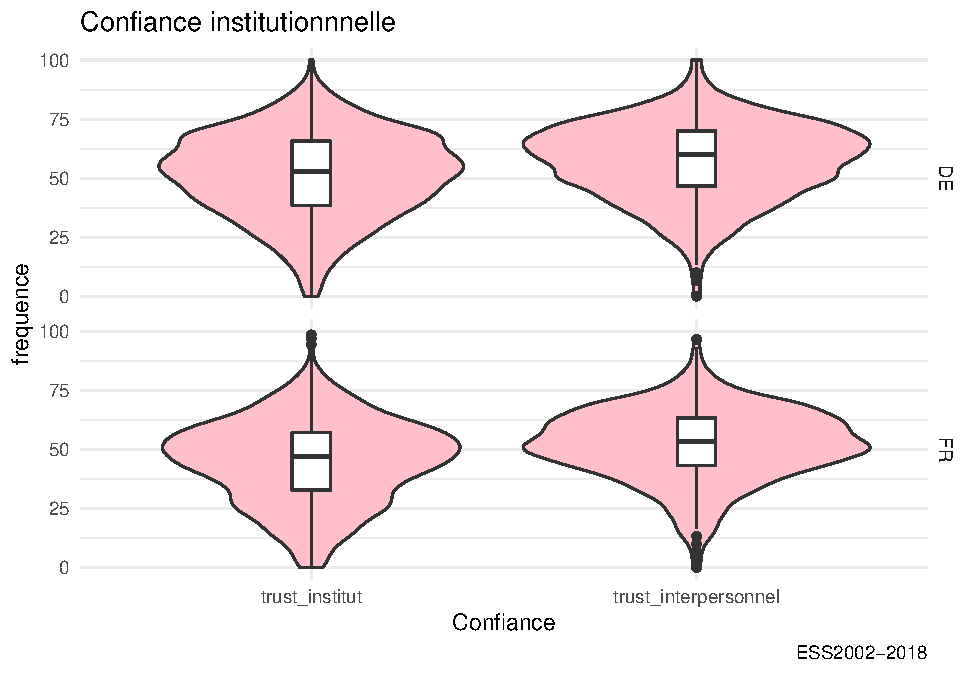
\includegraphics{bookdown-demo_files/figure-latex/418-2.pdf}

\hypertarget{comparaison-de-moyennes}{%
\subsection{Comparaison de moyennes}\label{comparaison-de-moyennes}}

Comparer des distributions est une étape initiale nécesséaire, mais en général on sera plutôt intéresser de comparer des moyennes. Par exemple, on souhaiterais savoir si les degrés de confiances institutionnnelle et interpersonnelles varient en France selon les situations de revenu.

Calculons d'abord ces moyennes avec la fonction group\_by et summarise.

\begin{Shaded}
\begin{Highlighting}[]
\NormalTok{df_wave<-df }\OperatorTok\StringTok{ }\KeywordTok{filter}\NormalTok{(cntry}\OperatorTok{==}\StringTok{"FR"} \OperatorTok{&}\StringTok{ }\NormalTok{Year}\OperatorTok{==}\StringTok{"2018"}\NormalTok{) }\OperatorTok
\StringTok{  }\KeywordTok{group_by}\NormalTok{(revenu) }\OperatorTok\StringTok{ }
\StringTok{  }\KeywordTok{summarise}\NormalTok{(}\DataTypeTok{trust_interpersonnel=}\KeywordTok{mean}\NormalTok{(trust_interpersonnel, }\DataTypeTok{na.rm=}\OtherTok{TRUE}\NormalTok{),}
            \DataTypeTok{trust_institut =}\KeywordTok{mean}\NormalTok{(trust_institut, }\DataTypeTok{na.rm=}\OtherTok{TRUE}\NormalTok{)) }\OperatorTok
\StringTok{  }\KeywordTok{filter}\NormalTok{(}\OperatorTok{!}\KeywordTok{is.na}\NormalTok{(revenu)) }\OperatorTok\StringTok{                                              }\CommentTok{#filtrer les valeurs manquantes}
\StringTok{  }\KeywordTok{gather}\NormalTok{(variable, value, }\OperatorTok{-}\NormalTok{revenu)                                        }\CommentTok{#fichier long ( pivot longer is better)}
\KeywordTok{head}\NormalTok{(df_wave)}
\end{Highlighting}
\end{Shaded}

\begin{verbatim}
## # A tibble: 6 x 3
##   revenu                        variable             value
##   <fct>                         <chr>                <dbl>
## 1 Vie confortable               trust_interpersonnel  55.6
## 2 Se débrouille avec son revenu trust_interpersonnel  51.7
## 3 Revenu insuffisant            trust_interpersonnel  46.7
## 4 Revenu très insuffisant       trust_interpersonnel  41.4
## 5 Vie confortable               trust_institut        50.2
## 6 Se débrouille avec son revenu trust_institut        44.1
\end{verbatim}

Représentons ces moyennes graphiquement avec un geom\_bar.

\begin{Shaded}
\begin{Highlighting}[]
\NormalTok{g06a<-}\KeywordTok{ggplot}\NormalTok{(df_wave,}\KeywordTok{aes}\NormalTok{(}\DataTypeTok{x=}\NormalTok{revenu,}\DataTypeTok{y=}\NormalTok{value, }\DataTypeTok{group=}\NormalTok{variable))}\OperatorTok{+}
\StringTok{  }\KeywordTok{geom_bar}\NormalTok{(}\DataTypeTok{stat=}\StringTok{"identity"}\NormalTok{,}\KeywordTok{aes}\NormalTok{(}\DataTypeTok{fill=}\NormalTok{variable), }\DataTypeTok{position =}\KeywordTok{position_dodge}\NormalTok{())}\OperatorTok{+}\StringTok{            }\CommentTok{#dodge pour mettre les barres l'une à côté de l'autre}
\StringTok{  }\KeywordTok{labs}\NormalTok{(}\DataTypeTok{title=} \StringTok{"Confiance institutionnnelle"}\NormalTok{, }\DataTypeTok{caption=}\StringTok{"ESS2002-2018"}\NormalTok{,}\DataTypeTok{y=} \StringTok{"frequence"}\NormalTok{,}\DataTypeTok{x=}\StringTok{"Niveau de Confiance"}\NormalTok{)}\OperatorTok{+}
\StringTok{  }\KeywordTok{coord_flip}\NormalTok{()}

\NormalTok{g06a}
\end{Highlighting}
\end{Shaded}

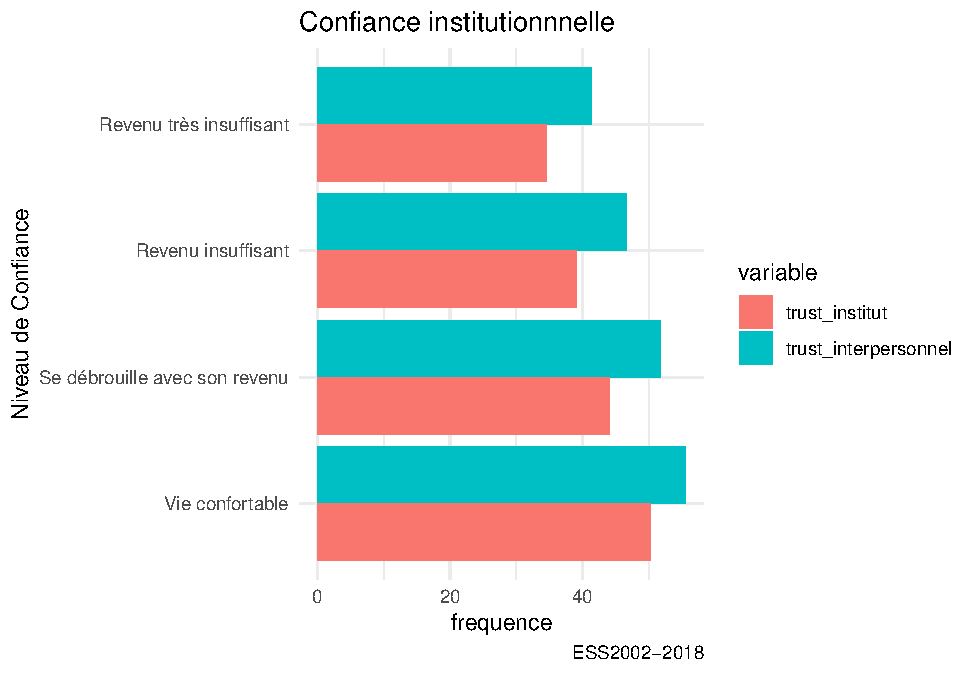
\includegraphics{bookdown-demo_files/figure-latex/0420-1.pdf}

On a une solution mais pas la meilleure, on perd l'idée de variance et ce serait bien d'ajouter des barres d'intervalle de confiances , un diagramme en lignes serait plus élégant. On en profite pour corriger l'aspect des labels peu lisibles en les inclinants, et à choisir une échelle qui omettent les valeur supérieur à 70 et inférieure à 30 pour donner une vision plus respectueuses de la totalité de l'échelle qui va de 0 à 100.

Au passage on emploie à nouveau cowplot pour combiner les graphes, et ici plus précisément partager la légende des deux graphiques.

On observera que si le niveau de confiance diminue avec le revenu, la confiance interpersonnelle est plus forte, et de manière parallèle, à la confiance institutionnelle. On remarquera enfin que c'est pour les revenu les plus faibles que l'estimation est la plus imprécise ou la variance la plus grande.

\begin{Shaded}
\begin{Highlighting}[]
\NormalTok{df_wave2<-df }\OperatorTok\StringTok{ }
\StringTok{  }\KeywordTok{filter}\NormalTok{(cntry}\OperatorTok{==}\StringTok{"FR"} \OperatorTok{&}\StringTok{ }\NormalTok{Year}\OperatorTok{==}\StringTok{"2018"}\NormalTok{)}\OperatorTok
\StringTok{  }\KeywordTok{group_by}\NormalTok{(revenu) }\OperatorTok\StringTok{ }
\StringTok{  }\KeywordTok{mutate}\NormalTok{(}\DataTypeTok{n=}\DecValTok{1}\NormalTok{) }\OperatorTok
\StringTok{  }\KeywordTok{summarise}\NormalTok{(}\DataTypeTok{trust_interpersonnel_se=}\KeywordTok{sd}\NormalTok{(trust_interpersonnel, }\DataTypeTok{na.rm=}\OtherTok{TRUE}\NormalTok{), }\CommentTok{#on calcule l'écartype des deux variables}
            \DataTypeTok{trust_institut_se =}\KeywordTok{sd}\NormalTok{(trust_institut, }\DataTypeTok{na.rm=}\OtherTok{TRUE}\NormalTok{),}
            \DataTypeTok{n=}\KeywordTok{sum}\NormalTok{(n),}
            \DataTypeTok{trust_interpersonnel_se=} \DecValTok{2}\OperatorTok{*}\NormalTok{trust_interpersonnel_se}\OperatorTok{/}\KeywordTok{sqrt}\NormalTok{(n), }\CommentTok{# on calcule l'erreur type d'échantillonnage}
            \DataTypeTok{trust_institut_se=}\DecValTok{2}\OperatorTok{*}\NormalTok{trust_institut_se}\OperatorTok{/}\KeywordTok{sqrt}\NormalTok{(n)}
\NormalTok{            ) }\OperatorTok\StringTok{ }\NormalTok{dplyr}\OperatorTok{::}\KeywordTok{select}\NormalTok{(}\OperatorTok{-}\NormalTok{n) }\OperatorTok
\StringTok{  }\KeywordTok{filter}\NormalTok{(}\OperatorTok{!}\KeywordTok{is.na}\NormalTok{(revenu)) }\OperatorTok\StringTok{ }
\StringTok{  }\KeywordTok{gather}\NormalTok{(variable, value, }\OperatorTok{-}\NormalTok{revenu) }\OperatorTok\StringTok{ }\CommentTok{#on passe en format long}
\StringTok{  }\NormalTok{dplyr}\OperatorTok{::}\KeywordTok{select}\NormalTok{(}\OperatorTok{-}\NormalTok{revenu,}\OperatorTok{-}\NormalTok{variable)}\OperatorTok
\StringTok{  }\KeywordTok{rename}\NormalTok{(}\DataTypeTok{se=}\NormalTok{value)}
  
\NormalTok{df_wave3<-}\KeywordTok{cbind}\NormalTok{(df_wave,df_wave2) }\CommentTok{#on concatène les moyennes et les erreurs types}

\CommentTok{#on peut enfin produire le graphique}

\NormalTok{g06a<-}\KeywordTok{ggplot}\NormalTok{(df_wave3,}\KeywordTok{aes}\NormalTok{(}\DataTypeTok{x=}\NormalTok{revenu,}\DataTypeTok{y=}\NormalTok{value, }\DataTypeTok{group=}\NormalTok{variable))}\OperatorTok{+}
\StringTok{  }\KeywordTok{geom_line}\NormalTok{(}\DataTypeTok{stat=}\StringTok{"identity"}\NormalTok{,}\KeywordTok{aes}\NormalTok{(}\DataTypeTok{color=}\NormalTok{variable), }\DataTypeTok{size=}\FloatTok{1.5}\NormalTok{)}\OperatorTok{+}\StringTok{ }
\StringTok{  }\KeywordTok{geom_errorbar}\NormalTok{(}\KeywordTok{aes}\NormalTok{(}\DataTypeTok{ymin=}\NormalTok{value}\OperatorTok{-}\NormalTok{se, }\DataTypeTok{ymax=}\NormalTok{value}\OperatorTok{+}\NormalTok{se, }\DataTypeTok{color=}\NormalTok{variable), }\DataTypeTok{width=}\NormalTok{.}\DecValTok{2}\NormalTok{,}\DataTypeTok{position=}\KeywordTok{position_dodge}\NormalTok{(}\DecValTok{0}\NormalTok{))}\OperatorTok{+}
\StringTok{  }\KeywordTok{labs}\NormalTok{(}\DataTypeTok{title=} \StringTok{"Confiance et revenu"}\NormalTok{,}\DataTypeTok{y=} \StringTok{"Moyenne"}\NormalTok{,}\DataTypeTok{x=}\OtherTok{NULL}\NormalTok{)}\OperatorTok{+}
\StringTok{  }\KeywordTok{theme}\NormalTok{(}\DataTypeTok{axis.text.x =} \KeywordTok{element_text}\NormalTok{( }\DataTypeTok{angle=}\DecValTok{45}\NormalTok{, }\DataTypeTok{hjust =}\DecValTok{1}\NormalTok{)) }\CommentTok{#on controle l'angle et la position horizontale du label}

  
\NormalTok{g06b<-}\KeywordTok{ggplot}\NormalTok{(df_wave3,}\KeywordTok{aes}\NormalTok{(}\DataTypeTok{x=}\NormalTok{revenu,}\DataTypeTok{y=}\NormalTok{value, }\DataTypeTok{group=}\NormalTok{variable))}\OperatorTok{+}
\StringTok{  }\KeywordTok{geom_line}\NormalTok{(}\DataTypeTok{stat=}\StringTok{"identity"}\NormalTok{,}\KeywordTok{aes}\NormalTok{(}\DataTypeTok{color=}\NormalTok{variable), }\DataTypeTok{size=}\FloatTok{1.5}\NormalTok{)}\OperatorTok{+}\StringTok{ }
\StringTok{  }\KeywordTok{geom_errorbar}\NormalTok{(}\KeywordTok{aes}\NormalTok{(}\DataTypeTok{ymin=}\NormalTok{value}\OperatorTok{-}\NormalTok{se, }\DataTypeTok{ymax=}\NormalTok{value}\OperatorTok{+}\NormalTok{se, }\DataTypeTok{color=}\NormalTok{variable), }\DataTypeTok{width=}\NormalTok{.}\DecValTok{2}\NormalTok{,}\DataTypeTok{position=}\KeywordTok{position_dodge}\NormalTok{(}\DecValTok{0}\NormalTok{))}\OperatorTok{+}
\StringTok{  }\KeywordTok{ylim}\NormalTok{(}\DecValTok{0}\NormalTok{,}\DecValTok{100}\NormalTok{)}\OperatorTok{+}
\StringTok{  }\KeywordTok{labs}\NormalTok{(}\DataTypeTok{title=} \StringTok{""}\NormalTok{,}\DataTypeTok{y=} \StringTok{"Moyenne"}\NormalTok{,}\DataTypeTok{x=}\OtherTok{NULL}\NormalTok{)}\OperatorTok{+}
\StringTok{  }\KeywordTok{theme}\NormalTok{(}\DataTypeTok{axis.text.x =} \KeywordTok{element_text}\NormalTok{( }\DataTypeTok{angle=}\DecValTok{45}\NormalTok{, }\DataTypeTok{hjust =}\DecValTok{1}\NormalTok{)) }\CommentTok{#on controle l'angle et la position horizontale du label}

\NormalTok{prow <-}\StringTok{ }\KeywordTok{plot_grid}\NormalTok{(}
\NormalTok{  g06a }\OperatorTok{+}\StringTok{ }\KeywordTok{theme}\NormalTok{(}\DataTypeTok{legend.position=}\StringTok{"none"}\NormalTok{),}
\NormalTok{  g06b }\OperatorTok{+}\StringTok{ }\KeywordTok{theme}\NormalTok{(}\DataTypeTok{legend.position=}\StringTok{"none"}\NormalTok{),}
  \DataTypeTok{align =} \StringTok{'vh'}\NormalTok{,}
  \DataTypeTok{labels =} \KeywordTok{c}\NormalTok{(}\StringTok{"A"}\NormalTok{, }\StringTok{"B"}\NormalTok{, }\StringTok{"C"}\NormalTok{),}
  \DataTypeTok{hjust =} \DecValTok{-1}\NormalTok{,}
  \DataTypeTok{nrow =} \DecValTok{1}
\NormalTok{)}
\CommentTok{# extract a legend that is laid out horizontally}
\NormalTok{legend_b <-}\StringTok{ }\KeywordTok{get_legend}\NormalTok{(}
\NormalTok{  g06a }\OperatorTok{+}\StringTok{ }
\StringTok{    }\KeywordTok{guides}\NormalTok{(}\DataTypeTok{color =} \KeywordTok{guide_legend}\NormalTok{(}\DataTypeTok{nrow =} \DecValTok{1}\NormalTok{)) }\OperatorTok{+}
\StringTok{    }\KeywordTok{theme}\NormalTok{(}\DataTypeTok{legend.position =} \StringTok{"bottom"}\NormalTok{)}
\NormalTok{)}

\CommentTok{# add the legend underneath the row we made earlier. Give it 10%}
\CommentTok{# of the height of one plot (via rel_heights).}
\KeywordTok{plot_grid}\NormalTok{(prow, legend_b, }\DataTypeTok{ncol =} \DecValTok{1}\NormalTok{, }\DataTypeTok{rel_heights =} \KeywordTok{c}\NormalTok{(}\DecValTok{1}\NormalTok{, }\FloatTok{.1}\NormalTok{))}
\end{Highlighting}
\end{Shaded}

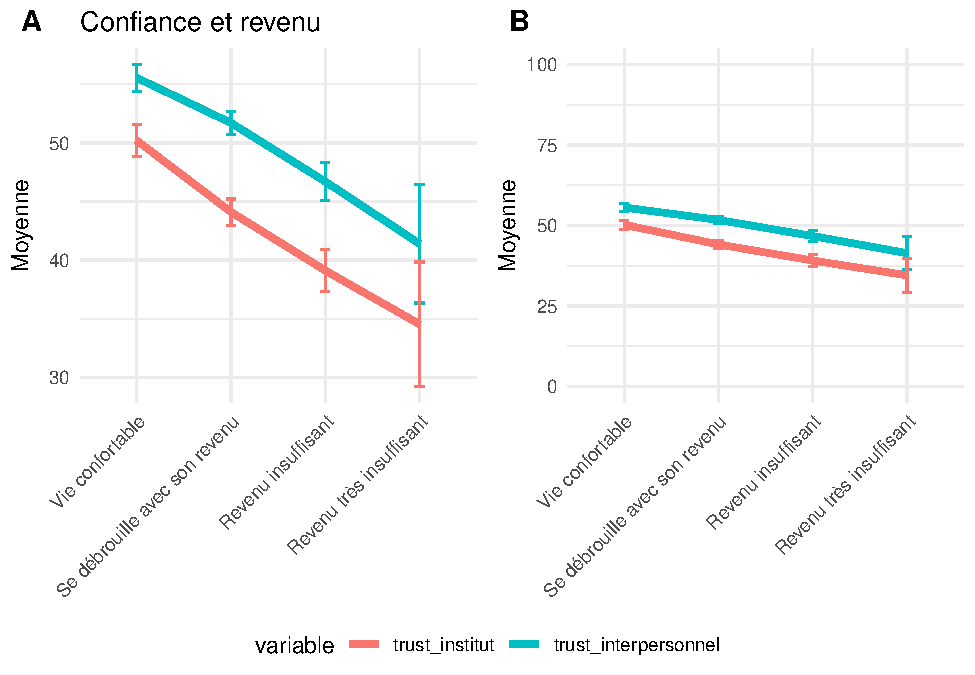
\includegraphics{bookdown-demo_files/figure-latex/0422-1.pdf}

La visualisation est utile, encore faut-il qu'on soit bien certain que les variations ne soit pas le produit du hasard, des fluctuations d'échantillonnage. Si en moyenne la perception du pouvoir d'achat est associée à des moyennes de confiance décroissantes, les différences observées sont-elle significatives? Dans les représentations précédentes c'est le choix de l'échelle qui oriente l'analyse.

On a un besoin d'un test plus objectif. Celui est le très classique test d'analyse de variance (ANOVA).

Celui-çi est le test d'analyse de variance qui consiste à comparer la variance à l'intérieur des groupes ( intra), et la variance entre les moyennes des groupes (inter ou between).

On note qu'ici on introduit la méthode flextable pour présenter des tableaux au formats scientifique. L'astuce ici est d'utiliser aussi xtable.

\begin{Shaded}
\begin{Highlighting}[]
\NormalTok{foo<-df }\OperatorTok\StringTok{ }
\StringTok{  }\KeywordTok{filter}\NormalTok{(cntry}\OperatorTok{==}\StringTok{"FR"} \OperatorTok{&}\StringTok{ }\NormalTok{Year}\OperatorTok{==}\StringTok{"2018"}\NormalTok{) }\OperatorTok\StringTok{ }\KeywordTok{drop_na}\NormalTok{() }\CommentTok{#selection des données}

\NormalTok{fit<-}\KeywordTok{lm}\NormalTok{(trust_institut}\OperatorTok{~}\NormalTok{revenu, foo) }\CommentTok{#calcul du modèle linéaire}

\KeywordTok{anova}\NormalTok{(fit) }\CommentTok{#test d'analyse de variance}
\end{Highlighting}
\end{Shaded}

\begin{verbatim}
## Analysis of Variance Table
## 
## Response: trust_institut
##             Df Sum Sq Mean Sq F value    Pr(>F)    
## revenu       3  27651  9217.1  32.052 < 2.2e-16 ***
## Residuals 1686 484846   287.6                      
## ---
## Signif. codes:  0 '***' 0.001 '**' 0.01 '*' 0.05 '.' 0.1 ' ' 1
\end{verbatim}

\begin{Shaded}
\begin{Highlighting}[]
\KeywordTok{library}\NormalTok{(xtable) }\CommentTok{#xtable transforme en table certains type d'objet dont les résultats de l'anova}
\NormalTok{ft <-}\StringTok{ }\KeywordTok{xtable_to_flextable}\NormalTok{(}\KeywordTok{xtable}\NormalTok{(}\KeywordTok{anova}\NormalTok{(fit)), }\DataTypeTok{hline.after =} \KeywordTok{c}\NormalTok{(}\DecValTok{0}\NormalTok{,}\DecValTok{2}\NormalTok{)) }\CommentTok{#la fonction permet d'exploiter flextable.}
\NormalTok{ft}
\end{Highlighting}
\end{Shaded}

\providecommand{\docline}[3]{\noalign{\global\setlength{\arrayrulewidth}{#1}}\arrayrulecolor[HTML]{#2}\cline{#3}}

\setlength{\tabcolsep}{2pt}

\renewcommand*{\arraystretch}{1.5}

\begin{longtable}[c]{|p{1.01in}|p{0.67in}|p{0.96in}|p{0.91in}|p{0.81in}|p{0.73in}}



\hhline{~~~~~~}

\multicolumn{1}{!{\color[HTML]{000000}\vrule width 0pt}>{\raggedright}p{\dimexpr 1.01in+0\tabcolsep+0\arrayrulewidth}}{\fontsize{11}{11}\selectfont{\textcolor[HTML]{000000}{\global\setmainfont{Arial}{\textbf{}}}}} & \multicolumn{1}{!{\color[HTML]{000000}\vrule width 0pt}>{\raggedleft}p{\dimexpr 0.67in+0\tabcolsep+0\arrayrulewidth}}{\fontsize{11}{11}\selectfont{\textcolor[HTML]{000000}{\global\setmainfont{Arial}{\textbf{Df}}}}} & \multicolumn{1}{!{\color[HTML]{000000}\vrule width 0pt}>{\raggedleft}p{\dimexpr 0.96in+0\tabcolsep+0\arrayrulewidth}}{\fontsize{11}{11}\selectfont{\textcolor[HTML]{000000}{\global\setmainfont{Arial}{\textbf{Sum\ Sq}}}}} & \multicolumn{1}{!{\color[HTML]{000000}\vrule width 0pt}>{\raggedleft}p{\dimexpr 0.91in+0\tabcolsep+0\arrayrulewidth}}{\fontsize{11}{11}\selectfont{\textcolor[HTML]{000000}{\global\setmainfont{Arial}{\textbf{Mean\ Sq}}}}} & \multicolumn{1}{!{\color[HTML]{000000}\vrule width 0pt}>{\raggedleft}p{\dimexpr 0.81in+0\tabcolsep+0\arrayrulewidth}}{\fontsize{11}{11}\selectfont{\textcolor[HTML]{000000}{\global\setmainfont{Arial}{\textbf{F\ value}}}}} & \multicolumn{1}{!{\color[HTML]{000000}\vrule width 0pt}>{\raggedleft}p{\dimexpr 0.73in+0\tabcolsep+0\arrayrulewidth}!{\color[HTML]{000000}\vrule width 0pt}}{\fontsize{11}{11}\selectfont{\textcolor[HTML]{000000}{\global\setmainfont{Arial}{\textbf{Pr(>F)}}}}} \\

\noalign{\global\setlength{\arrayrulewidth}{1pt}}\arrayrulecolor[HTML]{000000}\cline{1-6}

\endfirsthead

\hhline{~~~~~~}

\multicolumn{1}{!{\color[HTML]{000000}\vrule width 0pt}>{\raggedright}p{\dimexpr 1.01in+0\tabcolsep+0\arrayrulewidth}}{\fontsize{11}{11}\selectfont{\textcolor[HTML]{000000}{\global\setmainfont{Arial}{\textbf{}}}}} & \multicolumn{1}{!{\color[HTML]{000000}\vrule width 0pt}>{\raggedleft}p{\dimexpr 0.67in+0\tabcolsep+0\arrayrulewidth}}{\fontsize{11}{11}\selectfont{\textcolor[HTML]{000000}{\global\setmainfont{Arial}{\textbf{Df}}}}} & \multicolumn{1}{!{\color[HTML]{000000}\vrule width 0pt}>{\raggedleft}p{\dimexpr 0.96in+0\tabcolsep+0\arrayrulewidth}}{\fontsize{11}{11}\selectfont{\textcolor[HTML]{000000}{\global\setmainfont{Arial}{\textbf{Sum\ Sq}}}}} & \multicolumn{1}{!{\color[HTML]{000000}\vrule width 0pt}>{\raggedleft}p{\dimexpr 0.91in+0\tabcolsep+0\arrayrulewidth}}{\fontsize{11}{11}\selectfont{\textcolor[HTML]{000000}{\global\setmainfont{Arial}{\textbf{Mean\ Sq}}}}} & \multicolumn{1}{!{\color[HTML]{000000}\vrule width 0pt}>{\raggedleft}p{\dimexpr 0.81in+0\tabcolsep+0\arrayrulewidth}}{\fontsize{11}{11}\selectfont{\textcolor[HTML]{000000}{\global\setmainfont{Arial}{\textbf{F\ value}}}}} & \multicolumn{1}{!{\color[HTML]{000000}\vrule width 0pt}>{\raggedleft}p{\dimexpr 0.73in+0\tabcolsep+0\arrayrulewidth}!{\color[HTML]{000000}\vrule width 0pt}}{\fontsize{11}{11}\selectfont{\textcolor[HTML]{000000}{\global\setmainfont{Arial}{\textbf{Pr(>F)}}}}} \\

\noalign{\global\setlength{\arrayrulewidth}{1pt}}\arrayrulecolor[HTML]{000000}\cline{1-6}\endhead



\multicolumn{1}{!{\color[HTML]{000000}\vrule width 0pt}>{\raggedright}p{\dimexpr 1.01in+0\tabcolsep+0\arrayrulewidth}}{\fontsize{11}{11}\selectfont{\textcolor[HTML]{000000}{\global\setmainfont{Arial}{\textbf{revenu}}}}} & \multicolumn{1}{!{\color[HTML]{000000}\vrule width 0pt}>{\raggedleft}p{\dimexpr 0.67in+0\tabcolsep+0\arrayrulewidth}}{\fontsize{11}{11}\selectfont{\textcolor[HTML]{000000}{\global\setmainfont{Arial}{3}}}} & \multicolumn{1}{!{\color[HTML]{000000}\vrule width 0pt}>{\raggedleft}p{\dimexpr 0.96in+0\tabcolsep+0\arrayrulewidth}}{\fontsize{11}{11}\selectfont{\textcolor[HTML]{000000}{\global\setmainfont{Arial}{27,651.4}}}} & \multicolumn{1}{!{\color[HTML]{000000}\vrule width 0pt}>{\raggedleft}p{\dimexpr 0.91in+0\tabcolsep+0\arrayrulewidth}}{\fontsize{11}{11}\selectfont{\textcolor[HTML]{000000}{\global\setmainfont{Arial}{9,217.1}}}} & \multicolumn{1}{!{\color[HTML]{000000}\vrule width 0pt}>{\raggedleft}p{\dimexpr 0.81in+0\tabcolsep+0\arrayrulewidth}}{\fontsize{11}{11}\selectfont{\textcolor[HTML]{000000}{\global\setmainfont{Arial}{32.1}}}} & \multicolumn{1}{!{\color[HTML]{000000}\vrule width 0pt}>{\raggedleft}p{\dimexpr 0.73in+0\tabcolsep+0\arrayrulewidth}!{\color[HTML]{000000}\vrule width 0pt}}{\fontsize{11}{11}\selectfont{\textcolor[HTML]{000000}{\global\setmainfont{Arial}{0.0}}}} \\





\multicolumn{1}{!{\color[HTML]{000000}\vrule width 0pt}>{\raggedright}p{\dimexpr 1.01in+0\tabcolsep+0\arrayrulewidth}}{\fontsize{11}{11}\selectfont{\textcolor[HTML]{000000}{\global\setmainfont{Arial}{\textbf{Residuals}}}}} & \multicolumn{1}{!{\color[HTML]{000000}\vrule width 0pt}>{\raggedleft}p{\dimexpr 0.67in+0\tabcolsep+0\arrayrulewidth}}{\fontsize{11}{11}\selectfont{\textcolor[HTML]{000000}{\global\setmainfont{Arial}{1,686}}}} & \multicolumn{1}{!{\color[HTML]{000000}\vrule width 0pt}>{\raggedleft}p{\dimexpr 0.96in+0\tabcolsep+0\arrayrulewidth}}{\fontsize{11}{11}\selectfont{\textcolor[HTML]{000000}{\global\setmainfont{Arial}{484,845.7}}}} & \multicolumn{1}{!{\color[HTML]{000000}\vrule width 0pt}>{\raggedleft}p{\dimexpr 0.91in+0\tabcolsep+0\arrayrulewidth}}{\fontsize{11}{11}\selectfont{\textcolor[HTML]{000000}{\global\setmainfont{Arial}{287.6}}}} & \multicolumn{1}{!{\color[HTML]{000000}\vrule width 0pt}>{\raggedleft}p{\dimexpr 0.81in+0\tabcolsep+0\arrayrulewidth}}{\fontsize{11}{11}\selectfont{\textcolor[HTML]{000000}{\global\setmainfont{Arial}{}}}} & \multicolumn{1}{!{\color[HTML]{000000}\vrule width 0pt}>{\raggedleft}p{\dimexpr 0.73in+0\tabcolsep+0\arrayrulewidth}!{\color[HTML]{000000}\vrule width 0pt}}{\fontsize{11}{11}\selectfont{\textcolor[HTML]{000000}{\global\setmainfont{Arial}{}}}} \\

\noalign{\global\setlength{\arrayrulewidth}{1pt}}\arrayrulecolor[HTML]{000000}\cline{1-6}



\end{longtable}

\hypertarget{deux-variables-qualitatives}{%
\subsection{Deux variables qualitatives}\label{deux-variables-qualitatives}}

L'étude de la relation éventuelle entre deux variables qualitative s'apprécie traditionnellement par une méthode de tableau croisé.

\hypertarget{tableau-croisuxe9}{%
\subsubsection{Tableau croisé}\label{tableau-croisuxe9}}

Pour calculer le tableau croisé on utilise la fonction très simple \texttt{table} et la fonction \texttt{prop.table}

\begin{Shaded}
\begin{Highlighting}[]
\NormalTok{t<-}\KeywordTok{table}\NormalTok{(foo}\OperatorTok{$}\NormalTok{revenu,foo}\OperatorTok{$}\NormalTok{habitat)}
\NormalTok{t}
\end{Highlighting}
\end{Shaded}

\begin{verbatim}
##                                
##                                 Big city Suburbs Town Village Countryside
##   Vie confortable                    118      82  161     142          31
##   Se débrouille avec son revenu      120     109  275     227          58
##   Revenu insuffisant                  48      38  129      88          22
##   Revenu très insuffisant              9       5   18      10           0
\end{verbatim}

\begin{Shaded}
\begin{Highlighting}[]
\KeywordTok{prop.table}\NormalTok{(t,}\DecValTok{2}\NormalTok{)}
\end{Highlighting}
\end{Shaded}

\begin{verbatim}
##                                
##                                   Big city    Suburbs       Town    Village
##   Vie confortable               0.40000000 0.35042735 0.27615780 0.30406852
##   Se débrouille avec son revenu 0.40677966 0.46581197 0.47169811 0.48608137
##   Revenu insuffisant            0.16271186 0.16239316 0.22126930 0.18843683
##   Revenu très insuffisant       0.03050847 0.02136752 0.03087479 0.02141328
##                                
##                                 Countryside
##   Vie confortable                0.27927928
##   Se débrouille avec son revenu  0.52252252
##   Revenu insuffisant             0.19819820
##   Revenu très insuffisant        0.00000000
\end{verbatim}

Mais ce n'est pas esthétique, avec la fonction \texttt{proc\_freq} de flextable on obtient une meilleure présentation. Elle nous donne en peu de mots les effectif par cellule, les pourcentages en lignes, et en colonnes.

\begin{Shaded}
\begin{Highlighting}[]
\NormalTok{ft1<-}\StringTok{ }\KeywordTok{proc_freq}\NormalTok{(foo, }\StringTok{"revenu"}\NormalTok{, }\StringTok{"habitat"}\NormalTok{, }\DataTypeTok{include.table_percent =} \OtherTok{FALSE}\NormalTok{,}
                \DataTypeTok{include.row_percent =} \OtherTok{FALSE}\NormalTok{, }\DataTypeTok{include.column_total =} \OtherTok{FALSE}\NormalTok{,}
  \DataTypeTok{include.column_percent =} \OtherTok{TRUE}\NormalTok{)}
\NormalTok{ft1}
\end{Highlighting}
\end{Shaded}

\providecommand{\docline}[3]{\noalign{\global\setlength{\arrayrulewidth}{#1}}\arrayrulecolor[HTML]{#2}\cline{#3}}

\setlength{\tabcolsep}{2pt}

\renewcommand*{\arraystretch}{1.5}

\begin{longtable}[c]{|p{2.34in}|p{1.01in}|p{1.26in}|p{1.26in}|p{1.26in}|p{1.26in}|p{1.10in}|p{0.62in}}



\hhline{~~~~~~~~}

\multicolumn{2}{!{\color[HTML]{FFFFFF}\vrule width 0pt}>{\centering}p{\dimexpr 3.35in+2\tabcolsep+1\arrayrulewidth}}{\fontsize{11}{11}\selectfont{\textcolor[HTML]{000000}{\global\setmainfont{Arial}{\textbf{}}}}} & \multicolumn{6}{!{\color[HTML]{FFFFFF}\vrule width 0pt}>{\centering}p{\dimexpr 6.77in+10\tabcolsep+5\arrayrulewidth}!{\color[HTML]{FFFFFF}\vrule width 0pt}}{\fontsize{11}{11}\selectfont{\textcolor[HTML]{000000}{\global\setmainfont{Arial}{\textbf{habitat}}}}} \\

\noalign{\global\setlength{\arrayrulewidth}{1pt}}\arrayrulecolor[HTML]{000000}\cline{1-8}

\multicolumn{1}{!{\color[HTML]{000000}\vrule width 0pt}>{\centering}p{\dimexpr 2.34in+0\tabcolsep+0\arrayrulewidth}}{\fontsize{11}{11}\selectfont{\textcolor[HTML]{000000}{\global\setmainfont{Arial}{\textbf{revenu}}}}} & \multicolumn{1}{!{\color[HTML]{000000}\vrule width 0pt}>{\centering}p{\dimexpr 1.01in+0\tabcolsep+0\arrayrulewidth}}{\fontsize{11}{11}\selectfont{\textcolor[HTML]{000000}{\global\setmainfont{Arial}{\textbf{label}}}}} & \multicolumn{1}{!{\color[HTML]{000000}\vrule width 0pt}>{\centering}p{\dimexpr 1.26in+0\tabcolsep+0\arrayrulewidth}}{\fontsize{11}{11}\selectfont{\textcolor[HTML]{000000}{\global\setmainfont{Arial}{\textbf{Big\ city}}}}} & \multicolumn{1}{!{\color[HTML]{000000}\vrule width 0pt}>{\centering}p{\dimexpr 1.26in+0\tabcolsep+0\arrayrulewidth}}{\fontsize{11}{11}\selectfont{\textcolor[HTML]{000000}{\global\setmainfont{Arial}{\textbf{Suburbs}}}}} & \multicolumn{1}{!{\color[HTML]{000000}\vrule width 0pt}>{\centering}p{\dimexpr 1.26in+0\tabcolsep+0\arrayrulewidth}}{\fontsize{11}{11}\selectfont{\textcolor[HTML]{000000}{\global\setmainfont{Arial}{\textbf{Town}}}}} & \multicolumn{1}{!{\color[HTML]{000000}\vrule width 0pt}>{\centering}p{\dimexpr 1.26in+0\tabcolsep+0\arrayrulewidth}}{\fontsize{11}{11}\selectfont{\textcolor[HTML]{000000}{\global\setmainfont{Arial}{\textbf{Village}}}}} & \multicolumn{1}{!{\color[HTML]{000000}\vrule width 0pt}>{\centering}p{\dimexpr 1.1in+0\tabcolsep+0\arrayrulewidth}}{\fontsize{11}{11}\selectfont{\textcolor[HTML]{000000}{\global\setmainfont{Arial}{\textbf{Countryside}}}}} & \multicolumn{1}{!{\color[HTML]{000000}\vrule width 0pt}>{\centering}p{\dimexpr 0.62in+0\tabcolsep+0\arrayrulewidth}!{\color[HTML]{000000}\vrule width 0pt}}{\fontsize{11}{11}\selectfont{\textcolor[HTML]{000000}{\global\setmainfont{Arial}{\textbf{Total}}}}} \\

\noalign{\global\setlength{\arrayrulewidth}{2pt}}\arrayrulecolor[HTML]{000000}\cline{1-8}

\endfirsthead

\hhline{~~~~~~~~}

\multicolumn{2}{!{\color[HTML]{FFFFFF}\vrule width 0pt}>{\centering}p{\dimexpr 3.35in+2\tabcolsep+1\arrayrulewidth}}{\fontsize{11}{11}\selectfont{\textcolor[HTML]{000000}{\global\setmainfont{Arial}{\textbf{}}}}} & \multicolumn{6}{!{\color[HTML]{FFFFFF}\vrule width 0pt}>{\centering}p{\dimexpr 6.77in+10\tabcolsep+5\arrayrulewidth}!{\color[HTML]{FFFFFF}\vrule width 0pt}}{\fontsize{11}{11}\selectfont{\textcolor[HTML]{000000}{\global\setmainfont{Arial}{\textbf{habitat}}}}} \\

\noalign{\global\setlength{\arrayrulewidth}{1pt}}\arrayrulecolor[HTML]{000000}\cline{1-8}



\multicolumn{1}{!{\color[HTML]{000000}\vrule width 0pt}>{\centering}p{\dimexpr 2.34in+0\tabcolsep+0\arrayrulewidth}}{\fontsize{11}{11}\selectfont{\textcolor[HTML]{000000}{\global\setmainfont{Arial}{\textbf{revenu}}}}} & \multicolumn{1}{!{\color[HTML]{000000}\vrule width 0pt}>{\centering}p{\dimexpr 1.01in+0\tabcolsep+0\arrayrulewidth}}{\fontsize{11}{11}\selectfont{\textcolor[HTML]{000000}{\global\setmainfont{Arial}{\textbf{label}}}}} & \multicolumn{1}{!{\color[HTML]{000000}\vrule width 0pt}>{\centering}p{\dimexpr 1.26in+0\tabcolsep+0\arrayrulewidth}}{\fontsize{11}{11}\selectfont{\textcolor[HTML]{000000}{\global\setmainfont{Arial}{\textbf{Big\ city}}}}} & \multicolumn{1}{!{\color[HTML]{000000}\vrule width 0pt}>{\centering}p{\dimexpr 1.26in+0\tabcolsep+0\arrayrulewidth}}{\fontsize{11}{11}\selectfont{\textcolor[HTML]{000000}{\global\setmainfont{Arial}{\textbf{Suburbs}}}}} & \multicolumn{1}{!{\color[HTML]{000000}\vrule width 0pt}>{\centering}p{\dimexpr 1.26in+0\tabcolsep+0\arrayrulewidth}}{\fontsize{11}{11}\selectfont{\textcolor[HTML]{000000}{\global\setmainfont{Arial}{\textbf{Town}}}}} & \multicolumn{1}{!{\color[HTML]{000000}\vrule width 0pt}>{\centering}p{\dimexpr 1.26in+0\tabcolsep+0\arrayrulewidth}}{\fontsize{11}{11}\selectfont{\textcolor[HTML]{000000}{\global\setmainfont{Arial}{\textbf{Village}}}}} & \multicolumn{1}{!{\color[HTML]{000000}\vrule width 0pt}>{\centering}p{\dimexpr 1.1in+0\tabcolsep+0\arrayrulewidth}}{\fontsize{11}{11}\selectfont{\textcolor[HTML]{000000}{\global\setmainfont{Arial}{\textbf{Countryside}}}}} & \multicolumn{1}{!{\color[HTML]{000000}\vrule width 0pt}>{\centering}p{\dimexpr 0.62in+0\tabcolsep+0\arrayrulewidth}!{\color[HTML]{000000}\vrule width 0pt}}{\fontsize{11}{11}\selectfont{\textcolor[HTML]{000000}{\global\setmainfont{Arial}{\textbf{Total}}}}} \\

\noalign{\global\setlength{\arrayrulewidth}{2pt}}\arrayrulecolor[HTML]{000000}\cline{1-8}\endhead



\multicolumn{1}{!{\color[HTML]{000000}\vrule width 0pt}>{\centering}p{\dimexpr 2.34in+0\tabcolsep+0\arrayrulewidth}}{} & \multicolumn{1}{!{\color[HTML]{000000}\vrule width 0pt}>{\centering}p{\dimexpr 1.01in+0\tabcolsep+0\arrayrulewidth}}{\fontsize{11}{11}\selectfont{\textcolor[HTML]{000000}{\global\setmainfont{Arial}{Frequency}}}} & \multicolumn{1}{!{\color[HTML]{000000}\vrule width 0pt}>{\centering}p{\dimexpr 1.26in+0\tabcolsep+0\arrayrulewidth}}{\fontsize{11}{11}\selectfont{\textcolor[HTML]{000000}{\global\setmainfont{Arial}{118}}}} & \multicolumn{1}{!{\color[HTML]{000000}\vrule width 0pt}>{\centering}p{\dimexpr 1.26in+0\tabcolsep+0\arrayrulewidth}}{\fontsize{11}{11}\selectfont{\textcolor[HTML]{000000}{\global\setmainfont{Arial}{82}}}} & \multicolumn{1}{!{\color[HTML]{000000}\vrule width 0pt}>{\centering}p{\dimexpr 1.26in+0\tabcolsep+0\arrayrulewidth}}{\fontsize{11}{11}\selectfont{\textcolor[HTML]{000000}{\global\setmainfont{Arial}{161}}}} & \multicolumn{1}{!{\color[HTML]{000000}\vrule width 0pt}>{\centering}p{\dimexpr 1.26in+0\tabcolsep+0\arrayrulewidth}}{\fontsize{11}{11}\selectfont{\textcolor[HTML]{000000}{\global\setmainfont{Arial}{142}}}} & \multicolumn{1}{!{\color[HTML]{000000}\vrule width 0pt}>{\centering}p{\dimexpr 1.1in+0\tabcolsep+0\arrayrulewidth}}{\fontsize{11}{11}\selectfont{\textcolor[HTML]{000000}{\global\setmainfont{Arial}{31}}}} & \multicolumn{1}{!{\color[HTML]{000000}\vrule width 0pt}>{\centering}p{\dimexpr 0.62in+0\tabcolsep+0\arrayrulewidth}!{\color[HTML]{000000}\vrule width 0pt}}{\fontsize{11}{11}\selectfont{\textcolor[HTML]{000000}{\global\setmainfont{Arial}{534}}}} \\





\multicolumn{1}{!{\color[HTML]{000000}\vrule width 0pt}>{\centering}p{\dimexpr 2.34in+0\tabcolsep+0\arrayrulewidth}}{\multirow[t]{-2}{*}{\fontsize{11}{11}\selectfont{\textcolor[HTML]{000000}{\global\setmainfont{Arial}{\textbf{Vie\ confortable}}}}}} & \multicolumn{1}{!{\color[HTML]{000000}\vrule width 0pt}>{\centering}p{\dimexpr 1.01in+0\tabcolsep+0\arrayrulewidth}}{\fontsize{11}{11}\selectfont{\textcolor[HTML]{000000}{\global\setmainfont{Arial}{Col\ Pct}}}} & \multicolumn{1}{!{\color[HTML]{000000}\vrule width 0pt}>{\centering}p{\dimexpr 1.26in+0\tabcolsep+0\arrayrulewidth}}{\fontsize{11}{11}\selectfont{\textcolor[HTML]{000000}{\global\setmainfont{Arial}{40\%}}}} & \multicolumn{1}{!{\color[HTML]{000000}\vrule width 0pt}>{\centering}p{\dimexpr 1.26in+0\tabcolsep+0\arrayrulewidth}}{\fontsize{11}{11}\selectfont{\textcolor[HTML]{000000}{\global\setmainfont{Arial}{35.04\%}}}} & \multicolumn{1}{!{\color[HTML]{000000}\vrule width 0pt}>{\centering}p{\dimexpr 1.26in+0\tabcolsep+0\arrayrulewidth}}{\fontsize{11}{11}\selectfont{\textcolor[HTML]{000000}{\global\setmainfont{Arial}{27.62\%}}}} & \multicolumn{1}{!{\color[HTML]{000000}\vrule width 0pt}>{\centering}p{\dimexpr 1.26in+0\tabcolsep+0\arrayrulewidth}}{\fontsize{11}{11}\selectfont{\textcolor[HTML]{000000}{\global\setmainfont{Arial}{30.41\%}}}} & \multicolumn{1}{!{\color[HTML]{000000}\vrule width 0pt}>{\centering}p{\dimexpr 1.1in+0\tabcolsep+0\arrayrulewidth}}{\fontsize{11}{11}\selectfont{\textcolor[HTML]{000000}{\global\setmainfont{Arial}{27.93\%}}}} & \multicolumn{1}{!{\color[HTML]{000000}\vrule width 0pt}>{\centering}p{\dimexpr 0.62in+0\tabcolsep+0\arrayrulewidth}!{\color[HTML]{000000}\vrule width 0pt}}{\fontsize{11}{11}\selectfont{\textcolor[HTML]{000000}{\global\setmainfont{Arial}{}}}} \\





\multicolumn{1}{!{\color[HTML]{000000}\vrule width 0pt}>{\centering}p{\dimexpr 2.34in+0\tabcolsep+0\arrayrulewidth}}{} & \multicolumn{1}{!{\color[HTML]{000000}\vrule width 0pt}>{\centering}p{\dimexpr 1.01in+0\tabcolsep+0\arrayrulewidth}}{\fontsize{11}{11}\selectfont{\textcolor[HTML]{000000}{\global\setmainfont{Arial}{Frequency}}}} & \multicolumn{1}{!{\color[HTML]{000000}\vrule width 0pt}>{\centering}p{\dimexpr 1.26in+0\tabcolsep+0\arrayrulewidth}}{\fontsize{11}{11}\selectfont{\textcolor[HTML]{000000}{\global\setmainfont{Arial}{120}}}} & \multicolumn{1}{!{\color[HTML]{000000}\vrule width 0pt}>{\centering}p{\dimexpr 1.26in+0\tabcolsep+0\arrayrulewidth}}{\fontsize{11}{11}\selectfont{\textcolor[HTML]{000000}{\global\setmainfont{Arial}{109}}}} & \multicolumn{1}{!{\color[HTML]{000000}\vrule width 0pt}>{\centering}p{\dimexpr 1.26in+0\tabcolsep+0\arrayrulewidth}}{\fontsize{11}{11}\selectfont{\textcolor[HTML]{000000}{\global\setmainfont{Arial}{275}}}} & \multicolumn{1}{!{\color[HTML]{000000}\vrule width 0pt}>{\centering}p{\dimexpr 1.26in+0\tabcolsep+0\arrayrulewidth}}{\fontsize{11}{11}\selectfont{\textcolor[HTML]{000000}{\global\setmainfont{Arial}{227}}}} & \multicolumn{1}{!{\color[HTML]{000000}\vrule width 0pt}>{\centering}p{\dimexpr 1.1in+0\tabcolsep+0\arrayrulewidth}}{\fontsize{11}{11}\selectfont{\textcolor[HTML]{000000}{\global\setmainfont{Arial}{58}}}} & \multicolumn{1}{!{\color[HTML]{000000}\vrule width 0pt}>{\centering}p{\dimexpr 0.62in+0\tabcolsep+0\arrayrulewidth}!{\color[HTML]{000000}\vrule width 0pt}}{\fontsize{11}{11}\selectfont{\textcolor[HTML]{000000}{\global\setmainfont{Arial}{789}}}} \\





\multicolumn{1}{!{\color[HTML]{000000}\vrule width 0pt}>{\centering}p{\dimexpr 2.34in+0\tabcolsep+0\arrayrulewidth}}{\multirow[t]{-2}{*}{\fontsize{11}{11}\selectfont{\textcolor[HTML]{000000}{\global\setmainfont{Arial}{\textbf{Se\ débrouille\ avec\ son\ revenu}}}}}} & \multicolumn{1}{!{\color[HTML]{000000}\vrule width 0pt}>{\centering}p{\dimexpr 1.01in+0\tabcolsep+0\arrayrulewidth}}{\fontsize{11}{11}\selectfont{\textcolor[HTML]{000000}{\global\setmainfont{Arial}{Col\ Pct}}}} & \multicolumn{1}{!{\color[HTML]{000000}\vrule width 0pt}>{\centering}p{\dimexpr 1.26in+0\tabcolsep+0\arrayrulewidth}}{\fontsize{11}{11}\selectfont{\textcolor[HTML]{000000}{\global\setmainfont{Arial}{40.68\%}}}} & \multicolumn{1}{!{\color[HTML]{000000}\vrule width 0pt}>{\centering}p{\dimexpr 1.26in+0\tabcolsep+0\arrayrulewidth}}{\fontsize{11}{11}\selectfont{\textcolor[HTML]{000000}{\global\setmainfont{Arial}{46.58\%}}}} & \multicolumn{1}{!{\color[HTML]{000000}\vrule width 0pt}>{\centering}p{\dimexpr 1.26in+0\tabcolsep+0\arrayrulewidth}}{\fontsize{11}{11}\selectfont{\textcolor[HTML]{000000}{\global\setmainfont{Arial}{47.17\%}}}} & \multicolumn{1}{!{\color[HTML]{000000}\vrule width 0pt}>{\centering}p{\dimexpr 1.26in+0\tabcolsep+0\arrayrulewidth}}{\fontsize{11}{11}\selectfont{\textcolor[HTML]{000000}{\global\setmainfont{Arial}{48.61\%}}}} & \multicolumn{1}{!{\color[HTML]{000000}\vrule width 0pt}>{\centering}p{\dimexpr 1.1in+0\tabcolsep+0\arrayrulewidth}}{\fontsize{11}{11}\selectfont{\textcolor[HTML]{000000}{\global\setmainfont{Arial}{52.25\%}}}} & \multicolumn{1}{!{\color[HTML]{000000}\vrule width 0pt}>{\centering}p{\dimexpr 0.62in+0\tabcolsep+0\arrayrulewidth}!{\color[HTML]{000000}\vrule width 0pt}}{\fontsize{11}{11}\selectfont{\textcolor[HTML]{000000}{\global\setmainfont{Arial}{}}}} \\





\multicolumn{1}{!{\color[HTML]{000000}\vrule width 0pt}>{\centering}p{\dimexpr 2.34in+0\tabcolsep+0\arrayrulewidth}}{} & \multicolumn{1}{!{\color[HTML]{000000}\vrule width 0pt}>{\centering}p{\dimexpr 1.01in+0\tabcolsep+0\arrayrulewidth}}{\fontsize{11}{11}\selectfont{\textcolor[HTML]{000000}{\global\setmainfont{Arial}{Frequency}}}} & \multicolumn{1}{!{\color[HTML]{000000}\vrule width 0pt}>{\centering}p{\dimexpr 1.26in+0\tabcolsep+0\arrayrulewidth}}{\fontsize{11}{11}\selectfont{\textcolor[HTML]{000000}{\global\setmainfont{Arial}{48}}}} & \multicolumn{1}{!{\color[HTML]{000000}\vrule width 0pt}>{\centering}p{\dimexpr 1.26in+0\tabcolsep+0\arrayrulewidth}}{\fontsize{11}{11}\selectfont{\textcolor[HTML]{000000}{\global\setmainfont{Arial}{38}}}} & \multicolumn{1}{!{\color[HTML]{000000}\vrule width 0pt}>{\centering}p{\dimexpr 1.26in+0\tabcolsep+0\arrayrulewidth}}{\fontsize{11}{11}\selectfont{\textcolor[HTML]{000000}{\global\setmainfont{Arial}{129}}}} & \multicolumn{1}{!{\color[HTML]{000000}\vrule width 0pt}>{\centering}p{\dimexpr 1.26in+0\tabcolsep+0\arrayrulewidth}}{\fontsize{11}{11}\selectfont{\textcolor[HTML]{000000}{\global\setmainfont{Arial}{88}}}} & \multicolumn{1}{!{\color[HTML]{000000}\vrule width 0pt}>{\centering}p{\dimexpr 1.1in+0\tabcolsep+0\arrayrulewidth}}{\fontsize{11}{11}\selectfont{\textcolor[HTML]{000000}{\global\setmainfont{Arial}{22}}}} & \multicolumn{1}{!{\color[HTML]{000000}\vrule width 0pt}>{\centering}p{\dimexpr 0.62in+0\tabcolsep+0\arrayrulewidth}!{\color[HTML]{000000}\vrule width 0pt}}{\fontsize{11}{11}\selectfont{\textcolor[HTML]{000000}{\global\setmainfont{Arial}{325}}}} \\





\multicolumn{1}{!{\color[HTML]{000000}\vrule width 0pt}>{\centering}p{\dimexpr 2.34in+0\tabcolsep+0\arrayrulewidth}}{\multirow[t]{-2}{*}{\fontsize{11}{11}\selectfont{\textcolor[HTML]{000000}{\global\setmainfont{Arial}{\textbf{Revenu\ insuffisant}}}}}} & \multicolumn{1}{!{\color[HTML]{000000}\vrule width 0pt}>{\centering}p{\dimexpr 1.01in+0\tabcolsep+0\arrayrulewidth}}{\fontsize{11}{11}\selectfont{\textcolor[HTML]{000000}{\global\setmainfont{Arial}{Col\ Pct}}}} & \multicolumn{1}{!{\color[HTML]{000000}\vrule width 0pt}>{\centering}p{\dimexpr 1.26in+0\tabcolsep+0\arrayrulewidth}}{\fontsize{11}{11}\selectfont{\textcolor[HTML]{000000}{\global\setmainfont{Arial}{16.27\%}}}} & \multicolumn{1}{!{\color[HTML]{000000}\vrule width 0pt}>{\centering}p{\dimexpr 1.26in+0\tabcolsep+0\arrayrulewidth}}{\fontsize{11}{11}\selectfont{\textcolor[HTML]{000000}{\global\setmainfont{Arial}{16.24\%}}}} & \multicolumn{1}{!{\color[HTML]{000000}\vrule width 0pt}>{\centering}p{\dimexpr 1.26in+0\tabcolsep+0\arrayrulewidth}}{\fontsize{11}{11}\selectfont{\textcolor[HTML]{000000}{\global\setmainfont{Arial}{22.13\%}}}} & \multicolumn{1}{!{\color[HTML]{000000}\vrule width 0pt}>{\centering}p{\dimexpr 1.26in+0\tabcolsep+0\arrayrulewidth}}{\fontsize{11}{11}\selectfont{\textcolor[HTML]{000000}{\global\setmainfont{Arial}{18.84\%}}}} & \multicolumn{1}{!{\color[HTML]{000000}\vrule width 0pt}>{\centering}p{\dimexpr 1.1in+0\tabcolsep+0\arrayrulewidth}}{\fontsize{11}{11}\selectfont{\textcolor[HTML]{000000}{\global\setmainfont{Arial}{19.82\%}}}} & \multicolumn{1}{!{\color[HTML]{000000}\vrule width 0pt}>{\centering}p{\dimexpr 0.62in+0\tabcolsep+0\arrayrulewidth}!{\color[HTML]{000000}\vrule width 0pt}}{\fontsize{11}{11}\selectfont{\textcolor[HTML]{000000}{\global\setmainfont{Arial}{}}}} \\





\multicolumn{1}{!{\color[HTML]{000000}\vrule width 0pt}>{\centering}p{\dimexpr 2.34in+0\tabcolsep+0\arrayrulewidth}}{} & \multicolumn{1}{!{\color[HTML]{000000}\vrule width 0pt}>{\centering}p{\dimexpr 1.01in+0\tabcolsep+0\arrayrulewidth}}{\fontsize{11}{11}\selectfont{\textcolor[HTML]{000000}{\global\setmainfont{Arial}{Frequency}}}} & \multicolumn{1}{!{\color[HTML]{000000}\vrule width 0pt}>{\centering}p{\dimexpr 1.26in+0\tabcolsep+0\arrayrulewidth}}{\fontsize{11}{11}\selectfont{\textcolor[HTML]{000000}{\global\setmainfont{Arial}{9}}}} & \multicolumn{1}{!{\color[HTML]{000000}\vrule width 0pt}>{\centering}p{\dimexpr 1.26in+0\tabcolsep+0\arrayrulewidth}}{\fontsize{11}{11}\selectfont{\textcolor[HTML]{000000}{\global\setmainfont{Arial}{5}}}} & \multicolumn{1}{!{\color[HTML]{000000}\vrule width 0pt}>{\centering}p{\dimexpr 1.26in+0\tabcolsep+0\arrayrulewidth}}{\fontsize{11}{11}\selectfont{\textcolor[HTML]{000000}{\global\setmainfont{Arial}{18}}}} & \multicolumn{1}{!{\color[HTML]{000000}\vrule width 0pt}>{\centering}p{\dimexpr 1.26in+0\tabcolsep+0\arrayrulewidth}}{\fontsize{11}{11}\selectfont{\textcolor[HTML]{000000}{\global\setmainfont{Arial}{10}}}} & \multicolumn{1}{!{\color[HTML]{000000}\vrule width 0pt}>{\centering}p{\dimexpr 1.1in+0\tabcolsep+0\arrayrulewidth}}{\fontsize{11}{11}\selectfont{\textcolor[HTML]{000000}{\global\setmainfont{Arial}{0}}}} & \multicolumn{1}{!{\color[HTML]{000000}\vrule width 0pt}>{\centering}p{\dimexpr 0.62in+0\tabcolsep+0\arrayrulewidth}!{\color[HTML]{000000}\vrule width 0pt}}{\fontsize{11}{11}\selectfont{\textcolor[HTML]{000000}{\global\setmainfont{Arial}{42}}}} \\





\multicolumn{1}{!{\color[HTML]{000000}\vrule width 0pt}>{\centering}p{\dimexpr 2.34in+0\tabcolsep+0\arrayrulewidth}}{\multirow[t]{-2}{*}{\fontsize{11}{11}\selectfont{\textcolor[HTML]{000000}{\global\setmainfont{Arial}{\textbf{Revenu\ très\ insuffisant}}}}}} & \multicolumn{1}{!{\color[HTML]{000000}\vrule width 0pt}>{\centering}p{\dimexpr 1.01in+0\tabcolsep+0\arrayrulewidth}}{\fontsize{11}{11}\selectfont{\textcolor[HTML]{000000}{\global\setmainfont{Arial}{Col\ Pct}}}} & \multicolumn{1}{!{\color[HTML]{000000}\vrule width 0pt}>{\centering}p{\dimexpr 1.26in+0\tabcolsep+0\arrayrulewidth}}{\fontsize{11}{11}\selectfont{\textcolor[HTML]{000000}{\global\setmainfont{Arial}{3.05\%}}}} & \multicolumn{1}{!{\color[HTML]{000000}\vrule width 0pt}>{\centering}p{\dimexpr 1.26in+0\tabcolsep+0\arrayrulewidth}}{\fontsize{11}{11}\selectfont{\textcolor[HTML]{000000}{\global\setmainfont{Arial}{2.14\%}}}} & \multicolumn{1}{!{\color[HTML]{000000}\vrule width 0pt}>{\centering}p{\dimexpr 1.26in+0\tabcolsep+0\arrayrulewidth}}{\fontsize{11}{11}\selectfont{\textcolor[HTML]{000000}{\global\setmainfont{Arial}{3.09\%}}}} & \multicolumn{1}{!{\color[HTML]{000000}\vrule width 0pt}>{\centering}p{\dimexpr 1.26in+0\tabcolsep+0\arrayrulewidth}}{\fontsize{11}{11}\selectfont{\textcolor[HTML]{000000}{\global\setmainfont{Arial}{2.14\%}}}} & \multicolumn{1}{!{\color[HTML]{000000}\vrule width 0pt}>{\centering}p{\dimexpr 1.1in+0\tabcolsep+0\arrayrulewidth}}{\fontsize{11}{11}\selectfont{\textcolor[HTML]{000000}{\global\setmainfont{Arial}{0\%}}}} & \multicolumn{1}{!{\color[HTML]{000000}\vrule width 0pt}>{\centering}p{\dimexpr 0.62in+0\tabcolsep+0\arrayrulewidth}!{\color[HTML]{000000}\vrule width 0pt}}{\fontsize{11}{11}\selectfont{\textcolor[HTML]{000000}{\global\setmainfont{Arial}{}}}} \\

\noalign{\global\setlength{\arrayrulewidth}{2pt}}\arrayrulecolor[HTML]{666666}\cline{1-8}



\end{longtable}

\begin{Shaded}
\begin{Highlighting}[]
\NormalTok{ft2<-}\StringTok{ }\KeywordTok{proc_freq}\NormalTok{(foo, }\StringTok{"revenu"}\NormalTok{, }\StringTok{"habitat"}\NormalTok{, }\DataTypeTok{include.table_percent =} \OtherTok{FALSE}\NormalTok{,}
                \DataTypeTok{include.row_percent =} \OtherTok{TRUE}\NormalTok{,}
  \DataTypeTok{include.column_percent =} \OtherTok{FALSE}\NormalTok{)}
\NormalTok{ft2}
\end{Highlighting}
\end{Shaded}

\providecommand{\docline}[3]{\noalign{\global\setlength{\arrayrulewidth}{#1}}\arrayrulecolor[HTML]{#2}\cline{#3}}

\setlength{\tabcolsep}{2pt}

\renewcommand*{\arraystretch}{1.5}

\begin{longtable}[c]{|p{2.34in}|p{1.01in}|p{1.18in}|p{1.18in}|p{1.18in}|p{1.18in}|p{1.26in}|p{0.67in}}



\hhline{~~~~~~~~}

\multicolumn{2}{!{\color[HTML]{FFFFFF}\vrule width 0pt}>{\centering}p{\dimexpr 3.35in+2\tabcolsep+1\arrayrulewidth}}{\fontsize{11}{11}\selectfont{\textcolor[HTML]{000000}{\global\setmainfont{Arial}{\textbf{}}}}} & \multicolumn{6}{!{\color[HTML]{FFFFFF}\vrule width 0pt}>{\centering}p{\dimexpr 6.64in+10\tabcolsep+5\arrayrulewidth}!{\color[HTML]{FFFFFF}\vrule width 0pt}}{\fontsize{11}{11}\selectfont{\textcolor[HTML]{000000}{\global\setmainfont{Arial}{\textbf{habitat}}}}} \\

\noalign{\global\setlength{\arrayrulewidth}{1pt}}\arrayrulecolor[HTML]{000000}\cline{1-8}

\multicolumn{1}{!{\color[HTML]{000000}\vrule width 0pt}>{\centering}p{\dimexpr 2.34in+0\tabcolsep+0\arrayrulewidth}}{\fontsize{11}{11}\selectfont{\textcolor[HTML]{000000}{\global\setmainfont{Arial}{\textbf{revenu}}}}} & \multicolumn{1}{!{\color[HTML]{000000}\vrule width 0pt}>{\centering}p{\dimexpr 1.01in+0\tabcolsep+0\arrayrulewidth}}{\fontsize{11}{11}\selectfont{\textcolor[HTML]{000000}{\global\setmainfont{Arial}{\textbf{label}}}}} & \multicolumn{1}{!{\color[HTML]{000000}\vrule width 0pt}>{\centering}p{\dimexpr 1.18in+0\tabcolsep+0\arrayrulewidth}}{\fontsize{11}{11}\selectfont{\textcolor[HTML]{000000}{\global\setmainfont{Arial}{\textbf{Big\ city}}}}} & \multicolumn{1}{!{\color[HTML]{000000}\vrule width 0pt}>{\centering}p{\dimexpr 1.18in+0\tabcolsep+0\arrayrulewidth}}{\fontsize{11}{11}\selectfont{\textcolor[HTML]{000000}{\global\setmainfont{Arial}{\textbf{Suburbs}}}}} & \multicolumn{1}{!{\color[HTML]{000000}\vrule width 0pt}>{\centering}p{\dimexpr 1.18in+0\tabcolsep+0\arrayrulewidth}}{\fontsize{11}{11}\selectfont{\textcolor[HTML]{000000}{\global\setmainfont{Arial}{\textbf{Town}}}}} & \multicolumn{1}{!{\color[HTML]{000000}\vrule width 0pt}>{\centering}p{\dimexpr 1.18in+0\tabcolsep+0\arrayrulewidth}}{\fontsize{11}{11}\selectfont{\textcolor[HTML]{000000}{\global\setmainfont{Arial}{\textbf{Village}}}}} & \multicolumn{1}{!{\color[HTML]{000000}\vrule width 0pt}>{\centering}p{\dimexpr 1.26in+0\tabcolsep+0\arrayrulewidth}}{\fontsize{11}{11}\selectfont{\textcolor[HTML]{000000}{\global\setmainfont{Arial}{\textbf{Countryside}}}}} & \multicolumn{1}{!{\color[HTML]{000000}\vrule width 0pt}>{\centering}p{\dimexpr 0.67in+0\tabcolsep+0\arrayrulewidth}!{\color[HTML]{000000}\vrule width 0pt}}{\fontsize{11}{11}\selectfont{\textcolor[HTML]{000000}{\global\setmainfont{Arial}{\textbf{Total}}}}} \\

\noalign{\global\setlength{\arrayrulewidth}{2pt}}\arrayrulecolor[HTML]{000000}\cline{1-8}

\endfirsthead

\hhline{~~~~~~~~}

\multicolumn{2}{!{\color[HTML]{FFFFFF}\vrule width 0pt}>{\centering}p{\dimexpr 3.35in+2\tabcolsep+1\arrayrulewidth}}{\fontsize{11}{11}\selectfont{\textcolor[HTML]{000000}{\global\setmainfont{Arial}{\textbf{}}}}} & \multicolumn{6}{!{\color[HTML]{FFFFFF}\vrule width 0pt}>{\centering}p{\dimexpr 6.64in+10\tabcolsep+5\arrayrulewidth}!{\color[HTML]{FFFFFF}\vrule width 0pt}}{\fontsize{11}{11}\selectfont{\textcolor[HTML]{000000}{\global\setmainfont{Arial}{\textbf{habitat}}}}} \\

\noalign{\global\setlength{\arrayrulewidth}{1pt}}\arrayrulecolor[HTML]{000000}\cline{1-8}



\multicolumn{1}{!{\color[HTML]{000000}\vrule width 0pt}>{\centering}p{\dimexpr 2.34in+0\tabcolsep+0\arrayrulewidth}}{\fontsize{11}{11}\selectfont{\textcolor[HTML]{000000}{\global\setmainfont{Arial}{\textbf{revenu}}}}} & \multicolumn{1}{!{\color[HTML]{000000}\vrule width 0pt}>{\centering}p{\dimexpr 1.01in+0\tabcolsep+0\arrayrulewidth}}{\fontsize{11}{11}\selectfont{\textcolor[HTML]{000000}{\global\setmainfont{Arial}{\textbf{label}}}}} & \multicolumn{1}{!{\color[HTML]{000000}\vrule width 0pt}>{\centering}p{\dimexpr 1.18in+0\tabcolsep+0\arrayrulewidth}}{\fontsize{11}{11}\selectfont{\textcolor[HTML]{000000}{\global\setmainfont{Arial}{\textbf{Big\ city}}}}} & \multicolumn{1}{!{\color[HTML]{000000}\vrule width 0pt}>{\centering}p{\dimexpr 1.18in+0\tabcolsep+0\arrayrulewidth}}{\fontsize{11}{11}\selectfont{\textcolor[HTML]{000000}{\global\setmainfont{Arial}{\textbf{Suburbs}}}}} & \multicolumn{1}{!{\color[HTML]{000000}\vrule width 0pt}>{\centering}p{\dimexpr 1.18in+0\tabcolsep+0\arrayrulewidth}}{\fontsize{11}{11}\selectfont{\textcolor[HTML]{000000}{\global\setmainfont{Arial}{\textbf{Town}}}}} & \multicolumn{1}{!{\color[HTML]{000000}\vrule width 0pt}>{\centering}p{\dimexpr 1.18in+0\tabcolsep+0\arrayrulewidth}}{\fontsize{11}{11}\selectfont{\textcolor[HTML]{000000}{\global\setmainfont{Arial}{\textbf{Village}}}}} & \multicolumn{1}{!{\color[HTML]{000000}\vrule width 0pt}>{\centering}p{\dimexpr 1.26in+0\tabcolsep+0\arrayrulewidth}}{\fontsize{11}{11}\selectfont{\textcolor[HTML]{000000}{\global\setmainfont{Arial}{\textbf{Countryside}}}}} & \multicolumn{1}{!{\color[HTML]{000000}\vrule width 0pt}>{\centering}p{\dimexpr 0.67in+0\tabcolsep+0\arrayrulewidth}!{\color[HTML]{000000}\vrule width 0pt}}{\fontsize{11}{11}\selectfont{\textcolor[HTML]{000000}{\global\setmainfont{Arial}{\textbf{Total}}}}} \\

\noalign{\global\setlength{\arrayrulewidth}{2pt}}\arrayrulecolor[HTML]{000000}\cline{1-8}\endhead



\multicolumn{1}{!{\color[HTML]{000000}\vrule width 0pt}>{\centering}p{\dimexpr 2.34in+0\tabcolsep+0\arrayrulewidth}}{} & \multicolumn{1}{!{\color[HTML]{000000}\vrule width 0pt}>{\centering}p{\dimexpr 1.01in+0\tabcolsep+0\arrayrulewidth}}{\fontsize{11}{11}\selectfont{\textcolor[HTML]{000000}{\global\setmainfont{Arial}{Frequency}}}} & \multicolumn{1}{!{\color[HTML]{000000}\vrule width 0pt}>{\centering}p{\dimexpr 1.18in+0\tabcolsep+0\arrayrulewidth}}{\fontsize{11}{11}\selectfont{\textcolor[HTML]{000000}{\global\setmainfont{Arial}{118}}}} & \multicolumn{1}{!{\color[HTML]{000000}\vrule width 0pt}>{\centering}p{\dimexpr 1.18in+0\tabcolsep+0\arrayrulewidth}}{\fontsize{11}{11}\selectfont{\textcolor[HTML]{000000}{\global\setmainfont{Arial}{82}}}} & \multicolumn{1}{!{\color[HTML]{000000}\vrule width 0pt}>{\centering}p{\dimexpr 1.18in+0\tabcolsep+0\arrayrulewidth}}{\fontsize{11}{11}\selectfont{\textcolor[HTML]{000000}{\global\setmainfont{Arial}{161}}}} & \multicolumn{1}{!{\color[HTML]{000000}\vrule width 0pt}>{\centering}p{\dimexpr 1.18in+0\tabcolsep+0\arrayrulewidth}}{\fontsize{11}{11}\selectfont{\textcolor[HTML]{000000}{\global\setmainfont{Arial}{142}}}} & \multicolumn{1}{!{\color[HTML]{000000}\vrule width 0pt}>{\centering}p{\dimexpr 1.26in+0\tabcolsep+0\arrayrulewidth}}{\fontsize{11}{11}\selectfont{\textcolor[HTML]{000000}{\global\setmainfont{Arial}{31}}}} & \multicolumn{1}{!{\color[HTML]{000000}\vrule width 0pt}>{\centering}p{\dimexpr 0.67in+0\tabcolsep+0\arrayrulewidth}!{\color[HTML]{000000}\vrule width 0pt}}{\fontsize{11}{11}\selectfont{\textcolor[HTML]{000000}{\global\setmainfont{Arial}{534}}}} \\





\multicolumn{1}{!{\color[HTML]{000000}\vrule width 0pt}>{\centering}p{\dimexpr 2.34in+0\tabcolsep+0\arrayrulewidth}}{\multirow[t]{-2}{*}{\fontsize{11}{11}\selectfont{\textcolor[HTML]{000000}{\global\setmainfont{Arial}{\textbf{Vie\ confortable}}}}}} & \multicolumn{1}{!{\color[HTML]{000000}\vrule width 0pt}>{\centering}p{\dimexpr 1.01in+0\tabcolsep+0\arrayrulewidth}}{\fontsize{11}{11}\selectfont{\textcolor[HTML]{000000}{\global\setmainfont{Arial}{Row\ Pct}}}} & \multicolumn{1}{!{\color[HTML]{000000}\vrule width 0pt}>{\centering}p{\dimexpr 1.18in+0\tabcolsep+0\arrayrulewidth}}{\fontsize{11}{11}\selectfont{\textcolor[HTML]{000000}{\global\setmainfont{Arial}{22.1\%}}}} & \multicolumn{1}{!{\color[HTML]{000000}\vrule width 0pt}>{\centering}p{\dimexpr 1.18in+0\tabcolsep+0\arrayrulewidth}}{\fontsize{11}{11}\selectfont{\textcolor[HTML]{000000}{\global\setmainfont{Arial}{15.36\%}}}} & \multicolumn{1}{!{\color[HTML]{000000}\vrule width 0pt}>{\centering}p{\dimexpr 1.18in+0\tabcolsep+0\arrayrulewidth}}{\fontsize{11}{11}\selectfont{\textcolor[HTML]{000000}{\global\setmainfont{Arial}{30.15\%}}}} & \multicolumn{1}{!{\color[HTML]{000000}\vrule width 0pt}>{\centering}p{\dimexpr 1.18in+0\tabcolsep+0\arrayrulewidth}}{\fontsize{11}{11}\selectfont{\textcolor[HTML]{000000}{\global\setmainfont{Arial}{26.59\%}}}} & \multicolumn{1}{!{\color[HTML]{000000}\vrule width 0pt}>{\centering}p{\dimexpr 1.26in+0\tabcolsep+0\arrayrulewidth}}{\fontsize{11}{11}\selectfont{\textcolor[HTML]{000000}{\global\setmainfont{Arial}{5.81\%}}}} & \multicolumn{1}{!{\color[HTML]{000000}\vrule width 0pt}>{\centering}p{\dimexpr 0.67in+0\tabcolsep+0\arrayrulewidth}!{\color[HTML]{000000}\vrule width 0pt}}{\fontsize{11}{11}\selectfont{\textcolor[HTML]{000000}{\global\setmainfont{Arial}{}}}} \\





\multicolumn{1}{!{\color[HTML]{000000}\vrule width 0pt}>{\centering}p{\dimexpr 2.34in+0\tabcolsep+0\arrayrulewidth}}{} & \multicolumn{1}{!{\color[HTML]{000000}\vrule width 0pt}>{\centering}p{\dimexpr 1.01in+0\tabcolsep+0\arrayrulewidth}}{\fontsize{11}{11}\selectfont{\textcolor[HTML]{000000}{\global\setmainfont{Arial}{Frequency}}}} & \multicolumn{1}{!{\color[HTML]{000000}\vrule width 0pt}>{\centering}p{\dimexpr 1.18in+0\tabcolsep+0\arrayrulewidth}}{\fontsize{11}{11}\selectfont{\textcolor[HTML]{000000}{\global\setmainfont{Arial}{120}}}} & \multicolumn{1}{!{\color[HTML]{000000}\vrule width 0pt}>{\centering}p{\dimexpr 1.18in+0\tabcolsep+0\arrayrulewidth}}{\fontsize{11}{11}\selectfont{\textcolor[HTML]{000000}{\global\setmainfont{Arial}{109}}}} & \multicolumn{1}{!{\color[HTML]{000000}\vrule width 0pt}>{\centering}p{\dimexpr 1.18in+0\tabcolsep+0\arrayrulewidth}}{\fontsize{11}{11}\selectfont{\textcolor[HTML]{000000}{\global\setmainfont{Arial}{275}}}} & \multicolumn{1}{!{\color[HTML]{000000}\vrule width 0pt}>{\centering}p{\dimexpr 1.18in+0\tabcolsep+0\arrayrulewidth}}{\fontsize{11}{11}\selectfont{\textcolor[HTML]{000000}{\global\setmainfont{Arial}{227}}}} & \multicolumn{1}{!{\color[HTML]{000000}\vrule width 0pt}>{\centering}p{\dimexpr 1.26in+0\tabcolsep+0\arrayrulewidth}}{\fontsize{11}{11}\selectfont{\textcolor[HTML]{000000}{\global\setmainfont{Arial}{58}}}} & \multicolumn{1}{!{\color[HTML]{000000}\vrule width 0pt}>{\centering}p{\dimexpr 0.67in+0\tabcolsep+0\arrayrulewidth}!{\color[HTML]{000000}\vrule width 0pt}}{\fontsize{11}{11}\selectfont{\textcolor[HTML]{000000}{\global\setmainfont{Arial}{789}}}} \\





\multicolumn{1}{!{\color[HTML]{000000}\vrule width 0pt}>{\centering}p{\dimexpr 2.34in+0\tabcolsep+0\arrayrulewidth}}{\multirow[t]{-2}{*}{\fontsize{11}{11}\selectfont{\textcolor[HTML]{000000}{\global\setmainfont{Arial}{\textbf{Se\ débrouille\ avec\ son\ revenu}}}}}} & \multicolumn{1}{!{\color[HTML]{000000}\vrule width 0pt}>{\centering}p{\dimexpr 1.01in+0\tabcolsep+0\arrayrulewidth}}{\fontsize{11}{11}\selectfont{\textcolor[HTML]{000000}{\global\setmainfont{Arial}{Row\ Pct}}}} & \multicolumn{1}{!{\color[HTML]{000000}\vrule width 0pt}>{\centering}p{\dimexpr 1.18in+0\tabcolsep+0\arrayrulewidth}}{\fontsize{11}{11}\selectfont{\textcolor[HTML]{000000}{\global\setmainfont{Arial}{15.21\%}}}} & \multicolumn{1}{!{\color[HTML]{000000}\vrule width 0pt}>{\centering}p{\dimexpr 1.18in+0\tabcolsep+0\arrayrulewidth}}{\fontsize{11}{11}\selectfont{\textcolor[HTML]{000000}{\global\setmainfont{Arial}{13.81\%}}}} & \multicolumn{1}{!{\color[HTML]{000000}\vrule width 0pt}>{\centering}p{\dimexpr 1.18in+0\tabcolsep+0\arrayrulewidth}}{\fontsize{11}{11}\selectfont{\textcolor[HTML]{000000}{\global\setmainfont{Arial}{34.85\%}}}} & \multicolumn{1}{!{\color[HTML]{000000}\vrule width 0pt}>{\centering}p{\dimexpr 1.18in+0\tabcolsep+0\arrayrulewidth}}{\fontsize{11}{11}\selectfont{\textcolor[HTML]{000000}{\global\setmainfont{Arial}{28.77\%}}}} & \multicolumn{1}{!{\color[HTML]{000000}\vrule width 0pt}>{\centering}p{\dimexpr 1.26in+0\tabcolsep+0\arrayrulewidth}}{\fontsize{11}{11}\selectfont{\textcolor[HTML]{000000}{\global\setmainfont{Arial}{7.35\%}}}} & \multicolumn{1}{!{\color[HTML]{000000}\vrule width 0pt}>{\centering}p{\dimexpr 0.67in+0\tabcolsep+0\arrayrulewidth}!{\color[HTML]{000000}\vrule width 0pt}}{\fontsize{11}{11}\selectfont{\textcolor[HTML]{000000}{\global\setmainfont{Arial}{}}}} \\





\multicolumn{1}{!{\color[HTML]{000000}\vrule width 0pt}>{\centering}p{\dimexpr 2.34in+0\tabcolsep+0\arrayrulewidth}}{} & \multicolumn{1}{!{\color[HTML]{000000}\vrule width 0pt}>{\centering}p{\dimexpr 1.01in+0\tabcolsep+0\arrayrulewidth}}{\fontsize{11}{11}\selectfont{\textcolor[HTML]{000000}{\global\setmainfont{Arial}{Frequency}}}} & \multicolumn{1}{!{\color[HTML]{000000}\vrule width 0pt}>{\centering}p{\dimexpr 1.18in+0\tabcolsep+0\arrayrulewidth}}{\fontsize{11}{11}\selectfont{\textcolor[HTML]{000000}{\global\setmainfont{Arial}{48}}}} & \multicolumn{1}{!{\color[HTML]{000000}\vrule width 0pt}>{\centering}p{\dimexpr 1.18in+0\tabcolsep+0\arrayrulewidth}}{\fontsize{11}{11}\selectfont{\textcolor[HTML]{000000}{\global\setmainfont{Arial}{38}}}} & \multicolumn{1}{!{\color[HTML]{000000}\vrule width 0pt}>{\centering}p{\dimexpr 1.18in+0\tabcolsep+0\arrayrulewidth}}{\fontsize{11}{11}\selectfont{\textcolor[HTML]{000000}{\global\setmainfont{Arial}{129}}}} & \multicolumn{1}{!{\color[HTML]{000000}\vrule width 0pt}>{\centering}p{\dimexpr 1.18in+0\tabcolsep+0\arrayrulewidth}}{\fontsize{11}{11}\selectfont{\textcolor[HTML]{000000}{\global\setmainfont{Arial}{88}}}} & \multicolumn{1}{!{\color[HTML]{000000}\vrule width 0pt}>{\centering}p{\dimexpr 1.26in+0\tabcolsep+0\arrayrulewidth}}{\fontsize{11}{11}\selectfont{\textcolor[HTML]{000000}{\global\setmainfont{Arial}{22}}}} & \multicolumn{1}{!{\color[HTML]{000000}\vrule width 0pt}>{\centering}p{\dimexpr 0.67in+0\tabcolsep+0\arrayrulewidth}!{\color[HTML]{000000}\vrule width 0pt}}{\fontsize{11}{11}\selectfont{\textcolor[HTML]{000000}{\global\setmainfont{Arial}{325}}}} \\





\multicolumn{1}{!{\color[HTML]{000000}\vrule width 0pt}>{\centering}p{\dimexpr 2.34in+0\tabcolsep+0\arrayrulewidth}}{\multirow[t]{-2}{*}{\fontsize{11}{11}\selectfont{\textcolor[HTML]{000000}{\global\setmainfont{Arial}{\textbf{Revenu\ insuffisant}}}}}} & \multicolumn{1}{!{\color[HTML]{000000}\vrule width 0pt}>{\centering}p{\dimexpr 1.01in+0\tabcolsep+0\arrayrulewidth}}{\fontsize{11}{11}\selectfont{\textcolor[HTML]{000000}{\global\setmainfont{Arial}{Row\ Pct}}}} & \multicolumn{1}{!{\color[HTML]{000000}\vrule width 0pt}>{\centering}p{\dimexpr 1.18in+0\tabcolsep+0\arrayrulewidth}}{\fontsize{11}{11}\selectfont{\textcolor[HTML]{000000}{\global\setmainfont{Arial}{14.77\%}}}} & \multicolumn{1}{!{\color[HTML]{000000}\vrule width 0pt}>{\centering}p{\dimexpr 1.18in+0\tabcolsep+0\arrayrulewidth}}{\fontsize{11}{11}\selectfont{\textcolor[HTML]{000000}{\global\setmainfont{Arial}{11.69\%}}}} & \multicolumn{1}{!{\color[HTML]{000000}\vrule width 0pt}>{\centering}p{\dimexpr 1.18in+0\tabcolsep+0\arrayrulewidth}}{\fontsize{11}{11}\selectfont{\textcolor[HTML]{000000}{\global\setmainfont{Arial}{39.69\%}}}} & \multicolumn{1}{!{\color[HTML]{000000}\vrule width 0pt}>{\centering}p{\dimexpr 1.18in+0\tabcolsep+0\arrayrulewidth}}{\fontsize{11}{11}\selectfont{\textcolor[HTML]{000000}{\global\setmainfont{Arial}{27.08\%}}}} & \multicolumn{1}{!{\color[HTML]{000000}\vrule width 0pt}>{\centering}p{\dimexpr 1.26in+0\tabcolsep+0\arrayrulewidth}}{\fontsize{11}{11}\selectfont{\textcolor[HTML]{000000}{\global\setmainfont{Arial}{6.77\%}}}} & \multicolumn{1}{!{\color[HTML]{000000}\vrule width 0pt}>{\centering}p{\dimexpr 0.67in+0\tabcolsep+0\arrayrulewidth}!{\color[HTML]{000000}\vrule width 0pt}}{\fontsize{11}{11}\selectfont{\textcolor[HTML]{000000}{\global\setmainfont{Arial}{}}}} \\





\multicolumn{1}{!{\color[HTML]{000000}\vrule width 0pt}>{\centering}p{\dimexpr 2.34in+0\tabcolsep+0\arrayrulewidth}}{} & \multicolumn{1}{!{\color[HTML]{000000}\vrule width 0pt}>{\centering}p{\dimexpr 1.01in+0\tabcolsep+0\arrayrulewidth}}{\fontsize{11}{11}\selectfont{\textcolor[HTML]{000000}{\global\setmainfont{Arial}{Frequency}}}} & \multicolumn{1}{!{\color[HTML]{000000}\vrule width 0pt}>{\centering}p{\dimexpr 1.18in+0\tabcolsep+0\arrayrulewidth}}{\fontsize{11}{11}\selectfont{\textcolor[HTML]{000000}{\global\setmainfont{Arial}{9}}}} & \multicolumn{1}{!{\color[HTML]{000000}\vrule width 0pt}>{\centering}p{\dimexpr 1.18in+0\tabcolsep+0\arrayrulewidth}}{\fontsize{11}{11}\selectfont{\textcolor[HTML]{000000}{\global\setmainfont{Arial}{5}}}} & \multicolumn{1}{!{\color[HTML]{000000}\vrule width 0pt}>{\centering}p{\dimexpr 1.18in+0\tabcolsep+0\arrayrulewidth}}{\fontsize{11}{11}\selectfont{\textcolor[HTML]{000000}{\global\setmainfont{Arial}{18}}}} & \multicolumn{1}{!{\color[HTML]{000000}\vrule width 0pt}>{\centering}p{\dimexpr 1.18in+0\tabcolsep+0\arrayrulewidth}}{\fontsize{11}{11}\selectfont{\textcolor[HTML]{000000}{\global\setmainfont{Arial}{10}}}} & \multicolumn{1}{!{\color[HTML]{000000}\vrule width 0pt}>{\centering}p{\dimexpr 1.26in+0\tabcolsep+0\arrayrulewidth}}{\fontsize{11}{11}\selectfont{\textcolor[HTML]{000000}{\global\setmainfont{Arial}{0}}}} & \multicolumn{1}{!{\color[HTML]{000000}\vrule width 0pt}>{\centering}p{\dimexpr 0.67in+0\tabcolsep+0\arrayrulewidth}!{\color[HTML]{000000}\vrule width 0pt}}{\fontsize{11}{11}\selectfont{\textcolor[HTML]{000000}{\global\setmainfont{Arial}{42}}}} \\





\multicolumn{1}{!{\color[HTML]{000000}\vrule width 0pt}>{\centering}p{\dimexpr 2.34in+0\tabcolsep+0\arrayrulewidth}}{\multirow[t]{-2}{*}{\fontsize{11}{11}\selectfont{\textcolor[HTML]{000000}{\global\setmainfont{Arial}{\textbf{Revenu\ très\ insuffisant}}}}}} & \multicolumn{1}{!{\color[HTML]{000000}\vrule width 0pt}>{\centering}p{\dimexpr 1.01in+0\tabcolsep+0\arrayrulewidth}}{\fontsize{11}{11}\selectfont{\textcolor[HTML]{000000}{\global\setmainfont{Arial}{Row\ Pct}}}} & \multicolumn{1}{!{\color[HTML]{000000}\vrule width 0pt}>{\centering}p{\dimexpr 1.18in+0\tabcolsep+0\arrayrulewidth}}{\fontsize{11}{11}\selectfont{\textcolor[HTML]{000000}{\global\setmainfont{Arial}{21.43\%}}}} & \multicolumn{1}{!{\color[HTML]{000000}\vrule width 0pt}>{\centering}p{\dimexpr 1.18in+0\tabcolsep+0\arrayrulewidth}}{\fontsize{11}{11}\selectfont{\textcolor[HTML]{000000}{\global\setmainfont{Arial}{11.9\%}}}} & \multicolumn{1}{!{\color[HTML]{000000}\vrule width 0pt}>{\centering}p{\dimexpr 1.18in+0\tabcolsep+0\arrayrulewidth}}{\fontsize{11}{11}\selectfont{\textcolor[HTML]{000000}{\global\setmainfont{Arial}{42.86\%}}}} & \multicolumn{1}{!{\color[HTML]{000000}\vrule width 0pt}>{\centering}p{\dimexpr 1.18in+0\tabcolsep+0\arrayrulewidth}}{\fontsize{11}{11}\selectfont{\textcolor[HTML]{000000}{\global\setmainfont{Arial}{23.81\%}}}} & \multicolumn{1}{!{\color[HTML]{000000}\vrule width 0pt}>{\centering}p{\dimexpr 1.26in+0\tabcolsep+0\arrayrulewidth}}{\fontsize{11}{11}\selectfont{\textcolor[HTML]{000000}{\global\setmainfont{Arial}{0\%}}}} & \multicolumn{1}{!{\color[HTML]{000000}\vrule width 0pt}>{\centering}p{\dimexpr 0.67in+0\tabcolsep+0\arrayrulewidth}!{\color[HTML]{000000}\vrule width 0pt}}{\fontsize{11}{11}\selectfont{\textcolor[HTML]{000000}{\global\setmainfont{Arial}{}}}} \\





\multicolumn{1}{!{\color[HTML]{000000}\vrule width 0pt}>{\centering}p{\dimexpr 2.34in+0\tabcolsep+0\arrayrulewidth}}{\fontsize{11}{11}\selectfont{\textcolor[HTML]{000000}{\global\setmainfont{Arial}{\textbf{Total}}}}} & \multicolumn{1}{!{\color[HTML]{000000}\vrule width 0pt}>{\centering}p{\dimexpr 1.01in+0\tabcolsep+0\arrayrulewidth}}{\fontsize{11}{11}\selectfont{\textcolor[HTML]{000000}{\global\setmainfont{Arial}{Frequency}}}} & \multicolumn{1}{!{\color[HTML]{000000}\vrule width 0pt}>{\centering}p{\dimexpr 1.18in+0\tabcolsep+0\arrayrulewidth}}{\fontsize{11}{11}\selectfont{\textcolor[HTML]{000000}{\global\setmainfont{Arial}{295}}}} & \multicolumn{1}{!{\color[HTML]{000000}\vrule width 0pt}>{\centering}p{\dimexpr 1.18in+0\tabcolsep+0\arrayrulewidth}}{\fontsize{11}{11}\selectfont{\textcolor[HTML]{000000}{\global\setmainfont{Arial}{234}}}} & \multicolumn{1}{!{\color[HTML]{000000}\vrule width 0pt}>{\centering}p{\dimexpr 1.18in+0\tabcolsep+0\arrayrulewidth}}{\fontsize{11}{11}\selectfont{\textcolor[HTML]{000000}{\global\setmainfont{Arial}{583}}}} & \multicolumn{1}{!{\color[HTML]{000000}\vrule width 0pt}>{\centering}p{\dimexpr 1.18in+0\tabcolsep+0\arrayrulewidth}}{\fontsize{11}{11}\selectfont{\textcolor[HTML]{000000}{\global\setmainfont{Arial}{467}}}} & \multicolumn{1}{!{\color[HTML]{000000}\vrule width 0pt}>{\centering}p{\dimexpr 1.26in+0\tabcolsep+0\arrayrulewidth}}{\fontsize{11}{11}\selectfont{\textcolor[HTML]{000000}{\global\setmainfont{Arial}{111}}}} & \multicolumn{1}{!{\color[HTML]{000000}\vrule width 0pt}>{\centering}p{\dimexpr 0.67in+0\tabcolsep+0\arrayrulewidth}!{\color[HTML]{000000}\vrule width 0pt}}{\fontsize{11}{11}\selectfont{\textcolor[HTML]{000000}{\global\setmainfont{Arial}{1690}}}} \\

\noalign{\global\setlength{\arrayrulewidth}{2pt}}\arrayrulecolor[HTML]{666666}\cline{1-8}



\end{longtable}

\hypertarget{le-valeureux-chiuxb2}{%
\subsubsection{le valeureux chi²}\label{le-valeureux-chiuxb2}}

Le test du chi2 s'appuie sur une idée très simple qui de fait est un théorème : Si deux variables X et Y sont indépendantes, la fréquence de leur combinaison est le produit des fréquences marginales.

On peut donc sur cette base, calculer l'effectif attendu (expected frequency) puis le comparer à ce qu'on a observé pour chacune des cellules du tableau. On somme enfin ces écarts.

\[\chi^2 = \sum \frac {(O_{ij} - E_{ij})^2}{E_{ij}}\]

Naturellement , une même valeur de cette quantité pour un petit tableau( 2x2) n'a pas la même signification que si le tableau est grand( par ex 20x 10). On l'appréciera donc en fonction des degrés de liberté (n-1 x m-1).

Le test proprement dit consiste à examiner quelles sont les chances qu'on obtienne la valeur du chi2 calculé, pour un nombre de degré de liberté donné. Si cette probabilité est faible on rejetera l'hypothèse d'indépendance des deux variables.

Avec r la fonction chsq.test nous simplifie

\begin{Shaded}
\begin{Highlighting}[]
\NormalTok{chi2<-}\KeywordTok{chisq.test}\NormalTok{(t)}
\NormalTok{chi2}
\end{Highlighting}
\end{Shaded}

\begin{verbatim}
## 
##  Pearson's Chi-squared test
## 
## data:  t
## X-squared = 23.853, df = 12, p-value = 0.0213
\end{verbatim}

L'objet chi2 est une liste

\begin{Shaded}
\begin{Highlighting}[]
\CommentTok{# On isole les éléments qui nous intéresse}

\CommentTok{#library()}
\NormalTok{chi<-}\KeywordTok{round}\NormalTok{(chi2}\OperatorTok{$}\NormalTok{statistic,}\DecValTok{2}\NormalTok{)}
\NormalTok{p<-}\KeywordTok{round}\NormalTok{(chi2}\OperatorTok{$}\NormalTok{p.value,}\DecValTok{3}\NormalTok{)}
\NormalTok{V<-}\KeywordTok{cramerV}\NormalTok{(t, }\DataTypeTok{digit=}\DecValTok{3}\NormalTok{)}
\end{Highlighting}
\end{Shaded}

\hypertarget{diagramme-en-mosaique}{%
\subsubsection{diagramme en mosaique}\label{diagramme-en-mosaique}}

Le diagramme en mosaique détermine la largeur des barres en fonction de l'effectif de la variable en abcisse et leur hauteur en fonction de la variable en ordonnée. Les couleurs permettent de mieux comparer.

On s'aperçoit ici que les plus à l'aise avec leur revenu sont proportionnellement plus nombreux dans les grandes villes, et que ceux qui se débrouille sont plus fréquents dans les campagnes.

\begin{Shaded}
\begin{Highlighting}[]
\KeywordTok{library}\NormalTok{(ggmosaic)}
\NormalTok{g1 <-}\StringTok{ }\KeywordTok{ggplot}\NormalTok{(}\DataTypeTok{data =}\NormalTok{ foo) }\OperatorTok{+}
\StringTok{  }\KeywordTok{geom_mosaic}\NormalTok{(}\KeywordTok{aes}\NormalTok{(}\DataTypeTok{x=}\KeywordTok{product}\NormalTok{( revenu ,habitat), }\DataTypeTok{fill =}\NormalTok{ revenu))}\OperatorTok{+}\StringTok{  }
\StringTok{  }\KeywordTok{theme}\NormalTok{(}\DataTypeTok{axis.text.x =} \KeywordTok{element_text}\NormalTok{(}\DataTypeTok{angle =} \DecValTok{45}\NormalTok{, }\DataTypeTok{hjust =} \FloatTok{-0.1}\NormalTok{, }\DataTypeTok{vjust =} \FloatTok{-0.2}\NormalTok{))}\OperatorTok{+}\StringTok{ }
\StringTok{  }\KeywordTok{theme}\NormalTok{(}\DataTypeTok{legend.position =} \StringTok{"none"}\NormalTok{)}\OperatorTok{+}
\StringTok{  }\KeywordTok{labs}\NormalTok{(}\DataTypeTok{title=}\StringTok{"Statut vaccinal }\CharTok{\textbackslash{}n}\StringTok{par genre"}\NormalTok{, }
       \DataTypeTok{subtitle=}\KeywordTok{paste0}\NormalTok{(}\StringTok{"chi2 ="}\NormalTok{,chi, }\StringTok{" p = "}\NormalTok{, p, }\StringTok{" - V : "}\NormalTok{, V))}\OperatorTok{+}\StringTok{    }
\StringTok{  }\KeywordTok{scale_fill_brewer}\NormalTok{(}\DataTypeTok{palette =} \StringTok{"RdYlGn"}\NormalTok{, }\DataTypeTok{direction =} \DecValTok{-1}\NormalTok{) }

\NormalTok{g1}
\end{Highlighting}
\end{Shaded}

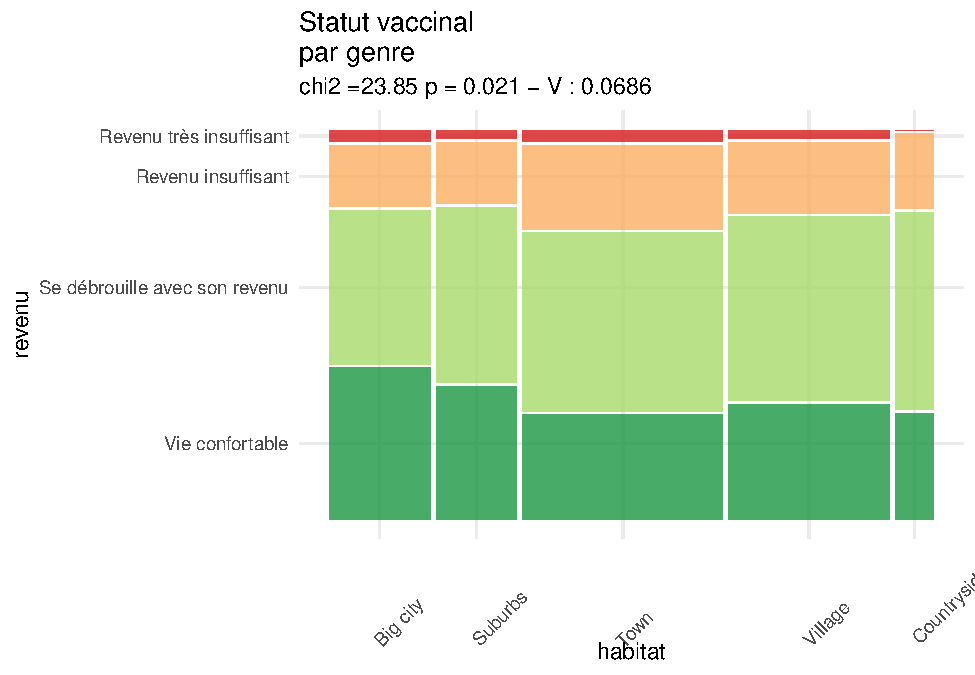
\includegraphics{bookdown-demo_files/figure-latex/0428-1.pdf}

\hypertarget{les-chi2s-partiel-et-des-cartes-de-chaleur.}{%
\subsubsection{les chi2s partiel et des cartes de chaleur.}\label{les-chi2s-partiel-et-des-cartes-de-chaleur.}}

Une carte de chaleur représente une grandeur par un gradient de couleur pour chaque cellule définie par des variable x et y.

Faisons un premier essai pour représenter les effectifs, plutôt qu'avoir un tableau de nombres on va obtenir un tableau de couleurs.

L'arbre qui apparait en ligne et en colonne correspond au résultat d'une classification hiérarchique que nous développons dans le chapitre X.

\begin{Shaded}
\begin{Highlighting}[]
\KeywordTok{library}\NormalTok{(pheatmap)}
\KeywordTok{library}\NormalTok{(viridis)}

\NormalTok{table2<-}\KeywordTok{as.data.frame}\NormalTok{(t) }\OperatorTok
\StringTok{  }\KeywordTok{pivot_wider}\NormalTok{(}\DataTypeTok{names_from =}\NormalTok{ Var1, }\DataTypeTok{values_from =}\NormalTok{ Freq) }\OperatorTok
\StringTok{  }\KeywordTok{column_to_rownames}\NormalTok{( }\DataTypeTok{var =} \StringTok{"Var2"}\NormalTok{)}
\KeywordTok{pheatmap}\NormalTok{(table2 , }\DataTypeTok{color =} \KeywordTok{rocket}\NormalTok{(}\DecValTok{10}\NormalTok{,}\DataTypeTok{direction =}\OperatorTok{-}\DecValTok{1}\NormalTok{))}
\end{Highlighting}
\end{Shaded}

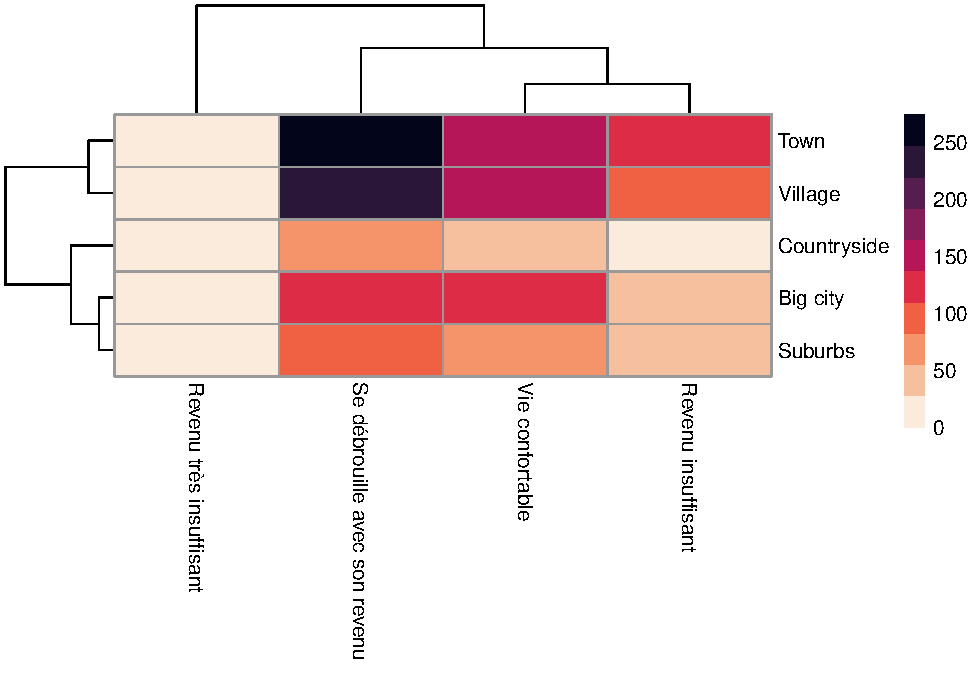
\includegraphics{bookdown-demo_files/figure-latex/0429-1.pdf}

On utilise la même technique mais en représenant une grandeur différentes : les tests du chi2 partiels, pour apprécier les sous ou les sur-représentation.

\begin{Shaded}
\begin{Highlighting}[]
\KeywordTok{library}\NormalTok{(RColorBrewer)}
\NormalTok{chi2df<-}\StringTok{ }\KeywordTok{as.data.frame}\NormalTok{(chi2}\OperatorTok{$}\NormalTok{stdres)}

\NormalTok{table2<-chi2df }\OperatorTok\StringTok{ }
\StringTok{  }\KeywordTok{pivot_wider}\NormalTok{(}\DataTypeTok{names_from =}\NormalTok{ Var1, }\DataTypeTok{values_from =}\NormalTok{ Freq) }\OperatorTok
\StringTok{  }\KeywordTok{column_to_rownames}\NormalTok{( }\DataTypeTok{var =} \StringTok{"Var2"}\NormalTok{)}
\KeywordTok{pheatmap}\NormalTok{(table2 , }\DataTypeTok{color =} \KeywordTok{brewer.pal}\NormalTok{(}\DataTypeTok{n =} \DecValTok{9}\NormalTok{, }\DataTypeTok{name =} \StringTok{"RdBu"}\NormalTok{))}
\end{Highlighting}
\end{Shaded}

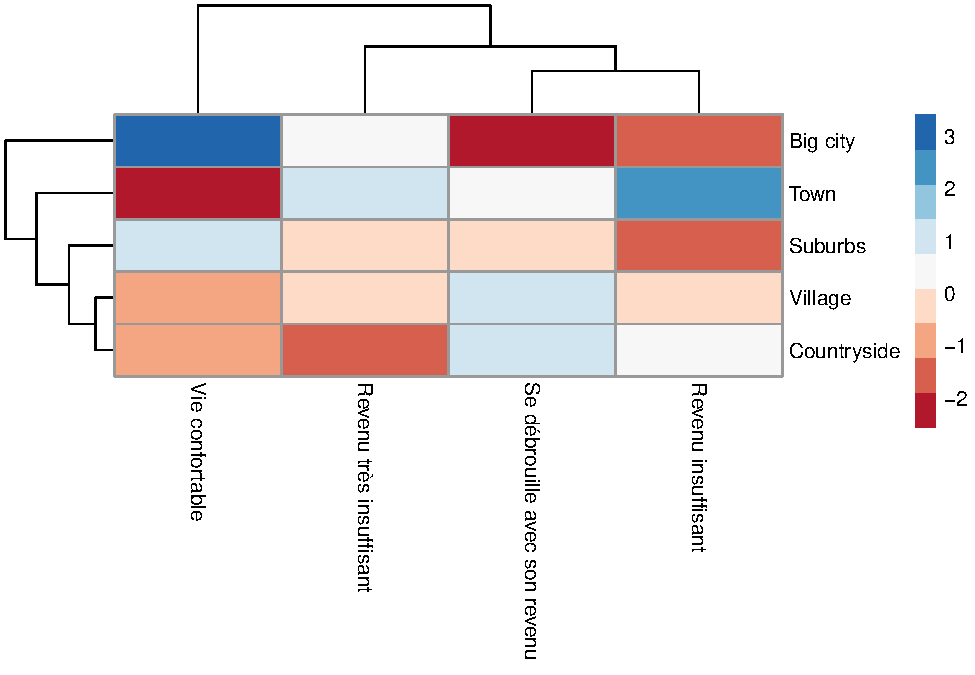
\includegraphics{bookdown-demo_files/figure-latex/0430-1.pdf}

\hypertarget{les-treemaps-cest-merveilleux}{%
\subsubsection{Les treemaps, c'est merveilleux}\label{les-treemaps-cest-merveilleux}}

D'autre graphiques et des emboitements

\begin{Shaded}
\begin{Highlighting}[]
\KeywordTok{library}\NormalTok{(treemapify)}
\NormalTok{tree1<-df }\OperatorTok\StringTok{ }\KeywordTok{mutate}\NormalTok{(}\DataTypeTok{n=}\DecValTok{1}\NormalTok{)}\OperatorTok\KeywordTok{group_by}\NormalTok{(cntry,genre,habitat) }\OperatorTok\StringTok{ }\KeywordTok{summarize}\NormalTok{(}\DataTypeTok{n=}\KeywordTok{sum}\NormalTok{(n),}\DataTypeTok{mean=}\KeywordTok{mean}\NormalTok{(trust_interpersonnel, }\DataTypeTok{na.rm=}\OtherTok{TRUE}\NormalTok{))}

\NormalTok{g10 <-}\StringTok{ }\KeywordTok{ggplot}\NormalTok{(tree1, }\KeywordTok{aes}\NormalTok{(}\DataTypeTok{area =}\NormalTok{ n, }\DataTypeTok{fill=}\NormalTok{genre,}\DataTypeTok{subgroup=}\NormalTok{cntry)) }\OperatorTok{+}
\StringTok{  }\KeywordTok{geom_treemap}\NormalTok{() }\OperatorTok{+}\StringTok{   }
\StringTok{  }\KeywordTok{geom_treemap_text}\NormalTok{(}\KeywordTok{aes}\NormalTok{(}\DataTypeTok{label=}\NormalTok{habitat),}\DataTypeTok{colour =} \StringTok{"white"}\NormalTok{, }\DataTypeTok{place =} \StringTok{"centre"}\NormalTok{,}\DataTypeTok{grow =} \OtherTok{FALSE}\NormalTok{)}\OperatorTok{+}
\StringTok{      }\KeywordTok{geom_treemap_subgroup_text}\NormalTok{(}\DataTypeTok{color=}\StringTok{"white"}\NormalTok{,}\DataTypeTok{grow =} \OtherTok{FALSE}\NormalTok{)}\OperatorTok{+}
\StringTok{  }\KeywordTok{geom_treemap_subgroup_border}\NormalTok{()}
\NormalTok{g10}
\end{Highlighting}
\end{Shaded}

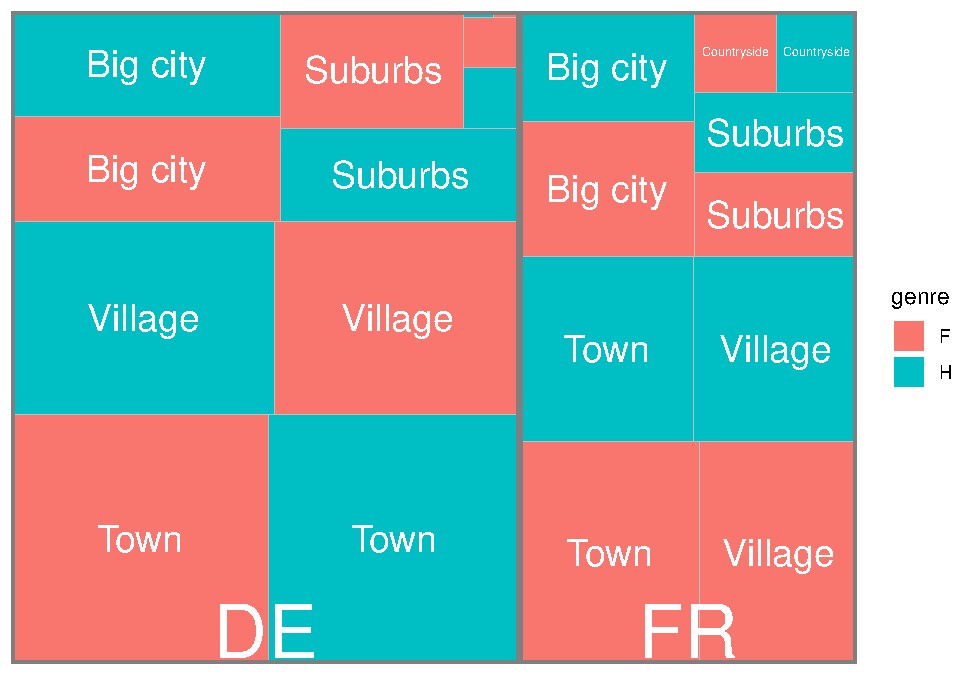
\includegraphics{bookdown-demo_files/figure-latex/0431-1.pdf}

\hypertarget{analyse-graphique-multivariuxe9e}{%
\chapter{Analyse graphique multivariée}\label{analyse-graphique-multivariuxe9e}}

Dans ce chapitre, on généralise à des ensembles de variables.

\hypertarget{la-confiance-institutionnelle-en-duxe9tail}{%
\section{La confiance institutionnelle, en détail}\label{la-confiance-institutionnelle-en-duxe9tail}}

On veut reprénter 6 variables, correspondant à 5 types d'habitats et 2 pays.

\begin{Shaded}
\begin{Highlighting}[]
\NormalTok{df<-}\KeywordTok{readRDS}\NormalTok{(}\StringTok{"./data/dfTrust.rds)"}\NormalTok{)}


\NormalTok{rad<-df }\OperatorTok\StringTok{ }
\StringTok{  }\KeywordTok{group_by}\NormalTok{ (habitat,cntry) }\OperatorTok\StringTok{ }
\StringTok{  }\KeywordTok{summarize}\NormalTok{(}\DataTypeTok{Partis=}\KeywordTok{mean}\NormalTok{(Partis, }\DataTypeTok{na.rm=}\OtherTok{TRUE}\NormalTok{),}
  \DataTypeTok{Parlement=}\KeywordTok{mean}\NormalTok{(Parlement, }\DataTypeTok{na.rm=}\OtherTok{TRUE}\NormalTok{),}
  \DataTypeTok{Politiques=}\KeywordTok{mean}\NormalTok{(Politiques, }\DataTypeTok{na.rm=}\OtherTok{TRUE}\NormalTok{),}
  \DataTypeTok{Police=}\KeywordTok{mean}\NormalTok{(Police, }\DataTypeTok{na.rm=}\OtherTok{TRUE}\NormalTok{),}
  \DataTypeTok{Justice=}\KeywordTok{mean}\NormalTok{(Justice, }\DataTypeTok{na.rm=}\OtherTok{TRUE}\NormalTok{),}
  \DataTypeTok{NationsUnies=}\KeywordTok{mean}\NormalTok{(NationsUnies, }\DataTypeTok{na.rm=}\OtherTok{TRUE}\NormalTok{),}
  \DataTypeTok{ParlementEurop=}\KeywordTok{mean}\NormalTok{(ParlementEurop, }\DataTypeTok{na.rm=}\OtherTok{TRUE}\NormalTok{)) }\OperatorTok\StringTok{ }
\StringTok{  }\KeywordTok{filter}\NormalTok{(}\OperatorTok{!}\KeywordTok{is.na}\NormalTok{(habitat)) }\OperatorTok
\StringTok{  }\KeywordTok{gather}\NormalTok{(variable, value, }\OperatorTok{-}\NormalTok{habitat, }\OperatorTok{-}\NormalTok{cntry)}

\KeywordTok{ggplot}\NormalTok{(rad, }\KeywordTok{aes}\NormalTok{(}\DataTypeTok{x=}\KeywordTok{reorder}\NormalTok{(variable, value),}\DataTypeTok{y=}\NormalTok{value, }\DataTypeTok{group=}\NormalTok{habitat))}\OperatorTok{+}
\StringTok{  }\KeywordTok{geom_line}\NormalTok{(}\KeywordTok{aes}\NormalTok{(}\DataTypeTok{color=}\NormalTok{habitat), }\DataTypeTok{size=}\DecValTok{2}\NormalTok{)}\OperatorTok{+}
\StringTok{  }\KeywordTok{facet_grid}\NormalTok{(.}\OperatorTok{~}\NormalTok{cntry) }\OperatorTok{+}\KeywordTok{coord_flip}\NormalTok{()}\OperatorTok{+}
\StringTok{  }\KeywordTok{scale_color_brewer}\NormalTok{(}\DataTypeTok{type=}\StringTok{"div"}\NormalTok{,}\DataTypeTok{palette=}\DecValTok{3}\NormalTok{)}\OperatorTok{+}\KeywordTok{labs}\NormalTok{(}\DataTypeTok{title=} \StringTok{"Les éléments de la confiance institutionnelle"}\NormalTok{, }\DataTypeTok{caption=}\StringTok{"ESS2002-2018"}\NormalTok{,}\DataTypeTok{y=} \StringTok{"confiance (de 1 à 10)"}\NormalTok{,}\DataTypeTok{x=}\StringTok{"institutions"}\NormalTok{) }
\end{Highlighting}
\end{Shaded}

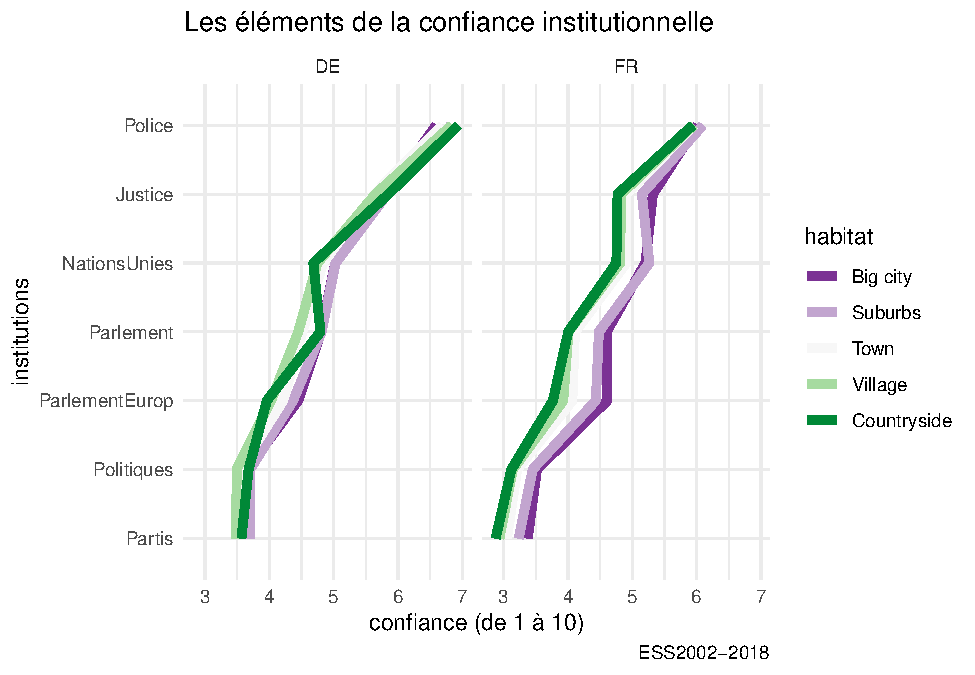
\includegraphics{bookdown-demo_files/figure-latex/0501-1.pdf}

Une autre variante qui donne l'évolution de l'évolution de les éléments de la confiance institutionnelle

\begin{Shaded}
\begin{Highlighting}[]
\NormalTok{rad<-df }\OperatorTok\StringTok{ }
\StringTok{  }\KeywordTok{group_by}\NormalTok{ (Year,cntry) }\OperatorTok\StringTok{ }
\StringTok{  }\KeywordTok{summarize}\NormalTok{(}\DataTypeTok{Partis=}\KeywordTok{mean}\NormalTok{(Partis, }\DataTypeTok{na.rm=}\OtherTok{TRUE}\NormalTok{),}
  \DataTypeTok{Parlement=}\KeywordTok{mean}\NormalTok{(Parlement, }\DataTypeTok{na.rm=}\OtherTok{TRUE}\NormalTok{),}
  \DataTypeTok{Politiques=}\KeywordTok{mean}\NormalTok{(Politiques, }\DataTypeTok{na.rm=}\OtherTok{TRUE}\NormalTok{),}
  \DataTypeTok{Police=}\KeywordTok{mean}\NormalTok{(Police, }\DataTypeTok{na.rm=}\OtherTok{TRUE}\NormalTok{),}
  \DataTypeTok{Justice=}\KeywordTok{mean}\NormalTok{(Justice, }\DataTypeTok{na.rm=}\OtherTok{TRUE}\NormalTok{),}
  \DataTypeTok{NationsUnies=}\KeywordTok{mean}\NormalTok{(NationsUnies, }\DataTypeTok{na.rm=}\OtherTok{TRUE}\NormalTok{),}
  \DataTypeTok{ParlementEurop=}\KeywordTok{mean}\NormalTok{(ParlementEurop, }\DataTypeTok{na.rm=}\OtherTok{TRUE}\NormalTok{)) }\OperatorTok\StringTok{ }
\StringTok{  }\KeywordTok{gather}\NormalTok{(variable, value, }\OperatorTok{-}\NormalTok{Year, }\OperatorTok{-}\NormalTok{cntry)}

\KeywordTok{ggplot}\NormalTok{(rad, }\KeywordTok{aes}\NormalTok{(}\DataTypeTok{x=}\NormalTok{Year,}\DataTypeTok{y=}\NormalTok{value, }\DataTypeTok{group=}\NormalTok{variable))}\OperatorTok{+}
\StringTok{  }\KeywordTok{geom_line}\NormalTok{(}\KeywordTok{aes}\NormalTok{(}\DataTypeTok{color=}\NormalTok{variable), }\DataTypeTok{size=}\FloatTok{1.2}\NormalTok{)}\OperatorTok{+}
\StringTok{  }\KeywordTok{facet_wrap}\NormalTok{(.}\OperatorTok{~}\NormalTok{cntry, }\DataTypeTok{nrow=}\DecValTok{1}\NormalTok{) }\OperatorTok{+}
\StringTok{  }\KeywordTok{scale_color_brewer}\NormalTok{(}\DataTypeTok{palette=}\StringTok{"Spectral"}\NormalTok{)}\OperatorTok{+}\KeywordTok{labs}\NormalTok{(}\DataTypeTok{title=} \StringTok{"Les éléments de la confiance institutionnelle"}\NormalTok{, }\DataTypeTok{caption=}\StringTok{"ESS2002-2018"}\NormalTok{,}\DataTypeTok{y=} \StringTok{"confiance (de 1 à 10)"}\NormalTok{,}\DataTypeTok{x=}\StringTok{"institutions"}\NormalTok{) }
\end{Highlighting}
\end{Shaded}

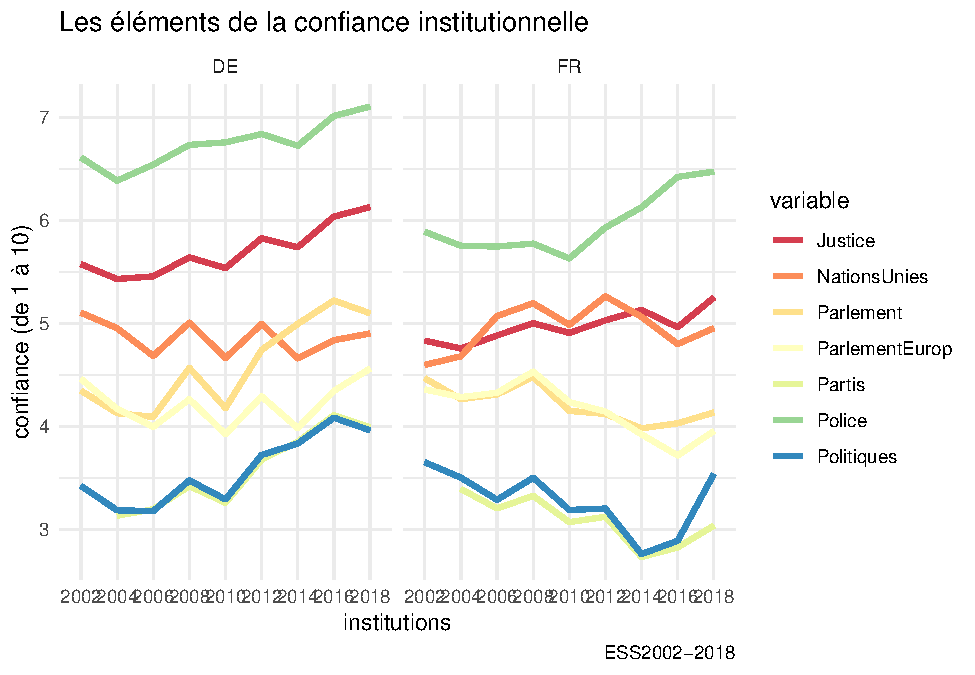
\includegraphics{bookdown-demo_files/figure-latex/0503-1.pdf}

La différence entre les deux pays est claire, la rupture est accusée plus fortement en France qu'en Allemagne. L'explication n'est sans doute pas culturelle mais démographique, un coup d'oeil à la carte des densité permet de comprendre mieux : \url{https://www.populationdata.net/cartes/allemagne-france-densite-de-population-2011/}.

On pourra tenté un graphe en radar. Mais il n'est pas si convaincant.

\begin{Shaded}
\begin{Highlighting}[]
\KeywordTok{library}\NormalTok{(fmsb)}

\NormalTok{rad<-df }\OperatorTok\StringTok{ }\KeywordTok{filter}\NormalTok{(cntry}\OperatorTok{==}\StringTok{"FR"}\NormalTok{) }\OperatorTok
\StringTok{  }\KeywordTok{group_by}\NormalTok{ (habitat) }\OperatorTok
\StringTok{  }\KeywordTok{summarize}\NormalTok{(}\DataTypeTok{Partis=}\KeywordTok{mean}\NormalTok{(Partis, }\DataTypeTok{na.rm=}\OtherTok{TRUE}\NormalTok{),}
  \DataTypeTok{Parlement=}\KeywordTok{mean}\NormalTok{(Parlement, }\DataTypeTok{na.rm=}\OtherTok{TRUE}\NormalTok{),}
  \DataTypeTok{Politiques=}\KeywordTok{mean}\NormalTok{(Politiques, }\DataTypeTok{na.rm=}\OtherTok{TRUE}\NormalTok{),}
  \DataTypeTok{Police=}\KeywordTok{mean}\NormalTok{(Police, }\DataTypeTok{na.rm=}\OtherTok{TRUE}\NormalTok{),}
  \DataTypeTok{Justice=}\KeywordTok{mean}\NormalTok{(Justice, }\DataTypeTok{na.rm=}\OtherTok{TRUE}\NormalTok{),}
  \DataTypeTok{NationsUnies=}\KeywordTok{mean}\NormalTok{(NationsUnies, }\DataTypeTok{na.rm=}\OtherTok{TRUE}\NormalTok{),}
  \DataTypeTok{ParlementEurop=}\KeywordTok{mean}\NormalTok{(ParlementEurop, }\DataTypeTok{na.rm=}\OtherTok{TRUE}\NormalTok{)) }\OperatorTok\StringTok{ }
\StringTok{  }\KeywordTok{filter}\NormalTok{(}\OperatorTok{!}\KeywordTok{is.na}\NormalTok{(habitat)) }\OperatorTok\StringTok{ }
\StringTok{  }\NormalTok{dplyr}\OperatorTok{::}\KeywordTok{select}\NormalTok{(}\OperatorTok{-}\NormalTok{habitat)}

\CommentTok{#on doit indiquer les valeurs minimale et maximale - la fonction rep permet de repeter (ici 7 fois pour les 7 variables/col)}
\NormalTok{data <-}\StringTok{ }\KeywordTok{rbind}\NormalTok{(}\KeywordTok{rep}\NormalTok{(}\DecValTok{7}\NormalTok{,}\DecValTok{7}\NormalTok{) , }\KeywordTok{rep}\NormalTok{(}\DecValTok{3}\NormalTok{,}\DecValTok{7}\NormalTok{) , rad)}
\CommentTok{#l'autre method c'est ce choisir maxmin=FALSE}

\CommentTok{#rownames(rad) <- c("big city", "suburbs" ,"town","village", "countryside")}
\KeywordTok{radarchart}\NormalTok{(rad, }\DataTypeTok{axistype=}\DecValTok{0}\NormalTok{, }\DataTypeTok{seg=}\DecValTok{4}\NormalTok{, }\DataTypeTok{title=}\StringTok{"Moyenne par institution"}\NormalTok{, }\DataTypeTok{maxmin=}\OtherTok{FALSE}\NormalTok{)}
\KeywordTok{legend}\NormalTok{(}\DataTypeTok{x=}\FloatTok{0.7}\NormalTok{, }\DataTypeTok{y=}\DecValTok{1}\NormalTok{, }\DataTypeTok{legend =} \KeywordTok{rownames}\NormalTok{(rad), }\DataTypeTok{bty =} \StringTok{"n"}\NormalTok{,}\DataTypeTok{text.col =} \StringTok{"grey"}\NormalTok{, }\DataTypeTok{cex=}\FloatTok{1.2}\NormalTok{, }\DataTypeTok{pt.cex=}\DecValTok{3}\NormalTok{)}
\end{Highlighting}
\end{Shaded}

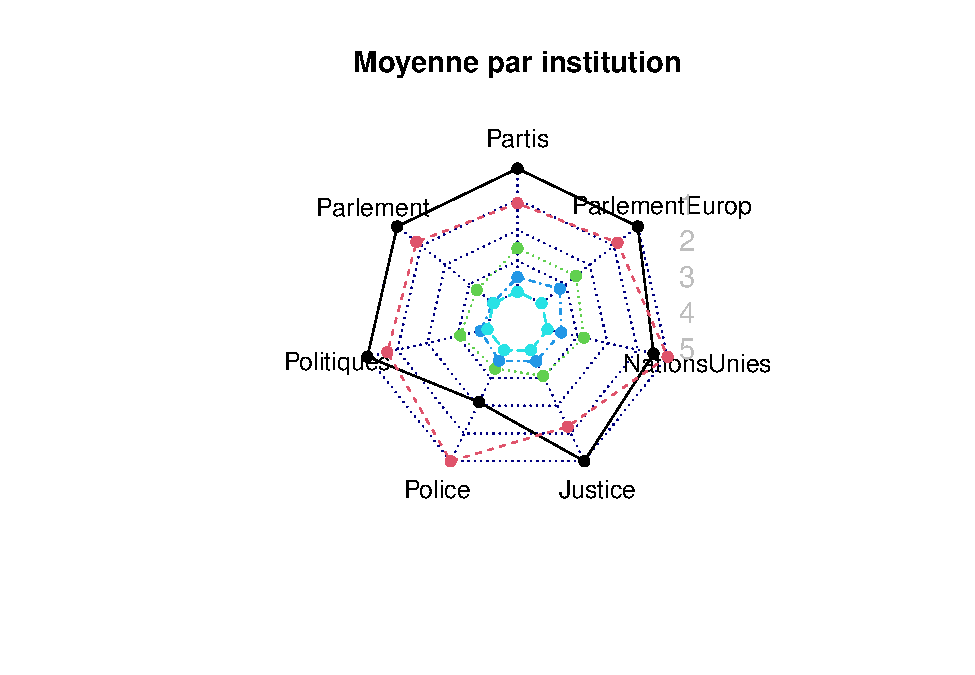
\includegraphics{bookdown-demo_files/figure-latex/0504-1.pdf}

\hypertarget{table-de-corruxe9lation}{%
\section{Table de corrélation}\label{table-de-corruxe9lation}}

Comparer les moyennes est une chose, on souhaiter en plus savoir quelle structure de corrélation les caractérisent. Rien de plus simple

\begin{Shaded}
\begin{Highlighting}[]
\KeywordTok{library}\NormalTok{(ggcorrplot)}
\NormalTok{df<-}\KeywordTok{readRDS}\NormalTok{(}\StringTok{"./data/dfTrust.rds)"}\NormalTok{)}\OperatorTok\KeywordTok{filter}\NormalTok{(Year}\OperatorTok{==}\DecValTok{2018}\NormalTok{)}

\NormalTok{foo<-df }\OperatorTok\StringTok{ }\NormalTok{dplyr}\OperatorTok{::}\KeywordTok{select}\NormalTok{(NationsUnies,ParlementEurop, Parlement, Justice, Police, Politiques, Partis) }\OperatorTok\StringTok{ }
\StringTok{  }\KeywordTok{drop_na}\NormalTok{()}
\NormalTok{r<-}\KeywordTok{cor}\NormalTok{(foo)}

\KeywordTok{ggcorrplot}\NormalTok{(r, }\DataTypeTok{hc.order =} \OtherTok{TRUE}\NormalTok{, }\DataTypeTok{type =} \StringTok{"lower"}\NormalTok{,}
   \DataTypeTok{lab =} \OtherTok{TRUE}\NormalTok{)}
\end{Highlighting}
\end{Shaded}

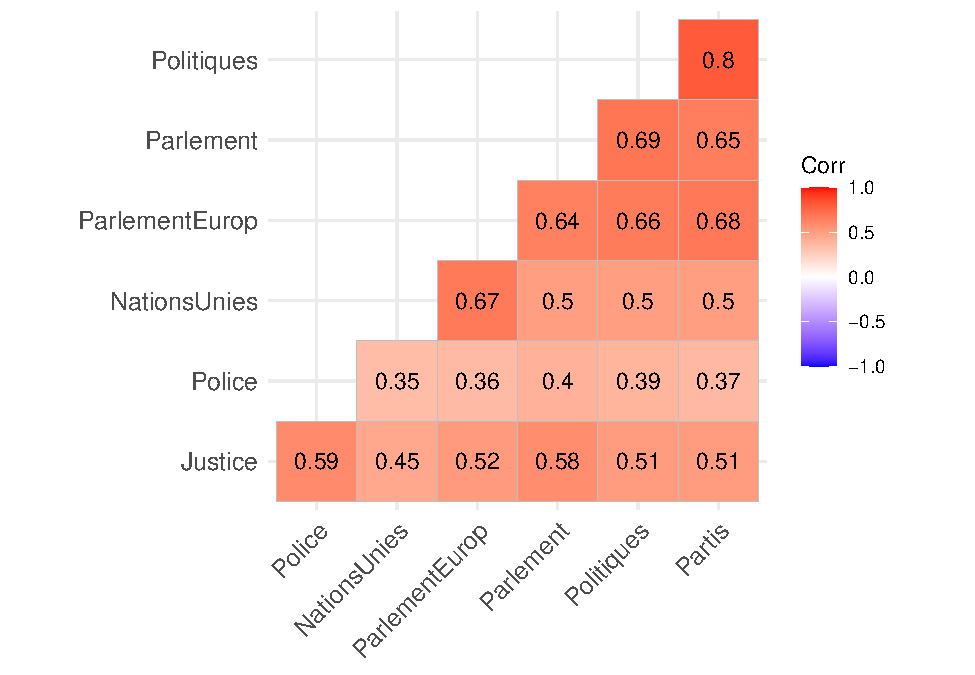
\includegraphics{bookdown-demo_files/figure-latex/0505-1.pdf}

\begin{Shaded}
\begin{Highlighting}[]
\NormalTok{g<-}\KeywordTok{paste0}\NormalTok{(}\StringTok{"./plot/g1"}\NormalTok{,}\StringTok{".jpg"}\NormalTok{)}
\KeywordTok{ggsave}\NormalTok{(g,}\DataTypeTok{plot=}\KeywordTok{last_plot}\NormalTok{(), }\DataTypeTok{width =} \DecValTok{27}\NormalTok{, }\DataTypeTok{height =} \DecValTok{19}\NormalTok{, }\DataTypeTok{units =} \StringTok{"cm"}\NormalTok{)}
\end{Highlighting}
\end{Shaded}

\hypertarget{un-cas-plus-complexe-pruxe9sidentielle2020}{%
\section{Un cas plus complexe : présidentielle2020}\label{un-cas-plus-complexe-pruxe9sidentielle2020}}

Nsppolls cumulent les sondages publiés des grands instituts. On utilise ces données , ainsi qu'une boucle, pour explorer différents paramètre d'un modèle de lissage.

Le but : mieux percevoir les tendance par une sorte de méta-analyse des différents sondages :

\hypertarget{une-boucle-pour-produire-de-multiple-graphe-en-variant-un-paramuxe8tre}{%
\section{une boucle pour produire de multiple graphe en variant un paramètre}\label{une-boucle-pour-produire-de-multiple-graphe-en-variant-un-paramuxe8tre}}

\begin{Shaded}
\begin{Highlighting}[]
\KeywordTok{library}\NormalTok{(lubridate)}
\NormalTok{alph<-.}\DecValTok{5}

\ControlFlowTok{for}\NormalTok{ (alph }\ControlFlowTok{in} \KeywordTok{seq}\NormalTok{(}\DataTypeTok{from=}\DecValTok{0}\NormalTok{, }\DataTypeTok{to=} \DecValTok{1}\NormalTok{, }\DataTypeTok{by=}\NormalTok{.}\DecValTok{05}\NormalTok{))\{}
\NormalTok{df_pol <-}\StringTok{ }\KeywordTok{read_delim}\NormalTok{(}\StringTok{"https://raw.githubusercontent.com/nsppolls/nsppolls/master/presidentielle.csv"}\NormalTok{, }
                     \DataTypeTok{delim =} \StringTok{","}\NormalTok{, }\DataTypeTok{escape_double =} \OtherTok{FALSE}\NormalTok{, }\DataTypeTok{trim_ws =} \OtherTok{TRUE}\NormalTok{)}\OperatorTok
\StringTok{  }\KeywordTok{filter}\NormalTok{(tour}\OperatorTok{==}\StringTok{"Premier tour"}\NormalTok{) }\OperatorTok\KeywordTok{filter}\NormalTok{(candidat}\OperatorTok{==}\StringTok{"Eric Zemmour"}\OperatorTok{|}
\StringTok{                                           }\NormalTok{candidat}\OperatorTok{==}\StringTok{ "Marine Le Pen"}\OperatorTok{|}
\StringTok{                                           }\NormalTok{candidat}\OperatorTok{==}\StringTok{ "Emmanuel Macron"}\OperatorTok{|}
\StringTok{                                           }\NormalTok{candidat}\OperatorTok{==}\StringTok{ "Jean-Luc Mélenchon"}\OperatorTok{|}
\StringTok{                                           }\NormalTok{candidat}\OperatorTok{==}\StringTok{ "Yannick Jadot"}\OperatorTok{|}
\StringTok{                                           }\NormalTok{candidat}\OperatorTok{==}\StringTok{ "Valérie Pécresse"}\OperatorTok{|}\StringTok{ }
\StringTok{                                           }\NormalTok{candidat}\OperatorTok{==}\StringTok{"Fabien Roussel"}\OperatorTok{|}
\StringTok{                                           }\NormalTok{candidat}\OperatorTok{==}\StringTok{"Anne Hidalgo"}\NormalTok{) }\OperatorTok
\StringTok{  }\KeywordTok{filter}\NormalTok{(fin_enquete}\OperatorTok{>}\KeywordTok{ymd}\NormalTok{(}\StringTok{"2022-01-09"}\NormalTok{)) }\CommentTok{# on commence en septembre , octobre est-il meilleur ?}


\KeywordTok{table}\NormalTok{(df_pol}\OperatorTok{$}\NormalTok{candidat)}
\NormalTok{SensiP1<-}\KeywordTok{c}\NormalTok{(}\StringTok{"pink"}\NormalTok{, }\StringTok{"orange"}\NormalTok{, }\StringTok{"gray20"}\NormalTok{, }\StringTok{"red"}\NormalTok{,}\StringTok{"firebrick"}\NormalTok{, }\StringTok{"Royalblue"}\NormalTok{, }\StringTok{" skyblue"}\NormalTok{, }\StringTok{"Chartreuse"}\NormalTok{)}

\KeywordTok{ggplot}\NormalTok{(df_pol, }\KeywordTok{aes}\NormalTok{(}\DataTypeTok{y=}\NormalTok{intentions, }\DataTypeTok{x=}\NormalTok{fin_enquete))}\OperatorTok{+}
\StringTok{  }\KeywordTok{geom_point}\NormalTok{(}\KeywordTok{aes}\NormalTok{(}\DataTypeTok{color=}\NormalTok{candidat), }\DataTypeTok{size=}\NormalTok{.}\DecValTok{5}\NormalTok{, }\DataTypeTok{alpha=}\DecValTok{1}\OperatorTok{-}\NormalTok{alph)}\OperatorTok{+}
\StringTok{  }\KeywordTok{geom_smooth}\NormalTok{(}\DataTypeTok{span =}\NormalTok{ alph, }\KeywordTok{aes}\NormalTok{(}\DataTypeTok{col=}\NormalTok{candidat,}\DataTypeTok{fill=}\NormalTok{candidat), }\DataTypeTok{alpha=}\FloatTok{0.2}\NormalTok{)}\OperatorTok{+}
\StringTok{  }\KeywordTok{scale_color_manual}\NormalTok{(}\DataTypeTok{values=}\NormalTok{SensiP1)}\OperatorTok{+}\StringTok{  }
\StringTok{  }\KeywordTok{scale_fill_manual}\NormalTok{(}\DataTypeTok{values=}\NormalTok{SensiP1)}\OperatorTok{+}\StringTok{ }
\StringTok{  }\KeywordTok{labs}\NormalTok{(}\DataTypeTok{title=} \StringTok{"Evolution des intentions de vote #présidentielle2022 1er tour"}\NormalTok{,}
       \DataTypeTok{subtitle =}\KeywordTok{paste}\NormalTok{(}\StringTok{"Lissage méthode loess. alpha="}\NormalTok{,alph, }\StringTok{" - ci=95%"}\NormalTok{),}
       \DataTypeTok{caption =} \StringTok{"data @nsppolls viz @benavent"}\NormalTok{,}
       \DataTypeTok{x=}\OtherTok{NULL}\NormalTok{)}\OperatorTok{+}\KeywordTok{theme_minimal}\NormalTok{()}\OperatorTok{+}\KeywordTok{scale_x_date}\NormalTok{(}\DataTypeTok{date_breaks =} \StringTok{"1 month"}\NormalTok{, }\DataTypeTok{date_minor_breaks =} \StringTok{"1 week"}\NormalTok{,}
             \DataTypeTok{date_labels =} \StringTok{"%B"}\NormalTok{)}

\NormalTok{sondage_nsppolls<-}\KeywordTok{paste0}\NormalTok{(}\StringTok{"./nsppolls/sondage_nsppolls"}\NormalTok{, alph}\OperatorTok{*}\DecValTok{20}\NormalTok{, }\StringTok{".jpg"}\NormalTok{)}
\KeywordTok{ggsave}\NormalTok{(sondage_nsppolls,}\DataTypeTok{plot=}\KeywordTok{last_plot}\NormalTok{(), }\DataTypeTok{width =} \DecValTok{27}\NormalTok{, }\DataTypeTok{height =} \DecValTok{19}\NormalTok{, }\DataTypeTok{units =} \StringTok{"cm"}\NormalTok{)}

\NormalTok{\}}


\NormalTok{n<-df_pol}\OperatorTok
\StringTok{  }\KeywordTok{mutate}\NormalTok{(}\DataTypeTok{n=}\DecValTok{1}\NormalTok{)}\OperatorTok
\StringTok{  }\KeywordTok{group_by}\NormalTok{(id)}\OperatorTok\KeywordTok{summarise}\NormalTok{(}\DataTypeTok{n=}\KeywordTok{sum}\NormalTok{(n))}
\CommentTok{#nombre de sondage}
\NormalTok{n<-}\KeywordTok{nrow}\NormalTok{(n)}
\end{Highlighting}
\end{Shaded}

Pour créer le gif on emplie magick. On a pris soin de sauvegarder les graphes dans un répertoire propre, ça facilite la lecture en boucle et la fabrication du gif.

\begin{Shaded}
\begin{Highlighting}[]
\KeywordTok{library}\NormalTok{(magick)}

\CommentTok{#gif                                                     }

\CommentTok{#on constitue une liste des noms des fichier *.jpg que l'on veut associer                                                     }
\NormalTok{frames <-}\StringTok{ }\KeywordTok{paste0}\NormalTok{(}\StringTok{"./nsppolls/"}\NormalTok{,}\StringTok{"sondage_nsppolls"}\NormalTok{, }\DecValTok{0}\OperatorTok{:}\DecValTok{20}\NormalTok{,}\StringTok{".jpg"}\NormalTok{)}

\CommentTok{#on lit et on stoke dans m les images}
\NormalTok{m <-}\StringTok{ }\KeywordTok{image_read}\NormalTok{(frames)}

\CommentTok{#on fabrique et on sauvergarde le gif}
\NormalTok{m <-}\StringTok{ }\KeywordTok{image_animate}\NormalTok{(m, }\DataTypeTok{fps=}\DecValTok{1}\NormalTok{)}
\KeywordTok{image_write}\NormalTok{(m, }\StringTok{"./plot/sondages_lissage.gif"}\NormalTok{)}
\end{Highlighting}
\end{Shaded}

\hypertarget{effet-sondeur}{%
\subsection{effet sondeur}\label{effet-sondeur}}

pour anticiper sur le chapitre suivant

\begin{Shaded}
\begin{Highlighting}[]
\NormalTok{foo<-df_pol}\OperatorTok
\StringTok{  }\NormalTok{dplyr}\OperatorTok{::}\KeywordTok{select}\NormalTok{(candidat, intentions, fin_enquete, echantillon,nom_institut)}\OperatorTok
\StringTok{  }\KeywordTok{group_by}\NormalTok{(nom_institut, candidat)}\OperatorTok
\StringTok{  }\KeywordTok{summarise}\NormalTok{(}\DataTypeTok{moy=}\KeywordTok{mean}\NormalTok{(intentions, }\DataTypeTok{na.rm=}\OtherTok{TRUE}\NormalTok{),}
            \DataTypeTok{std=}\KeywordTok{sd}\NormalTok{(intentions, }\DataTypeTok{na.rm=}\OtherTok{TRUE}\NormalTok{))}


\NormalTok{SensiP2<-}\KeywordTok{c}\NormalTok{(}\StringTok{"gray90"}\NormalTok{,}\StringTok{"gray20"}\NormalTok{, }\StringTok{"Royalblue"}\NormalTok{, }\StringTok{"skyblue"}\NormalTok{, }\StringTok{"orange"}\NormalTok{, }\StringTok{"yellow"}\NormalTok{, }\StringTok{"pink"}\NormalTok{, }\StringTok{"firebrick"}\NormalTok{, }\StringTok{"green"}\NormalTok{)}


\NormalTok{g<-}\KeywordTok{ggplot}\NormalTok{(foo,}\KeywordTok{aes}\NormalTok{(}\DataTypeTok{x=}\NormalTok{candidat,}\DataTypeTok{y=}\NormalTok{moy))}\OperatorTok{+}
\StringTok{  }\KeywordTok{geom_segment}\NormalTok{(}\KeywordTok{aes}\NormalTok{(}\DataTypeTok{x =}\NormalTok{ candidat, }
                   \DataTypeTok{y =} \OperatorTok{-}\NormalTok{std}\OperatorTok{+}\NormalTok{moy, }
                   \DataTypeTok{xend =}\NormalTok{ candidat, }
                   \DataTypeTok{yend =}\NormalTok{ std}\OperatorTok{+}\NormalTok{moy, }
                   \DataTypeTok{color =}\NormalTok{ nom_institut), }\DataTypeTok{size=}\FloatTok{1.2}\NormalTok{)}\OperatorTok{+}
\StringTok{    }\KeywordTok{geom_point}\NormalTok{(}\KeywordTok{aes}\NormalTok{(}\DataTypeTok{color=}\NormalTok{nom_institut), }\DataTypeTok{size=}\DecValTok{2}\NormalTok{)}\OperatorTok{+}
\StringTok{  }\KeywordTok{scale_color_manual}\NormalTok{(}\DataTypeTok{values =}\NormalTok{ SensiP2)}\OperatorTok{+}
\StringTok{  }\KeywordTok{theme_minimal}\NormalTok{()}\OperatorTok{+}
\StringTok{  }\KeywordTok{coord_flip}\NormalTok{()}
\NormalTok{g}
\end{Highlighting}
\end{Shaded}

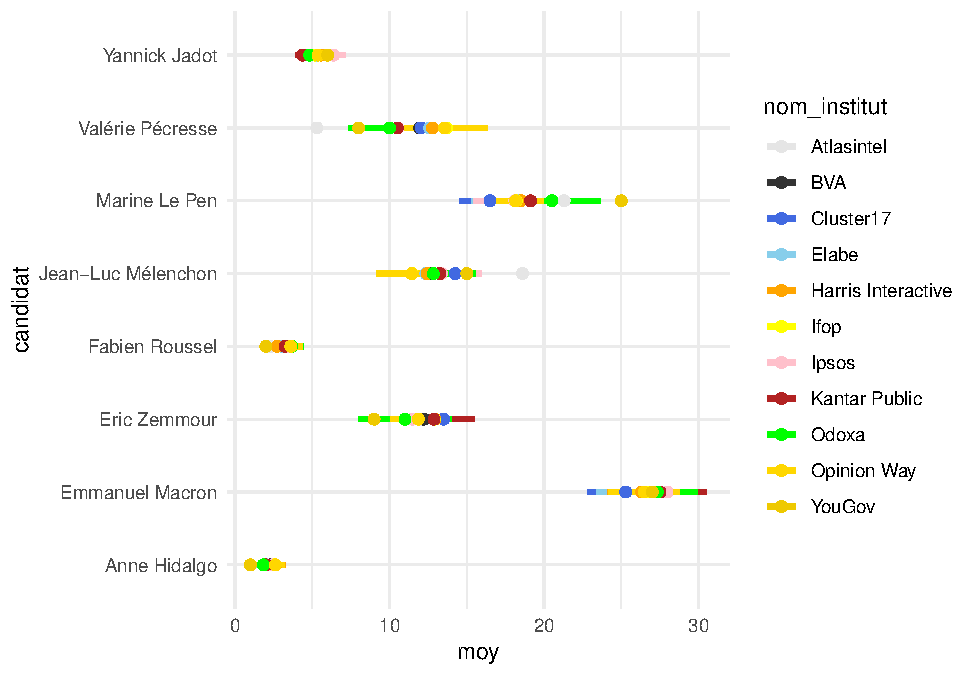
\includegraphics{bookdown-demo_files/figure-latex/0510-1.pdf}

\hypertarget{moduxe9liser-le-biais-du-sondeur}{%
\section{Modéliser le biais du sondeur}\label{moduxe9liser-le-biais-du-sondeur}}

\url{http://www.stat.yale.edu/Courses/1997-98/101/anovareg.htm}

\begin{Shaded}
\begin{Highlighting}[]
\NormalTok{df_pol}\OperatorTok{$}\NormalTok{tps<-}\DecValTok{2}
\NormalTok{df_pol}\OperatorTok{$}\NormalTok{tps[df_pol}\OperatorTok{$}\NormalTok{fin_enquete }\OperatorTok{<}\StringTok{ }\KeywordTok{ymd}\NormalTok{(}\StringTok{"2022-01-31"}\NormalTok{)]<-}\DecValTok{1}

\NormalTok{df_pol}\OperatorTok{$}\NormalTok{tps[df_pol}\OperatorTok{$}\NormalTok{fin_enquete }\OperatorTok{>}\StringTok{ }\KeywordTok{ymd}\NormalTok{(}\StringTok{"2022-03-01"}\NormalTok{)]<-}\DecValTok{3}

\NormalTok{df_pol}\OperatorTok{$}\NormalTok{tps<-}\StringTok{ }\KeywordTok{as.factor}\NormalTok{(df_pol}\OperatorTok{$}\NormalTok{tps)}

\NormalTok{fit1<-}\StringTok{ }\KeywordTok{lm}\NormalTok{(intentions}\OperatorTok{~}\NormalTok{candidat}\OperatorTok{*}\NormalTok{tps,}\DataTypeTok{data=}\NormalTok{df_pol)}
\KeywordTok{anova}\NormalTok{(fit1)}
\end{Highlighting}
\end{Shaded}

\begin{verbatim}
## Analysis of Variance Table
## 
## Response: intentions
##                Df Sum Sq Mean Sq   F value    Pr(>F)    
## candidat        7  91455 13065.0 13327.297 < 2.2e-16 ***
## tps             2     22    11.1    11.336 1.291e-05 ***
## candidat:tps   14   2591   185.1   188.785 < 2.2e-16 ***
## Residuals    1608   1576     1.0                        
## ---
## Signif. codes:  0 '***' 0.001 '**' 0.01 '*' 0.05 '.' 0.1 ' ' 1
\end{verbatim}

\begin{Shaded}
\begin{Highlighting}[]
\NormalTok{fit2<-}\StringTok{ }\KeywordTok{lm}\NormalTok{(intentions}\OperatorTok{~}\NormalTok{candidat}\OperatorTok{*}\NormalTok{tps}\OperatorTok{+}\NormalTok{candidat}\OperatorTok{*}\NormalTok{nom_institut,}\DataTypeTok{data=}\NormalTok{df_pol)}
\KeywordTok{anova}\NormalTok{(fit2)}
\end{Highlighting}
\end{Shaded}

\begin{verbatim}
## Analysis of Variance Table
## 
## Response: intentions
##                         Df Sum Sq Mean Sq    F value    Pr(>F)    
## candidat                 7  91455 13065.0 18131.7707 < 2.2e-16 ***
## tps                      2     22    11.1    15.4233 2.332e-07 ***
## nom_institut             8     22     2.7     3.7658 0.0002207 ***
## candidat:tps            14   2591   185.1   256.8418 < 2.2e-16 ***
## candidat:nom_institut   56    442     7.9    10.9564 < 2.2e-16 ***
## Residuals             1544   1113     0.7                         
## ---
## Signif. codes:  0 '***' 0.001 '**' 0.01 '*' 0.05 '.' 0.1 ' ' 1
\end{verbatim}

\begin{Shaded}
\begin{Highlighting}[]
\KeywordTok{anova}\NormalTok{(fit1,fit2)}
\end{Highlighting}
\end{Shaded}

\begin{verbatim}
## Analysis of Variance Table
## 
## Model 1: intentions ~ candidat * tps
## Model 2: intentions ~ candidat * tps + candidat * nom_institut
##   Res.Df    RSS Df Sum of Sq      F    Pr(>F)    
## 1   1608 1576.3                                  
## 2   1544 1112.5 64    463.81 10.057 < 2.2e-16 ***
## ---
## Signif. codes:  0 '***' 0.001 '**' 0.01 '*' 0.05 '.' 0.1 ' ' 1
\end{verbatim}

\begin{Shaded}
\begin{Highlighting}[]
\KeywordTok{summary}\NormalTok{(fit1)}
\end{Highlighting}
\end{Shaded}

\begin{verbatim}
## 
## Call:
## lm(formula = intentions ~ candidat * tps, data = df_pol)
## 
## Residuals:
##     Min      1Q  Median      3Q     Max 
## -3.7639 -0.5882  0.0062  0.5741  4.0741 
## 
## Coefficients:
##                                 Estimate Std. Error t value Pr(>|t|)    
## (Intercept)                       3.1765     0.1386  22.911  < 2e-16 ***
## candidatEmmanuel Macron          21.5392     0.1961 109.854  < 2e-16 ***
## candidatEric Zemmour              9.7549     0.1961  49.752  < 2e-16 ***
## candidatFabien Roussel           -0.8039     0.1961  -4.100 4.33e-05 ***
## candidatJean-Luc Mélenchon        6.4118     0.1961  32.701  < 2e-16 ***
## candidatMarine Le Pen            13.7353     0.1961  70.053  < 2e-16 ***
## candidatValérie Pécresse         13.2255     0.1961  67.453  < 2e-16 ***
## candidatYannick Jadot             2.7255     0.1961  13.901  < 2e-16 ***
## tps2                             -0.6765     0.1812  -3.733 0.000196 ***
## tps3                             -0.8431     0.1770  -4.764 2.07e-06 ***
## candidatEmmanuel Macron:tps2      0.6844     0.2563   2.671 0.007648 ** 
## candidatEric Zemmour:tps2         2.0645     0.2563   8.056 1.52e-15 ***
## candidatFabien Roussel:tps2       2.1511     0.2563   8.394  < 2e-16 ***
## candidatJean-Luc Mélenchon:tps2   1.6438     0.2563   6.414 1.86e-10 ***
## candidatMarine Le Pen:tps2        0.5842     0.2563   2.279 0.022772 *  
## candidatValérie Pécresse:tps2    -0.9616     0.2563  -3.752 0.000181 ***
## candidatYannick Jadot:tps2       -0.1630     0.2563  -0.636 0.524863    
## candidatEmmanuel Macron:tps3      5.5534     0.2503  22.187  < 2e-16 ***
## candidatEric Zemmour:tps3        -0.4956     0.2503  -1.980 0.047850 *  
## candidatFabien Roussel:tps3       2.2607     0.2503   9.032  < 2e-16 ***
## candidatJean-Luc Mélenchon:tps3   3.4956     0.2503  13.966  < 2e-16 ***
## candidatMarine Le Pen:tps3        1.6968     0.2503   6.779 1.69e-11 ***
## candidatValérie Pécresse:tps3    -4.0650     0.2503 -16.241  < 2e-16 ***
## candidatYannick Jadot:tps3        0.4967     0.2503   1.985 0.047363 *  
## ---
## Signif. codes:  0 '***' 0.001 '**' 0.01 '*' 0.05 '.' 0.1 ' ' 1
## 
## Residual standard error: 0.9901 on 1608 degrees of freedom
## Multiple R-squared:  0.9835, Adjusted R-squared:  0.9833 
## F-statistic:  4172 on 23 and 1608 DF,  p-value: < 2.2e-16
\end{verbatim}

\begin{Shaded}
\begin{Highlighting}[]
\KeywordTok{summary}\NormalTok{(fit2)}
\end{Highlighting}
\end{Shaded}

\begin{verbatim}
## 
## Call:
## lm(formula = intentions ~ candidat * tps + candidat * nom_institut, 
##     data = df_pol)
## 
## Residuals:
##     Min      1Q  Median      3Q     Max 
## -3.0364 -0.4365 -0.0473  0.5315  4.0598 
## 
## Coefficients:
##                                                            Estimate Std. Error
## (Intercept)                                                2.996288   0.343330
## candidatEmmanuel Macron                                   21.420362   0.485542
## candidatEric Zemmour                                      10.309018   0.485542
## candidatFabien Roussel                                    -0.698575   0.485542
## candidatJean-Luc Mélenchon                                 6.675419   0.485542
## candidatMarine Le Pen                                     13.939990   0.485542
## candidatValérie Pécresse                                  13.036636   0.485542
## candidatYannick Jadot                                      2.896003   0.485542
## tps2                                                      -0.677181   0.156273
## tps3                                                      -0.904913   0.158066
## nom_institutCluster17                                     -0.653941   0.419813
## nom_institutElabe                                         -0.404567   0.405893
## nom_institutHarris Interactive                             0.203762   0.400643
## nom_institutIfop                                           0.232704   0.341681
## nom_institutIpsos                                          0.458974   0.373498
## nom_institutKantar Public                                 -0.333952   0.586121
## nom_institutOdoxa                                         -0.455241   0.681187
## nom_institutOpinion Way                                    0.377135   0.335325
## candidatEmmanuel Macron:tps2                               0.746163   0.221004
## candidatEric Zemmour:tps2                                  2.129084   0.221004
## candidatFabien Roussel:tps2                                2.123362   0.221004
## candidatJean-Luc Mélenchon:tps2                            1.701235   0.221004
## candidatMarine Le Pen:tps2                                 0.573065   0.221004
## candidatValérie Pécresse:tps2                             -0.988110   0.221004
## candidatYannick Jadot:tps2                                -0.145368   0.221004
## candidatEmmanuel Macron:tps3                               5.641284   0.223539
## candidatEric Zemmour:tps3                                 -0.355324   0.223539
## candidatFabien Roussel:tps3                                2.285824   0.223539
## candidatJean-Luc Mélenchon:tps3                            3.717399   0.223539
## candidatMarine Le Pen:tps3                                 1.943484   0.223539
## candidatValérie Pécresse:tps3                             -3.945058   0.223539
## candidatYannick Jadot:tps3                                 0.379679   0.223539
## candidatEmmanuel Macron:nom_institutCluster17             -0.411213   0.593705
## candidatEric Zemmour:nom_institutCluster17                 1.545945   0.593705
## candidatFabien Roussel:nom_institutCluster17               0.563482   0.593705
## candidatJean-Luc Mélenchon:nom_institutCluster17           3.078867   0.593705
## candidatMarine Le Pen:nom_institutCluster17               -1.052262   0.593705
## candidatValérie Pécresse:nom_institutCluster17            -0.357875   0.593705
## candidatYannick Jadot:nom_institutCluster17                0.198241   0.593705
## candidatEmmanuel Macron:nom_institutElabe                  0.691749   0.574020
## candidatEric Zemmour:nom_institutElabe                    -0.982306   0.574020
## candidatFabien Roussel:nom_institutElabe                   0.325718   0.574020
## candidatJean-Luc Mélenchon:nom_institutElabe               0.769716   0.574020
## candidatMarine Le Pen:nom_institutElabe                    0.085361   0.574020
## candidatValérie Pécresse:nom_institutElabe                 0.236341   0.574020
## candidatYannick Jadot:nom_institutElabe                    0.486314   0.574020
## candidatEmmanuel Macron:nom_institutHarris Interactive     0.336971   0.566595
## candidatEric Zemmour:nom_institutHarris Interactive       -0.007437   0.566595
## candidatFabien Roussel:nom_institutHarris Interactive     -0.645601   0.566595
## candidatJean-Luc Mélenchon:nom_institutHarris Interactive  0.543168   0.566595
## candidatMarine Le Pen:nom_institutHarris Interactive       0.198796   0.566595
## candidatValérie Pécresse:nom_institutHarris Interactive   -0.823119   0.566595
## candidatYannick Jadot:nom_institutHarris Interactive       0.072290   0.566595
## candidatEmmanuel Macron:nom_institutIfop                   0.558648   0.483210
## candidatEric Zemmour:nom_institutIfop                     -0.271076   0.483210
## candidatFabien Roussel:nom_institutIfop                   -0.156132   0.483210
## candidatJean-Luc Mélenchon:nom_institutIfop               -0.513746   0.483210
## candidatMarine Le Pen:nom_institutIfop                    -0.037347   0.483210
## candidatValérie Pécresse:nom_institutIfop                  0.270337   0.483210
## candidatYannick Jadot:nom_institutIfop                    -0.365942   0.483210
## candidatEmmanuel Macron:nom_institutIpsos                  0.311750   0.528206
## candidatEric Zemmour:nom_institutIpsos                    -0.761888   0.528206
## candidatFabien Roussel:nom_institutIpsos                  -0.459298   0.528206
## candidatJean-Luc Mélenchon:nom_institutIpsos              -0.818654   0.528206
## candidatMarine Le Pen:nom_institutIpsos                   -1.908563   0.528206
## candidatValérie Pécresse:nom_institutIpsos                -1.004626   0.528206
## candidatYannick Jadot:nom_institutIpsos                    0.916043   0.528206
## candidatEmmanuel Macron:nom_institutKantar Public          1.070060   0.828900
## candidatEric Zemmour:nom_institutKantar Public             0.884836   0.828900
## candidatFabien Roussel:nom_institutKantar Public          -0.033096   0.828900
## candidatJean-Luc Mélenchon:nom_institutKantar Public       0.779237   0.828900
## candidatMarine Le Pen:nom_institutKantar Public            0.573332   0.828900
## candidatValérie Pécresse:nom_institutKantar Public        -0.577227   0.828900
## candidatYannick Jadot:nom_institutKantar Public           -0.767333   0.828900
## candidatEmmanuel Macron:nom_institutOdoxa                  0.635914   0.963344
## candidatEric Zemmour:nom_institutOdoxa                    -0.445898   0.963344
## candidatFabien Roussel:nom_institutOdoxa                   0.743981   0.963344
## candidatJean-Luc Mélenchon:nom_institutOdoxa               0.115264   0.963344
## candidatMarine Le Pen:nom_institutOdoxa                    1.801735   0.963344
## candidatValérie Pécresse:nom_institutOdoxa                -0.820052   0.963344
## candidatYannick Jadot:nom_institutOdoxa                   -0.013158   0.963344
## candidatEmmanuel Macron:nom_institutOpinion Way           -0.493794   0.474222
## candidatEric Zemmour:nom_institutOpinion Way              -1.309243   0.474222
## candidatFabien Roussel:nom_institutOpinion Way            -0.073700   0.474222
## candidatJean-Luc Mélenchon:nom_institutOpinion Way        -1.004659   0.474222
## candidatMarine Le Pen:nom_institutOpinion Way             -0.240672   0.474222
## candidatValérie Pécresse:nom_institutOpinion Way           0.632251   0.474222
## candidatYannick Jadot:nom_institutOpinion Way             -0.380987   0.474222
##                                                           t value Pr(>|t|)    
## (Intercept)                                                 8.727  < 2e-16 ***
## candidatEmmanuel Macron                                    44.116  < 2e-16 ***
## candidatEric Zemmour                                       21.232  < 2e-16 ***
## candidatFabien Roussel                                     -1.439 0.150424    
## candidatJean-Luc Mélenchon                                 13.748  < 2e-16 ***
## candidatMarine Le Pen                                      28.710  < 2e-16 ***
## candidatValérie Pécresse                                   26.850  < 2e-16 ***
## candidatYannick Jadot                                       5.964 3.04e-09 ***
## tps2                                                       -4.333 1.56e-05 ***
## tps3                                                       -5.725 1.24e-08 ***
## nom_institutCluster17                                      -1.558 0.119510    
## nom_institutElabe                                          -0.997 0.319050    
## nom_institutHarris Interactive                              0.509 0.611114    
## nom_institutIfop                                            0.681 0.495938    
## nom_institutIpsos                                           1.229 0.219314    
## nom_institutKantar Public                                  -0.570 0.568919    
## nom_institutOdoxa                                          -0.668 0.504039    
## nom_institutOpinion Way                                     1.125 0.260898    
## candidatEmmanuel Macron:tps2                                3.376 0.000753 ***
## candidatEric Zemmour:tps2                                   9.634  < 2e-16 ***
## candidatFabien Roussel:tps2                                 9.608  < 2e-16 ***
## candidatJean-Luc Mélenchon:tps2                             7.698 2.46e-14 ***
## candidatMarine Le Pen:tps2                                  2.593 0.009604 ** 
## candidatValérie Pécresse:tps2                              -4.471 8.35e-06 ***
## candidatYannick Jadot:tps2                                 -0.658 0.510788    
## candidatEmmanuel Macron:tps3                               25.236  < 2e-16 ***
## candidatEric Zemmour:tps3                                  -1.590 0.112144    
## candidatFabien Roussel:tps3                                10.226  < 2e-16 ***
## candidatJean-Luc Mélenchon:tps3                            16.630  < 2e-16 ***
## candidatMarine Le Pen:tps3                                  8.694  < 2e-16 ***
## candidatValérie Pécresse:tps3                             -17.648  < 2e-16 ***
## candidatYannick Jadot:tps3                                  1.698 0.089617 .  
## candidatEmmanuel Macron:nom_institutCluster17              -0.693 0.488651    
## candidatEric Zemmour:nom_institutCluster17                  2.604 0.009306 ** 
## candidatFabien Roussel:nom_institutCluster17                0.949 0.342721    
## candidatJean-Luc Mélenchon:nom_institutCluster17            5.186 2.43e-07 ***
## candidatMarine Le Pen:nom_institutCluster17                -1.772 0.076531 .  
## candidatValérie Pécresse:nom_institutCluster17             -0.603 0.546743    
## candidatYannick Jadot:nom_institutCluster17                 0.334 0.738497    
## candidatEmmanuel Macron:nom_institutElabe                   1.205 0.228351    
## candidatEric Zemmour:nom_institutElabe                     -1.711 0.087231 .  
## candidatFabien Roussel:nom_institutElabe                    0.567 0.570503    
## candidatJean-Luc Mélenchon:nom_institutElabe                1.341 0.180143    
## candidatMarine Le Pen:nom_institutElabe                     0.149 0.881803    
## candidatValérie Pécresse:nom_institutElabe                  0.412 0.680595    
## candidatYannick Jadot:nom_institutElabe                     0.847 0.397011    
## candidatEmmanuel Macron:nom_institutHarris Interactive      0.595 0.552111    
## candidatEric Zemmour:nom_institutHarris Interactive        -0.013 0.989529    
## candidatFabien Roussel:nom_institutHarris Interactive      -1.139 0.254696    
## candidatJean-Luc Mélenchon:nom_institutHarris Interactive   0.959 0.337884    
## candidatMarine Le Pen:nom_institutHarris Interactive        0.351 0.725741    
## candidatValérie Pécresse:nom_institutHarris Interactive    -1.453 0.146497    
## candidatYannick Jadot:nom_institutHarris Interactive        0.128 0.898493    
## candidatEmmanuel Macron:nom_institutIfop                    1.156 0.247812    
## candidatEric Zemmour:nom_institutIfop                      -0.561 0.574886    
## candidatFabien Roussel:nom_institutIfop                    -0.323 0.746652    
## candidatJean-Luc Mélenchon:nom_institutIfop                -1.063 0.287860    
## candidatMarine Le Pen:nom_institutIfop                     -0.077 0.938404    
## candidatValérie Pécresse:nom_institutIfop                   0.559 0.575929    
## candidatYannick Jadot:nom_institutIfop                     -0.757 0.448977    
## candidatEmmanuel Macron:nom_institutIpsos                   0.590 0.555140    
## candidatEric Zemmour:nom_institutIpsos                     -1.442 0.149390    
## candidatFabien Roussel:nom_institutIpsos                   -0.870 0.384685    
## candidatJean-Luc Mélenchon:nom_institutIpsos               -1.550 0.121376    
## candidatMarine Le Pen:nom_institutIpsos                    -3.613 0.000312 ***
## candidatValérie Pécresse:nom_institutIpsos                 -1.902 0.057362 .  
## candidatYannick Jadot:nom_institutIpsos                     1.734 0.083073 .  
## candidatEmmanuel Macron:nom_institutKantar Public           1.291 0.196918    
## candidatEric Zemmour:nom_institutKantar Public              1.067 0.285921    
## candidatFabien Roussel:nom_institutKantar Public           -0.040 0.968156    
## candidatJean-Luc Mélenchon:nom_institutKantar Public        0.940 0.347321    
## candidatMarine Le Pen:nom_institutKantar Public             0.692 0.489244    
## candidatValérie Pécresse:nom_institutKantar Public         -0.696 0.486297    
## candidatYannick Jadot:nom_institutKantar Public            -0.926 0.354734    
## candidatEmmanuel Macron:nom_institutOdoxa                   0.660 0.509281    
## candidatEric Zemmour:nom_institutOdoxa                     -0.463 0.643526    
## candidatFabien Roussel:nom_institutOdoxa                    0.772 0.440061    
## candidatJean-Luc Mélenchon:nom_institutOdoxa                0.120 0.904776    
## candidatMarine Le Pen:nom_institutOdoxa                     1.870 0.061632 .  
## candidatValérie Pécresse:nom_institutOdoxa                 -0.851 0.394760    
## candidatYannick Jadot:nom_institutOdoxa                    -0.014 0.989104    
## candidatEmmanuel Macron:nom_institutOpinion Way            -1.041 0.297912    
## candidatEric Zemmour:nom_institutOpinion Way               -2.761 0.005834 ** 
## candidatFabien Roussel:nom_institutOpinion Way             -0.155 0.876516    
## candidatJean-Luc Mélenchon:nom_institutOpinion Way         -2.119 0.034288 *  
## candidatMarine Le Pen:nom_institutOpinion Way              -0.508 0.611870    
## candidatValérie Pécresse:nom_institutOpinion Way            1.333 0.182650    
## candidatYannick Jadot:nom_institutOpinion Way              -0.803 0.421871    
## ---
## Signif. codes:  0 '***' 0.001 '**' 0.01 '*' 0.05 '.' 0.1 ' ' 1
## 
## Residual standard error: 0.8489 on 1544 degrees of freedom
## Multiple R-squared:  0.9884, Adjusted R-squared:  0.9877 
## F-statistic:  1508 on 87 and 1544 DF,  p-value: < 2.2e-16
\end{verbatim}

\begin{Shaded}
\begin{Highlighting}[]
\KeywordTok{library}\NormalTok{(jtools)}

\KeywordTok{library}\NormalTok{(interactions)}
\KeywordTok{cat_plot}\NormalTok{(fit2, }\DataTypeTok{pred=}\NormalTok{candidat,}\DataTypeTok{modx=}\NormalTok{ nom_institut, }\DataTypeTok{color.class=}\StringTok{"Spectral"}\NormalTok{)}\OperatorTok{+}
\StringTok{  }\KeywordTok{scale_color_manual}\NormalTok{(}\DataTypeTok{values =}\NormalTok{ SensiP2)}\OperatorTok{+}\KeywordTok{coord_flip}\NormalTok{()}
\end{Highlighting}
\end{Shaded}

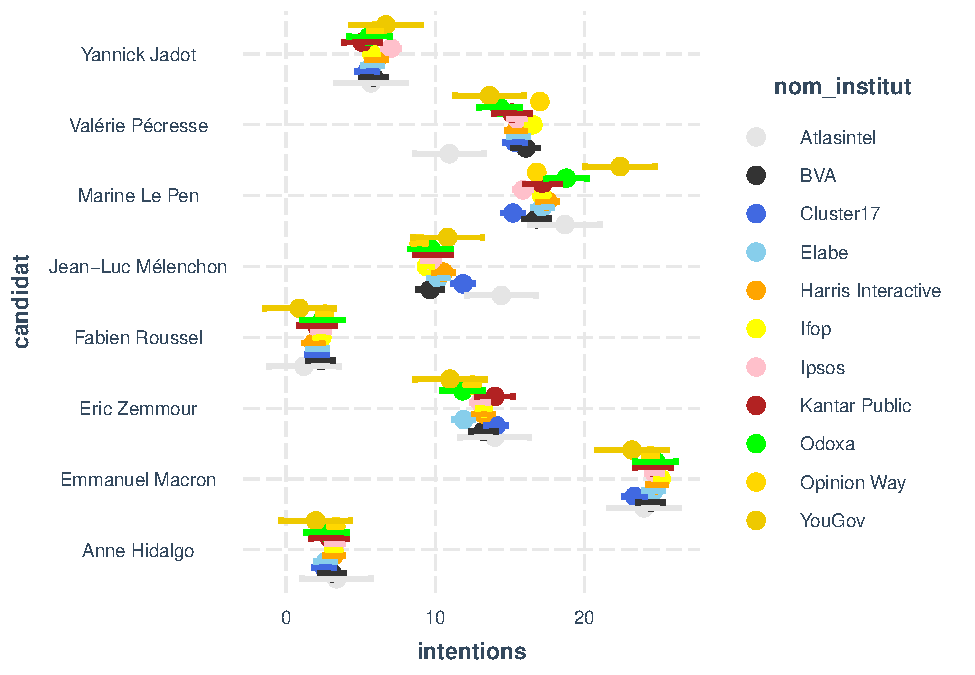
\includegraphics{bookdown-demo_files/figure-latex/biais-1.pdf}

\begin{Shaded}
\begin{Highlighting}[]
\KeywordTok{cat_plot}\NormalTok{(fit2, }\DataTypeTok{pred=}\NormalTok{ tps,}\DataTypeTok{modx=}\NormalTok{candidat, }\DataTypeTok{color.class=}\StringTok{"Spectral"}\NormalTok{, }\DataTypeTok{dodge.width=}\DecValTok{0}\NormalTok{)}\OperatorTok{+}
\StringTok{  }\KeywordTok{scale_color_manual}\NormalTok{(}\DataTypeTok{values =}\NormalTok{ SensiP2)}\OperatorTok{+}\KeywordTok{geom_line}\NormalTok{(}\KeywordTok{aes}\NormalTok{(}\DataTypeTok{color=}\NormalTok{candidat))}
\end{Highlighting}
\end{Shaded}

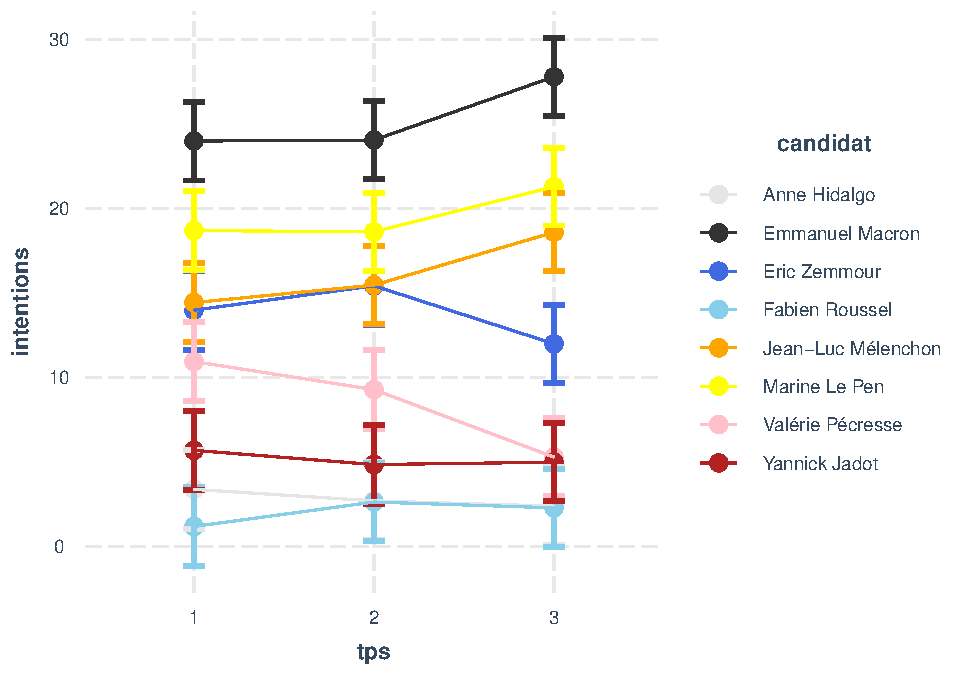
\includegraphics{bookdown-demo_files/figure-latex/biais-2.pdf}

\hypertarget{analyses-factorielles}{%
\chapter{Analyses factorielles}\label{analyses-factorielles}}

\hypertarget{origine-et-histoire}{%
\section{Origine et histoire}\label{origine-et-histoire}}

Par analyse factorielle, on entend finalement un ensemble de méthodes dont l'objectifs est d'extraire d'un ensemble multivariée de données, un petit nombre de dimensions, les facteurs, qui rendent compte l'essentiel des variations. Elles partagent aussi une même structure mathématique qui permet de décomposer et de réduire une matrice de données en un ensemble de matrice de dimensions réduite.

On peut en distinguer deux écoles, l'une alimentée par des questions de psychométrie a nourrit plusieurs decennies de recherche en traitant les tests psychométriques. L'autre française s'intéressent aux variables qualitatives, et a une perspective plus descriptive et représentationnelle.

\hypertarget{une-petite-histoire-de-la-psychomuxe9trie}{%
\subsection{Une petite histoire de la psychométrie}\label{une-petite-histoire-de-la-psychomuxe9trie}}

L'analyse factorielle trouve son origine, en psychologie, dans l'intuition que dans des épreuves multiples un facteur principal contrôle les variation des items (les performance à différents tests). Mais c'est avec Thurstone que l'idée prend toute son ampleur en permettant que plusieurs facteurs traduisent la structure de la matrice de corrélations entre les tests. Spearman, hotelling,.

Dans le monde de la gestion et en particulier de la GRH et du marketing, largement inspirés par la psychologie et la psychologie sociale, ces méthodes se sont propagées et ont formalisé un processus d'étude largement fondé sur ces techniques. Il est bien connu par de processus de Churchill qui a synthésisé une manière de construire et de développé des instruments de mesure par questionnaire. C'est l' article de historique de Churchill ( ref).

\hypertarget{luxe9cole-franuxe7aise-de-lanalyse-des-donnuxe9es-appliquuxe9e-aux-sciences-sociales}{%
\subsection{L'école française de l'analyse des données appliquée aux sciences sociales}\label{luxe9cole-franuxe7aise-de-lanalyse-des-donnuxe9es-appliquuxe9e-aux-sciences-sociales}}

Un personnage : Emile Benzekri

Boudieu en premier applicateurs

Une école Française : pagès, escoffier, morisseau, Husson a repris le flambleau en développant FactoMiner.

Une série de logiciels : Alceste, Statitcf

\hypertarget{le-moduxe8le-factoriel-des-tests-psychologiques}{%
\section{Le modèle factoriel des tests psychologiques}\label{le-moduxe8le-factoriel-des-tests-psychologiques}}

\hypertarget{un-peu-de-thuxe9orie}{%
\subsection{Un peu de théorie}\label{un-peu-de-thuxe9orie}}

La première historiquement est celle des psychologues et en particulier le modèle en terme de facteurs communs et spécifiques. Elle vise à partir de l'analyse d'une matrice de corrélation à identifier des éléments de structures sous-jascents.

La structure du modèle factoriel peut être présentée de manière simple. On supposera que chaque variables observées peut être décrites comme composées de facteurs généraux (\(F_{ik}\) ) et de facteurs spécifiques \$ \varepsilon\_\{i\}\$. Le modèle suppose ainsi que la valeur de l'individu i pour la variable j, dépend de k facteurs sous jascents, les facteurs communs, et d'un terme spécifique à l'item et à l'individus

\$\$
x\_\{ij\}= a\_\{1j\}F\_\{i1\} + a\_\{2j\}F\_\{i2\} + \cdots + a\_\{jk\}F\_\{ik\}+\varepsilon\_\{ij\}

\$\$

On peut représenter celà de manière plus graphique, en utilisant les conventions symboliques des modèles structurels qu'on examine dans le chapitre 9. On y verra d'ailleurs comment ce modèle peut être spécifié de manière confirmatoire.

On remarquera dans cette structure que les facteurs peuvent être corrélés.

\begin{figure}
\centering
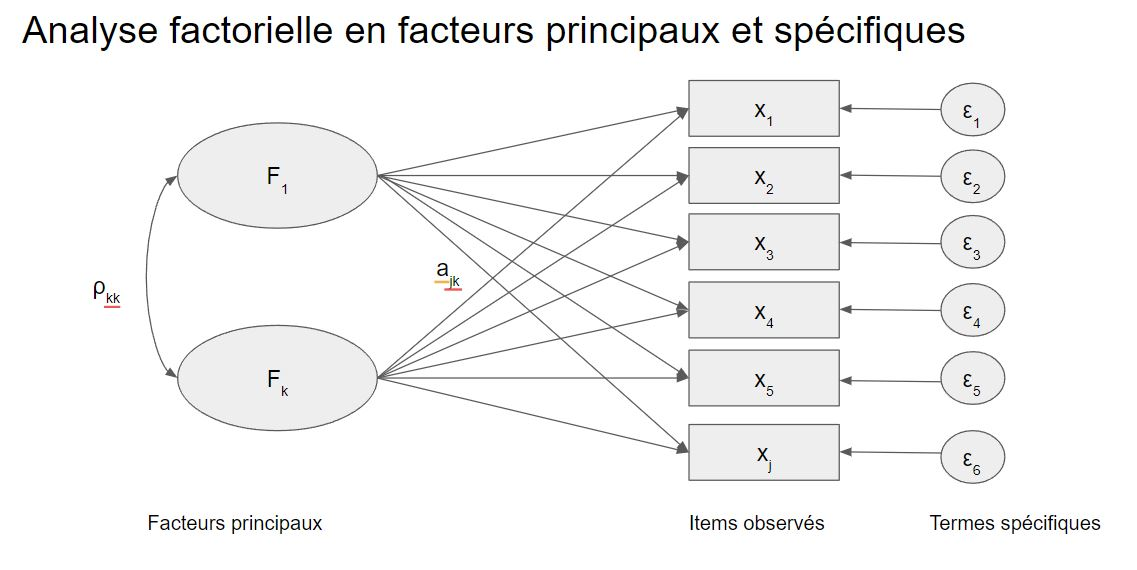
\includegraphics{./Images/FA01.jpg}
\caption{Modèle Factoriel exploratoire - EFA}
\end{figure}

\hypertarget{lestimation}{%
\subsection{L'estimation}\label{lestimation}}

Certains lecteurs seront surpris de cette présentation, ils sont sans doute plus habitués à factoriser en employant une méthode de l' ACP. Effectivement cette méthode sur laquelle on va revenir avec plus de détail dans la seconde section de ce chapitre, est une des techniques qui permettent d'approcher le modèle théorique que l'on vient de présenter. Elle n'est pas la seule.

L'estimation du modèle requierts deux décisions : l'une sur la méthode d'extraction des facteurs, et l'autres sur la méthode de rotation.

les méthodes d'extraction

\begin{itemize}
\tightlist
\item
  ACP
\item
  ML
\item
  analyse en facteur principaux et spécifiques
\end{itemize}

Les méthodes de rotation.

\begin{itemize}
\tightlist
\item
  Varimax
\item
  Promax
\item
  Oblimin
\item
  \ldots{}
\end{itemize}

\hypertarget{ressources}{%
\subsection{Ressources}\label{ressources}}

On utilise principalement le package \texttt{psych} développé par Revelle et dédié à la psychométrie. Il couvre le plus complétement le champs de l'analyse factorielle et de la psychométrie.

S'y ajoutent deux fonctions très utiles pour représenter le résultats des analyses sous une forme lisible et au standard des publications scientifiques. Elles utilisent les ressources de \texttt{flextable}.

\begin{Shaded}
\begin{Highlighting}[]
\CommentTok{#library(corrplot)}
\CommentTok{#library(psych)}
\CommentTok{#library(flextable)}


\CommentTok{# Une fonction utile pour créer }


\NormalTok{flex <-}\StringTok{ }\ControlFlowTok{function}\NormalTok{(data, }\DataTypeTok{title=}\OtherTok{NULL}\NormalTok{) \{}
  \CommentTok{# this grabs the data and converts it to a flextbale}
  \KeywordTok{flextable}\NormalTok{(data) }\OperatorTok
\StringTok{  }\CommentTok{# this makes the table fill the page width}
\StringTok{  }\KeywordTok{set_table_properties}\NormalTok{(}\DataTypeTok{layout =} \StringTok{"autofit"}\NormalTok{, }\DataTypeTok{width =} \DecValTok{1}\NormalTok{) }\OperatorTok
\StringTok{  }\CommentTok{# font size}
\StringTok{  }\KeywordTok{fontsize}\NormalTok{(}\DataTypeTok{size=}\DecValTok{10}\NormalTok{, }\DataTypeTok{part=}\StringTok{"all"}\NormalTok{) }\OperatorTok
\StringTok{    }\CommentTok{#this adds a ttitlecreates an automatic table number}
\StringTok{      }\KeywordTok{set_caption}\NormalTok{(title, }
                  \DataTypeTok{autonum =}\NormalTok{ officer}\OperatorTok{::}\KeywordTok{run_autonum}\NormalTok{(}\DataTypeTok{seq_id =} \StringTok{"tab"}\NormalTok{, }
                                                 \DataTypeTok{pre_label =} \StringTok{"Table "}\NormalTok{, }
                                                 \DataTypeTok{post_label =} \StringTok{"}\CharTok{\textbackslash{}n}\StringTok{"}\NormalTok{, }
                                                 \DataTypeTok{bkm =} \StringTok{"anytable"}\NormalTok{)) }\OperatorTok
\StringTok{  }\CommentTok{# font type}
\StringTok{  }\KeywordTok{font}\NormalTok{(}\DataTypeTok{fontname=}\StringTok{"Times New Roman"}\NormalTok{, }\DataTypeTok{part=}\StringTok{"all"}\NormalTok{)}
\NormalTok{\}}

\CommentTok{# et une seconde fonction pour le tableaux des loadings}


\NormalTok{fa_table <-}\StringTok{ }\ControlFlowTok{function}\NormalTok{(x, cut) \{}
  \CommentTok{#get sorted loadings}
\NormalTok{  loadings <-}\StringTok{ }\KeywordTok{fa.sort}\NormalTok{(x)}\OperatorTok{$}\NormalTok{loadings }\OperatorTok\StringTok{ }\KeywordTok{round}\NormalTok{(}\DecValTok{3}\NormalTok{)}
  \CommentTok{#supress loadings}
\NormalTok{  loadings[loadings }\OperatorTok{<}\StringTok{ }\NormalTok{cut] <-}\StringTok{ ""}
  \CommentTok{#get additional info}
\NormalTok{  add_info <-}\StringTok{ }\KeywordTok{cbind}\NormalTok{(x}\OperatorTok{$}\NormalTok{communality, }
\NormalTok{                    x}\OperatorTok{$}\NormalTok{uniquenesses,}
\NormalTok{                    x}\OperatorTok{$}\NormalTok{complexity) }\OperatorTok
\StringTok{    }\CommentTok{# make it a data frame}
\StringTok{    }\KeywordTok{as.data.frame}\NormalTok{() }\OperatorTok
\StringTok{    }\CommentTok{# column names}
\StringTok{    }\KeywordTok{rename}\NormalTok{(}\StringTok{"Communality"}\NormalTok{ =}\StringTok{ }\NormalTok{V1,}
           \StringTok{"Uniqueness"}\NormalTok{ =}\StringTok{ }\NormalTok{V2,}
           \StringTok{"Complexity"}\NormalTok{ =}\StringTok{ }\NormalTok{V3) }\OperatorTok
\StringTok{    }\CommentTok{#get the item names from the vector}
\StringTok{    }\KeywordTok{rownames_to_column}\NormalTok{(}\StringTok{"item"}\NormalTok{)}
  \CommentTok{#build table}
\NormalTok{  loadings }\OperatorTok
\StringTok{    }\KeywordTok{unclass}\NormalTok{() }\OperatorTok
\StringTok{    }\KeywordTok{as.data.frame}\NormalTok{() }\OperatorTok
\StringTok{    }\KeywordTok{rownames_to_column}\NormalTok{(}\StringTok{"item"}\NormalTok{) }\OperatorTok
\StringTok{    }\KeywordTok{left_join}\NormalTok{(add_info) }\OperatorTok
\StringTok{    }\KeywordTok{mutate}\NormalTok{(}\KeywordTok{across}\NormalTok{(}\KeywordTok{where}\NormalTok{(is.numeric), round, }\DecValTok{3}\NormalTok{))}
\NormalTok{\}}
\end{Highlighting}
\end{Shaded}

L'objectif des méthodes d'analyses factorielles est de réduire un ensemble de variables à un petit nombre de dimensions qui résument l'essentiel de l'information.

\hypertarget{cas-dapplication}{%
\subsection{Cas d'application}\label{cas-dapplication}}

Pour appliquer la méthode on va s'interesser à l'échelle des valeurs de kahle qui sont mesurée dan différents pays au cours des différentes vagues de l'enquête ESS?

Les variables mesurées sont un ensemble de 21 questions qui proposent des niveaux d'importances accordées à 21 questions, ou items, dont voici les formulation en anglais. Les répondants ont le choix sur une échelle de 0 à 10 qui va de ``pas du tout important'' à ``très important''. On se concentre sur les observations de la dernière vague.

Cette échelle a été développée par kahle.

En voici les itms dans leur formulation anglaise.

\begin{itemize}
\tightlist
\item
  IPCRTIV Important to think new ideas and being creative
\item
  IMPRICH Important to be rich, have money and expensive things
\item
  IPEQOPT Important that people are treated equally and have equal opportunities
\item
  IPSHABT Important to show abilities and be admired
\item
  IMPSAFE Important to live in secure and safe surroundings
\item
  IMPDIFF Important to try new and different things in life
\item
  IPFRULE Important to do what is told and follow rules
\item
  IPUDRST Important to understand different people
\item
  IPMODST Important to be humble and modest, not draw attention
\item
  IPGDTIM Important to have a good time
\item
  IMPFREE Important to make own decisions and be free
\item
  IPHLPPL Important to help people and care for others well-being
\item
  IPSUCES Important to be successful and that people recognise achievements
\item
  IPSTRGV Important that government is strong and ensures safety
\item
  IPADVNT Important to seek adventures and have an exciting life
\item
  IPBHPRP Important to behave properly
\item
  IPRSPOT Important to get respect from others
\item
  IPLYLFR Important to be loyal to friends and devote to people close
\item
  IMPENV Important to care for nature and environment
\item
  IMPTRAD Important to follow traditions and customs
\item
  IMPFUN Important to seek fun and things that give pleasure
\end{itemize}

\begin{Shaded}
\begin{Highlighting}[]
\CommentTok{# On renomme les variables pour une meilleure lecture et on selectionne le tableau de données utile à l'analyse.}

\NormalTok{df <-}\StringTok{ }\KeywordTok{read_csv}\NormalTok{(}\StringTok{"./Data/ESS1-9e01_1.csv"}\NormalTok{) }\OperatorTok
\StringTok{  }\KeywordTok{rename}\NormalTok{(}
    \DataTypeTok{V_creative=}\NormalTok{ipcrtiv,}
    \DataTypeTok{V_richness=}\NormalTok{ imprich,}
    \DataTypeTok{V_justice =}\NormalTok{ipeqopt, }
    \DataTypeTok{V_admiration=}\NormalTok{ipshabt, }
    \DataTypeTok{V_security=}\NormalTok{impsafe, }
    \DataTypeTok{V_novelty=}\NormalTok{impdiff, }
    \DataTypeTok{V_conformism=}\NormalTok{ipfrule, }
    \DataTypeTok{V_openmindedness=}\NormalTok{ipudrst, }
    \DataTypeTok{V_modesty=}\NormalTok{ipmodst, }
    \DataTypeTok{V_fun=}\NormalTok{ipgdtim, }
    \DataTypeTok{V_autonomy=}\NormalTok{impfree, }
    \DataTypeTok{V_Care=}\NormalTok{iphlppl, }
    \DataTypeTok{V_Success=}\NormalTok{ipsuces,}
    \DataTypeTok{V_Autority =}\NormalTok{ipstrgv, }
    \DataTypeTok{V_Adventures=}\NormalTok{ipadvnt,}
    \DataTypeTok{V_wellbehavior=}\NormalTok{ipbhprp,}
    \DataTypeTok{V_respect=}\NormalTok{iprspot,}
    \DataTypeTok{V_loyalty=}\NormalTok{iplylfr,}
    \DataTypeTok{V_environnement=}\NormalTok{impenv,}
    \DataTypeTok{V_tradition=}\NormalTok{imptrad, }
    \DataTypeTok{V_pleasure=}\NormalTok{impfun)}

\NormalTok{foo1<-df }\OperatorTok\StringTok{ }\KeywordTok{filter}\NormalTok{(essround}\OperatorTok{==}\DecValTok{9}\NormalTok{)}\OperatorTok
\StringTok{  }\NormalTok{dplyr}\OperatorTok{::}\KeywordTok{select}\NormalTok{(}\KeywordTok{matches}\NormalTok{(}\StringTok{"V_.*"}\NormalTok{), cntry) }\OperatorTok\StringTok{ }\CommentTok{#notons la selection fondée sur des regex}
\StringTok{  }\KeywordTok{drop_na}\NormalTok{()}
\end{Highlighting}
\end{Shaded}

\hypertarget{examen-de-la-matrice-de-corruxe9lation}{%
\section{Examen de la matrice de corrélation}\label{examen-de-la-matrice-de-corruxe9lation}}

Calculons la matrice de corrélation, et présentons là en organisant l'ordre des variables selon leur corrélation. A ce stade indiquons qu'il s'agit de mettre un ordre dans les variables, tel que des variables fortement corrélées soient adjascentes (on revient sur la méthode utilisée dans le chapitre suivant).

On s'aperçoit qu'une structure émerge. Quatre groupes de variables peuvent être discernées:
* la jouissance
* le succès social
* l'ouverture aux autres
* la sécurité

Dans le filigrane de la matrice de corrélation, on devine une structure factorielle.

\begin{Shaded}
\begin{Highlighting}[]
\NormalTok{foo<-}\StringTok{ }\NormalTok{foo1 }\OperatorTok\StringTok{ }
\StringTok{  }\NormalTok{dplyr}\OperatorTok{::}\KeywordTok{select}\NormalTok{(}\KeywordTok{matches}\NormalTok{(}\StringTok{"V_.*"}\NormalTok{))}

\NormalTok{M =}\StringTok{ }\KeywordTok{cor}\NormalTok{(foo)}

\KeywordTok{corrplot}\NormalTok{(M, }\DataTypeTok{method=}\StringTok{"circle"}\NormalTok{, }\DataTypeTok{order=}\StringTok{"hclust"}\NormalTok{,}\DataTypeTok{tl.cex =} \FloatTok{.7}\NormalTok{)}
\end{Highlighting}
\end{Shaded}

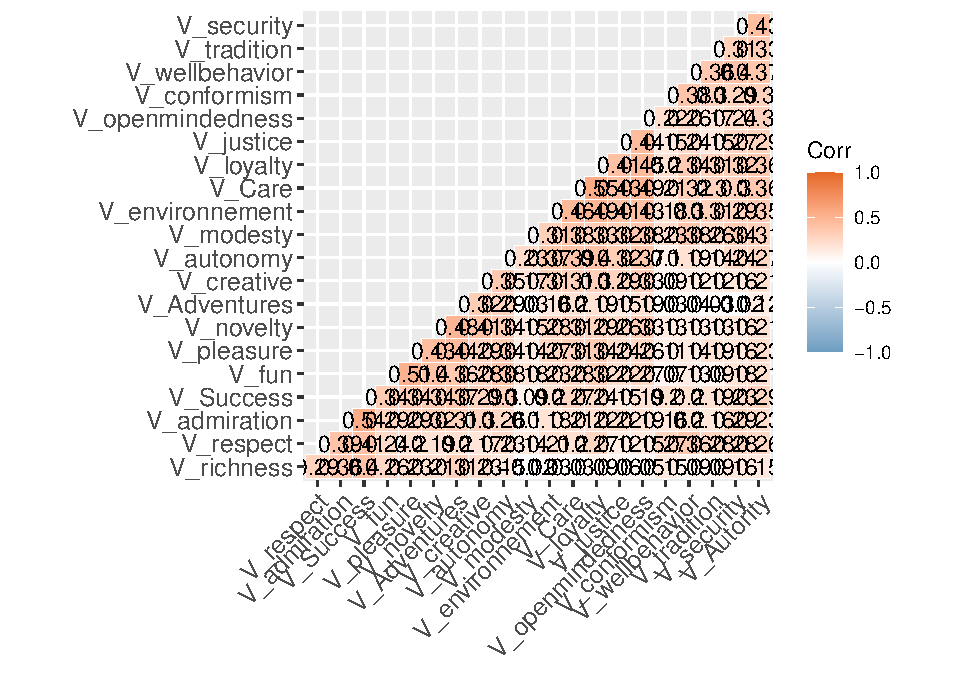
\includegraphics{bookdown-demo_files/figure-latex/0603b-1.pdf}

\hypertarget{moduxe8le-factoriel}{%
\section{Modèle factoriel}\label{moduxe8le-factoriel}}

Testons un modèle d'analyse factorielle à 4 dimensions. Nous l'augmentons d'un procédure de rotation oblimin pour un meilleur ajustement.

\begin{Shaded}
\begin{Highlighting}[]
\NormalTok{fa <-}\StringTok{ }\KeywordTok{fa}\NormalTok{(foo,}\DecValTok{4}\NormalTok{, }\DataTypeTok{rotate=}\StringTok{"oblimin"}\NormalTok{)  }\CommentTok{#principal axis }

\KeywordTok{fa_table}\NormalTok{(fa, }\FloatTok{.30}\NormalTok{)}\OperatorTok
\StringTok{  }\KeywordTok{flex}\NormalTok{(}\StringTok{"A Pretty Factor Analysis Table"}\NormalTok{)}
\end{Highlighting}
\end{Shaded}

\providecommand{\docline}[3]{\noalign{\global\setlength{\arrayrulewidth}{#1}}\arrayrulecolor[HTML]{#2}\cline{#3}}

\setlength{\tabcolsep}{2pt}

\renewcommand*{\arraystretch}{1.5}

\begin{longtable}[c]{cccccccc}

\caption{A Pretty Factor Analysis Table}\label{tab:anytable}\\

\hhline{>{\arrayrulecolor[HTML]{666666}\global\arrayrulewidth=2pt}->{\arrayrulecolor[HTML]{666666}\global\arrayrulewidth=2pt}->{\arrayrulecolor[HTML]{666666}\global\arrayrulewidth=2pt}->{\arrayrulecolor[HTML]{666666}\global\arrayrulewidth=2pt}->{\arrayrulecolor[HTML]{666666}\global\arrayrulewidth=2pt}->{\arrayrulecolor[HTML]{666666}\global\arrayrulewidth=2pt}->{\arrayrulecolor[HTML]{666666}\global\arrayrulewidth=2pt}->{\arrayrulecolor[HTML]{666666}\global\arrayrulewidth=2pt}-}

\multicolumn{1}{!{\color[HTML]{000000}\vrule width 0pt}>{}l}{\fontsize{10}{10}\selectfont{\textcolor[HTML]{000000}{\global\setmainfont{Times New Roman}{item}}}} & \multicolumn{1}{!{\color[HTML]{000000}\vrule width 0pt}>{}l}{\fontsize{10}{10}\selectfont{\textcolor[HTML]{000000}{\global\setmainfont{Times New Roman}{MR1}}}} & \multicolumn{1}{!{\color[HTML]{000000}\vrule width 0pt}>{}l}{\fontsize{10}{10}\selectfont{\textcolor[HTML]{000000}{\global\setmainfont{Times New Roman}{MR4}}}} & \multicolumn{1}{!{\color[HTML]{000000}\vrule width 0pt}>{}l}{\fontsize{10}{10}\selectfont{\textcolor[HTML]{000000}{\global\setmainfont{Times New Roman}{MR3}}}} & \multicolumn{1}{!{\color[HTML]{000000}\vrule width 0pt}>{}l}{\fontsize{10}{10}\selectfont{\textcolor[HTML]{000000}{\global\setmainfont{Times New Roman}{MR2}}}} & \multicolumn{1}{!{\color[HTML]{000000}\vrule width 0pt}>{}r}{\fontsize{10}{10}\selectfont{\textcolor[HTML]{000000}{\global\setmainfont{Times New Roman}{Communality}}}} & \multicolumn{1}{!{\color[HTML]{000000}\vrule width 0pt}>{}r}{\fontsize{10}{10}\selectfont{\textcolor[HTML]{000000}{\global\setmainfont{Times New Roman}{Uniqueness}}}} & \multicolumn{1}{!{\color[HTML]{000000}\vrule width 0pt}>{}r!{\color[HTML]{000000}\vrule width 0pt}}{\fontsize{10}{10}\selectfont{\textcolor[HTML]{000000}{\global\setmainfont{Times New Roman}{Complexity}}}} \\

\noalign{\global\setlength{\arrayrulewidth}{2pt}}\arrayrulecolor[HTML]{666666}\cline{1-8}

\endfirsthead

\hhline{>{\arrayrulecolor[HTML]{666666}\global\arrayrulewidth=2pt}->{\arrayrulecolor[HTML]{666666}\global\arrayrulewidth=2pt}->{\arrayrulecolor[HTML]{666666}\global\arrayrulewidth=2pt}->{\arrayrulecolor[HTML]{666666}\global\arrayrulewidth=2pt}->{\arrayrulecolor[HTML]{666666}\global\arrayrulewidth=2pt}->{\arrayrulecolor[HTML]{666666}\global\arrayrulewidth=2pt}->{\arrayrulecolor[HTML]{666666}\global\arrayrulewidth=2pt}->{\arrayrulecolor[HTML]{666666}\global\arrayrulewidth=2pt}-}

\multicolumn{1}{!{\color[HTML]{000000}\vrule width 0pt}>{}l}{\fontsize{10}{10}\selectfont{\textcolor[HTML]{000000}{\global\setmainfont{Times New Roman}{item}}}} & \multicolumn{1}{!{\color[HTML]{000000}\vrule width 0pt}>{}l}{\fontsize{10}{10}\selectfont{\textcolor[HTML]{000000}{\global\setmainfont{Times New Roman}{MR1}}}} & \multicolumn{1}{!{\color[HTML]{000000}\vrule width 0pt}>{}l}{\fontsize{10}{10}\selectfont{\textcolor[HTML]{000000}{\global\setmainfont{Times New Roman}{MR4}}}} & \multicolumn{1}{!{\color[HTML]{000000}\vrule width 0pt}>{}l}{\fontsize{10}{10}\selectfont{\textcolor[HTML]{000000}{\global\setmainfont{Times New Roman}{MR3}}}} & \multicolumn{1}{!{\color[HTML]{000000}\vrule width 0pt}>{}l}{\fontsize{10}{10}\selectfont{\textcolor[HTML]{000000}{\global\setmainfont{Times New Roman}{MR2}}}} & \multicolumn{1}{!{\color[HTML]{000000}\vrule width 0pt}>{}r}{\fontsize{10}{10}\selectfont{\textcolor[HTML]{000000}{\global\setmainfont{Times New Roman}{Communality}}}} & \multicolumn{1}{!{\color[HTML]{000000}\vrule width 0pt}>{}r}{\fontsize{10}{10}\selectfont{\textcolor[HTML]{000000}{\global\setmainfont{Times New Roman}{Uniqueness}}}} & \multicolumn{1}{!{\color[HTML]{000000}\vrule width 0pt}>{}r!{\color[HTML]{000000}\vrule width 0pt}}{\fontsize{10}{10}\selectfont{\textcolor[HTML]{000000}{\global\setmainfont{Times New Roman}{Complexity}}}} \\

\noalign{\global\setlength{\arrayrulewidth}{2pt}}\arrayrulecolor[HTML]{666666}\cline{1-8}\endhead



\multicolumn{1}{!{\color[HTML]{000000}\vrule width 0pt}>{}l}{\fontsize{10}{10}\selectfont{\textcolor[HTML]{000000}{\global\setmainfont{Times New Roman}{V\_openmindedness}}}} & \multicolumn{1}{!{\color[HTML]{000000}\vrule width 0pt}>{}l}{\fontsize{10}{10}\selectfont{\textcolor[HTML]{000000}{\global\setmainfont{Times New Roman}{0.692}}}} & \multicolumn{1}{!{\color[HTML]{000000}\vrule width 0pt}>{}l}{\fontsize{10}{10}\selectfont{\textcolor[HTML]{000000}{\global\setmainfont{Times New Roman}{}}}} & \multicolumn{1}{!{\color[HTML]{000000}\vrule width 0pt}>{}l}{\fontsize{10}{10}\selectfont{\textcolor[HTML]{000000}{\global\setmainfont{Times New Roman}{}}}} & \multicolumn{1}{!{\color[HTML]{000000}\vrule width 0pt}>{}l}{\fontsize{10}{10}\selectfont{\textcolor[HTML]{000000}{\global\setmainfont{Times New Roman}{}}}} & \multicolumn{1}{!{\color[HTML]{000000}\vrule width 0pt}>{}r}{\fontsize{10}{10}\selectfont{\textcolor[HTML]{000000}{\global\setmainfont{Times New Roman}{0.472}}}} & \multicolumn{1}{!{\color[HTML]{000000}\vrule width 0pt}>{}r}{\fontsize{10}{10}\selectfont{\textcolor[HTML]{000000}{\global\setmainfont{Times New Roman}{0.528}}}} & \multicolumn{1}{!{\color[HTML]{000000}\vrule width 0pt}>{}r!{\color[HTML]{000000}\vrule width 0pt}}{\fontsize{10}{10}\selectfont{\textcolor[HTML]{000000}{\global\setmainfont{Times New Roman}{1.002}}}} \\





\multicolumn{1}{!{\color[HTML]{000000}\vrule width 0pt}>{}l}{\fontsize{10}{10}\selectfont{\textcolor[HTML]{000000}{\global\setmainfont{Times New Roman}{V\_justice}}}} & \multicolumn{1}{!{\color[HTML]{000000}\vrule width 0pt}>{}l}{\fontsize{10}{10}\selectfont{\textcolor[HTML]{000000}{\global\setmainfont{Times New Roman}{0.665}}}} & \multicolumn{1}{!{\color[HTML]{000000}\vrule width 0pt}>{}l}{\fontsize{10}{10}\selectfont{\textcolor[HTML]{000000}{\global\setmainfont{Times New Roman}{}}}} & \multicolumn{1}{!{\color[HTML]{000000}\vrule width 0pt}>{}l}{\fontsize{10}{10}\selectfont{\textcolor[HTML]{000000}{\global\setmainfont{Times New Roman}{}}}} & \multicolumn{1}{!{\color[HTML]{000000}\vrule width 0pt}>{}l}{\fontsize{10}{10}\selectfont{\textcolor[HTML]{000000}{\global\setmainfont{Times New Roman}{}}}} & \multicolumn{1}{!{\color[HTML]{000000}\vrule width 0pt}>{}r}{\fontsize{10}{10}\selectfont{\textcolor[HTML]{000000}{\global\setmainfont{Times New Roman}{0.399}}}} & \multicolumn{1}{!{\color[HTML]{000000}\vrule width 0pt}>{}r}{\fontsize{10}{10}\selectfont{\textcolor[HTML]{000000}{\global\setmainfont{Times New Roman}{0.601}}}} & \multicolumn{1}{!{\color[HTML]{000000}\vrule width 0pt}>{}r!{\color[HTML]{000000}\vrule width 0pt}}{\fontsize{10}{10}\selectfont{\textcolor[HTML]{000000}{\global\setmainfont{Times New Roman}{1.044}}}} \\





\multicolumn{1}{!{\color[HTML]{000000}\vrule width 0pt}>{}l}{\fontsize{10}{10}\selectfont{\textcolor[HTML]{000000}{\global\setmainfont{Times New Roman}{V\_Care}}}} & \multicolumn{1}{!{\color[HTML]{000000}\vrule width 0pt}>{}l}{\fontsize{10}{10}\selectfont{\textcolor[HTML]{000000}{\global\setmainfont{Times New Roman}{0.621}}}} & \multicolumn{1}{!{\color[HTML]{000000}\vrule width 0pt}>{}l}{\fontsize{10}{10}\selectfont{\textcolor[HTML]{000000}{\global\setmainfont{Times New Roman}{}}}} & \multicolumn{1}{!{\color[HTML]{000000}\vrule width 0pt}>{}l}{\fontsize{10}{10}\selectfont{\textcolor[HTML]{000000}{\global\setmainfont{Times New Roman}{}}}} & \multicolumn{1}{!{\color[HTML]{000000}\vrule width 0pt}>{}l}{\fontsize{10}{10}\selectfont{\textcolor[HTML]{000000}{\global\setmainfont{Times New Roman}{}}}} & \multicolumn{1}{!{\color[HTML]{000000}\vrule width 0pt}>{}r}{\fontsize{10}{10}\selectfont{\textcolor[HTML]{000000}{\global\setmainfont{Times New Roman}{0.516}}}} & \multicolumn{1}{!{\color[HTML]{000000}\vrule width 0pt}>{}r}{\fontsize{10}{10}\selectfont{\textcolor[HTML]{000000}{\global\setmainfont{Times New Roman}{0.484}}}} & \multicolumn{1}{!{\color[HTML]{000000}\vrule width 0pt}>{}r!{\color[HTML]{000000}\vrule width 0pt}}{\fontsize{10}{10}\selectfont{\textcolor[HTML]{000000}{\global\setmainfont{Times New Roman}{1.145}}}} \\





\multicolumn{1}{!{\color[HTML]{000000}\vrule width 0pt}>{}l}{\fontsize{10}{10}\selectfont{\textcolor[HTML]{000000}{\global\setmainfont{Times New Roman}{V\_environnement}}}} & \multicolumn{1}{!{\color[HTML]{000000}\vrule width 0pt}>{}l}{\fontsize{10}{10}\selectfont{\textcolor[HTML]{000000}{\global\setmainfont{Times New Roman}{0.561}}}} & \multicolumn{1}{!{\color[HTML]{000000}\vrule width 0pt}>{}l}{\fontsize{10}{10}\selectfont{\textcolor[HTML]{000000}{\global\setmainfont{Times New Roman}{}}}} & \multicolumn{1}{!{\color[HTML]{000000}\vrule width 0pt}>{}l}{\fontsize{10}{10}\selectfont{\textcolor[HTML]{000000}{\global\setmainfont{Times New Roman}{}}}} & \multicolumn{1}{!{\color[HTML]{000000}\vrule width 0pt}>{}l}{\fontsize{10}{10}\selectfont{\textcolor[HTML]{000000}{\global\setmainfont{Times New Roman}{}}}} & \multicolumn{1}{!{\color[HTML]{000000}\vrule width 0pt}>{}r}{\fontsize{10}{10}\selectfont{\textcolor[HTML]{000000}{\global\setmainfont{Times New Roman}{0.427}}}} & \multicolumn{1}{!{\color[HTML]{000000}\vrule width 0pt}>{}r}{\fontsize{10}{10}\selectfont{\textcolor[HTML]{000000}{\global\setmainfont{Times New Roman}{0.573}}}} & \multicolumn{1}{!{\color[HTML]{000000}\vrule width 0pt}>{}r!{\color[HTML]{000000}\vrule width 0pt}}{\fontsize{10}{10}\selectfont{\textcolor[HTML]{000000}{\global\setmainfont{Times New Roman}{1.171}}}} \\





\multicolumn{1}{!{\color[HTML]{000000}\vrule width 0pt}>{}l}{\fontsize{10}{10}\selectfont{\textcolor[HTML]{000000}{\global\setmainfont{Times New Roman}{V\_loyalty}}}} & \multicolumn{1}{!{\color[HTML]{000000}\vrule width 0pt}>{}l}{\fontsize{10}{10}\selectfont{\textcolor[HTML]{000000}{\global\setmainfont{Times New Roman}{0.518}}}} & \multicolumn{1}{!{\color[HTML]{000000}\vrule width 0pt}>{}l}{\fontsize{10}{10}\selectfont{\textcolor[HTML]{000000}{\global\setmainfont{Times New Roman}{}}}} & \multicolumn{1}{!{\color[HTML]{000000}\vrule width 0pt}>{}l}{\fontsize{10}{10}\selectfont{\textcolor[HTML]{000000}{\global\setmainfont{Times New Roman}{}}}} & \multicolumn{1}{!{\color[HTML]{000000}\vrule width 0pt}>{}l}{\fontsize{10}{10}\selectfont{\textcolor[HTML]{000000}{\global\setmainfont{Times New Roman}{}}}} & \multicolumn{1}{!{\color[HTML]{000000}\vrule width 0pt}>{}r}{\fontsize{10}{10}\selectfont{\textcolor[HTML]{000000}{\global\setmainfont{Times New Roman}{0.493}}}} & \multicolumn{1}{!{\color[HTML]{000000}\vrule width 0pt}>{}r}{\fontsize{10}{10}\selectfont{\textcolor[HTML]{000000}{\global\setmainfont{Times New Roman}{0.507}}}} & \multicolumn{1}{!{\color[HTML]{000000}\vrule width 0pt}>{}r!{\color[HTML]{000000}\vrule width 0pt}}{\fontsize{10}{10}\selectfont{\textcolor[HTML]{000000}{\global\setmainfont{Times New Roman}{1.570}}}} \\





\multicolumn{1}{!{\color[HTML]{000000}\vrule width 0pt}>{}l}{\fontsize{10}{10}\selectfont{\textcolor[HTML]{000000}{\global\setmainfont{Times New Roman}{V\_autonomy}}}} & \multicolumn{1}{!{\color[HTML]{000000}\vrule width 0pt}>{}l}{\fontsize{10}{10}\selectfont{\textcolor[HTML]{000000}{\global\setmainfont{Times New Roman}{0.438}}}} & \multicolumn{1}{!{\color[HTML]{000000}\vrule width 0pt}>{}l}{\fontsize{10}{10}\selectfont{\textcolor[HTML]{000000}{\global\setmainfont{Times New Roman}{}}}} & \multicolumn{1}{!{\color[HTML]{000000}\vrule width 0pt}>{}l}{\fontsize{10}{10}\selectfont{\textcolor[HTML]{000000}{\global\setmainfont{Times New Roman}{}}}} & \multicolumn{1}{!{\color[HTML]{000000}\vrule width 0pt}>{}l}{\fontsize{10}{10}\selectfont{\textcolor[HTML]{000000}{\global\setmainfont{Times New Roman}{}}}} & \multicolumn{1}{!{\color[HTML]{000000}\vrule width 0pt}>{}r}{\fontsize{10}{10}\selectfont{\textcolor[HTML]{000000}{\global\setmainfont{Times New Roman}{0.364}}}} & \multicolumn{1}{!{\color[HTML]{000000}\vrule width 0pt}>{}r}{\fontsize{10}{10}\selectfont{\textcolor[HTML]{000000}{\global\setmainfont{Times New Roman}{0.636}}}} & \multicolumn{1}{!{\color[HTML]{000000}\vrule width 0pt}>{}r!{\color[HTML]{000000}\vrule width 0pt}}{\fontsize{10}{10}\selectfont{\textcolor[HTML]{000000}{\global\setmainfont{Times New Roman}{1.603}}}} \\





\multicolumn{1}{!{\color[HTML]{000000}\vrule width 0pt}>{}l}{\fontsize{10}{10}\selectfont{\textcolor[HTML]{000000}{\global\setmainfont{Times New Roman}{V\_creative}}}} & \multicolumn{1}{!{\color[HTML]{000000}\vrule width 0pt}>{}l}{\fontsize{10}{10}\selectfont{\textcolor[HTML]{000000}{\global\setmainfont{Times New Roman}{0.429}}}} & \multicolumn{1}{!{\color[HTML]{000000}\vrule width 0pt}>{}l}{\fontsize{10}{10}\selectfont{\textcolor[HTML]{000000}{\global\setmainfont{Times New Roman}{}}}} & \multicolumn{1}{!{\color[HTML]{000000}\vrule width 0pt}>{}l}{\fontsize{10}{10}\selectfont{\textcolor[HTML]{000000}{\global\setmainfont{Times New Roman}{}}}} & \multicolumn{1}{!{\color[HTML]{000000}\vrule width 0pt}>{}l}{\fontsize{10}{10}\selectfont{\textcolor[HTML]{000000}{\global\setmainfont{Times New Roman}{}}}} & \multicolumn{1}{!{\color[HTML]{000000}\vrule width 0pt}>{}r}{\fontsize{10}{10}\selectfont{\textcolor[HTML]{000000}{\global\setmainfont{Times New Roman}{0.341}}}} & \multicolumn{1}{!{\color[HTML]{000000}\vrule width 0pt}>{}r}{\fontsize{10}{10}\selectfont{\textcolor[HTML]{000000}{\global\setmainfont{Times New Roman}{0.659}}}} & \multicolumn{1}{!{\color[HTML]{000000}\vrule width 0pt}>{}r!{\color[HTML]{000000}\vrule width 0pt}}{\fontsize{10}{10}\selectfont{\textcolor[HTML]{000000}{\global\setmainfont{Times New Roman}{2.225}}}} \\





\multicolumn{1}{!{\color[HTML]{000000}\vrule width 0pt}>{}l}{\fontsize{10}{10}\selectfont{\textcolor[HTML]{000000}{\global\setmainfont{Times New Roman}{V\_modesty}}}} & \multicolumn{1}{!{\color[HTML]{000000}\vrule width 0pt}>{}l}{\fontsize{10}{10}\selectfont{\textcolor[HTML]{000000}{\global\setmainfont{Times New Roman}{0.421}}}} & \multicolumn{1}{!{\color[HTML]{000000}\vrule width 0pt}>{}l}{\fontsize{10}{10}\selectfont{\textcolor[HTML]{000000}{\global\setmainfont{Times New Roman}{}}}} & \multicolumn{1}{!{\color[HTML]{000000}\vrule width 0pt}>{}l}{\fontsize{10}{10}\selectfont{\textcolor[HTML]{000000}{\global\setmainfont{Times New Roman}{0.301}}}} & \multicolumn{1}{!{\color[HTML]{000000}\vrule width 0pt}>{}l}{\fontsize{10}{10}\selectfont{\textcolor[HTML]{000000}{\global\setmainfont{Times New Roman}{}}}} & \multicolumn{1}{!{\color[HTML]{000000}\vrule width 0pt}>{}r}{\fontsize{10}{10}\selectfont{\textcolor[HTML]{000000}{\global\setmainfont{Times New Roman}{0.339}}}} & \multicolumn{1}{!{\color[HTML]{000000}\vrule width 0pt}>{}r}{\fontsize{10}{10}\selectfont{\textcolor[HTML]{000000}{\global\setmainfont{Times New Roman}{0.661}}}} & \multicolumn{1}{!{\color[HTML]{000000}\vrule width 0pt}>{}r!{\color[HTML]{000000}\vrule width 0pt}}{\fontsize{10}{10}\selectfont{\textcolor[HTML]{000000}{\global\setmainfont{Times New Roman}{1.967}}}} \\





\multicolumn{1}{!{\color[HTML]{000000}\vrule width 0pt}>{}l}{\fontsize{10}{10}\selectfont{\textcolor[HTML]{000000}{\global\setmainfont{Times New Roman}{V\_admiration}}}} & \multicolumn{1}{!{\color[HTML]{000000}\vrule width 0pt}>{}l}{\fontsize{10}{10}\selectfont{\textcolor[HTML]{000000}{\global\setmainfont{Times New Roman}{}}}} & \multicolumn{1}{!{\color[HTML]{000000}\vrule width 0pt}>{}l}{\fontsize{10}{10}\selectfont{\textcolor[HTML]{000000}{\global\setmainfont{Times New Roman}{0.697}}}} & \multicolumn{1}{!{\color[HTML]{000000}\vrule width 0pt}>{}l}{\fontsize{10}{10}\selectfont{\textcolor[HTML]{000000}{\global\setmainfont{Times New Roman}{}}}} & \multicolumn{1}{!{\color[HTML]{000000}\vrule width 0pt}>{}l}{\fontsize{10}{10}\selectfont{\textcolor[HTML]{000000}{\global\setmainfont{Times New Roman}{}}}} & \multicolumn{1}{!{\color[HTML]{000000}\vrule width 0pt}>{}r}{\fontsize{10}{10}\selectfont{\textcolor[HTML]{000000}{\global\setmainfont{Times New Roman}{0.505}}}} & \multicolumn{1}{!{\color[HTML]{000000}\vrule width 0pt}>{}r}{\fontsize{10}{10}\selectfont{\textcolor[HTML]{000000}{\global\setmainfont{Times New Roman}{0.495}}}} & \multicolumn{1}{!{\color[HTML]{000000}\vrule width 0pt}>{}r!{\color[HTML]{000000}\vrule width 0pt}}{\fontsize{10}{10}\selectfont{\textcolor[HTML]{000000}{\global\setmainfont{Times New Roman}{1.049}}}} \\





\multicolumn{1}{!{\color[HTML]{000000}\vrule width 0pt}>{}l}{\fontsize{10}{10}\selectfont{\textcolor[HTML]{000000}{\global\setmainfont{Times New Roman}{V\_Success}}}} & \multicolumn{1}{!{\color[HTML]{000000}\vrule width 0pt}>{}l}{\fontsize{10}{10}\selectfont{\textcolor[HTML]{000000}{\global\setmainfont{Times New Roman}{}}}} & \multicolumn{1}{!{\color[HTML]{000000}\vrule width 0pt}>{}l}{\fontsize{10}{10}\selectfont{\textcolor[HTML]{000000}{\global\setmainfont{Times New Roman}{0.644}}}} & \multicolumn{1}{!{\color[HTML]{000000}\vrule width 0pt}>{}l}{\fontsize{10}{10}\selectfont{\textcolor[HTML]{000000}{\global\setmainfont{Times New Roman}{}}}} & \multicolumn{1}{!{\color[HTML]{000000}\vrule width 0pt}>{}l}{\fontsize{10}{10}\selectfont{\textcolor[HTML]{000000}{\global\setmainfont{Times New Roman}{}}}} & \multicolumn{1}{!{\color[HTML]{000000}\vrule width 0pt}>{}r}{\fontsize{10}{10}\selectfont{\textcolor[HTML]{000000}{\global\setmainfont{Times New Roman}{0.539}}}} & \multicolumn{1}{!{\color[HTML]{000000}\vrule width 0pt}>{}r}{\fontsize{10}{10}\selectfont{\textcolor[HTML]{000000}{\global\setmainfont{Times New Roman}{0.461}}}} & \multicolumn{1}{!{\color[HTML]{000000}\vrule width 0pt}>{}r!{\color[HTML]{000000}\vrule width 0pt}}{\fontsize{10}{10}\selectfont{\textcolor[HTML]{000000}{\global\setmainfont{Times New Roman}{1.094}}}} \\





\multicolumn{1}{!{\color[HTML]{000000}\vrule width 0pt}>{}l}{\fontsize{10}{10}\selectfont{\textcolor[HTML]{000000}{\global\setmainfont{Times New Roman}{V\_richness}}}} & \multicolumn{1}{!{\color[HTML]{000000}\vrule width 0pt}>{}l}{\fontsize{10}{10}\selectfont{\textcolor[HTML]{000000}{\global\setmainfont{Times New Roman}{}}}} & \multicolumn{1}{!{\color[HTML]{000000}\vrule width 0pt}>{}l}{\fontsize{10}{10}\selectfont{\textcolor[HTML]{000000}{\global\setmainfont{Times New Roman}{0.526}}}} & \multicolumn{1}{!{\color[HTML]{000000}\vrule width 0pt}>{}l}{\fontsize{10}{10}\selectfont{\textcolor[HTML]{000000}{\global\setmainfont{Times New Roman}{}}}} & \multicolumn{1}{!{\color[HTML]{000000}\vrule width 0pt}>{}l}{\fontsize{10}{10}\selectfont{\textcolor[HTML]{000000}{\global\setmainfont{Times New Roman}{}}}} & \multicolumn{1}{!{\color[HTML]{000000}\vrule width 0pt}>{}r}{\fontsize{10}{10}\selectfont{\textcolor[HTML]{000000}{\global\setmainfont{Times New Roman}{0.336}}}} & \multicolumn{1}{!{\color[HTML]{000000}\vrule width 0pt}>{}r}{\fontsize{10}{10}\selectfont{\textcolor[HTML]{000000}{\global\setmainfont{Times New Roman}{0.664}}}} & \multicolumn{1}{!{\color[HTML]{000000}\vrule width 0pt}>{}r!{\color[HTML]{000000}\vrule width 0pt}}{\fontsize{10}{10}\selectfont{\textcolor[HTML]{000000}{\global\setmainfont{Times New Roman}{1.402}}}} \\





\multicolumn{1}{!{\color[HTML]{000000}\vrule width 0pt}>{}l}{\fontsize{10}{10}\selectfont{\textcolor[HTML]{000000}{\global\setmainfont{Times New Roman}{V\_respect}}}} & \multicolumn{1}{!{\color[HTML]{000000}\vrule width 0pt}>{}l}{\fontsize{10}{10}\selectfont{\textcolor[HTML]{000000}{\global\setmainfont{Times New Roman}{}}}} & \multicolumn{1}{!{\color[HTML]{000000}\vrule width 0pt}>{}l}{\fontsize{10}{10}\selectfont{\textcolor[HTML]{000000}{\global\setmainfont{Times New Roman}{0.419}}}} & \multicolumn{1}{!{\color[HTML]{000000}\vrule width 0pt}>{}l}{\fontsize{10}{10}\selectfont{\textcolor[HTML]{000000}{\global\setmainfont{Times New Roman}{0.379}}}} & \multicolumn{1}{!{\color[HTML]{000000}\vrule width 0pt}>{}l}{\fontsize{10}{10}\selectfont{\textcolor[HTML]{000000}{\global\setmainfont{Times New Roman}{}}}} & \multicolumn{1}{!{\color[HTML]{000000}\vrule width 0pt}>{}r}{\fontsize{10}{10}\selectfont{\textcolor[HTML]{000000}{\global\setmainfont{Times New Roman}{0.383}}}} & \multicolumn{1}{!{\color[HTML]{000000}\vrule width 0pt}>{}r}{\fontsize{10}{10}\selectfont{\textcolor[HTML]{000000}{\global\setmainfont{Times New Roman}{0.617}}}} & \multicolumn{1}{!{\color[HTML]{000000}\vrule width 0pt}>{}r!{\color[HTML]{000000}\vrule width 0pt}}{\fontsize{10}{10}\selectfont{\textcolor[HTML]{000000}{\global\setmainfont{Times New Roman}{2.157}}}} \\





\multicolumn{1}{!{\color[HTML]{000000}\vrule width 0pt}>{}l}{\fontsize{10}{10}\selectfont{\textcolor[HTML]{000000}{\global\setmainfont{Times New Roman}{V\_wellbehavior}}}} & \multicolumn{1}{!{\color[HTML]{000000}\vrule width 0pt}>{}l}{\fontsize{10}{10}\selectfont{\textcolor[HTML]{000000}{\global\setmainfont{Times New Roman}{}}}} & \multicolumn{1}{!{\color[HTML]{000000}\vrule width 0pt}>{}l}{\fontsize{10}{10}\selectfont{\textcolor[HTML]{000000}{\global\setmainfont{Times New Roman}{}}}} & \multicolumn{1}{!{\color[HTML]{000000}\vrule width 0pt}>{}l}{\fontsize{10}{10}\selectfont{\textcolor[HTML]{000000}{\global\setmainfont{Times New Roman}{0.604}}}} & \multicolumn{1}{!{\color[HTML]{000000}\vrule width 0pt}>{}l}{\fontsize{10}{10}\selectfont{\textcolor[HTML]{000000}{\global\setmainfont{Times New Roman}{}}}} & \multicolumn{1}{!{\color[HTML]{000000}\vrule width 0pt}>{}r}{\fontsize{10}{10}\selectfont{\textcolor[HTML]{000000}{\global\setmainfont{Times New Roman}{0.461}}}} & \multicolumn{1}{!{\color[HTML]{000000}\vrule width 0pt}>{}r}{\fontsize{10}{10}\selectfont{\textcolor[HTML]{000000}{\global\setmainfont{Times New Roman}{0.539}}}} & \multicolumn{1}{!{\color[HTML]{000000}\vrule width 0pt}>{}r!{\color[HTML]{000000}\vrule width 0pt}}{\fontsize{10}{10}\selectfont{\textcolor[HTML]{000000}{\global\setmainfont{Times New Roman}{1.094}}}} \\





\multicolumn{1}{!{\color[HTML]{000000}\vrule width 0pt}>{}l}{\fontsize{10}{10}\selectfont{\textcolor[HTML]{000000}{\global\setmainfont{Times New Roman}{V\_tradition}}}} & \multicolumn{1}{!{\color[HTML]{000000}\vrule width 0pt}>{}l}{\fontsize{10}{10}\selectfont{\textcolor[HTML]{000000}{\global\setmainfont{Times New Roman}{}}}} & \multicolumn{1}{!{\color[HTML]{000000}\vrule width 0pt}>{}l}{\fontsize{10}{10}\selectfont{\textcolor[HTML]{000000}{\global\setmainfont{Times New Roman}{}}}} & \multicolumn{1}{!{\color[HTML]{000000}\vrule width 0pt}>{}l}{\fontsize{10}{10}\selectfont{\textcolor[HTML]{000000}{\global\setmainfont{Times New Roman}{0.531}}}} & \multicolumn{1}{!{\color[HTML]{000000}\vrule width 0pt}>{}l}{\fontsize{10}{10}\selectfont{\textcolor[HTML]{000000}{\global\setmainfont{Times New Roman}{}}}} & \multicolumn{1}{!{\color[HTML]{000000}\vrule width 0pt}>{}r}{\fontsize{10}{10}\selectfont{\textcolor[HTML]{000000}{\global\setmainfont{Times New Roman}{0.323}}}} & \multicolumn{1}{!{\color[HTML]{000000}\vrule width 0pt}>{}r}{\fontsize{10}{10}\selectfont{\textcolor[HTML]{000000}{\global\setmainfont{Times New Roman}{0.677}}}} & \multicolumn{1}{!{\color[HTML]{000000}\vrule width 0pt}>{}r!{\color[HTML]{000000}\vrule width 0pt}}{\fontsize{10}{10}\selectfont{\textcolor[HTML]{000000}{\global\setmainfont{Times New Roman}{1.111}}}} \\





\multicolumn{1}{!{\color[HTML]{000000}\vrule width 0pt}>{}l}{\fontsize{10}{10}\selectfont{\textcolor[HTML]{000000}{\global\setmainfont{Times New Roman}{V\_conformism}}}} & \multicolumn{1}{!{\color[HTML]{000000}\vrule width 0pt}>{}l}{\fontsize{10}{10}\selectfont{\textcolor[HTML]{000000}{\global\setmainfont{Times New Roman}{}}}} & \multicolumn{1}{!{\color[HTML]{000000}\vrule width 0pt}>{}l}{\fontsize{10}{10}\selectfont{\textcolor[HTML]{000000}{\global\setmainfont{Times New Roman}{}}}} & \multicolumn{1}{!{\color[HTML]{000000}\vrule width 0pt}>{}l}{\fontsize{10}{10}\selectfont{\textcolor[HTML]{000000}{\global\setmainfont{Times New Roman}{0.464}}}} & \multicolumn{1}{!{\color[HTML]{000000}\vrule width 0pt}>{}l}{\fontsize{10}{10}\selectfont{\textcolor[HTML]{000000}{\global\setmainfont{Times New Roman}{}}}} & \multicolumn{1}{!{\color[HTML]{000000}\vrule width 0pt}>{}r}{\fontsize{10}{10}\selectfont{\textcolor[HTML]{000000}{\global\setmainfont{Times New Roman}{0.265}}}} & \multicolumn{1}{!{\color[HTML]{000000}\vrule width 0pt}>{}r}{\fontsize{10}{10}\selectfont{\textcolor[HTML]{000000}{\global\setmainfont{Times New Roman}{0.735}}}} & \multicolumn{1}{!{\color[HTML]{000000}\vrule width 0pt}>{}r!{\color[HTML]{000000}\vrule width 0pt}}{\fontsize{10}{10}\selectfont{\textcolor[HTML]{000000}{\global\setmainfont{Times New Roman}{1.166}}}} \\





\multicolumn{1}{!{\color[HTML]{000000}\vrule width 0pt}>{}l}{\fontsize{10}{10}\selectfont{\textcolor[HTML]{000000}{\global\setmainfont{Times New Roman}{V\_security}}}} & \multicolumn{1}{!{\color[HTML]{000000}\vrule width 0pt}>{}l}{\fontsize{10}{10}\selectfont{\textcolor[HTML]{000000}{\global\setmainfont{Times New Roman}{}}}} & \multicolumn{1}{!{\color[HTML]{000000}\vrule width 0pt}>{}l}{\fontsize{10}{10}\selectfont{\textcolor[HTML]{000000}{\global\setmainfont{Times New Roman}{}}}} & \multicolumn{1}{!{\color[HTML]{000000}\vrule width 0pt}>{}l}{\fontsize{10}{10}\selectfont{\textcolor[HTML]{000000}{\global\setmainfont{Times New Roman}{0.445}}}} & \multicolumn{1}{!{\color[HTML]{000000}\vrule width 0pt}>{}l}{\fontsize{10}{10}\selectfont{\textcolor[HTML]{000000}{\global\setmainfont{Times New Roman}{}}}} & \multicolumn{1}{!{\color[HTML]{000000}\vrule width 0pt}>{}r}{\fontsize{10}{10}\selectfont{\textcolor[HTML]{000000}{\global\setmainfont{Times New Roman}{0.386}}}} & \multicolumn{1}{!{\color[HTML]{000000}\vrule width 0pt}>{}r}{\fontsize{10}{10}\selectfont{\textcolor[HTML]{000000}{\global\setmainfont{Times New Roman}{0.614}}}} & \multicolumn{1}{!{\color[HTML]{000000}\vrule width 0pt}>{}r!{\color[HTML]{000000}\vrule width 0pt}}{\fontsize{10}{10}\selectfont{\textcolor[HTML]{000000}{\global\setmainfont{Times New Roman}{2.047}}}} \\





\multicolumn{1}{!{\color[HTML]{000000}\vrule width 0pt}>{}l}{\fontsize{10}{10}\selectfont{\textcolor[HTML]{000000}{\global\setmainfont{Times New Roman}{V\_Autority}}}} & \multicolumn{1}{!{\color[HTML]{000000}\vrule width 0pt}>{}l}{\fontsize{10}{10}\selectfont{\textcolor[HTML]{000000}{\global\setmainfont{Times New Roman}{}}}} & \multicolumn{1}{!{\color[HTML]{000000}\vrule width 0pt}>{}l}{\fontsize{10}{10}\selectfont{\textcolor[HTML]{000000}{\global\setmainfont{Times New Roman}{}}}} & \multicolumn{1}{!{\color[HTML]{000000}\vrule width 0pt}>{}l}{\fontsize{10}{10}\selectfont{\textcolor[HTML]{000000}{\global\setmainfont{Times New Roman}{0.395}}}} & \multicolumn{1}{!{\color[HTML]{000000}\vrule width 0pt}>{}l}{\fontsize{10}{10}\selectfont{\textcolor[HTML]{000000}{\global\setmainfont{Times New Roman}{}}}} & \multicolumn{1}{!{\color[HTML]{000000}\vrule width 0pt}>{}r}{\fontsize{10}{10}\selectfont{\textcolor[HTML]{000000}{\global\setmainfont{Times New Roman}{0.369}}}} & \multicolumn{1}{!{\color[HTML]{000000}\vrule width 0pt}>{}r}{\fontsize{10}{10}\selectfont{\textcolor[HTML]{000000}{\global\setmainfont{Times New Roman}{0.631}}}} & \multicolumn{1}{!{\color[HTML]{000000}\vrule width 0pt}>{}r!{\color[HTML]{000000}\vrule width 0pt}}{\fontsize{10}{10}\selectfont{\textcolor[HTML]{000000}{\global\setmainfont{Times New Roman}{1.921}}}} \\





\multicolumn{1}{!{\color[HTML]{000000}\vrule width 0pt}>{}l}{\fontsize{10}{10}\selectfont{\textcolor[HTML]{000000}{\global\setmainfont{Times New Roman}{V\_pleasure}}}} & \multicolumn{1}{!{\color[HTML]{000000}\vrule width 0pt}>{}l}{\fontsize{10}{10}\selectfont{\textcolor[HTML]{000000}{\global\setmainfont{Times New Roman}{}}}} & \multicolumn{1}{!{\color[HTML]{000000}\vrule width 0pt}>{}l}{\fontsize{10}{10}\selectfont{\textcolor[HTML]{000000}{\global\setmainfont{Times New Roman}{}}}} & \multicolumn{1}{!{\color[HTML]{000000}\vrule width 0pt}>{}l}{\fontsize{10}{10}\selectfont{\textcolor[HTML]{000000}{\global\setmainfont{Times New Roman}{}}}} & \multicolumn{1}{!{\color[HTML]{000000}\vrule width 0pt}>{}l}{\fontsize{10}{10}\selectfont{\textcolor[HTML]{000000}{\global\setmainfont{Times New Roman}{0.758}}}} & \multicolumn{1}{!{\color[HTML]{000000}\vrule width 0pt}>{}r}{\fontsize{10}{10}\selectfont{\textcolor[HTML]{000000}{\global\setmainfont{Times New Roman}{0.561}}}} & \multicolumn{1}{!{\color[HTML]{000000}\vrule width 0pt}>{}r}{\fontsize{10}{10}\selectfont{\textcolor[HTML]{000000}{\global\setmainfont{Times New Roman}{0.439}}}} & \multicolumn{1}{!{\color[HTML]{000000}\vrule width 0pt}>{}r!{\color[HTML]{000000}\vrule width 0pt}}{\fontsize{10}{10}\selectfont{\textcolor[HTML]{000000}{\global\setmainfont{Times New Roman}{1.035}}}} \\





\multicolumn{1}{!{\color[HTML]{000000}\vrule width 0pt}>{}l}{\fontsize{10}{10}\selectfont{\textcolor[HTML]{000000}{\global\setmainfont{Times New Roman}{V\_fun}}}} & \multicolumn{1}{!{\color[HTML]{000000}\vrule width 0pt}>{}l}{\fontsize{10}{10}\selectfont{\textcolor[HTML]{000000}{\global\setmainfont{Times New Roman}{}}}} & \multicolumn{1}{!{\color[HTML]{000000}\vrule width 0pt}>{}l}{\fontsize{10}{10}\selectfont{\textcolor[HTML]{000000}{\global\setmainfont{Times New Roman}{}}}} & \multicolumn{1}{!{\color[HTML]{000000}\vrule width 0pt}>{}l}{\fontsize{10}{10}\selectfont{\textcolor[HTML]{000000}{\global\setmainfont{Times New Roman}{}}}} & \multicolumn{1}{!{\color[HTML]{000000}\vrule width 0pt}>{}l}{\fontsize{10}{10}\selectfont{\textcolor[HTML]{000000}{\global\setmainfont{Times New Roman}{0.531}}}} & \multicolumn{1}{!{\color[HTML]{000000}\vrule width 0pt}>{}r}{\fontsize{10}{10}\selectfont{\textcolor[HTML]{000000}{\global\setmainfont{Times New Roman}{0.413}}}} & \multicolumn{1}{!{\color[HTML]{000000}\vrule width 0pt}>{}r}{\fontsize{10}{10}\selectfont{\textcolor[HTML]{000000}{\global\setmainfont{Times New Roman}{0.587}}}} & \multicolumn{1}{!{\color[HTML]{000000}\vrule width 0pt}>{}r!{\color[HTML]{000000}\vrule width 0pt}}{\fontsize{10}{10}\selectfont{\textcolor[HTML]{000000}{\global\setmainfont{Times New Roman}{1.145}}}} \\





\multicolumn{1}{!{\color[HTML]{000000}\vrule width 0pt}>{}l}{\fontsize{10}{10}\selectfont{\textcolor[HTML]{000000}{\global\setmainfont{Times New Roman}{V\_Adventures}}}} & \multicolumn{1}{!{\color[HTML]{000000}\vrule width 0pt}>{}l}{\fontsize{10}{10}\selectfont{\textcolor[HTML]{000000}{\global\setmainfont{Times New Roman}{}}}} & \multicolumn{1}{!{\color[HTML]{000000}\vrule width 0pt}>{}l}{\fontsize{10}{10}\selectfont{\textcolor[HTML]{000000}{\global\setmainfont{Times New Roman}{}}}} & \multicolumn{1}{!{\color[HTML]{000000}\vrule width 0pt}>{}l}{\fontsize{10}{10}\selectfont{\textcolor[HTML]{000000}{\global\setmainfont{Times New Roman}{}}}} & \multicolumn{1}{!{\color[HTML]{000000}\vrule width 0pt}>{}l}{\fontsize{10}{10}\selectfont{\textcolor[HTML]{000000}{\global\setmainfont{Times New Roman}{0.506}}}} & \multicolumn{1}{!{\color[HTML]{000000}\vrule width 0pt}>{}r}{\fontsize{10}{10}\selectfont{\textcolor[HTML]{000000}{\global\setmainfont{Times New Roman}{0.465}}}} & \multicolumn{1}{!{\color[HTML]{000000}\vrule width 0pt}>{}r}{\fontsize{10}{10}\selectfont{\textcolor[HTML]{000000}{\global\setmainfont{Times New Roman}{0.535}}}} & \multicolumn{1}{!{\color[HTML]{000000}\vrule width 0pt}>{}r!{\color[HTML]{000000}\vrule width 0pt}}{\fontsize{10}{10}\selectfont{\textcolor[HTML]{000000}{\global\setmainfont{Times New Roman}{1.829}}}} \\





\multicolumn{1}{!{\color[HTML]{000000}\vrule width 0pt}>{}l}{\fontsize{10}{10}\selectfont{\textcolor[HTML]{000000}{\global\setmainfont{Times New Roman}{V\_novelty}}}} & \multicolumn{1}{!{\color[HTML]{000000}\vrule width 0pt}>{}l}{\fontsize{10}{10}\selectfont{\textcolor[HTML]{000000}{\global\setmainfont{Times New Roman}{}}}} & \multicolumn{1}{!{\color[HTML]{000000}\vrule width 0pt}>{}l}{\fontsize{10}{10}\selectfont{\textcolor[HTML]{000000}{\global\setmainfont{Times New Roman}{}}}} & \multicolumn{1}{!{\color[HTML]{000000}\vrule width 0pt}>{}l}{\fontsize{10}{10}\selectfont{\textcolor[HTML]{000000}{\global\setmainfont{Times New Roman}{}}}} & \multicolumn{1}{!{\color[HTML]{000000}\vrule width 0pt}>{}l}{\fontsize{10}{10}\selectfont{\textcolor[HTML]{000000}{\global\setmainfont{Times New Roman}{0.392}}}} & \multicolumn{1}{!{\color[HTML]{000000}\vrule width 0pt}>{}r}{\fontsize{10}{10}\selectfont{\textcolor[HTML]{000000}{\global\setmainfont{Times New Roman}{0.431}}}} & \multicolumn{1}{!{\color[HTML]{000000}\vrule width 0pt}>{}r}{\fontsize{10}{10}\selectfont{\textcolor[HTML]{000000}{\global\setmainfont{Times New Roman}{0.569}}}} & \multicolumn{1}{!{\color[HTML]{000000}\vrule width 0pt}>{}r!{\color[HTML]{000000}\vrule width 0pt}}{\fontsize{10}{10}\selectfont{\textcolor[HTML]{000000}{\global\setmainfont{Times New Roman}{2.553}}}} \\

\noalign{\global\setlength{\arrayrulewidth}{2pt}}\arrayrulecolor[HTML]{666666}\cline{1-8}



\end{longtable}

\begin{Shaded}
\begin{Highlighting}[]
\NormalTok{fa[[}\StringTok{"Vaccounted"}\NormalTok{]] }\OperatorTok
\StringTok{  }\KeywordTok{as.data.frame}\NormalTok{() }\OperatorTok
\StringTok{  }\CommentTok{#select(1:5) %>% Use this if you have many factors and only want to show a certain number}
\StringTok{  }\KeywordTok{rownames_to_column}\NormalTok{(}\StringTok{"Property"}\NormalTok{) }\OperatorTok
\StringTok{    }\KeywordTok{mutate}\NormalTok{(}\KeywordTok{across}\NormalTok{(}\KeywordTok{where}\NormalTok{(is.numeric), round, }\DecValTok{3}\NormalTok{)) }\OperatorTok
\StringTok{    }\KeywordTok{flex}\NormalTok{(}\StringTok{"Eigenvalues and Variance Explained for Rotated Factor Solution"}\NormalTok{)}
\end{Highlighting}
\end{Shaded}

\providecommand{\docline}[3]{\noalign{\global\setlength{\arrayrulewidth}{#1}}\arrayrulecolor[HTML]{#2}\cline{#3}}

\setlength{\tabcolsep}{2pt}

\renewcommand*{\arraystretch}{1.5}

\begin{longtable}[c]{ccccc}

\caption{Eigenvalues and Variance Explained for Rotated Factor Solution}\label{tab:anytable}\\

\hhline{>{\arrayrulecolor[HTML]{666666}\global\arrayrulewidth=2pt}->{\arrayrulecolor[HTML]{666666}\global\arrayrulewidth=2pt}->{\arrayrulecolor[HTML]{666666}\global\arrayrulewidth=2pt}->{\arrayrulecolor[HTML]{666666}\global\arrayrulewidth=2pt}->{\arrayrulecolor[HTML]{666666}\global\arrayrulewidth=2pt}-}

\multicolumn{1}{!{\color[HTML]{000000}\vrule width 0pt}>{}l}{\fontsize{10}{10}\selectfont{\textcolor[HTML]{000000}{\global\setmainfont{Times New Roman}{Property}}}} & \multicolumn{1}{!{\color[HTML]{000000}\vrule width 0pt}>{}r}{\fontsize{10}{10}\selectfont{\textcolor[HTML]{000000}{\global\setmainfont{Times New Roman}{MR1}}}} & \multicolumn{1}{!{\color[HTML]{000000}\vrule width 0pt}>{}r}{\fontsize{10}{10}\selectfont{\textcolor[HTML]{000000}{\global\setmainfont{Times New Roman}{MR4}}}} & \multicolumn{1}{!{\color[HTML]{000000}\vrule width 0pt}>{}r}{\fontsize{10}{10}\selectfont{\textcolor[HTML]{000000}{\global\setmainfont{Times New Roman}{MR3}}}} & \multicolumn{1}{!{\color[HTML]{000000}\vrule width 0pt}>{}r!{\color[HTML]{000000}\vrule width 0pt}}{\fontsize{10}{10}\selectfont{\textcolor[HTML]{000000}{\global\setmainfont{Times New Roman}{MR2}}}} \\

\noalign{\global\setlength{\arrayrulewidth}{2pt}}\arrayrulecolor[HTML]{666666}\cline{1-5}

\endfirsthead

\hhline{>{\arrayrulecolor[HTML]{666666}\global\arrayrulewidth=2pt}->{\arrayrulecolor[HTML]{666666}\global\arrayrulewidth=2pt}->{\arrayrulecolor[HTML]{666666}\global\arrayrulewidth=2pt}->{\arrayrulecolor[HTML]{666666}\global\arrayrulewidth=2pt}->{\arrayrulecolor[HTML]{666666}\global\arrayrulewidth=2pt}-}

\multicolumn{1}{!{\color[HTML]{000000}\vrule width 0pt}>{}l}{\fontsize{10}{10}\selectfont{\textcolor[HTML]{000000}{\global\setmainfont{Times New Roman}{Property}}}} & \multicolumn{1}{!{\color[HTML]{000000}\vrule width 0pt}>{}r}{\fontsize{10}{10}\selectfont{\textcolor[HTML]{000000}{\global\setmainfont{Times New Roman}{MR1}}}} & \multicolumn{1}{!{\color[HTML]{000000}\vrule width 0pt}>{}r}{\fontsize{10}{10}\selectfont{\textcolor[HTML]{000000}{\global\setmainfont{Times New Roman}{MR4}}}} & \multicolumn{1}{!{\color[HTML]{000000}\vrule width 0pt}>{}r}{\fontsize{10}{10}\selectfont{\textcolor[HTML]{000000}{\global\setmainfont{Times New Roman}{MR3}}}} & \multicolumn{1}{!{\color[HTML]{000000}\vrule width 0pt}>{}r!{\color[HTML]{000000}\vrule width 0pt}}{\fontsize{10}{10}\selectfont{\textcolor[HTML]{000000}{\global\setmainfont{Times New Roman}{MR2}}}} \\

\noalign{\global\setlength{\arrayrulewidth}{2pt}}\arrayrulecolor[HTML]{666666}\cline{1-5}\endhead



\multicolumn{1}{!{\color[HTML]{000000}\vrule width 0pt}>{}l}{\fontsize{10}{10}\selectfont{\textcolor[HTML]{000000}{\global\setmainfont{Times New Roman}{SS\ loadings}}}} & \multicolumn{1}{!{\color[HTML]{000000}\vrule width 0pt}>{}r}{\fontsize{10}{10}\selectfont{\textcolor[HTML]{000000}{\global\setmainfont{Times New Roman}{3.122}}}} & \multicolumn{1}{!{\color[HTML]{000000}\vrule width 0pt}>{}r}{\fontsize{10}{10}\selectfont{\textcolor[HTML]{000000}{\global\setmainfont{Times New Roman}{1.958}}}} & \multicolumn{1}{!{\color[HTML]{000000}\vrule width 0pt}>{}r}{\fontsize{10}{10}\selectfont{\textcolor[HTML]{000000}{\global\setmainfont{Times New Roman}{1.897}}}} & \multicolumn{1}{!{\color[HTML]{000000}\vrule width 0pt}>{}r!{\color[HTML]{000000}\vrule width 0pt}}{\fontsize{10}{10}\selectfont{\textcolor[HTML]{000000}{\global\setmainfont{Times New Roman}{1.813}}}} \\





\multicolumn{1}{!{\color[HTML]{000000}\vrule width 0pt}>{}l}{\fontsize{10}{10}\selectfont{\textcolor[HTML]{000000}{\global\setmainfont{Times New Roman}{Proportion\ Var}}}} & \multicolumn{1}{!{\color[HTML]{000000}\vrule width 0pt}>{}r}{\fontsize{10}{10}\selectfont{\textcolor[HTML]{000000}{\global\setmainfont{Times New Roman}{0.149}}}} & \multicolumn{1}{!{\color[HTML]{000000}\vrule width 0pt}>{}r}{\fontsize{10}{10}\selectfont{\textcolor[HTML]{000000}{\global\setmainfont{Times New Roman}{0.093}}}} & \multicolumn{1}{!{\color[HTML]{000000}\vrule width 0pt}>{}r}{\fontsize{10}{10}\selectfont{\textcolor[HTML]{000000}{\global\setmainfont{Times New Roman}{0.090}}}} & \multicolumn{1}{!{\color[HTML]{000000}\vrule width 0pt}>{}r!{\color[HTML]{000000}\vrule width 0pt}}{\fontsize{10}{10}\selectfont{\textcolor[HTML]{000000}{\global\setmainfont{Times New Roman}{0.086}}}} \\





\multicolumn{1}{!{\color[HTML]{000000}\vrule width 0pt}>{}l}{\fontsize{10}{10}\selectfont{\textcolor[HTML]{000000}{\global\setmainfont{Times New Roman}{Cumulative\ Var}}}} & \multicolumn{1}{!{\color[HTML]{000000}\vrule width 0pt}>{}r}{\fontsize{10}{10}\selectfont{\textcolor[HTML]{000000}{\global\setmainfont{Times New Roman}{0.149}}}} & \multicolumn{1}{!{\color[HTML]{000000}\vrule width 0pt}>{}r}{\fontsize{10}{10}\selectfont{\textcolor[HTML]{000000}{\global\setmainfont{Times New Roman}{0.242}}}} & \multicolumn{1}{!{\color[HTML]{000000}\vrule width 0pt}>{}r}{\fontsize{10}{10}\selectfont{\textcolor[HTML]{000000}{\global\setmainfont{Times New Roman}{0.332}}}} & \multicolumn{1}{!{\color[HTML]{000000}\vrule width 0pt}>{}r!{\color[HTML]{000000}\vrule width 0pt}}{\fontsize{10}{10}\selectfont{\textcolor[HTML]{000000}{\global\setmainfont{Times New Roman}{0.419}}}} \\





\multicolumn{1}{!{\color[HTML]{000000}\vrule width 0pt}>{}l}{\fontsize{10}{10}\selectfont{\textcolor[HTML]{000000}{\global\setmainfont{Times New Roman}{Proportion\ Explained}}}} & \multicolumn{1}{!{\color[HTML]{000000}\vrule width 0pt}>{}r}{\fontsize{10}{10}\selectfont{\textcolor[HTML]{000000}{\global\setmainfont{Times New Roman}{0.355}}}} & \multicolumn{1}{!{\color[HTML]{000000}\vrule width 0pt}>{}r}{\fontsize{10}{10}\selectfont{\textcolor[HTML]{000000}{\global\setmainfont{Times New Roman}{0.223}}}} & \multicolumn{1}{!{\color[HTML]{000000}\vrule width 0pt}>{}r}{\fontsize{10}{10}\selectfont{\textcolor[HTML]{000000}{\global\setmainfont{Times New Roman}{0.216}}}} & \multicolumn{1}{!{\color[HTML]{000000}\vrule width 0pt}>{}r!{\color[HTML]{000000}\vrule width 0pt}}{\fontsize{10}{10}\selectfont{\textcolor[HTML]{000000}{\global\setmainfont{Times New Roman}{0.206}}}} \\





\multicolumn{1}{!{\color[HTML]{000000}\vrule width 0pt}>{}l}{\fontsize{10}{10}\selectfont{\textcolor[HTML]{000000}{\global\setmainfont{Times New Roman}{Cumulative\ Proportion}}}} & \multicolumn{1}{!{\color[HTML]{000000}\vrule width 0pt}>{}r}{\fontsize{10}{10}\selectfont{\textcolor[HTML]{000000}{\global\setmainfont{Times New Roman}{0.355}}}} & \multicolumn{1}{!{\color[HTML]{000000}\vrule width 0pt}>{}r}{\fontsize{10}{10}\selectfont{\textcolor[HTML]{000000}{\global\setmainfont{Times New Roman}{0.578}}}} & \multicolumn{1}{!{\color[HTML]{000000}\vrule width 0pt}>{}r}{\fontsize{10}{10}\selectfont{\textcolor[HTML]{000000}{\global\setmainfont{Times New Roman}{0.794}}}} & \multicolumn{1}{!{\color[HTML]{000000}\vrule width 0pt}>{}r!{\color[HTML]{000000}\vrule width 0pt}}{\fontsize{10}{10}\selectfont{\textcolor[HTML]{000000}{\global\setmainfont{Times New Roman}{1.000}}}} \\

\noalign{\global\setlength{\arrayrulewidth}{2pt}}\arrayrulecolor[HTML]{666666}\cline{1-5}



\end{longtable}

Le set de données que nous avons traité est composé de 15 échantillons venant d'autant de pays. Puisque nous avons réduits les 22 mesures initiales à 4 grands facteurs, il est temps d'analyser les différences entre les pays.

On va d'abord récupérer les scores de chaque observation sur les quatre dimensions obtenues qu'on ajoute à notre fichier de travail pour récupérer la variable pays.

\begin{Shaded}
\begin{Highlighting}[]
\CommentTok{#récupérer les scores}

\NormalTok{scores<-fa}\OperatorTok{$}\NormalTok{scores}
\NormalTok{scores<-}\KeywordTok{as.data.frame}\NormalTok{(}\KeywordTok{unclass}\NormalTok{(scores))}

\CommentTok{#matcher pour récupérer la variable pays et renommer pour plus de lisibilité}

\NormalTok{df_typo<-}\KeywordTok{cbind}\NormalTok{(foo1, scores) }\OperatorTok\StringTok{ }
\StringTok{  }\KeywordTok{rename}\NormalTok{(}\DataTypeTok{F_Altruisme =}\NormalTok{ MR1, }
        \DataTypeTok{F_Conservatisme=}\NormalTok{MR2,}
        \DataTypeTok{F_Performance=}\NormalTok{MR4,}
        \DataTypeTok{F_Hedonisme=}\NormalTok{MR3)}

\CommentTok{# On calcule les scores moyens par pays et les erreurs d'échantillonage}
\NormalTok{df_g <-}\StringTok{ }\NormalTok{df_typo }\OperatorTok\StringTok{ }
\StringTok{  }\NormalTok{dplyr}\OperatorTok{::}\KeywordTok{select}\NormalTok{(}\KeywordTok{matches}\NormalTok{(}\StringTok{"F_.*"}\NormalTok{), cntry)}\OperatorTok
\StringTok{  }\KeywordTok{gather}\NormalTok{(variable, value,}\OperatorTok{-}\NormalTok{cntry)}\OperatorTok
\StringTok{  }\KeywordTok{mutate}\NormalTok{(}\DataTypeTok{n=}\DecValTok{1}\NormalTok{)}\OperatorTok
\StringTok{  }\KeywordTok{group_by}\NormalTok{(variable,cntry)}\OperatorTok\StringTok{ }
\StringTok{  }\KeywordTok{summarize}\NormalTok{(}\DataTypeTok{mean=}\KeywordTok{mean}\NormalTok{(value),}
            \DataTypeTok{n=}\KeywordTok{sum}\NormalTok{(n),}
            \DataTypeTok{se=}\KeywordTok{sd}\NormalTok{(value)}\OperatorTok{/}\KeywordTok{sqrt}\NormalTok{(n))}

\CommentTok{#on représente les résultats}

\KeywordTok{ggplot}\NormalTok{(df_g,}\KeywordTok{aes}\NormalTok{(}\DataTypeTok{x=}\NormalTok{cntry, }\DataTypeTok{y=}\NormalTok{mean))}\OperatorTok{+}
\StringTok{  }\KeywordTok{geom_bar}\NormalTok{(}\DataTypeTok{stat=}\StringTok{"identity"}\NormalTok{,}\KeywordTok{aes}\NormalTok{(}\DataTypeTok{fill=}\NormalTok{variable), }\DataTypeTok{size=}\FloatTok{1.5}\NormalTok{)}\OperatorTok{+}\StringTok{ }\KeywordTok{coord_flip}\NormalTok{()}\OperatorTok{+}
\StringTok{  }\KeywordTok{geom_errorbar}\NormalTok{(}\KeywordTok{aes}\NormalTok{(}\DataTypeTok{ymin=}\NormalTok{mean}\OperatorTok{-}\NormalTok{se, }\DataTypeTok{ymax=}\NormalTok{mean}\OperatorTok{+}\NormalTok{se), }\DataTypeTok{width=}\NormalTok{.}\DecValTok{2}\NormalTok{, }\DataTypeTok{position=}\KeywordTok{position_dodge}\NormalTok{(.}\DecValTok{9}\NormalTok{)) }\OperatorTok{+}
\StringTok{  }\KeywordTok{scale_color_brewer}\NormalTok{(}\DataTypeTok{palette =} \StringTok{"Set1"}\NormalTok{)}\OperatorTok{+}
\StringTok{  }\KeywordTok{facet_wrap}\NormalTok{(}\KeywordTok{vars}\NormalTok{(variable),}\DataTypeTok{ncol=}\DecValTok{2}\NormalTok{)}
\end{Highlighting}
\end{Shaded}

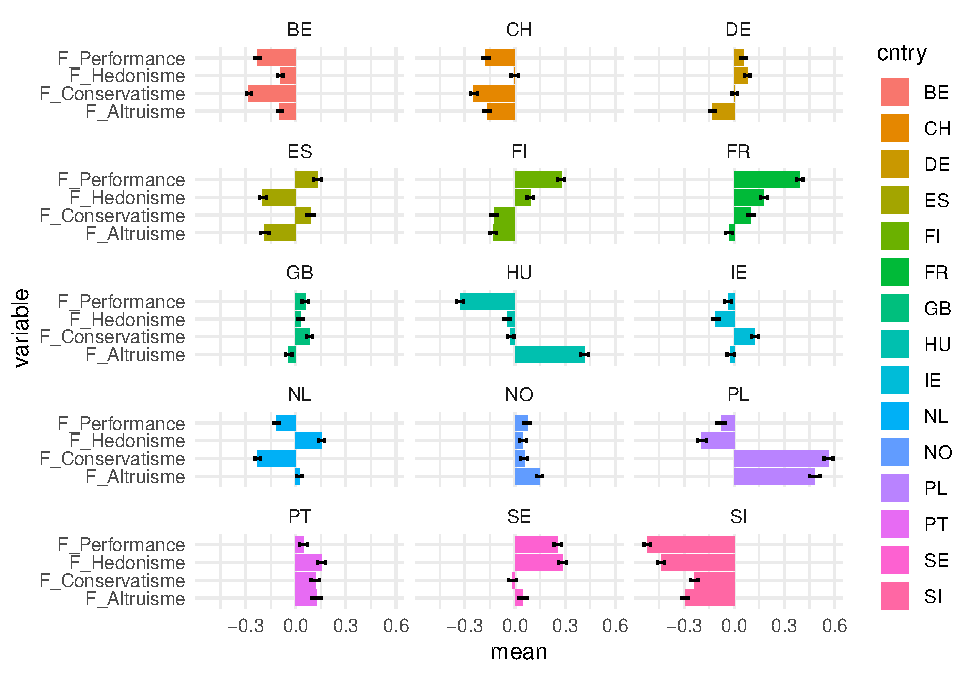
\includegraphics{bookdown-demo_files/figure-latex/0605-1.pdf}

\hypertarget{lanalyse-en-composante-principale}{%
\section{L'analyse en composante principale}\label{lanalyse-en-composante-principale}}

L'ACP, dont l'optique est différente dans le sens où l'on cherche moins à rendre compte d'une structure sous-jascente à la matrice de corrélation , qu'à réduire l'information dans un espace limité.

\hypertarget{le-probluxe8me-thuxe9orique}{%
\subsection{le problème théorique}\label{le-probluxe8me-thuxe9orique}}

De manière intuitive l'ACP est la technique qui permet de représenter un poisson, une structure, sous son jour le plus intelligible, c'est à dire celui qui magnifie ses variations.

Examinons un poisson sous différentes projections. La première image rend mieux compte de la forme du poisson que la seconde, elle ne diffère que par la projection. De l'une à l'autre il n'y a qu'y rotation à 90°C vers la droite. C'est la même image, le même phénomène mais représenté selon deux perspectives, deux bases en terme de mathématiques. On comprend que pour représenter un objet au mieux dans un faible nombre de dimensions, il faut trouver la base vectorielle qui maximise les variations de taille.

résoudre ce problème est ce que fait l'ACP

\begin{figure}
\centering
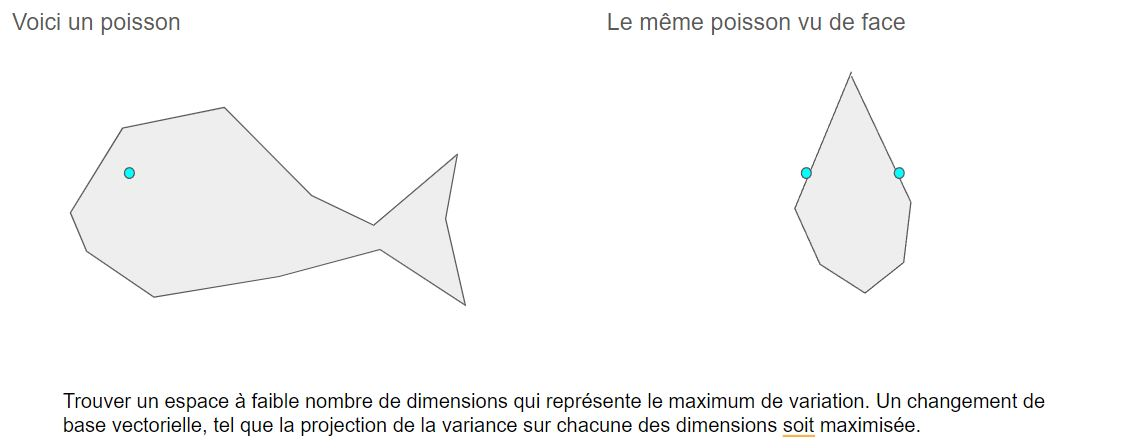
\includegraphics{./Images/ACp_poisson.jpg}
\caption{Modèle Factoriel exploratoire - EFA}
\end{figure}

\hypertarget{une-repruxe9sentation-symbolique}{%
\subsection{Une représentation symbolique}\label{une-repruxe9sentation-symbolique}}

L'idée va donc être de décomposer une matrice de variance-covariance (ou de corrélation) en respectant une contraintes : faire en sorte que le maximum de variance soit capturée par la première dimension, puis par les suivantes successivement. La solution à ce problème se trouve dans la résolution d'un problème matriciel. Il faut procéder à un changement de base, autrement dit à un changement de référentiel.

La matrice de variance-covariance, ou de corrélation, si on a, au préalable, centré et standardisé les valeurs des variables, est obtenue simplement en multipliant la matrice de données (individus x variable) par sa transposée.

\[
\Sigma = XX^t
\]
Comme \(\Sigma\) est symétrique, elle est diagonalisable et peut-être représentée par une matrice de score W et une matrice diagonale D.

\[
\Sigma_{e} =WDW^T
\]
où D est la matrice diagonale des valeurs propres et W la matrice des composantes comprenant les j variables ( en ligne) et les k dimensions (en colonne). L'équivalence suppose que le nombre de composantes est égal au nombre de variables initiales, Cependant l'usage conduit à ne retenir qu'un petit nombre de dimensions de telles sorte à ce que la différence entre \(\Sigma\) et \(\Sigma_{e}\) soit relativement petite. La matrice de score comprend autant de lignes que d'individus et de colonnes que de dimensions-sous-jascentes.

On remarquera que dans ce modèles on a autant de composantes que de variables, mais que ces dernières représentent une part décroissante de la variance. Certaines composantes n'ont pas de sens on se concentrera sur les premières rejoignant l'idée de l'analyse factorielle : peu de composantes, de facteurs, rendent compte des variations des données.

On restera cependant conscient que l'ACP n'est au fond qu'une manière de représenter les données, juste une projection. Ne retenir que les premières composantes va au-delà du modèle, c'est une démarche qui consiste à considérer que seules les premières composantes sont significatives, en apportant du sens, et les dernières peuvent être négligée. C'est une manière approximative de rejoindre le modèle factoriel, une solution simple pour en obtenir une solution.

\hypertarget{application}{%
\subsection{Application}\label{application}}

En guise d'application on va utiliser un tout petit jeu de données issu de l'analyse précédente : le tableau des profils pays, sur les 21 valeurs de Kahle. Avec cette procédure d'aggrégation on réduit fortement la variance individuelle, pour ne garder que des différences en moyenne d'un pays à l'autre.

Le plus ici ne va plus être de comprendre la structure profonde des données, mais simplement de représenter ces différences dans un espace réduit.

\begin{Shaded}
\begin{Highlighting}[]
\NormalTok{foo<-foo1}\OperatorTok
\StringTok{  }\KeywordTok{group_by}\NormalTok{(cntry)}\OperatorTok\StringTok{  }
\StringTok{  }\KeywordTok{summarise}\NormalTok{(}\KeywordTok{across}\NormalTok{(V_creative}\OperatorTok{:}\NormalTok{V_pleasure, }\OperatorTok{~}\StringTok{ }\KeywordTok{mean}\NormalTok{(.x, }\DataTypeTok{na.rm =} \OtherTok{TRUE}\NormalTok{)))}
\CommentTok{#on note la fonction qui permet de résumer plusieurs variables à la fois}
\NormalTok{X<-}\StringTok{ }\NormalTok{foo}\OperatorTok
\StringTok{  }\NormalTok{dplyr}\OperatorTok{::}\KeywordTok{select}\NormalTok{(}\OperatorTok{-}\NormalTok{cntry)}\OperatorTok
\StringTok{  }\KeywordTok{as.data.frame}\NormalTok{()}
\KeywordTok{rownames}\NormalTok{(X) <-}\StringTok{ }\NormalTok{foo}\OperatorTok{$}\NormalTok{cntry}
\end{Highlighting}
\end{Shaded}

Plusieurs bibliothèque, en plus de la fonction de base princomp, propose une solution d' ACP. On choisit d'utiliser celle du package Factominer qu'on accompagne de la bibliothèque factoextra pour ses ressources graphiques.

Les résultats portent sur 3 éléments : les valeurs propres de chacune des dimensions retenues, les coordonnées des vecteurs variables, et celles des points individus.

\begin{Shaded}
\begin{Highlighting}[]
\KeywordTok{library}\NormalTok{(}\StringTok{"FactoMineR"}\NormalTok{)}
\KeywordTok{library}\NormalTok{(}\StringTok{"factoextra"}\NormalTok{)}

\NormalTok{res.pca<-}\KeywordTok{PCA}\NormalTok{(X, }\DataTypeTok{scale.unit =} \OtherTok{TRUE}\NormalTok{, }\DataTypeTok{ncp =} \DecValTok{2}\NormalTok{, }\DataTypeTok{graph =} \OtherTok{FALSE}\NormalTok{)}
\KeywordTok{print}\NormalTok{(res.pca)}
\end{Highlighting}
\end{Shaded}

\begin{verbatim}
## **Results for the Principal Component Analysis (PCA)**
## The analysis was performed on 15 individuals, described by 21 variables
## *The results are available in the following objects:
## 
##    name               description                          
## 1  "$eig"             "eigenvalues"                        
## 2  "$var"             "results for the variables"          
## 3  "$var$coord"       "coord. for the variables"           
## 4  "$var$cor"         "correlations variables - dimensions"
## 5  "$var$cos2"        "cos2 for the variables"             
## 6  "$var$contrib"     "contributions of the variables"     
## 7  "$ind"             "results for the individuals"        
## 8  "$ind$coord"       "coord. for the individuals"         
## 9  "$ind$cos2"        "cos2 for the individuals"           
## 10 "$ind$contrib"     "contributions of the individuals"   
## 11 "$call"            "summary statistics"                 
## 12 "$call$centre"     "mean of the variables"              
## 13 "$call$ecart.type" "standard error of the variables"    
## 14 "$call$row.w"      "weights for the individuals"        
## 15 "$call$col.w"      "weights for the variables"
\end{verbatim}

\begin{Shaded}
\begin{Highlighting}[]
\NormalTok{x<-res.pca}\OperatorTok{$}\NormalTok{eig}
\end{Highlighting}
\end{Shaded}

Le premier élément d'analyse et le graphe des éboulis ( ou scree plot) qui représentent les variances projetées sur chacune des composantes. Ici deux composantes représentent les deux tiers de la variance expliquée.

\begin{Shaded}
\begin{Highlighting}[]
\KeywordTok{fviz_screeplot}\NormalTok{(res.pca, }\DataTypeTok{ncp=}\DecValTok{21}\NormalTok{)}
\end{Highlighting}
\end{Shaded}

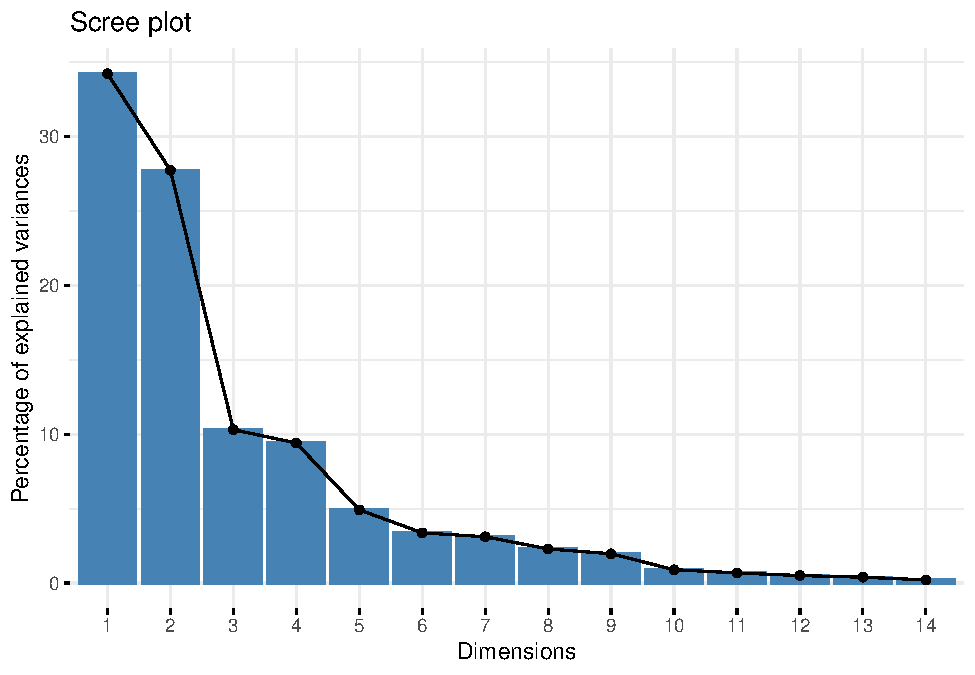
\includegraphics{bookdown-demo_files/figure-latex/0608-1.pdf}

\begin{Shaded}
\begin{Highlighting}[]
\KeywordTok{library}\NormalTok{(}\StringTok{"corrplot"}\NormalTok{)}
\KeywordTok{corrplot}\NormalTok{(res.pca}\OperatorTok{$}\NormalTok{var}\OperatorTok{$}\NormalTok{cos2, }\DataTypeTok{is.corr=}\OtherTok{FALSE}\NormalTok{, }\DataTypeTok{tl.cex =} \FloatTok{0.8}\NormalTok{)}
\end{Highlighting}
\end{Shaded}

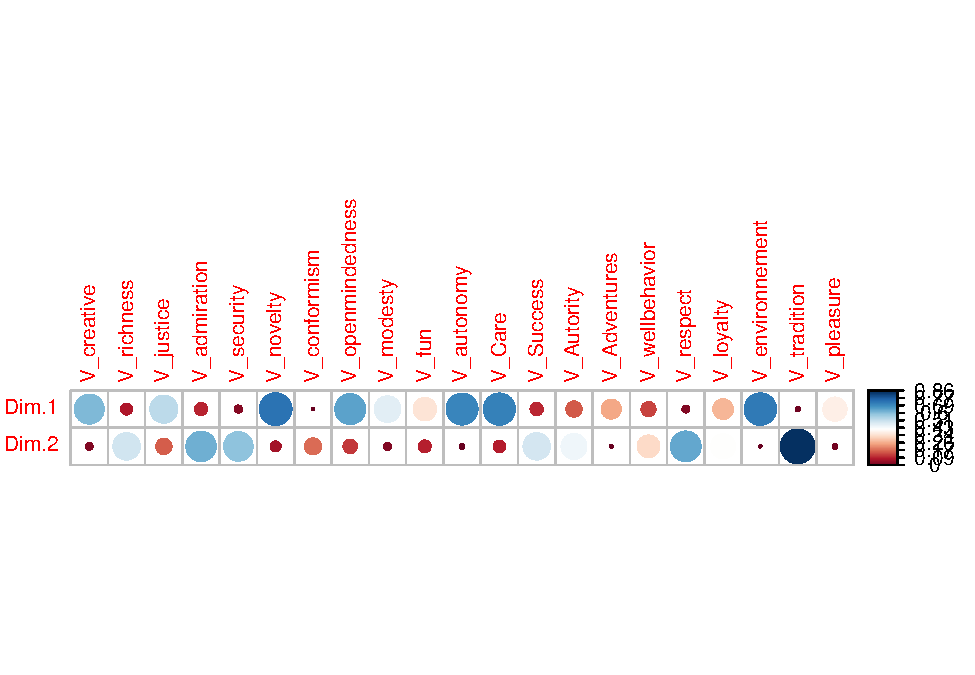
\includegraphics{bookdown-demo_files/figure-latex/0609-1.pdf}

\begin{Shaded}
\begin{Highlighting}[]
\KeywordTok{fviz_pca_var}\NormalTok{(res.pca, }\DataTypeTok{col.var =} \StringTok{"cos2"}\NormalTok{,}
             \DataTypeTok{gradient.cols =} \KeywordTok{c}\NormalTok{(}\StringTok{"#00AFBB"}\NormalTok{, }\StringTok{"#E7B800"}\NormalTok{, }\StringTok{"#FC4E07"}\NormalTok{),}
             \DataTypeTok{repel =} \OtherTok{TRUE} \CommentTok{# Évite le chevauchement de texte}
\NormalTok{             )}
\end{Highlighting}
\end{Shaded}

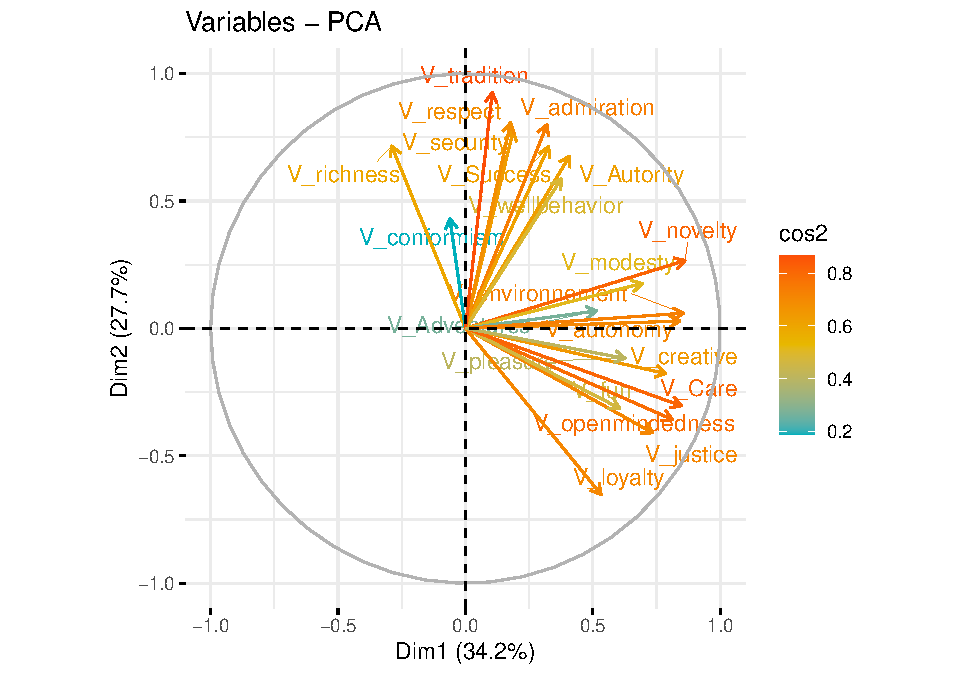
\includegraphics{bookdown-demo_files/figure-latex/0609-2.pdf}

\begin{Shaded}
\begin{Highlighting}[]
\KeywordTok{fviz_pca_ind}\NormalTok{(res.pca, }\DataTypeTok{col.ind =} \StringTok{"cos2"}\NormalTok{,}
             \DataTypeTok{gradient.cols =} \KeywordTok{c}\NormalTok{(}\StringTok{"#00AFBB"}\NormalTok{, }\StringTok{"#E7B800"}\NormalTok{, }\StringTok{"#FC4E07"}\NormalTok{),}
             \DataTypeTok{repel =} \OtherTok{TRUE} \CommentTok{# Évite le chevauchement de texte}
\NormalTok{             )}
\end{Highlighting}
\end{Shaded}

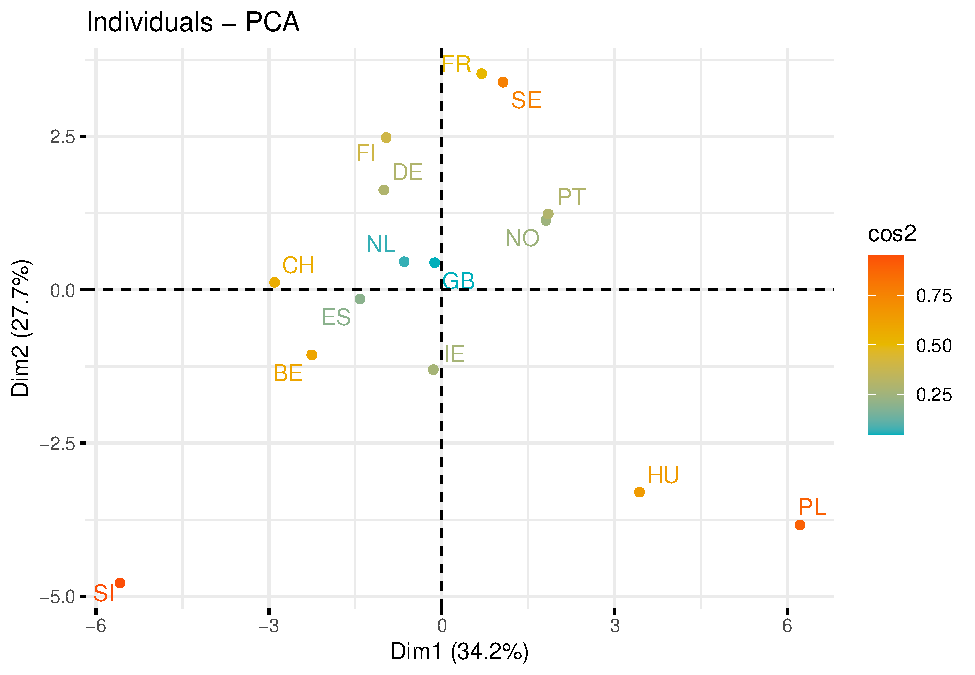
\includegraphics{bookdown-demo_files/figure-latex/0609-3.pdf}

\begin{Shaded}
\begin{Highlighting}[]
\CommentTok{### ce merveilleux bi plot}

\KeywordTok{fviz_pca_biplot}\NormalTok{(res.pca, }\DataTypeTok{col.ind =} \StringTok{"cos2"}\NormalTok{, }\DataTypeTok{labelsize =} \DecValTok{3}\NormalTok{,}
             \DataTypeTok{gradient.cols =} \KeywordTok{c}\NormalTok{(}\StringTok{"#00AFBB"}\NormalTok{, }\StringTok{"#E7B800"}\NormalTok{, }\StringTok{"#FC4E07"}\NormalTok{),}
             \DataTypeTok{repel =} \OtherTok{TRUE}\NormalTok{ )}\CommentTok{# Biplot des individus et variables}
\end{Highlighting}
\end{Shaded}

\includegraphics{bookdown-demo_files/figure-latex/0609-4.pdf}

\hypertarget{une-guxe9nuxe9ralisation-de-lacp-lafc}{%
\section{Une généralisation de l'ACP : l'AFC}\label{une-guxe9nuxe9ralisation-de-lacp-lafc}}

L'AFC trouve une application remarquable dans l'analyse de tableaux croisés. Elle est une méthode de réprésentation des profils lignes et colonnes:

On s'aperçoit que deux analyses peuvent être menées : l'une sur les colonnes, et l'autres sur les lignes. Dans les deux cas cette analyse peut se faire en comparant les colonnes (lignes) selon la formule suivante

\[
d_{i,j}= (f_{.i}-f_{.j})^2
\]
L'idée maintenant est claire : on mène deux acp, en ligne et en colonne, et on projettent conjointement ( dans un même espace)

\begin{Shaded}
\begin{Highlighting}[]
\KeywordTok{library}\NormalTok{(readr)}
\NormalTok{BDCOM_}\DecValTok{2020}\NormalTok{ <-}\StringTok{ }\KeywordTok{read_csv}\NormalTok{(}\StringTok{"Data//BDCOM/BDCOM_2020.csv"}\NormalTok{) }\OperatorTok\KeywordTok{rename}\NormalTok{(}\DataTypeTok{CODACT=}\NormalTok{CODE_ACTIVITE)}
\NormalTok{BDCOM_}\DecValTok{2017}\NormalTok{_CODACT_OD <-}\StringTok{ }\KeywordTok{read_delim}\NormalTok{(}\StringTok{"Data/BDCOM/BDCOM_2017_CODACT_OD.csv"}\NormalTok{, }
                                   \DataTypeTok{delim =} \StringTok{";"}\NormalTok{, }\DataTypeTok{escape_double =} \OtherTok{FALSE}\NormalTok{, }\DataTypeTok{trim_ws =} \OtherTok{TRUE}\NormalTok{)}

\NormalTok{df<-BDCOM_}\DecValTok{2020}\OperatorTok\KeywordTok{left_join}\NormalTok{(BDCOM_}\DecValTok{2017}\NormalTok{_CODACT_OD, }\DataTypeTok{by =} \StringTok{"CODACT"}\NormalTok{)}\OperatorTok\KeywordTok{rename}\NormalTok{(}\DataTypeTok{ACT=}\DecValTok{27}\NormalTok{)}
\NormalTok{t<-}\KeywordTok{table}\NormalTok{(df}\OperatorTok{$}\NormalTok{ARRONDISSEMENT,df}\OperatorTok{$}\NormalTok{ACT )}

\NormalTok{res.ca <-}\StringTok{ }\KeywordTok{CA}\NormalTok{(t, }
             \DataTypeTok{graph =} \OtherTok{TRUE}\NormalTok{)}
\end{Highlighting}
\end{Shaded}

\includegraphics{bookdown-demo_files/figure-latex/0610-1.pdf}

\begin{Shaded}
\begin{Highlighting}[]
\KeywordTok{plot}\NormalTok{(res.ca, }\DataTypeTok{autoLab =} \StringTok{"yes"}\NormalTok{)}
\end{Highlighting}
\end{Shaded}

\includegraphics{bookdown-demo_files/figure-latex/0610-2.pdf}

\begin{Shaded}
\begin{Highlighting}[]
\KeywordTok{fviz_ca_biplot}\NormalTok{(res.ca, }\DataTypeTok{labelsize =} \DecValTok{2}\NormalTok{, }\DataTypeTok{repel=}\OtherTok{TRUE}\NormalTok{)}\OperatorTok{+}
\StringTok{  }\KeywordTok{theme}\NormalTok{(}\DataTypeTok{text =} \KeywordTok{element_text}\NormalTok{(}\DataTypeTok{size =}\DecValTok{7}\NormalTok{)) }\OperatorTok{+}\KeywordTok{xlim}\NormalTok{(}\OperatorTok{-}\FloatTok{0.75}\NormalTok{, }\DecValTok{1}\NormalTok{)}\OperatorTok{+}\KeywordTok{ylim}\NormalTok{(}\OperatorTok{-}\NormalTok{.}\DecValTok{75}\NormalTok{,}\FloatTok{0.75}\NormalTok{)}
\end{Highlighting}
\end{Shaded}

\includegraphics{bookdown-demo_files/figure-latex/0610-3.pdf}

règle d'interprétation

\begin{itemize}
\tightlist
\item
  le point (0,0) représente le baycentre du nuage de point,et donc l'invidu moyens
\item
  les lignes/colonne les plus extcentrée sont les moins présentes, la distance d'une modalité d'une variable à une autres, indique la correspondance de ces deux modalités qui partagent les mêmes individus.
\item
  l'inertie total est chi²/n et donc une véritable méthode : analyse de la décomposition du khi2.
\end{itemize}

Dans notre exemple on note de suite les arrondissement 1 et 2 qui sont les plus proches de la catégorie commerce de gros.

On note aussi une disposition linéiaire qui opposent les arrondisssement excentré, aux arrondissement du centre. Un univers commercial résidentiel vs un univers de transit (spectacles et grands magasins)

\hypertarget{afcm-multiple}{%
\subsection{AFCM multiple}\label{afcm-multiple}}

Très rapidement la méthode a été appliquée à une généralisation des tableaux croisés : le tableau de burt, ou son équivalent : le tableau disjonctif complet.

exemple

La mise en oeuvre par factominer permet d'employer une techniques de représentation de variables complémentaires : elles n'interviennent pas dans le calcul de la configuration factorielles, mais leurs positions dans l'espace sont calculées comme le barycentre des individus qui possède le trait considéré. Leur projection a un rôle illustratif.

\begin{Shaded}
\begin{Highlighting}[]
\KeywordTok{library}\NormalTok{(FactoMineR)}
\KeywordTok{table}\NormalTok{(df}\OperatorTok{$}\NormalTok{ACT)}
\end{Highlighting}
\end{Shaded}

\begin{verbatim}
## 
##                        Agences                    Alimentaire 
##                           4240                           7663 
##                      Auto-Moto      Autres locaux en boutique 
##                            823                           9215 
##            Bricolage-Jardinage           Cafés et Restaurants 
##                            907                          15247 
##              Commerces de gros             Culture et loisirs 
##                           1009                           5289 
##        Equipement de la maison      Equipement de la personne 
##                           2666                           7324 
##                Grands magasins Hôtels et Auberges de jeunesse 
##                              9                           1894 
##                 Locaux vacants                        Médical 
##                           8761                           2094 
##                   Santé-Beauté       Services aux entreprises 
##                           2906                            535 
##      Services aux particuliers                     Spectacles 
##                          12453                            237
\end{verbatim}

\begin{Shaded}
\begin{Highlighting}[]
\NormalTok{foo<-df}\OperatorTok\StringTok{ }\NormalTok{dplyr}\OperatorTok{::}\KeywordTok{select}\NormalTok{(ACT, SURFACE, SITUATION, LIBACT, ARRONDISSEMENT)}\OperatorTok
\StringTok{  }\KeywordTok{as.matrix}\NormalTok{()}

\NormalTok{res<-}\KeywordTok{MCA}\NormalTok{(foo,}\DataTypeTok{graph =} \OtherTok{FALSE}\NormalTok{,}\DataTypeTok{quali.sup=}\DecValTok{5}\NormalTok{)}


\KeywordTok{fviz_mca_var}\NormalTok{(res, }\DataTypeTok{labelsize =} \DecValTok{2}\NormalTok{, }\DataTypeTok{repel=}\OtherTok{TRUE}\NormalTok{)}
\end{Highlighting}
\end{Shaded}

\includegraphics{bookdown-demo_files/figure-latex/0611-1.pdf}

remarques complémentaires :
* pas de signification de l'inertie globale qui dépend de la structure du tableau ( nombres de variables et de leurs modalités)

\hypertarget{duxe9veloppements}{%
\section{Développements}\label{duxe9veloppements}}

derrière les méthodes il y a un principe mathématique fondamental qui est au fondement de bien d'autres méthodes factorielles. C'est celle de la Singular Variance décomposition dont l'ACP est finalement un cas particulier.

\hypertarget{le-svd}{%
\subsection{le SVD}\label{le-svd}}

Le modèle mathématique fondamental

décomposer une matrice en plusieurs matrices
l'acp une application à une matrice de nature particulières : la matrice de covariance ou de corrélation si standardisée

de nombreuses autres applications :

\begin{itemize}
\tightlist
\item
  à des matrices de comptage
\item
  compression d'image
\item
  information retrieval
\end{itemize}

d'autres méthodes s'appuient sur ce principe fondamental, et permettent de traiter des données textuelle .

On repporte le lecteur au chapitre X de Booh NLP.

LSA
NFM

\hypertarget{acm-analyse-canonique-analyse-discriminante}{%
\subsection{ACM , analyse canonique , analyse discriminante}\label{acm-analyse-canonique-analyse-discriminante}}

Si ACP, AFC et AFCM ont pris le devant de la scène, bien d'autre méthodes analogues ont été développées

\begin{itemize}
\tightlist
\item
  ACM
\item
  Analyse canonique
\item
  Analyse factorielle discriminante qui a perdu du terrain au profit du modèle de régression logistique.
\end{itemize}

\hypertarget{en-conclusion}{%
\chapter{En conclusion}\label{en-conclusion}}

\begin{enumerate}
\def\labelenumi{\arabic{enumi})}
\item
  une idée essentielle : réduire de nombreuses variables à un petit jeu de variables synthétiques
\item
  des méthode au coeur de l'analyse des données
\item
  une autre idée essentielle : celle de vectoriser les données qu'on observe
\end{enumerate}

\hypertarget{clus}{%
\chapter{Clustering}\label{clus}}

L'objectif des méthodes de classification automatique est de regrouper des observations qui se ressemblent sur un ensemble multidimensionnel de caractéristiques.

insérer image

Dans ce chapitre nous examinons deux familles de méthodes qui le distingue par la procédure de calcul : hierarchique d'une part, non hiérarchique de l'autre. On garde pour le chapître suivant l'étude des modèles de décisions qui ont une longue et riche histoire en marketing et ont préparé le développement de certains modèles de machine learning.

\hypertarget{les-muxe9thodes-hiuxe9rarchiques-ascendantes}{%
\section{Les méthodes hiérarchiques ascendantes}\label{les-muxe9thodes-hiuxe9rarchiques-ascendantes}}

Elles trouvent leur origine en biologie où dès les années 1930 Sokal et Sneath\citep{sneath_numerical_1973} ont proposé des méthodes pour analyser l'évolution des espèces. L'idée réside dans la comparison de specimens sur la base d'un certains nombre de caractéristiques, d'abord des caractères phénotypiques, puis dans ce domaine en s'appuyant sur les caractéristiques génétiques. Nous n'entrerons pas dans une discussion plus approfondis mais signalons que ces choix déterminent des méthodes et des hypothèses très différentes et largement débattues (cladistique etc)

Prenons le cas de différences phénotypiques et le tableau suivant.

tableau

Le but du jeu est de regrouper successivement les spécimens en fonction de leur ressemblance. L'algorithme consiste simplement à 1) calculer toutes les ressemblances deux à deux et 2) à fondre en une classe les deux éléments qui se ressemble le plus. On réitère l'opération jusqu'à ce qu'on obtienne plus qu'une classe.

Le résultat est une arborescence dont chaque noeud représente un regrouppement de classe à un certain niveau de distance.

figure

Leurs variétés dépend de deux paramètres :

\begin{itemize}
\tightlist
\item
  le choix de la mesure de dissimilarités : Une distance euclidienne ? Son carré ? Une distance binaire comme l'indice de Jaccard?
\item
  le choix de la méthode d'agrégation : que choisit-on pour calculer la distance entre deux classes A et B : la plus grande des distances entre les éléments de A et ceux de B ? La plus petite ? La distance moyennes, la médiane ?
\end{itemize}

\hypertarget{mise-en-oeuvre}{%
\subsection{Mise en oeuvre}\label{mise-en-oeuvre}}

On utilise l'enquête d'happydemics sur la période de fin mars.

\begin{Shaded}
\begin{Highlighting}[]
\NormalTok{df<-}\KeywordTok{readRDS}\NormalTok{(}\StringTok{"./data/last.rds"}\NormalTok{) }\OperatorTok
\StringTok{  }\KeywordTok{filter}\NormalTok{(date2}\OperatorTok{>=}\KeywordTok{make_datetime}\NormalTok{(}\DataTypeTok{year=}\DecValTok{2022}\NormalTok{, }\DataTypeTok{month=}\DecValTok{3}\NormalTok{, }\DataTypeTok{day =} \DecValTok{19}\NormalTok{))}


\NormalTok{n_t<-}\KeywordTok{nrow}\NormalTok{(df)}

\NormalTok{period<-}\StringTok{" apres le 19 mars"}
\end{Highlighting}
\end{Shaded}

Il y a un trick de traitement des données. La question QCM a été encodée en une colonne, ajoutant les chaines de caractère des 16 thématiques avec un séparateurs \$ .

\begin{Shaded}
\begin{Highlighting}[]
\NormalTok{foo <-}\KeywordTok{as.data.frame}\NormalTok{(}\KeywordTok{str_split_fixed}\NormalTok{(df}\OperatorTok{$}\NormalTok{themes, }\StringTok{"}\CharTok{\textbackslash{}\textbackslash{}}\StringTok{$"}\NormalTok{,}\DataTypeTok{n=}\DecValTok{3}\NormalTok{)) }\CommentTok{# On splite la colonne thème en autant de thème possibles}

\NormalTok{foo1<-}\KeywordTok{cbind}\NormalTok{(df,foo)}\OperatorTok
\StringTok{  }\KeywordTok{rename}\NormalTok{(}\DataTypeTok{V1=}\DecValTok{23}\NormalTok{, }\DataTypeTok{V2=}\DecValTok{24}\NormalTok{, }\DataTypeTok{V3=}\DecValTok{25}\NormalTok{) }\OperatorTok
\StringTok{  }\NormalTok{dplyr}\OperatorTok{::}\KeywordTok{select}\NormalTok{(id,V1,V2,V3)}\OperatorTok\StringTok{ }
\StringTok{  }\KeywordTok{pivot_longer}\NormalTok{(}\OperatorTok{!}\NormalTok{id,}\DataTypeTok{names_to=}\StringTok{"rank"}\NormalTok{,}\DataTypeTok{values_to=}\StringTok{"theme"}\NormalTok{)}\OperatorTok\StringTok{ }
\StringTok{  }\KeywordTok{mutate}\NormalTok{(}\DataTypeTok{rank=}\KeywordTok{ifelse}\NormalTok{(rank}\OperatorTok{==}\StringTok{"V1"}\NormalTok{, }\DecValTok{3}\NormalTok{,}\KeywordTok{ifelse}\NormalTok{(rank}\OperatorTok{==}\StringTok{"V2"}\NormalTok{, }\DecValTok{2}\NormalTok{, }\KeywordTok{ifelse}\NormalTok{(rank}\OperatorTok{==}\StringTok{"V3"}\NormalTok{,}\DecValTok{1}\NormalTok{, }\DecValTok{0}\NormalTok{)))) }\OperatorTok\StringTok{ }\CommentTok{#on recode les rangs par un facteur d'importance de à 0 à 3}
\StringTok{  }\KeywordTok{filter}\NormalTok{(theme}\OperatorTok{!=}\StringTok{""}\NormalTok{)}\OperatorTok\StringTok{  }
\StringTok{  }\KeywordTok{mutate}\NormalTok{(}\DataTypeTok{theme=}\KeywordTok{str_trim}\NormalTok{(theme))}\OperatorTok
\StringTok{  }\KeywordTok{mutate}\NormalTok{(}\DataTypeTok{r=}\KeywordTok{as.numeric}\NormalTok{(rank))}\OperatorTok
\StringTok{  }\NormalTok{dplyr}\OperatorTok{::}\KeywordTok{select}\NormalTok{(}\OperatorTok{-}\NormalTok{rank)}


\NormalTok{n1<-}\KeywordTok{nrow}\NormalTok{(df) }\CommentTok{# le nombre d'individus}
\NormalTok{n2<-}\KeywordTok{nrow}\NormalTok{(foo1) }\CommentTok{#le nombre de mentions}
\end{Highlighting}
\end{Shaded}

Dans une première étape faisons le bilan global

\begin{Shaded}
\begin{Highlighting}[]
\CommentTok{#on calcule la proportion et la pénétration des items}

\NormalTok{foo2 <-foo1}\OperatorTok\StringTok{ }
\StringTok{  }\KeywordTok{mutate}\NormalTok{(}\DataTypeTok{m=}\DecValTok{1}\NormalTok{)}\OperatorTok
\StringTok{  }\KeywordTok{group_by}\NormalTok{(theme)}\OperatorTok
\StringTok{  }\KeywordTok{summarise}\NormalTok{(}\DataTypeTok{frequence=}\KeywordTok{sum}\NormalTok{(m),}
            \DataTypeTok{proportion=}\NormalTok{frequence}\OperatorTok{/}\NormalTok{n2,}
            \DataTypeTok{penetration=}\NormalTok{frequence}\OperatorTok{/}\NormalTok{n1)}


\NormalTok{col<-}\KeywordTok{c}\NormalTok{(}\StringTok{"#F1BB7B"}\NormalTok{,}
       \StringTok{"#FD6467"}\NormalTok{,}
       \StringTok{"#FD6467"}\NormalTok{,}
       \StringTok{"#FD6467"}\NormalTok{,}
       \StringTok{"#5B1A18"}\NormalTok{,}
       \StringTok{"#5B1A18"}\NormalTok{,}
       \StringTok{"#5B1A18"}\NormalTok{,}
       \StringTok{"#F1BB7B"}\NormalTok{,}
       \StringTok{"#FD6467"}\NormalTok{,}
       \StringTok{"#F1BB7B"}\NormalTok{,}
       \StringTok{"#F1BB7B"}\NormalTok{,}
       \StringTok{"#F1BB7B"}\NormalTok{,}
       \StringTok{"#F1BB7B"}\NormalTok{,}
       \StringTok{"#5B1A18"}\NormalTok{,}
       \StringTok{"#FD6467"}\NormalTok{,}
       \StringTok{"#F1BB7B"}\NormalTok{,}
       \StringTok{"#F1BB7B"}
\NormalTok{       )}

\NormalTok{brks<-}\KeywordTok{c}\NormalTok{(}\FloatTok{0.1}\NormalTok{, }\FloatTok{0.2}\NormalTok{, }\FloatTok{0.3}\NormalTok{,}\FloatTok{0.4}\NormalTok{,}\FloatTok{0.5}\NormalTok{,}\FloatTok{0.6}\NormalTok{)}
\KeywordTok{ggplot}\NormalTok{(foo2,}\KeywordTok{aes}\NormalTok{(}\DataTypeTok{x=}\KeywordTok{reorder}\NormalTok{(theme, frequence), }\DataTypeTok{y=}\NormalTok{penetration))}\OperatorTok{+}
\StringTok{  }\KeywordTok{geom_bar}\NormalTok{(}\DataTypeTok{stat=}\StringTok{"identity"}\NormalTok{, }\KeywordTok{aes}\NormalTok{(}\DataTypeTok{fill=}\NormalTok{theme))}\OperatorTok{+}
\StringTok{  }\KeywordTok{coord_flip}\NormalTok{()}\OperatorTok{+}
\StringTok{  }\KeywordTok{scale_fill_manual}\NormalTok{(}\DataTypeTok{values=}\NormalTok{col)}\OperatorTok{+}
\StringTok{  }\KeywordTok{labs}\NormalTok{(}\DataTypeTok{title =} \StringTok{"Pénétration des thèmes dans la population"}\NormalTok{,}
       \DataTypeTok{x=}\OtherTok{NULL}\NormalTok{, }
       \DataTypeTok{y=} \StringTok{"% de la population"}\NormalTok{, }
       \DataTypeTok{caption =} \StringTok{"data @happydemics dataviz @benavent"}\NormalTok{)}\OperatorTok{+}
\StringTok{  }\KeywordTok{theme_minimal}\NormalTok{()}\OperatorTok{+}
\StringTok{  }\KeywordTok{theme}\NormalTok{(}\DataTypeTok{legend.position =} \StringTok{"none"}\NormalTok{)}\OperatorTok{+}\StringTok{ }
\StringTok{  }\KeywordTok{scale_y_continuous}\NormalTok{(}\DataTypeTok{breaks =}\NormalTok{ brks, }\DataTypeTok{labels =}\NormalTok{ scales}\OperatorTok{::}\KeywordTok{percent}\NormalTok{(brks))}
\end{Highlighting}
\end{Shaded}

\includegraphics{bookdown-demo_files/figure-latex/0812-1.pdf}

\begin{Shaded}
\begin{Highlighting}[]
\KeywordTok{ggsave}\NormalTok{(}\KeywordTok{paste0}\NormalTok{(}\StringTok{"./plot/theme_"}\NormalTok{,period,}\StringTok{".jpg"}\NormalTok{),}\DataTypeTok{plot=}\KeywordTok{last_plot}\NormalTok{(), }\DataTypeTok{width =} \DecValTok{27}\NormalTok{, }\DataTypeTok{height =} \DecValTok{17}\NormalTok{, }\DataTypeTok{units =} \StringTok{"cm"}\NormalTok{)}
\end{Highlighting}
\end{Shaded}

\hypertarget{segmentation-simplifiuxe9e}{%
\section{segmentation simplifiée}\label{segmentation-simplifiuxe9e}}

On commence va reconstruire un tableaux des individus x les thèmes. On garde les rangs comme indicateurs de l'importance .

\begin{Shaded}
\begin{Highlighting}[]
\NormalTok{foo3<-foo1}\OperatorTok\StringTok{  }
\StringTok{  }\KeywordTok{pivot_wider}\NormalTok{(}\DataTypeTok{names_from=}\StringTok{"theme"}\NormalTok{, }\DataTypeTok{values_from=}\StringTok{"r"}\NormalTok{) }\OperatorTok
\StringTok{  }\KeywordTok{replace}\NormalTok{(}\KeywordTok{is.na}\NormalTok{(.), }\DecValTok{0}\NormalTok{)}
\KeywordTok{head}\NormalTok{(foo3, }\DecValTok{8}\NormalTok{)}
\end{Highlighting}
\end{Shaded}

\begin{verbatim}
## # A tibble: 8 x 17
##          id `L'immigration` `Le pouvoir d'achat` `L'éducation` `L'égalité Homm~`
##       <dbl>           <dbl>                <dbl>         <dbl>             <dbl>
## 1 235824277               3                    0             0                 0
## 2 235824417               0                    3             2                 1
## 3 235825307               0                    3             0                 0
## 4 235825503               0                    0             0                 0
## 5 235826269               0                    1             0                 0
## 6 235828154               0                    2             3                 0
## 7 235828507               0                    0             3                 2
## 8 235828613               1                    2             0                 0
## # ... with 12 more variables: `Les retraites` <dbl>, `L'environnement` <dbl>,
## #   `Le service public` <dbl>, `L'insécurité` <dbl>, `La santé` <dbl>,
## #   `Le chômage` <dbl>, `L'économie` <dbl>,
## #   `La science et la technologie` <dbl>, `L'identité nationale` <dbl>,
## #   `La sécurité nationale` <dbl>, `L'union Européenne` <dbl>,
## #   `La culture` <dbl>
\end{verbatim}

On calcule un tableau de distance et on performe la classification automatique. dans cet essai on tente un modèle à 8 groupes.

\begin{Shaded}
\begin{Highlighting}[]
\NormalTok{foo4<-foo3[,}\DecValTok{2}\OperatorTok{:}\DecValTok{17}\NormalTok{]}

\CommentTok{#distance}
\NormalTok{d<-}\KeywordTok{dist}\NormalTok{(foo4)}

\CommentTok{#clustering}
\NormalTok{h.D  <-}\StringTok{ }\KeywordTok{hclust}\NormalTok{(d, }\DataTypeTok{method=}\StringTok{"ward.D"}\NormalTok{)}

\CommentTok{#dendogramme}
\KeywordTok{plot}\NormalTok{(h.D,  }\DataTypeTok{hang=}\OperatorTok{-}\DecValTok{1}\NormalTok{)}

\CommentTok{#identification des clusters}
\KeywordTok{rect.hclust}\NormalTok{(h.D , }\DataTypeTok{k =} \DecValTok{8}\NormalTok{, }\DataTypeTok{border =} \DecValTok{2}\OperatorTok{:}\DecValTok{6}\NormalTok{)}
\end{Highlighting}
\end{Shaded}

\includegraphics{bookdown-demo_files/figure-latex/0814-1.pdf}

\begin{Shaded}
\begin{Highlighting}[]
\CommentTok{#attribution des clusters}
\NormalTok{memb <-}\StringTok{ }\KeywordTok{cutree}\NormalTok{(h.D, }\DataTypeTok{k =} \DecValTok{8}\NormalTok{)}

\CommentTok{#maj du fichier de données avec l'appartenace des individus aux groupes}
\NormalTok{foo5<-}\KeywordTok{cbind}\NormalTok{(foo4, memb)}
\end{Highlighting}
\end{Shaded}

Il reste à décrire les différents types sur les 16 variables qui les décrivent. On choisit une méthode de barre ordonnée avec un facetting par groupe.

\begin{Shaded}
\begin{Highlighting}[]
\NormalTok{foo6<-foo5 }\OperatorTok\StringTok{ }
\StringTok{  }\KeywordTok{group_by}\NormalTok{(memb) }\OperatorTok
\StringTok{  }\KeywordTok{pivot_longer}\NormalTok{(}\OperatorTok{-}\NormalTok{memb,}\DataTypeTok{names_to=}\StringTok{"Thèmes"}\NormalTok{,}\DataTypeTok{values_to=}\StringTok{"Valeurs"}\NormalTok{)}\OperatorTok
\StringTok{  }\KeywordTok{group_by}\NormalTok{(memb,Thèmes)}\OperatorTok
\StringTok{  }\KeywordTok{summarise}\NormalTok{(}\DataTypeTok{Valeurs=}\KeywordTok{mean}\NormalTok{(Valeurs))}

\NormalTok{foo6}\OperatorTok{$}\NormalTok{group[foo6}\OperatorTok{$}\NormalTok{memb}\OperatorTok{==}\DecValTok{1}\NormalTok{]<-}\StringTok{"multicritère"}
\NormalTok{foo6}\OperatorTok{$}\NormalTok{group[foo6}\OperatorTok{$}\NormalTok{memb}\OperatorTok{==}\DecValTok{2}\NormalTok{]<-}\StringTok{"Santé/Educ"}
\NormalTok{foo6}\OperatorTok{$}\NormalTok{group[foo6}\OperatorTok{$}\NormalTok{memb}\OperatorTok{==}\DecValTok{3}\NormalTok{]<-}\StringTok{"Pouvoir d'achat/nretraites"}
\NormalTok{foo6}\OperatorTok{$}\NormalTok{group[foo6}\OperatorTok{$}\NormalTok{memb}\OperatorTok{==}\DecValTok{5}\NormalTok{]<-}\StringTok{"Immigration/nInsécurité "}
\NormalTok{foo6}\OperatorTok{$}\NormalTok{group[foo6}\OperatorTok{$}\NormalTok{memb}\OperatorTok{==}\DecValTok{4}\NormalTok{]<-}\StringTok{"égalité h/F"}
\NormalTok{foo6}\OperatorTok{$}\NormalTok{group[foo6}\OperatorTok{$}\NormalTok{memb}\OperatorTok{==}\DecValTok{6}\NormalTok{]<-}\StringTok{"Pouvoir d'achat/nSanté"}
\NormalTok{foo6}\OperatorTok{$}\NormalTok{group[foo6}\OperatorTok{$}\NormalTok{memb}\OperatorTok{==}\DecValTok{7}\NormalTok{]<-}\StringTok{"Economie"}
\NormalTok{foo6}\OperatorTok{$}\NormalTok{group[foo6}\OperatorTok{$}\NormalTok{memb}\OperatorTok{==}\DecValTok{8}\NormalTok{]<-}\StringTok{"Environnement"}

\KeywordTok{library}\NormalTok{(scales)}
\NormalTok{brks<-}\KeywordTok{c}\NormalTok{(}\FloatTok{0.5}\NormalTok{,}\DecValTok{1}\NormalTok{,}\FloatTok{1.5}\NormalTok{,}\DecValTok{2}\NormalTok{, }\FloatTok{2.5}\NormalTok{,}\DecValTok{3}\NormalTok{)}
\NormalTok{p2<-}\StringTok{ }\KeywordTok{ggplot}\NormalTok{(foo6, }\KeywordTok{aes}\NormalTok{(}\DataTypeTok{x=}\KeywordTok{reorder}\NormalTok{(Thèmes, Valeurs), }\DataTypeTok{y=}\NormalTok{Valeurs))}\OperatorTok{+}
\StringTok{  }\KeywordTok{geom_bar}\NormalTok{(}\DataTypeTok{stat=}\StringTok{"identity"}\NormalTok{,}\KeywordTok{aes}\NormalTok{(}\DataTypeTok{fill=}\KeywordTok{as.factor}\NormalTok{(Thèmes)))}\OperatorTok{+}
\StringTok{  }\KeywordTok{facet_wrap}\NormalTok{(}\KeywordTok{vars}\NormalTok{(memb), }\DataTypeTok{ncol=}\DecValTok{4}\NormalTok{)}\OperatorTok{+}
\StringTok{  }\KeywordTok{coord_flip}\NormalTok{()}\OperatorTok{+}
\StringTok{  }\KeywordTok{scale_fill_manual}\NormalTok{(}\DataTypeTok{values=}\NormalTok{col)}\OperatorTok{+}
\StringTok{  }\KeywordTok{theme_minimal}\NormalTok{()}\OperatorTok{+}
\StringTok{  }\KeywordTok{scale_y_continuous}\NormalTok{(}\DataTypeTok{breaks=}\NormalTok{brks)}\OperatorTok{+}\StringTok{ }
\StringTok{  }\KeywordTok{theme}\NormalTok{(}\DataTypeTok{legend.position =} \StringTok{"none"}\NormalTok{, }\DataTypeTok{axis.text=}\KeywordTok{element_text}\NormalTok{(}\DataTypeTok{size=}\DecValTok{7}\NormalTok{),}\DataTypeTok{axis.text.x=}\KeywordTok{element_text}\NormalTok{(}\DataTypeTok{angle =} \DecValTok{45}\NormalTok{, }\DataTypeTok{vjust =} \FloatTok{0.5}\NormalTok{, }\DataTypeTok{size=}\DecValTok{2}\NormalTok{))}\OperatorTok{+}\StringTok{ }
\StringTok{  }\KeywordTok{labs}\NormalTok{(}\DataTypeTok{title =} \StringTok{"Profils des segments}\CharTok{\textbackslash{}n}\StringTok{par importance des thématiques"}\NormalTok{, }\DataTypeTok{x=}\OtherTok{NULL}\NormalTok{, }\DataTypeTok{y=}\StringTok{"importance moyenne (de 0 à 3)"}\NormalTok{) }

\NormalTok{p2}
\end{Highlighting}
\end{Shaded}

\includegraphics{bookdown-demo_files/figure-latex/0815-1.pdf}

\begin{Shaded}
\begin{Highlighting}[]
\KeywordTok{library}\NormalTok{(wesanderson)}
\NormalTok{seg_col<-}\KeywordTok{wes_palette}\NormalTok{(}\StringTok{"Zissou1"}\NormalTok{, }\DecValTok{8}\NormalTok{, }\DataTypeTok{type =} \StringTok{"continuous"}\NormalTok{)}
\NormalTok{n<-}\KeywordTok{nrow}\NormalTok{(foo5)}
\NormalTok{foo6<-foo5 }\OperatorTok\StringTok{ }\KeywordTok{mutate}\NormalTok{(}\DataTypeTok{n=}\DecValTok{1}\NormalTok{) }\OperatorTok
\StringTok{  }\KeywordTok{group_by}\NormalTok{(memb)}\OperatorTok
\StringTok{  }\KeywordTok{summarise}\NormalTok{(}\DataTypeTok{freq=}\KeywordTok{sum}\NormalTok{(n, }\DataTypeTok{na.rm=}\OtherTok{TRUE}\NormalTok{))}\OperatorTok\StringTok{ }\KeywordTok{mutate}\NormalTok{( }\DataTypeTok{freq=}\NormalTok{freq}\OperatorTok{/}\NormalTok{n)}


\NormalTok{foo6}\OperatorTok{$}\NormalTok{group[foo6}\OperatorTok{$}\NormalTok{memb}\OperatorTok{==}\DecValTok{1}\NormalTok{]<-}\StringTok{"multicritère"}
\NormalTok{foo6}\OperatorTok{$}\NormalTok{group[foo6}\OperatorTok{$}\NormalTok{memb}\OperatorTok{==}\DecValTok{2}\NormalTok{]<-}\StringTok{"Santé/Educ"}
\NormalTok{foo6}\OperatorTok{$}\NormalTok{group[foo6}\OperatorTok{$}\NormalTok{memb}\OperatorTok{==}\DecValTok{3}\NormalTok{]<-}\StringTok{"Pouvoir d'achat/nretraites"}
\NormalTok{foo6}\OperatorTok{$}\NormalTok{group[foo6}\OperatorTok{$}\NormalTok{memb}\OperatorTok{==}\DecValTok{5}\NormalTok{]<-}\StringTok{"Immigration/nInsécurité "}
\NormalTok{foo6}\OperatorTok{$}\NormalTok{group[foo6}\OperatorTok{$}\NormalTok{memb}\OperatorTok{==}\DecValTok{4}\NormalTok{]<-}\StringTok{"égalité h/F"}
\NormalTok{foo6}\OperatorTok{$}\NormalTok{group[foo6}\OperatorTok{$}\NormalTok{memb}\OperatorTok{==}\DecValTok{6}\NormalTok{]<-}\StringTok{"Pouvoir d'achat/nSanté"}
\NormalTok{foo6}\OperatorTok{$}\NormalTok{group[foo6}\OperatorTok{$}\NormalTok{memb}\OperatorTok{==}\DecValTok{7}\NormalTok{]<-}\StringTok{"Economie"}
\NormalTok{foo6}\OperatorTok{$}\NormalTok{group[foo6}\OperatorTok{$}\NormalTok{memb}\OperatorTok{==}\DecValTok{8}\NormalTok{]<-}\StringTok{"Environnement"}


\NormalTok{p1<-}\StringTok{ }\KeywordTok{ggplot}\NormalTok{(foo6, }\KeywordTok{aes}\NormalTok{(}\DataTypeTok{x=}\NormalTok{group, }\DataTypeTok{y=}\NormalTok{freq))}\OperatorTok{+}
\StringTok{  }\KeywordTok{geom_bar}\NormalTok{(}\DataTypeTok{stat=}\StringTok{"identity"}\NormalTok{, }\KeywordTok{aes}\NormalTok{(}\DataTypeTok{fill=}\NormalTok{group))}\OperatorTok{+}
\StringTok{  }\KeywordTok{scale_fill_manual}\NormalTok{(}\DataTypeTok{values=}\NormalTok{seg_col) }\OperatorTok{+}\StringTok{ }
\StringTok{  }\KeywordTok{theme_minimal}\NormalTok{()}\OperatorTok{+}\StringTok{ }
\StringTok{  }\KeywordTok{labs}\NormalTok{(}\DataTypeTok{title=}\StringTok{"Poids des segments"}\NormalTok{, }\DataTypeTok{x=}\OtherTok{NULL}\NormalTok{, }\DataTypeTok{y=}\StringTok{"Proportion"}\NormalTok{)}\OperatorTok{+}\StringTok{  }
\StringTok{  }\KeywordTok{scale_y_continuous}\NormalTok{(}\DataTypeTok{breaks=}\NormalTok{brks,}\DataTypeTok{labels=}\NormalTok{percent)}\OperatorTok{+}\StringTok{  }
\StringTok{  }\KeywordTok{theme}\NormalTok{(}\DataTypeTok{legend.position =} \StringTok{"none"}\NormalTok{)}

\KeywordTok{plot_grid}\NormalTok{(p1, p2, }\DataTypeTok{labels =} \KeywordTok{c}\NormalTok{(}\StringTok{'A'}\NormalTok{, }\StringTok{'B'}\NormalTok{), }\DataTypeTok{label_size =} \DecValTok{12}\NormalTok{, }\DataTypeTok{ncol=}\DecValTok{1}\NormalTok{,}\DataTypeTok{rel_heights =}  \KeywordTok{c}\NormalTok{(}\DecValTok{1}\NormalTok{, }\DecValTok{2}\NormalTok{))}
\end{Highlighting}
\end{Shaded}

\includegraphics{bookdown-demo_files/figure-latex/0815-2.pdf}

\begin{Shaded}
\begin{Highlighting}[]
\KeywordTok{ggsave}\NormalTok{(}\StringTok{"./plot/g_segment.jpg"}\NormalTok{,}\DataTypeTok{plot=}\KeywordTok{last_plot}\NormalTok{(), }\DataTypeTok{width =} \DecValTok{27}\NormalTok{, }\DataTypeTok{height =} \DecValTok{17}\NormalTok{, }\DataTypeTok{units =} \StringTok{"cm"}\NormalTok{)}
\end{Highlighting}
\end{Shaded}

\hypertarget{tableaux-croisuxe9s-de-la-typologie-et-des-crituxe8res-sociaux-duxe9mos}{%
\section{tableaux croisés de la typologie et des critères sociaux démos}\label{tableaux-croisuxe9s-de-la-typologie-et-des-crituxe8res-sociaux-duxe9mos}}

On revient à une approche descriptive, on croisant successivement notre variable typologie avec les critères socio-demo qui ont été mesurés dans l'enquête.

( une boucle simplifierait ! )

\begin{Shaded}
\begin{Highlighting}[]
\NormalTok{df<-}\KeywordTok{cbind}\NormalTok{(df,foo5)}

\NormalTok{df}\OperatorTok{$}\NormalTok{group[df}\OperatorTok{$}\NormalTok{memb}\OperatorTok{==}\DecValTok{1}\NormalTok{]<-}\StringTok{"multicritère"}
\NormalTok{df}\OperatorTok{$}\NormalTok{group[df}\OperatorTok{$}\NormalTok{memb}\OperatorTok{==}\DecValTok{2}\NormalTok{]<-}\StringTok{"Santé/Educ"}
\NormalTok{df}\OperatorTok{$}\NormalTok{group[df}\OperatorTok{$}\NormalTok{memb}\OperatorTok{==}\DecValTok{3}\NormalTok{]<-}\StringTok{"Pouvoir d'achat/nretraites"}
\NormalTok{df}\OperatorTok{$}\NormalTok{group[df}\OperatorTok{$}\NormalTok{memb}\OperatorTok{==}\DecValTok{5}\NormalTok{]<-}\StringTok{"Immigration/nInsécurité "}
\NormalTok{df}\OperatorTok{$}\NormalTok{group[df}\OperatorTok{$}\NormalTok{memb}\OperatorTok{==}\DecValTok{4}\NormalTok{]<-}\StringTok{"égalité h/F"}
\NormalTok{df}\OperatorTok{$}\NormalTok{group[df}\OperatorTok{$}\NormalTok{memb}\OperatorTok{==}\DecValTok{6}\NormalTok{]<-}\StringTok{"Pouvoir d'achat/nSanté"}
\NormalTok{df}\OperatorTok{$}\NormalTok{group[df}\OperatorTok{$}\NormalTok{memb}\OperatorTok{==}\DecValTok{7}\NormalTok{]<-}\StringTok{"Economie"}
\NormalTok{df}\OperatorTok{$}\NormalTok{group[df}\OperatorTok{$}\NormalTok{memb}\OperatorTok{==}\DecValTok{8}\NormalTok{]<-}\StringTok{"Environnement"}


\NormalTok{foo<-df }\OperatorTok\StringTok{ }
\StringTok{  }\KeywordTok{group_by}\NormalTok{(group, Sensibilité) }\OperatorTok\StringTok{ }
\StringTok{   }\KeywordTok{summarize}\NormalTok{(}\DataTypeTok{n=}\KeywordTok{n}\NormalTok{())}\OperatorTok
\StringTok{  }\KeywordTok{mutate}\NormalTok{(}\DataTypeTok{prop=}\KeywordTok{round}\NormalTok{(n}\OperatorTok{/}\KeywordTok{sum}\NormalTok{(n),}\DecValTok{3}\NormalTok{), }\DataTypeTok{cum=}\DecValTok{1} \OperatorTok{-}\StringTok{ }\NormalTok{(}\KeywordTok{cumsum}\NormalTok{(prop)}\OperatorTok{-}\NormalTok{prop}\OperatorTok{/}\DecValTok{2}\NormalTok{))}

\NormalTok{g01<-}\KeywordTok{ggplot}\NormalTok{(foo,}\KeywordTok{aes}\NormalTok{(}\DataTypeTok{x=}\NormalTok{group, }\DataTypeTok{y=}\NormalTok{prop, }\DataTypeTok{group=}\NormalTok{Sensibilité))}\OperatorTok{+}
\StringTok{  }\KeywordTok{geom_bar}\NormalTok{(}\DataTypeTok{stat=}\StringTok{"identity"}\NormalTok{,}\KeywordTok{aes}\NormalTok{(}\DataTypeTok{y =}\NormalTok{ prop, }\DataTypeTok{fill=}\NormalTok{Sensibilité)) }\OperatorTok{+}\StringTok{ }
\StringTok{ }\KeywordTok{scale_y_continuous}\NormalTok{(}\DataTypeTok{breaks =}\NormalTok{ brks, }\DataTypeTok{labels =}\NormalTok{ scales}\OperatorTok{::}\KeywordTok{percent}\NormalTok{(brks)) }\OperatorTok{+}
\StringTok{  }\KeywordTok{scale_fill_manual}\NormalTok{(}\DataTypeTok{values=}\NormalTok{SensiP2) }\OperatorTok{+}\StringTok{ }
\StringTok{  }\KeywordTok{geom_text}\NormalTok{(}\KeywordTok{aes}\NormalTok{(}\DataTypeTok{label =}\NormalTok{ prop, }\DataTypeTok{y=}\NormalTok{cum),}\DataTypeTok{size=}\DecValTok{2}\NormalTok{,}\DataTypeTok{color=}\StringTok{"white"}\NormalTok{, }\DataTypeTok{vjust =} \FloatTok{0.5}\NormalTok{)}\OperatorTok{+}
\StringTok{  }\KeywordTok{coord_flip}\NormalTok{()}\OperatorTok{+}
\StringTok{  }\KeywordTok{labs}\NormalTok{(}\DataTypeTok{title =} \StringTok{"Types d'attentes par sensibilité politique "}\NormalTok{, }
       \DataTypeTok{x=}\OtherTok{NULL}\NormalTok{, }\DataTypeTok{y=}\OtherTok{NULL}\NormalTok{,)}\OperatorTok{+}
\StringTok{  }\KeywordTok{theme_bw}\NormalTok{()}\OperatorTok{+}\StringTok{  }\KeywordTok{theme}\NormalTok{(}\DataTypeTok{axis.text.x =} \KeywordTok{element_text}\NormalTok{(}\DataTypeTok{size =} \DecValTok{7}\NormalTok{), }\DataTypeTok{legend.text =} \KeywordTok{element_text}\NormalTok{(}\DataTypeTok{size =} \DecValTok{7}\NormalTok{)) }



\KeywordTok{ggsave}\NormalTok{(}\StringTok{"./plot/g_segment01.jpg"}\NormalTok{,}\DataTypeTok{plot=}\KeywordTok{last_plot}\NormalTok{(), }\DataTypeTok{width =} \DecValTok{27}\NormalTok{, }\DataTypeTok{height =} \DecValTok{17}\NormalTok{, }\DataTypeTok{units =} \StringTok{"cm"}\NormalTok{)}


\NormalTok{foo<-df }\OperatorTok\StringTok{ }
\StringTok{  }\KeywordTok{group_by}\NormalTok{(group, Age) }\OperatorTok\StringTok{ }
\StringTok{   }\KeywordTok{summarize}\NormalTok{(}\DataTypeTok{n=}\KeywordTok{n}\NormalTok{())}\OperatorTok
\StringTok{  }\KeywordTok{mutate}\NormalTok{(}\DataTypeTok{prop=}\KeywordTok{round}\NormalTok{(n}\OperatorTok{/}\KeywordTok{sum}\NormalTok{(n),}\DecValTok{3}\NormalTok{), }\DataTypeTok{cum=}\DecValTok{1} \OperatorTok{-}\StringTok{ }\NormalTok{(}\KeywordTok{cumsum}\NormalTok{(prop)}\OperatorTok{-}\NormalTok{prop}\OperatorTok{/}\DecValTok{2}\NormalTok{))}

\NormalTok{g02<-}\KeywordTok{ggplot}\NormalTok{(foo,}\KeywordTok{aes}\NormalTok{(}\DataTypeTok{x=}\NormalTok{group, }\DataTypeTok{y=}\NormalTok{prop, }\DataTypeTok{group=}\NormalTok{Age))}\OperatorTok{+}
\StringTok{  }\KeywordTok{geom_bar}\NormalTok{(}\DataTypeTok{stat=}\StringTok{"identity"}\NormalTok{,}\KeywordTok{aes}\NormalTok{(}\DataTypeTok{y =}\NormalTok{ prop, }\DataTypeTok{fill=}\NormalTok{Age)) }\OperatorTok{+}\StringTok{ }
\StringTok{ }\KeywordTok{scale_y_continuous}\NormalTok{(}\DataTypeTok{breaks =}\NormalTok{ brks, }\DataTypeTok{labels =}\NormalTok{ scales}\OperatorTok{::}\KeywordTok{percent}\NormalTok{(brks)) }\OperatorTok{+}
\StringTok{  }\KeywordTok{scale_fill_brewer}\NormalTok{(}\DataTypeTok{palette=}\StringTok{"Spectral"}\NormalTok{) }\OperatorTok{+}\StringTok{ }\KeywordTok{geom_text}\NormalTok{(}\KeywordTok{aes}\NormalTok{(}\DataTypeTok{label =}\NormalTok{ prop, }\DataTypeTok{y=}\NormalTok{cum),}\DataTypeTok{size=}\DecValTok{2}\NormalTok{,}\DataTypeTok{color=}\StringTok{"white"}\NormalTok{, }\DataTypeTok{vjust =} \FloatTok{0.5}\NormalTok{)}\OperatorTok{+}
\StringTok{  }\KeywordTok{coord_flip}\NormalTok{()}\OperatorTok{+}
\StringTok{  }\KeywordTok{labs}\NormalTok{(}\DataTypeTok{title =} \StringTok{"Types d'attentes par classe d'âge "}\NormalTok{, }
       \DataTypeTok{x=}\OtherTok{NULL}\NormalTok{, }\DataTypeTok{y=}\OtherTok{NULL}\NormalTok{,)}\OperatorTok{+}\KeywordTok{theme_bw}\NormalTok{()  }\OperatorTok{+}
\StringTok{  }\KeywordTok{theme}\NormalTok{(}\DataTypeTok{axis.text.x =} \KeywordTok{element_text}\NormalTok{(}\DataTypeTok{size =} \DecValTok{7}\NormalTok{), }\DataTypeTok{legend.text =} \KeywordTok{element_text}\NormalTok{(}\DataTypeTok{size =} \DecValTok{7}\NormalTok{)) }



\KeywordTok{ggsave}\NormalTok{(}\StringTok{"./plot/g_segment02.jpg"}\NormalTok{,}\DataTypeTok{plot=}\KeywordTok{last_plot}\NormalTok{(), }\DataTypeTok{width =} \DecValTok{27}\NormalTok{, }\DataTypeTok{height =} \DecValTok{17}\NormalTok{, }\DataTypeTok{units =} \StringTok{"cm"}\NormalTok{)}


\NormalTok{foo<-df }\OperatorTok\StringTok{ }
\StringTok{  }\KeywordTok{group_by}\NormalTok{(group, Sexe) }\OperatorTok\StringTok{ }
\StringTok{   }\KeywordTok{summarize}\NormalTok{(}\DataTypeTok{n=}\KeywordTok{n}\NormalTok{())}\OperatorTok
\StringTok{  }\KeywordTok{mutate}\NormalTok{(}\DataTypeTok{prop=}\KeywordTok{round}\NormalTok{(n}\OperatorTok{/}\KeywordTok{sum}\NormalTok{(n),}\DecValTok{3}\NormalTok{), }\DataTypeTok{cum=}\DecValTok{1} \OperatorTok{-}\StringTok{ }\NormalTok{(}\KeywordTok{cumsum}\NormalTok{(prop)}\OperatorTok{-}\NormalTok{prop}\OperatorTok{/}\DecValTok{2}\NormalTok{))}

\NormalTok{g03<-}\KeywordTok{ggplot}\NormalTok{(foo,}\KeywordTok{aes}\NormalTok{(}\DataTypeTok{x=}\NormalTok{group, }\DataTypeTok{y=}\NormalTok{prop, }\DataTypeTok{group=}\NormalTok{Sexe))}\OperatorTok{+}
\StringTok{  }\KeywordTok{geom_bar}\NormalTok{(}\DataTypeTok{stat=}\StringTok{"identity"}\NormalTok{,}\KeywordTok{aes}\NormalTok{(}\DataTypeTok{y =}\NormalTok{ prop, }\DataTypeTok{fill=}\NormalTok{Sexe)) }\OperatorTok{+}\StringTok{ }
\StringTok{ }\KeywordTok{scale_y_continuous}\NormalTok{(}\DataTypeTok{breaks =}\NormalTok{ brks, }\DataTypeTok{labels =}\NormalTok{ scales}\OperatorTok{::}\KeywordTok{percent}\NormalTok{(brks)) }\OperatorTok{+}
\StringTok{  }\KeywordTok{scale_fill_brewer}\NormalTok{(}\DataTypeTok{palette=}\StringTok{"Spectral"}\NormalTok{) }\OperatorTok{+}\StringTok{ }\KeywordTok{geom_text}\NormalTok{(}\KeywordTok{aes}\NormalTok{(}\DataTypeTok{label =}\NormalTok{ prop, }\DataTypeTok{y=}\NormalTok{cum),}\DataTypeTok{size=}\DecValTok{2}\NormalTok{,}\DataTypeTok{color=}\StringTok{"white"}\NormalTok{, }\DataTypeTok{vjust =} \FloatTok{0.5}\NormalTok{)}\OperatorTok{+}
\StringTok{  }\KeywordTok{coord_flip}\NormalTok{()}\OperatorTok{+}\StringTok{  }\KeywordTok{theme_bw}\NormalTok{()}\OperatorTok{+}
\StringTok{  }\KeywordTok{labs}\NormalTok{(}\DataTypeTok{title =} \StringTok{"Types d'attentes par genre "}\NormalTok{, }
       \DataTypeTok{x=}\OtherTok{NULL}\NormalTok{, }\DataTypeTok{y=}\OtherTok{NULL}\NormalTok{,)}\OperatorTok{+}
\StringTok{  }\KeywordTok{theme}\NormalTok{(}\DataTypeTok{axis.text.x =} \KeywordTok{element_text}\NormalTok{(}\DataTypeTok{size =} \DecValTok{7}\NormalTok{), }\DataTypeTok{legend.text =} \KeywordTok{element_text}\NormalTok{(}\DataTypeTok{size =} \DecValTok{7}\NormalTok{))}

\KeywordTok{ggsave}\NormalTok{(}\StringTok{"./plot/g_segment03.jpg"}\NormalTok{,}\DataTypeTok{plot=}\KeywordTok{last_plot}\NormalTok{(), }\DataTypeTok{width =} \DecValTok{27}\NormalTok{, }\DataTypeTok{height =} \DecValTok{17}\NormalTok{, }\DataTypeTok{units =} \StringTok{"cm"}\NormalTok{)}

\NormalTok{foo<-df }\OperatorTok\StringTok{ }
\StringTok{  }\KeywordTok{group_by}\NormalTok{(group, Education) }\OperatorTok\StringTok{ }
\StringTok{   }\KeywordTok{summarize}\NormalTok{(}\DataTypeTok{n=}\KeywordTok{n}\NormalTok{())}\OperatorTok
\StringTok{  }\KeywordTok{mutate}\NormalTok{(}\DataTypeTok{prop=}\KeywordTok{round}\NormalTok{(n}\OperatorTok{/}\KeywordTok{sum}\NormalTok{(n),}\DecValTok{3}\NormalTok{), }\DataTypeTok{cum=}\DecValTok{1} \OperatorTok{-}\StringTok{ }\NormalTok{(}\KeywordTok{cumsum}\NormalTok{(prop)}\OperatorTok{-}\NormalTok{prop}\OperatorTok{/}\DecValTok{2}\NormalTok{))}

\NormalTok{g04<-}\KeywordTok{ggplot}\NormalTok{(foo,}\KeywordTok{aes}\NormalTok{(}\DataTypeTok{x=}\NormalTok{group, }\DataTypeTok{y=}\NormalTok{prop, }\DataTypeTok{group=}\NormalTok{Education))}\OperatorTok{+}
\StringTok{  }\KeywordTok{geom_bar}\NormalTok{(}\DataTypeTok{stat=}\StringTok{"identity"}\NormalTok{,}\KeywordTok{aes}\NormalTok{(}\DataTypeTok{y =}\NormalTok{ prop, }\DataTypeTok{fill=}\NormalTok{Education)) }\OperatorTok{+}\StringTok{ }
\StringTok{ }\KeywordTok{scale_y_continuous}\NormalTok{(}\DataTypeTok{breaks =}\NormalTok{ brks, }\DataTypeTok{labels =}\NormalTok{ scales}\OperatorTok{::}\KeywordTok{percent}\NormalTok{(brks)) }\OperatorTok{+}
\StringTok{  }\KeywordTok{scale_fill_brewer}\NormalTok{(}\DataTypeTok{palette=}\StringTok{"Spectral"}\NormalTok{) }\OperatorTok{+}\StringTok{ }
\StringTok{  }\KeywordTok{geom_text}\NormalTok{(}\KeywordTok{aes}\NormalTok{(}\DataTypeTok{label =}\NormalTok{ prop, }\DataTypeTok{y=}\NormalTok{cum),}\DataTypeTok{size=}\FloatTok{1.5}\NormalTok{,}\DataTypeTok{color=}\StringTok{"white"}\NormalTok{, }\DataTypeTok{vjust =} \FloatTok{0.5}\NormalTok{)}\OperatorTok{+}
\StringTok{  }\KeywordTok{coord_flip}\NormalTok{()}\OperatorTok{+}\KeywordTok{theme_bw}\NormalTok{()}\OperatorTok{+}
\StringTok{  }\KeywordTok{labs}\NormalTok{(}\DataTypeTok{title =} \StringTok{"Types d'attentes par niveau d'éducation "}\NormalTok{, }
       \DataTypeTok{x=}\OtherTok{NULL}\NormalTok{, }\DataTypeTok{y=}\OtherTok{NULL}\NormalTok{,)}\OperatorTok{+}
\StringTok{  }\KeywordTok{theme}\NormalTok{(}\DataTypeTok{axis.text.x =} \KeywordTok{element_text}\NormalTok{(}\DataTypeTok{size =} \DecValTok{7}\NormalTok{), }\DataTypeTok{legend.text =} \KeywordTok{element_text}\NormalTok{(}\DataTypeTok{size =} \DecValTok{7}\NormalTok{)) }
  


\KeywordTok{ggsave}\NormalTok{(}\StringTok{"./plot/g_segment04.jpg"}\NormalTok{,}\DataTypeTok{plot=}\KeywordTok{last_plot}\NormalTok{(), }\DataTypeTok{width =} \DecValTok{27}\NormalTok{, }\DataTypeTok{height =} \DecValTok{17}\NormalTok{, }\DataTypeTok{units =} \StringTok{"cm"}\NormalTok{)}


\KeywordTok{plot_grid}\NormalTok{(g01, g02, g04,g03,  }\DataTypeTok{labels =} \KeywordTok{c}\NormalTok{(}\StringTok{'A'}\NormalTok{, }\StringTok{'B'}\NormalTok{, }\StringTok{'C'}\NormalTok{, }\StringTok{'D'}\NormalTok{), }\DataTypeTok{label_size =} \DecValTok{11}\NormalTok{, }\DataTypeTok{ncol=}\DecValTok{2}\NormalTok{,}\DataTypeTok{rel_widths =}  \KeywordTok{c}\NormalTok{(}\DecValTok{3}\NormalTok{, }\DecValTok{2}\NormalTok{))}
\end{Highlighting}
\end{Shaded}

\includegraphics{bookdown-demo_files/figure-latex/0817-1.pdf}

\begin{Shaded}
\begin{Highlighting}[]
\KeywordTok{ggsave}\NormalTok{(}\StringTok{"./plot/g_segment05.jpg"}\NormalTok{,}\DataTypeTok{plot=}\KeywordTok{last_plot}\NormalTok{(), }\DataTypeTok{width =} \DecValTok{27}\NormalTok{, }\DataTypeTok{height =} \DecValTok{17}\NormalTok{, }\DataTypeTok{units =} \StringTok{"cm"}\NormalTok{)}
\end{Highlighting}
\end{Shaded}

\hypertarget{afcm-pour-une-synthuxe8se}{%
\section{AFCM pour une synthèse}\label{afcm-pour-une-synthuxe8se}}

C'est le bon moment de donner une seconde illustration de l'utilité de l'AFCM. Pourquoi ne pas synthétiser en une carte l'ensemble des relations statistiques.

\begin{Shaded}
\begin{Highlighting}[]
\KeywordTok{library}\NormalTok{(FactoMineR)}
\KeywordTok{library}\NormalTok{(factoextra)}
\NormalTok{X<-df }\OperatorTok\StringTok{ }\NormalTok{dplyr}\OperatorTok{::}\KeywordTok{select}\NormalTok{( group, Age, Sexe, Sensibilité, Situation2)}
\NormalTok{res<-}\KeywordTok{MCA}\NormalTok{(X, }\DataTypeTok{graph =}\OtherTok{FALSE}\NormalTok{)}

\NormalTok{foo<-}\KeywordTok{as.data.frame}\NormalTok{(res}\OperatorTok{$}\NormalTok{var}\OperatorTok{$}\NormalTok{coord) }\OperatorTok
\StringTok{  }\KeywordTok{rownames_to_column}\NormalTok{(}\DataTypeTok{var=}\StringTok{"var"}\NormalTok{)}\OperatorTok
\StringTok{  }\KeywordTok{rename}\NormalTok{(}\DataTypeTok{dim1=}\DecValTok{2}\NormalTok{, }\DataTypeTok{dim2=}\DecValTok{3}\NormalTok{) }\OperatorTok\StringTok{ }
\StringTok{  }\KeywordTok{add_rownames}\NormalTok{(}\DataTypeTok{var =} \StringTok{"rowname"}\NormalTok{)}

\NormalTok{foo}\OperatorTok{$}\NormalTok{rowname<-}\KeywordTok{as.numeric}\NormalTok{(foo}\OperatorTok{$}\NormalTok{rowname) }
\NormalTok{foo<-foo }\OperatorTok\StringTok{   }\KeywordTok{mutate}\NormalTok{(}\DataTypeTok{label=}\KeywordTok{ifelse}\NormalTok{(rowname}\OperatorTok{<}\DecValTok{9}\NormalTok{, }\StringTok{"groupe"}\NormalTok{, }\StringTok{""}\NormalTok{))}



\KeywordTok{ggplot}\NormalTok{(foo, }\KeywordTok{aes}\NormalTok{(}\DataTypeTok{x=}\NormalTok{dim1, }\DataTypeTok{y=}\NormalTok{dim2, }\DataTypeTok{label=}\NormalTok{ var) )}\OperatorTok{+}
\StringTok{  }\KeywordTok{geom_point}\NormalTok{()}\OperatorTok{+}
\StringTok{  }\KeywordTok{geom_text}\NormalTok{(}\KeywordTok{aes}\NormalTok{(}\DataTypeTok{label=}\NormalTok{var, }\DataTypeTok{color=}\NormalTok{label),}\DataTypeTok{size=}\DecValTok{3}\NormalTok{)}\OperatorTok{+}
\StringTok{  }\KeywordTok{theme_bw}\NormalTok{()}\OperatorTok{+}\KeywordTok{labs}\NormalTok{( }\DataTypeTok{title=} \StringTok{"AFCM"}\NormalTok{)}
\end{Highlighting}
\end{Shaded}

\includegraphics{bookdown-demo_files/figure-latex/0820-1.pdf}

\begin{Shaded}
\begin{Highlighting}[]
  \KeywordTok{theme}\NormalTok{(}\DataTypeTok{legend.position =} \StringTok{"none"}\NormalTok{)}
\end{Highlighting}
\end{Shaded}

\begin{verbatim}
## List of 1
##  $ legend.position: chr "none"
##  - attr(*, "class")= chr [1:2] "theme" "gg"
##  - attr(*, "complete")= logi FALSE
##  - attr(*, "validate")= logi TRUE
\end{verbatim}

\hypertarget{forces-et-limites}{%
\subsection{Forces et limites}\label{forces-et-limites}}

\begin{itemize}
\tightlist
\item
  forces : graphiques, complète
\item
  limites : petite population
\end{itemize}

\hypertarget{les-muxe9thodes-non-hiuxe9rarchiques}{%
\section{Les méthodes non-hiérarchiques}\label{les-muxe9thodes-non-hiuxe9rarchiques}}

La première d'entre elles est la méthode k-means dont le principe est très simple : plutôt que de calculer toutes les distances entre tous les objets, on va se concentrer sur les distances en k group supposés et les n individus. L'hyperparamètre est ici le nombre de groupes

\hypertarget{principe}{%
\subsection{principe}\label{principe}}

\hypertarget{application-1}{%
\subsection{Application}\label{application-1}}

\hypertarget{le-probluxe8me-de-la-duxe9termination-du-nombre-optimal-de-groupe}{%
\subsection{Le problème de la détermination du nombre optimal de groupe}\label{le-probluxe8me-de-la-duxe9termination-du-nombre-optimal-de-groupe}}

\begin{itemize}
\tightlist
\item
  méthode du coude
\item
  méthode silhouette
\item
  gap statistics
\end{itemize}

\hypertarget{autres-muxe9thodes}{%
\section{Autres méthodes}\label{autres-muxe9thodes}}

de nombreuses variantes sont disponibles

\begin{itemize}
\tightlist
\item
  mediane
\item
  kernel
\item
  les méthodes fuzzy : l'appartenance n'est pas exclusive mais probabilistique
\item
  les méthode de classes latentes
\item
  les méthodes de densités s'appuie sur l'idée que la continuité d'un groupe s'exprime en terme s de densités
  ** paramètriques
  ** non - paramètriques \url{http://www.sthda.com/english/wiki/wiki.php?id_contents=7940}
\end{itemize}

: \url{https://link.springer.com/referenceworkentry/10.1007\%2F978-0-387-30164-8_211}

\hypertarget{conclusion}{%
\section{Conclusion}\label{conclusion}}

  \bibliography{book.bib,packages.bib}

\end{document}
